%% -*- coding:utf-8 -*-
%%%%%%%%%%%%%%%%%%%%%%%%%%%%%%%%%%%%%%%%%%%%%%%%%%%%%%%%%
%%   $RCSfile: hpsg-include.tex,v $
%%  $Revision: 1.3 $
%%      $Date: 2006/05/17 12:19:27 $
%%     Author: Stefan Mueller (CL Uni-Bremen)
%%    Purpose: 
%%   Language: LaTeX
%%%%%%%%%%%%%%%%%%%%%%%%%%%%%%%%%%%%%%%%%%%%%%%%%%%%%%%%%
%% $Log: hpsg-include.tex,v $
%% Revision 1.3  2006/05/17 12:19:27  stefan
%% *** empty log message ***
%%
%% Revision 1.2  2004/08/14 15:44:44  stefan
%% konstituentenreihenfolge
%%
%% Revision 1.1  2004/06/21 19:14:48  stefan
%% alte Version vor LaTeX-Beamer
%%
%% Revision 1.1  2003/04/22 10:13:29  stefan
%% Initial revision
%%
%% Revision 1.1  2001/10/21 17:01:35  stefan
%% Initial revision
%%
%%%%%%%%%%%%%%%%%%%%%%%%%%%%%%%%%%%%%%%%%%%%%%%%%%%%%%%%%


\huberlinlogon{0.89cm}

%\usepackage{jambox}


%\usepackage{dgmacros,pst-tree,trees,dalrymple} % Mary Dalrymples macros

\usepackage{my-ccg-ohne-colortbl}


%\usepackage{epsfig}
\usepackage{tabularx}
%\usepackage{ogonek}        % For Ewa Dabrowska

\newcommand{\nom}{\NOM}
\newcommand{\gen}{\GEN}
\newcommand{\dat}{\DAT}
\newcommand{\acc}{\ACC}


%\usepackage{soul}


%\nodemargin5pt%\treelinewidth2pt\arrowwidth6pt\arrowlength10pt
\selectlanguage{USenglish}
\psset{nodesep=5pt} %,linewidth=0.8pt,arrowscale=2}
\psset{linewidth=0.5pt}

%\beamertemplateemptyfootbar

%\hypersetup{pdfauthor={Stefan Müller (unter Benutzung von Material von Peter Gallmann, FSU Jena)}}
%\hypersetup{pdftitle={Head-Driven Phrase Structure Grammar für das Deutsche}}


%\subject{Generative Grammatik für das Deutsche}


%\beamerdefaultoverlayspecification{<+->}

\let\mc=\multicolumn

%\mode<beamer>{\beamertemplatebackfindforwardnavigationsymbolshorizontal}

\title{Grammatical theory}
\institute[HU Berlin, Institute for German Language and Linguistics]{
  Institute for German Language and Linguistics, Syntax Lab\\
  Sprach- und literaturwissenschaftliche Fakult{\"a}t\\
  HU Berlin\\[2mm]
St.Mueller@hu-berlin.de}


\begin{document}
\hypersetup{bookmarksopen=false}

\huberlintitlepage[22pt]

%\part{Einleitung}



%\beamertemplatecopyrightfootframenumber


\newsavebox{\veranstaltungsurl}
\savebox{\veranstaltungsurl}{\url{https://hpsg.hu-berlin.de/~stefan/Lehre/GT/}}

\newsavebox{\veranstaltungsbuch}
\savebox{\veranstaltungsbuch}[11.5cm][l]{%
\parbox{11.5cm}{\raggedright Textbook: Müller, Stefan (\citeyear{MuellerGT-Eng}), \emph{Grammatical Theory} (Textbooks in Language Science 1).
  Berlin: Language Science Press fourth edition.\newline\url{https://langsci-press.org/catalog/book/287}\newline\newline
A bit outdated: Müller, Stefan (\citeyear{MuellerGTBuch})
  \emph{Grammatiktheorie}, (Stauffenburg Einführungen 20).
  Tübingen: Stauffenburg Verlag zweite Auf"|lage.\newline\url{http://hpsg.hu-berlin.de/~stefan/Pub/grammatiktheorie.html}}
}

%\input ../organisatorisches-BA-VL-HU.tex

\input organisatorisches.tex

\section{Leistungen}
\frame{
\frametitle{Leistungen}

Master Linguistik, Modul 2: Theoretische Grundlagen II, 2 SWS

\begin{itemize}
\item Aktive Teilnahme, Vor- und Nachbereitung
\item Klausur (im Modul für Linguistik)
%Hausarbeit (\url{http://hpsg.fu-berlin.de/~stefan/Lehre/hausarbeiten.html})
\end{itemize}

Ideale Zeitaufteilung:

\begin{tabular}{@{}l@{~}r@{~}l}
Präsenzstudium Vorlesung  & 25 h \\
Vor- und Nachbereitung    & 95 h & (35/15 = 2 h 20 min für jede Sitzung + 60h Prüf)\\
Klausurvorbereitung       & 
\end{tabular}

Für die Veranstaltung gibt es 4 Leistungspunkte.


}

\section{Recapitulation}
\frame{
\frametitle{Recapitulation}


\begin{itemize}
\item Linguistics 101 in the BA (4 SWS)
\item Tutorial Linguistics 101
\end{itemize}

}


\exewidth{(35)}




%\if 0


\subtitle{Introduction: Why syntax and basic terms}

\huberlintitlepage[22pt]


\frame{
\frametitlefit{Motivation of formal syntax and basic terms}

\begin{itemize}
\item Literature: English version of the grammatical theory textbook: \citew{MuellerGT-Eng}
\item There is also a German and a Chinese version.\\
      The fourth edition of the English book is the most recent one.
\end{itemize}

\vspace{1cm}

%%\rotbf{Achtung, wichtiger Hinweis: Diese Literaturangabe hier bedeutet,\\dass Sie die Literatur zum
%%   nächsten Mal lesen sollen!!!!}
%% 
}


\section{Goals of this course}



\frame{
\frametitle{Goals of this course}


\begin{itemize}[<+->]
\item conveyance of basic ideas about grammar
\item introduction to various grammatical theories and approaches
\item enlightenment and attainment of supernatural powers
\end{itemize}


}




\frame{
\frametitle{Ancient wisdom}

{}[Grammar is] the gate to freedom, the medicine for the diseases of language, the purifier
of all sciences; it spreads its light over them; \ldots{} it is
the first rung on the ladder which leads to the realization of supernatural powers and
straight, royal road for those who seek freedom. (Bhartrhari, poet of sayings,
died before 650 AD, from \emph{Vakyapadiya}, found by Gabriele Knoll)

% {}[Grammatik ist] das Tor zur Freiheit, die Medizin für die Krankheiten der Sprache, der Reiniger
% aller Wissenschaften; sie verbreitet ihr Licht über ihnen; \ldots{} sie ist
% die erste Sprosse auf der Leiter, die zur Realisierung übernatürlicher Kräfte führt und der
% gerade, königliche Weg für diejenigen, die die Freiheit suchen. (Bhartrhari, Spruchdichter,
% gest.\ vor 650 n. Chr., aus \emph{Vakyapadiya}, gefunden von Gabriele Knoll)

}


\section{Introduction}



\subsection{Why syntax?}



\frame{
\frametitle{Why syntax?}

\begin{itemize}
\item Literature: \citew[Chapter~1]{MuellerLehrbuch} or \citew[Chapter~1]{MuellerGTBuch}
\medskip

\item signs: form-meaning pairs \citep{Saussure16a}
\pause
\item words, word groups, sentences
\pause
\item language $\stackrel{?}{=}$ finite enummeration of word sequences\\
\pause
      language is finite, if onw assumes a maximal sentence length
      \eal
      \ex This sentence goes on and on and on \ldots
\pause
      \ex {}[A sentence is a sentence] is a sentence.
      \zl
\pause
      We can form enourmously many sentences.\\
A restriction on complexity would be arbitrary.

\item One distinguishes between \alert{competence} (knowledge about what is possible) and
  \alert{performance} (useage of this knowledge)

\end{itemize}
}


\frame{
\frametitle{The Six Bullerby Children}

Und wir beeilten uns, den Jungen zu erzählen, wir hätten von Anfang an gewußt, daß es nur eine
Erfindung von Lasse gewesen sei. Und da sagte Lasse, die Jungen hätten gewußt, daß wir gewußt
hätten, es sei nur eine Erfindung von ihm. Das war natürlich gelogen, aber vorsichtshalber sagten
wir, wir hätten gewußt, die Jungen hätten gewußt, daß wir gewußt hätten, es sei nur eine Erfindung
von Lasse. Und da sagten die Jungen -- ja -- jetzt schaffe ich es nicht mehr aufzuzählen, aber es
waren so viele "`gewußt"', daß man ganz verwirrt davon werden konnte, wenn man es hörte. (p.\,248)

\bigskip

We are capable of forming long, complex sentences (competence), but at some level of complexity we
get confused since our brains cannot deal with the complexity anymore (performance).


}




\frame{
\frametitle{Creativity}


\begin{itemize}
\item We can form sentences we never heard before $\to$\\
      There has to be structure, patterns.\\
      It cannot be just sequences learned by heart.

\end{itemize}


}

\frame{
\frametitle{Direct evidence for syntactic structures?}

\begin{itemize}
\item We can show that we are following rules by observing children.
      
      Children often use rules wrongly (or rather use their own rules).

\pause
\item Example from morphology: 

German has an unmarked Plural for some nouns: \emph{Bagger} `digger',
  \emph{Ritter} `knight'.

\item Children apply the \suffix{s} ending to such unmarked plurals instead:
\eal
\ex[*]{
die Baggers
}
\ex[*]{
die Ritters
}
\zl

\vfill
\pause
\item Side remark: We will use German examples throughout this course, since English is sooooo
  boring. I gloss whatever I can, but sometimes stuff would not fit onto the slide. Please refer to
  the textbook in such cases.

\end{itemize}
}


\frame[shrink=10]{
\frametitlefit{Why syntax? Computation of meaning from utterance parts}

\begin{itemize}
\item The meaning of an utterance can be computed from the meaning of its parts.
      \ea
      \gll Der Mann kennt diese Frau.\\
           the man  knows this woman\\
      \z
\pause
\item Syntax: the way parts are combined, the utterance is structured
      \eal
\ex 
\gll Die Frau kennt die Mädchen.\\
     the woman know.\textsc{3sg} the girls\\
\glt `The woman knows the girls.'
\ex 
\gll Die Frau kennen die Mädchen.\\
     the woman know.\textsc{3pl} the girls\\
\glt `The girls know the woman.'
\pause
\ex 
\gll Die Frau schläft.\\
     the woman sleep.\textsc{3sg}\\
\glt `The woman sleeps.'
\ex 
\gll Die Mädchen schlafen.\\
     the girls sleep.\textsc{3pl}\\
\glt `The girls sleep.'
      \zl
        Subject-verb agreement $\to$ meaning of (\mex{0}a,b) is unambiguous

\end{itemize}

}

\subsection{Why formal?}
\frame[shrink=20]{
\frametitle{Why formal?}


Precisely constructed models for linguistic structure can play an
important role, both negative and positive, in the process of discovery 
itself. By pushing a precise but inadequate formulation to
an unacceptable conclusion, we can often expose the exact source
of this inadequacy and, consequently, gain a deeper understanding
of the linguistic data. More positively, a formalized theory may 
automatically provide solutions for many problems other than those
for which it was explicitly designed. Obscure and intuition-bound
notions can neither lead to absurd conclusions nor provide new and
correct ones, and hence they fail to be useful in two important respects. 
I think that some of those linguists who have questioned
the value of precise and technical development of linguistic theory
have failed to recognize the productive potential in the method
of rigorously stating a proposed theory and applying it strictly to
linguistic material with no attempt to avoid unacceptable conclusions by ad hoc adjustments or loose formulation.
\citep[\page 5]{Chomsky57a}


As is frequently pointed out but cannot be overemphasized, an important goal
of formalization in linguistics is to enable subsequent researchers to see the defects
of an analysis as clearly as its merits; only then can progress be made efficiently.
\citep[\page 322]{Dowty79a}


\bigskip

\begin{itemize}
\item What does an analysis mean?
\item Which predictions does it make?
\item exclusion of alternative proposals
\end{itemize}


}

% has to be set elsewhere since this file is included into the syntax vorlesung
%\exewidth{(35)}


\subsection{Constituency}

\subsubsection{Constituency tests}

\frame{
\frametitle{Grouping words}

\begin{itemize}
\item Sentences may contain sentences containing sentences die \ldots:
\ea
that Max thinks [that Julius knows [that Otto claims [that Karl suspects [that Richard confirms [that Friederike is laughing]]]]]
\z

This works like a Russian doll or like an onion.

\pause

\item The words in (\mex{1}) can be grouped into units as well:
\ea
\gll Alle Studenten lesen während dieser Zeit Bücher.\\
     all  students  read  during  this   time books\\
\glt `All the students are reading books at this time.'
\z

Which ones?

\end{itemize}


}

\frame{
\frametitle{Boxes}

\oneline{%
\begin{pspicture}(0,0)(12,1.8)
     \rput[bl](0,0){%
\psset{fillstyle=solid, framearc=0.25,framesep=5pt}
\psframebox{%
\psframebox{%
       \psframebox{alle}
       \psframebox{Studenten}}
\psframebox{lesen}
\psframebox{%
       \psframebox{während}
       \psframebox{%
           \psframebox{dieser}
           \psframebox{Zeit}}}
\psframebox{Bücher}}}
%\psgrid
    \end{pspicture}}

We put all words belonging together into a box.

Such boxes can be put into other boxes.

It is intuitively clear what belongs into a box in the example at hand,\\
but are there tests?

}


\frame{
\frametitle{Constituency}

Terminology:
\begin{description}
\item[Word sequence]  An arbitrary linear sequence of words which do not necessarily need to have any syntactic or semantic relationship.
\item[Word group, constituent, phrase] One or more words forming a structural unit.
\end{description}


}

\frame{
\frametitle{Constituency tests}

Which ones do you know?
\pause

\begin{itemize}
\item substitution/pronominalization/question formation
\item omission
\item permutation
\item fronting
\item coordination
\end{itemize}


}


\frame{
\frametitle{Constituency tests (I)}


\begin{description}
\item[Substitution]
If it is possible to replace a sequence of words in a sentence with a different sequence of words\is{substitution test} and the acceptability of the sentence 
remains unaffected, then this constitutes evidence for the fact that each sequence of words forms a constituent.
        \eal
\ex 
\gll Er kennt [den Mann].\\
     he knows \spacebr{}the man\\
\glt `He knows the man.'
\ex 
\gll Er kennt [eine Frau].\\
     he knows \spacebr{}a woman\\
\glt `He knows a woman.'
        \zl
\end{description}

}


\frame{
\frametitle{Constituency tests (II)}


\begin{description}
\item[Pronominalization]
Everything\is{pronominalization test} that can be replaced by a pronoun forms a constituent.
        \eal
%        \ex {}[Der Mann] schläft.
%        \ex Er schläft.
\ex 
\gll {}[Der Mann] schläft.\\
	 {}\spacebr{}the man sleeps\\
\glt `The man is sleeping.'
\ex 
\gll Er schläft.\\
	 he sleeps\\
\glt `He is sleeping.'
        \zl
%
\end{description}

}

\frame{
\frametitle{Constituency tests (III)}


\begin{description}
\item[Question formation]
A sequence of words that can be elicited by a question forms a constituent.

\eal
\ex 
\gll {}[Der Mann] arbeitet.\\
	 \spacebr{}the man works\\
\glt `The man is working.'
\ex 
\gll Wer arbeitet?\\
	 who works\\
\glt `Who is working?'
\zl

\end{description}

}

\frame{
\frametitle{Constituency tests (IV)}

\begin{description}
\item[Permutation test] If a sequence of words can be moved without adversely affecting the acceptability of the sentence
in which it occurs, then this is an indication that this word sequence forms a constituent.

\eal
\ex[]{
\gll dass keiner [dieses Kind] kennt\\
     that nobody \spacebr{}this child knows\\
  }
\ex[]{
\gll dass [dieses Kind] keiner kennt\\
	 that this child nobody knows\\
\glt `that nobody knows this child'
  }
\zl

\end{description}

}

\frame{
\frametitle{Constituency tests (V)}

\begin{description}
\item[Fronting]

Fronting is a further variant of the movement test. In German declarative sentences, only a single constituent may normally precede the finite verb:
\eal
\label{bsp-v2}
\ex[]{
\gll [Alle Studenten] lesen während der vorlesungsfreien Zeit Bücher.\\
      \spacebr{}all students read.\textsc{3pl} during the lecture.free time books\\
\glt `All students read books during the semester break.'
}
\ex[]{
\gll [Bücher] lesen alle Studenten während der vorlesungsfreien Zeit.\\
     \spacebr{}books read all students during the lecture.free time\\
}
\ex[*]{
\gll [Alle Studenten] [Bücher] lesen während der vorlesungsfreien Zeit.\\
     \spacebr{}all students \spacebr{}books read during the lecture.free time\\
}
\ex[*]{
\gll [Bücher] [alle Studenten] lesen während der vorlesungsfreien Zeit.\\
     \spacebr{}books \spacebr{}all students read during the lecture.free time\\
}
\zl 
\end{description}

}

\frame{
\frametitle{Constituency tests (VI)}


\begin{description}
\item[Coordination test]
If two sequences of words can be conjoined\is{coordination!test|(} then this suggests that each sequence
forms a constituent.

\ea
\gll {}[Der        Mann] und [die          Frau] arbeiten.\\
     \spacebr{}the man   and \spacebr{}the woman work.3PL\\
\glt `The man and the woman work.'
\z

\end{description}

}






\frame{
\frametitle{Warning}

Danger! 

These tests are not 100\,\% reliable. See \citew[Section~1.3.2]{MuellerGT-Eng} for details.

For more on the tests see also \citew[Section~2]{MuellerEvaluating}.


}



\subsection{Heads}



\frame{
\frametitle{Heads}

A head determines the most important properties of a phrase.
\eal
\ex 
\gll \alert{Träumt} dieser Mann?\\
     dreams this.\NOM{} man\\
\glt `Does this man dream?'
\ex 
\gll \alert{Erwartet} er diesen Mann?\\
	 expects he.\NOM{} this.\ACC{} man\\
\glt `Is he expecting this man?'
\ex 
\gll \alert{Hilft} er diesem Mann?\\
	 helps he.\NOM{} this.\DAT{} man\\
\glt `Is he helping this man?'
\ex 
\gll \alert{in} diesem Haus\\
	 in this.\DAT{} house\\
\ex 
\gll ein \alert{Mann}\\
	 a.\NOM{} man\\
\zl

}

\frame{
\frametitle{Projection}

The combination of a head with other material is called
\alert{projection of the head}.

\pause
A complete projection is a \alert{maximal projection}.

\pause
A maximal projection of a finite verb is a sentence.
}

\frame{
\frametitle{Labeled boxes}


Those of you who moved to a new flat know that is is good to label your boxes.

\pause

\medskip

\centerline{%
\begin{pspicture}(0,0)(7.8,3.4)
     \rput[bl](0,0){%
\psset{fillstyle=solid, framearc=0.25,framesep=5pt}
\psframebox{%
\begin{tabular}{@{}l@{}}
VP\\
\psframebox{%
\begin{tabular}{@{}l@{}}
NP\\[2mm]
       \psframebox{\begin{tabular}{@{}l@{}}
                   Det\\der
                   \end{tabular}}
       \psframebox{\begin{tabular}{@{}l@{}}
                   N\\Mann
                   \end{tabular}}
\end{tabular}}
\psframebox{\begin{tabular}{@{}l@{}}
                   V\\liest
                   \end{tabular}}
\psframebox{%
\begin{tabular}{@{}l@{}}
NP\\[2mm]
           \psframebox{\begin{tabular}{@{}l@{}}
                   Det\\einen
                   \end{tabular}}
           \psframebox{\begin{tabular}{@{}l@{}}
                   N\\Aufsatz
                   \end{tabular}}
\end{tabular}}
\end{tabular}}}
%\psgrid
    \end{pspicture}}

\medskip

The label on a box indicates the most important element in the box.

}

\frame{
\frametitle{Boxes are replaceable}


\begin{itemize}
\item It does not matter what exactly is in the box:
\eal
\ex 
\gll er\\
     he\\
\ex 
\gll der Mann\\
     the man\\
\ex 
\gll der Mann aus Stuttgart\\
     the man  from Stuttgart\\
\ex 
\gll der Mann aus Stuttgart, den wir kennen\\
     the man  from Stuttgart who we know\\
\zl
The only thing that matters:\\
all words or phrases in (\mex{0}) are nominal and complete: NP.

They can be substituted for each other within bigger boxes.

\end{itemize}


}

\frame{
\frametitle{Boxes are replaceable. Well, hm.}


\begin{itemize}
\item This does not work with all NPs:

\eal
\ex[]{ 
\gll Der Mann liest einen Aufsatz.\\
     the man  reads an    essay\\
} 
\ex[*]{ 
\gll Die Männer liest einen Aufsatz.\\
     the men    reads an    essay\\
} 
\ex[*]{ 
\gll Des Mannes liest einen Aufsatz.\\
     the man.\GEN{} reads an essay\\
} 
\zl 

\item Certain properties are important for the distribution of phrases.

\end{itemize}


}


\frame{
\frametitle{More carefully labeled boxes}

~\medskip

\oneline{%
\begin{pspicture}(0,0)(16.4,3.4)
     \rput[bl](0,0){%
\psset{fillstyle=solid, framearc=0.25,framesep=5pt}
\psframebox{%
\begin{tabular}{@{}l@{}}
VP, fin\\[2mm]
\psframebox{%
\begin{tabular}{@{}l@{}}
NP, nom, 3, sg, mas\\[2mm]
       \psframebox{\begin{tabular}{@{}l@{}}
                   Det, nom, sg, mas\\der
                   \end{tabular}}
       \psframebox{\begin{tabular}{@{}l@{}}
                   N, nom, sg, mas\\Mann
                   \end{tabular}}
\end{tabular}}
\psframebox{\begin{tabular}{@{}l@{}}
                   V, fin, 3, sg\\liest
                   \end{tabular}}
\psframebox{%
\begin{tabular}{@{}l@{}}
NP, akk, 3, sg, mas\\[2mm]
           \psframebox{\begin{tabular}{@{}l@{}}
                   Det, akk, sg, mas\\einen
                   \end{tabular}}
           \psframebox{\begin{tabular}{@{}l@{}}
                   N, akk, sg, mas\\Aufsatz
                   \end{tabular}}
\end{tabular}}
\end{tabular}}}
%\psgrid
    \end{pspicture}}

All features that are important for the distribution of the whole phrase are projected.

Such feature are called \alert{head features}.

}


% \frame[shrink=10]{
% \frametitle{Projizierte Merkmale}


% \hfill%
% \begin{tabular}{|l|l|}\hline
% Kategorie    & projizierte Merkmale\\\hline
% Verb         & Kategorie, Verbform ({\it fin\/}, {\it bse\/}, \ldots)\\
% Nomen        & Kategorie, Kasus ({\it nom\/}, {\it gen\/}, {\it dat\/}, {\it acc\/})\\
% %Präposition  & Kategorie, Form der Präposition ({\it an\/}, {\it auf\/}, \ldots)\\
% Adjektiv     & Kategorie, bei flektierten Formen Kasus\\\hline
% \end{tabular}\hfill\hfill\mbox{}
% \pause
% ~
% \bigskip

% Beispiel:
% Wenn \emph{stolzer} den Kasus Genitiv hat,\\
% dann hat auch die gesamte Adjektiv-Phrase Genitiv. 

% \ea
% \emph<3>{einiger \emph<2>{auf ihren Sohn \blau<2>{stolzer}} \blau<3>{Männer}}
% \z

% Das ist wichtig, da die Adjektiv-Phrase mit dem Determinierer und\\
% dem Nomen im Kasus übereinstimmen muß.

% \pause
% Wenn \emph{Männern} in (\mex{1}) Dativ ist, hat die gesamte NP diese Eigenschaft.
% \ea
% den Männern
% \z

% }

%\fi



\subsection{Arguments and adjuncts}

\frame[shrink=10]{
\frametitle{Arguments}

\begin{itemize}
\item Constituents are in different relations with their head.
\pause
\item There are \alert{arguments} and \alert{adjuncts}.
\pause
\item Certain elements are part of the meaning of a verb.

For example in situations described by the verb \emph{love},\\
there is a lover and a \emph{lovee}.

\eal
\ex Kim loves Sandy.
\ex $love'(Kim', Sandy')$
\zl

(\mex{0}b) is a logical representation of (\mex{0}a).

\relation{Kim} and \relation{Sandy} are \alert{logical arguments} of \relation{love}.

\pause
\item Syntactic arguments usually correspond to logical arguments (more on this later).
\pause
\item The term for such relations between head and arguments is \alert{selection} or \alert{valence}.
\pause
\item \citet{Tesniere59a-Eng} transferred the concept of valence from chemistry to linguistics.
\end{itemize}

}


%\BackgroundPicture{periodensystem}{1}{1}
\frame{
\frametitle{Valency in chemistry}

\begin{itemize}
\item Atoms can form more or less stable molecules with other atoms.

\pause
\item The number of electrons on an electron shell is important for the stability of the molecule.

\pause
\item If atoms combine with other atoms this can lead to completely filled electron layers, which
  would result into a stable compound.

\pause
\item The valency of an atom is the number of hydrogen atoms that can be combined with an atom of a
  certain element.

\pause
\item Oxygen has the valency 2 since it can be combined with two hydrogen atoms: H$_2$O.

\pause
\item The elements can be grouped into valence classes.\\
Elements with a certain valence are represented in a column in the periodice system of Mendeleev.

\end{itemize}

}

\frame{
\frametitle{Valence in linguistics}

\begin{itemize}
\item A head needs certain arguments to enter a stable compound.
\item Words having the same valence (same number and type of arguments) are grouped into valence
  classes, since they behave alike with respect to the combinations they enter.


\bigskip

\centerline{
\begin{forest}
[O
  [H] 
  [H] ]
\end{forest}
\hspace{5em}
\begin{forest}
[love
 [Kim]
 [Sandy] ]
\end{forest}
}

\bigskip

Combining oxygen with hydrogen and combining a verb with its arguments

\end{itemize}

\vfill

}

\frame{
\frametitle{Optional arguments}

\begin{itemize}
\item Sometimes arguments may be omitted:
\eal
\ex I am waiting for my man.
\ex I am waiting.
\zl
\pause
The prepositional object of \emph{wait} is an \alert{optional argument}.

\pause
\item All arguments are optional in nominal environments.
\eal
\ex 
\gll Jemand liest diese Bücher.\\
     somebody reads these books\\
\ex 
\gll das Lesen dieser Bücher\\
     the reading of.these books\\
\ex 
\gll das Lesen\\
     the reading\\
\zl

\end{itemize}
}

\frame{
\frametitle{Syntactic arguments that are not logical ones}

\begin{itemize}
\item Syntactic arguments correspond to logical arguments in our example above:
\eal
\ex Kim loves Sandy.
\ex $love'(Kim', Sandy')$
\zl

\pause
\item There are also arguments not contributing semantically:

\eal
\ex 
\gll Es regnet.\\
     it rains\\
\ex 
\gll Kim erholt sich.\\
     Kim recreates \self\\
\zl
\emph{es} and \emph{sich} are \alert{syntactic arguments}, without being \alert{logical arguments}.

\end{itemize}
}

\frame{
\frametitle{Arguments and adjuncts}


\begin{itemize}
\item Adjuncts do not fill a semantic role
\item Adjuncts are optional
\item Adjuncts can be iterated
\end{itemize}


}


\frame{
\frametitle{Adjuncts do not fill a semantic role}

\begin{itemize}
\item In a \emph{loving} situation there is a lover and a lovee.

\emph{since three years} in (\mex{1}) is of a different type:
\ea
Kim loves Sandy since three years.
\z
This phrase provides information about the span in which\\
the relation between Kim and Sandy holds.

\end{itemize}

}

\frame{
\frametitle{Adjuncts are optional}


\begin{itemize}
\item Adjuncts are optional:
\eal
\ex Kim loves Sandy.
\ex Kim loves Sandy since three years.
\ex Kim loves Sandy honestly.
\zl
\pause
\item Be aware! Arguments may also be optional:
\eal
\ex Er gibt den Armen Geld.
\ex Er gibt den Armen.
\pause
\ex Er gibt Geld.
\pause
\ex Er gibt gerne.
\pause
\ex Du gibst. (beim Skat)
\pause
\ex Gib!
\zl
\end{itemize}


}



\frame{
\frametitle{Adjuncts can be iterated}


\begin{itemize}
\item Arguments can be combined with their head once:
\ea[*]{
The man  the man sleeps\\
}
\z

The respective slot of the head (\emph{sleeps}) is filled. 

\pause
\item But adjuncts are different:

\ea
\label{Beispiel-Iteration-Adjektive}
A: All grey squirrels are big.\\
B: No, I saw a small grey squirrel.\\
A: But all small grey squirrels are ill.\\
B: No, I saw a healthy small grey squirrel.\\
\hspaceThis{A:~}\ldots
\z

\end{itemize}

}

\frame{
\frametitle{Some further examples for adjuncts}


Adverbially used adjective (not all adjectives):
\ea
\gll Karl schnarcht \emph{laut}.\\
     Karl snores    loudly\\
\z


Relative clauses (not all of them):
\ea
\gll das Kind, \emph{dem} \emph{der} \emph{Delphin} \emph{hilft}\\
     the child who the dolphin helps\\
\z


Prepositional phrases (not all of them):
\eal
\ex 
\gll Die Frau arbeitet \emph{in} \emph{Berlin}.\\
     the woman works   in Berlin\\
\ex 
\gll die Frau \emph{aus} \emph{Berlin}\\
     the woman from      Berlin\\
\zl



}

%\if 0



% \frame{
% \frametitle{Andere Bezeichnungen}

% \begin{itemize}
% \item Argument: Ergänzung

% \pause
% \item Adjunkt: (freie) Angabe

% \pause
% \item Argumente werden mitunter in Subjekt und Komplemente aufgeteilt.

% \pause
% \item auch Aktant für Subjekte und Objekte\\
%       (aber nicht Prädikative und Adverbialien)
% \pause
% \item Zirkumstant für Adverbialien
%       \begin{itemize}
%       \item Adverbiale des Raumes (Lage, Richtung/Ziel, Herkunft, Weg)
%       \item Adverbiale der Zeit (Zeitpunkt, Anfang, Ende, Dauer)
%       \item Adverbiale des Grundes.\\
%             Hierher werden traditionellerweise auch Adverbialien gestellt,\\
%                    die einen Gegengrund oder eine Bedingung ausdrücken.
%       \item Adverbiale der Art und Weise. 
%       \end{itemize}
% \end{itemize}

% }



\subsection[Grammatical theories]{Various grammatical theories}

\frame{
\frametitle{Various grammatical theories (I)}

\begin{itemize}
\item Dependency Grammar (DG)\\\citep{Tesniere80a-u,Tesniere2015a-u,Kunze75a-u,Weber97a,Heringer96a-u,Eroms2000a}
\item Categorial Grammar (CG)\\\citep{Ajdukiewicz35a-u,Steedman2000a-u}
\item Phrase structure grammar (PSG)\nocite{Bloomfield33a-u}
\item Transformational Grammar and its successors
      \begin{itemize}
      \item Transformational grammar \\\citep{Chomsky57a,Bierwisch63a}
      \item Government \& Binding \\\citep{Chomsky81a,SS88a,Grewendorf88a}
      \item Minimalism \\\citep{Chomsky95a-u,Grewendorf2002a}
      \end{itemize}
\end{itemize}


}
\frame{
\frametitle{Various grammatical theories (II)}

\begin{itemize}
\item Tree Adjoning Grammar\\
      \citep*{JLT75a-u,Joshi87a-u,KJ85a}
\item Generalized Phrase Structure Grammar (GPSG)\\\citep*{GKPS85a,Uszkoreit87a}
\item Lexical Functional Grammar (LFG)\\\citep{Bresnan82a-ed,Bresnan2001a,BF96a-ed,Berman2003a}
\item Head-Driven Phrase Structure Grammar (HPSG)\\\citep{ps,ps2,Mueller99a,Mueller2002b,MuellerLehrbuch3}
\item Construction Grammar (CxG)\\\citep*{FKoC88a,Goldberg95a,Goldberg2006a,FS2006a-ed}

\bigskip
\item We will deal with most of these in this course.
%See \citew{MuellerGT-Eng} for an overview.
\end{itemize}


}

\if0


\input{hpsg-phrasenstrukturgrammatik}

\fi



%      <!-- Local IspellDict: en_US-w_accents --> 


\section{Phrase structure grammars}

\subtitle{Phrase structure grammars}

\huberlintitlepage[22pt]




\subsection{Phrase structure}

\frame[shrink=2]{
\frametitle{Phrase structure}

\smallframe

\hfill%
\begin{tabular}{@{}l@{\hspace{1cm}}l@{}}
\scalebox{.85}{%
\begin{forest}
sm edges
[S
  [NP [er;he] ]
  [NP
    [Det [das;the] ]
    [N [Buch;book] ] 
  ]
  [NP
    [Det [dem;the] ]
    [N [Mann;mann] ] 
  ]
  [V [gibt;gives] ]
]
\end{forest}} &
\scalebox{.85}{%
\begin{forest}
sm edges
[V
  [NP [er;he] ]
  [V
    [NP
      [Det [das;the] ]
      [N [Buch;book] ] ]
    [V
      [NP
        [Det [dem;the] ]
        [N [Mann;man] ] ]
      [V [gibt;gives] ] ] ] ]
\end{forest}}
\\
\\[-0.4ex]
\begin{tabular}{@{~}l@{ }l@{}}
NP & $\to$ Det, N            \\
S  & $\to$ NP, NP, NP, V  \\
\end{tabular} & \begin{tabular}{@{~}l@{ }l@{}}
NP & $\to$ Det, N  \\
V  & $\to$ NP, V\\
\end{tabular}\\
\end{tabular}
\hfill\mbox{}

\medskip
What we are after is phrase structure rules! Trees are just their visualization.\\
%
\pause%
%
Sometimes bracketed strings are used to safe space:\\
{}[\sub{S} [\sub{NP} er] [\sub{NP} [\sub{Det} das] [\sub{N} Buch]]  [\sub{NP} [\sub{Det} dem] [\sub{N} Mann]] [\sub{V} gibt]]

\handoutspace
}

\subsection{Terminology}


\frame{
\frametitle{Node}

\vfill
\psset{xunit=5mm,yunit=5mm,nodesep=8pt}
\hfill
\begin{pspicture}(0,0)(14,7.4)
\rput(3,7){\rnode{xp}{A}}
\rput(1,4){\rnode{up}{B}}\rput(5,4){\rnode{xs1}{C}}
\rput(5,1){\rnode{vp}{D}}

\psset{angleA=-90,angleB=90,arm=0pt}
\ncdiag{xp}{up}\ncdiag{xp}{xs1}%
\ncdiag{xs1}{vp}\ncdiag{xs1}{xs2}%
\ncdiag{xs2}{wp}\ncdiag{xs2}{x}%
\ncdiag{wp}{yp}\ncdiag{wp}{ws}%

\pause

%\mode<beamer>{
\psset{linecolor=red}%radius=1em}
%}
%\pscircle(3,7){2ex}
\cnode[linewidth=1.5pt](3,7){1.7ex}{nodeA}
\pscircle[linewidth=1.5pt](1,4){1.7ex}\cnode[linewidth=1.5pt](5,4){1.7ex}{nodeC}
\cnode[linewidth=1.5pt](5,1){1.7ex}{nodeD}

\pause

\rput[l](8,7){\rnode{verz}{branching}}
\rput[l](8,6){\rnode{nverz}{n}on-branching}

%\psset{angleA=180,angleB=0,arm=0pt,arrows=->}
\only<3>{
\ncline{->}{verz}{nodeA}
}
\pause
\only<4>{
\ncline{->}{nverz}{nodeC}
}
%\psgrid
\end{pspicture}
\hfill\hfill\mbox{}
\vfill
}

\frame{

\frametitle{Mother, daughter and sister}

\vfill
\psset{xunit=5mm,yunit=5mm,nodesep=8pt}
\hspace{1cm}%
%\begin{tabular}{@{}l@{\hspace{1cm}}l@{}}
\begin{pspicture}(0,0)(7.4,7.4)
\rput(3,7){\rnode{xp}{A}}
\rput(1,4){\rnode{up}{B}}\rput(5,4){\rnode{xs1}{C}}
\rput(5,1){\rnode{vp}{D}}

\psset{angleA=-90,angleB=90,arm=0pt}
\ncdiag{xp}{up}\ncdiag{xp}{xs1}%
\ncdiag{xs1}{vp}\ncdiag{xs1}{xs2}%
\ncdiag{xs2}{wp}\ncdiag{xs2}{x}%
\ncdiag{wp}{yp}\ncdiag{wp}{ws}%

%\psgrid
\end{pspicture}
\hspace{1cm}\raisebox{3cm}{\begin{tabular}[t]{@{}l@{}}
A is mother of B and C\\
C is mother of D\\
B is sister of C\\
\end{tabular}}


Relationships like in family trees

\vfill

}

\frame{
\frametitle{Dominance}

\vfill
\psset{xunit=5mm,yunit=5mm,nodesep=8pt}
\hspace{1cm}
\begin{pspicture}(0,0)(7.4,7.4)
\rput(3,7){\rnode{a}{A}}
\rput(1,4){\rnode{b}{B}}\rput(5,4){\rnode{c}{C}}
\rput(5,1){\rnode{d}{D}}

\psset{angleA=-90,angleB=90,arm=0pt}

\alt<2>{
\mode<beamer>{
\psset{linecolor=red}
}
\ncdiag{->}{a}{b}\ncdiag{->}{a}{c}
}{
\ncdiag{a}{b}\ncdiag{a}{c}%
}
\alt<2,4>{
\mode<beamer>{
\psset{linecolor=red}
}
\ncdiag{->}{c}{d}
}{
\ncdiag{c}{d}
}
%\psgrid
\end{pspicture}
\hspace{1cm}\raisebox{3cm}{\begin{tabular}[t]{@{}l@{}}
A dominates \only<2->{B, C and D}\\
\only<3->{C dominates} \only<4->{D} \\
\end{tabular}}

\bigskip

A \alert{dominates} B if and only if A is higher in the tree and \\
if there is a line from A to B that exclusively goes downwards.

\pause\pause\pause

\vfill

}

\frame{
\frametitle{Immediate dominance}

\psset{xunit=5mm,yunit=5mm,nodesep=8pt}
\hspace{1cm}
\begin{pspicture}(0,0)(7.4,7.4)
\rput(3,7){\rnode{a}{A}}
\rput(1,4){\rnode{b}{B}}\rput(5,4){\rnode{c}{C}}
\rput(5,1){\rnode{d}{D}}

\psset{angleA=-90,angleB=90,arm=0pt}


\alt<2>{
{\mode<beamer>{
\psset{linecolor=red}
}
\ncdiag{->}{a}{b}\ncdiag{->}{a}{c}}
}{\ncdiag{a}{b}\ncdiag{a}{c}}
\alt<4>{
\mode<beamer>{
\psset{linecolor=red}
}
\ncdiag{->}{c}{d}
}{\ncdiag{c}{d}}
%\psgrid
\end{pspicture}
\hspace{1cm}\raisebox{3cm}{\begin{tabular}[t]{@{}l@{}}
A immedeately dominates \only<2->{B and C}\\
\only<3->{C immedeately domminates} \only<4->{D} \\
\end{tabular}}

\bigskip

A immedeately dominates B if and only if \\
A dominates B and there is no node C between A and B.

\pause\pause\pause


}


\frame{
\frametitle{Precedence}

\begin{description}[<+->]
\item[Precedence]~\\ A precedes B, if A is located to the left of B in a tree and\\
    none of these nodes dominates the other one.
\item[Immediate precedence]~\\ A precedes B and there is no element C between A and B.
\end{description}

}



\subsection{A sample grammar}


\frame[shrink=8]{
\frametitle{Example derivation assuming flat structures}

\vfill

\bigskip
\parskip0pt
\begin{tabular}[t]{@{}l@{ }l}
\highlight{NP}<5,8> & \highlight{$\to$ Det N}<5,8>\\          
\highlight{S}<10>  & \highlight{$\to$ NP NP NP V}<10>
\end{tabular}\hspace{2cm}%
\begin{tabular}[t]{@{}l@{ }l}
\highlight{NP}<2> & \highlight{$\to$ er}<2>\\
\highlight{Det}<3>  & \highlight{$\to$ das}<3>\\
\highlight{Det}<6>  & \highlight{$\to$ dem}<6>\\
\end{tabular}\hspace{8mm}
\begin{tabular}[t]{@{}l@{ }l}
\highlight{N}<4> & \highlight{$\to$ Buch}<4>\\
\highlight{N}<7> & \highlight{$\to$ Kind}<7>\\
\highlight{V}<9> & \highlight{$\to$ gibt}<9>\\
\end{tabular}
\vfill

\begin{tabular}{@{}llllll@{\hspace{2.5cm}}l}
er            & das          & Buch          & dem          & Kind & gibt                \pause\\
\highlight{NP}<2> & das          & Buch          & dem          & Kind & gibt & \only<handout>{NP $\to$ er}  \pause\\
NP            & \highlight{Det}<3> & Buch          & dem          & Kind & gibt & \only<handout>{Det $\to$ das}  \pause\\
NP            & Det            & \highlight{N}<4>  & dem          & Kind & gibt & \only<handout>{N $\to$ Buch} \pause\\
NP            &              & \highlight{NP}<5> & dem          & Kind & gibt & \only<handout>{NP $\to$ Det N}\pause\\
NP            &              & NP            & \highlight{Det}<6> & Kind & gibt & \only<handout>{Det $\to$ dem}  \pause\\
NP            &              & NP            & Det            & \highlight{N}<7>    & gibt & \only<handout>{N $\to$ Kind} \pause\\
NP            &              & NP            &              & \highlight{NP}<8>       & gibt & \only<handout>{NP $\to$ Det N}\pause\\
NP            &              & NP            &              & NP       & \highlight{V}<9>   & \only<handout>{V $\to$ gibt}  \pause\\
              &              &               &              &      & \highlight{S}<10>   & \only<handout>{S $\to$ NP NP NP V}\\
\end{tabular}

\vfill
}

\frame{
\frametitle{Sentences described by the grammar}

\begin{itemize}
\item The grammar is not precise enough:\\
\begin{tabular}{@{}l@{ }l}
NP & $\to$ Det N\\
S  & $\to$ NP NP NP V\\
\end{tabular}
\eal
\ex[]{
\gll er das Buch dem Kind  gibt\\
     he the book the child gives\\
}
\ex[*]{
\gll ich das Buch dem Kind gibt\\
     I   the book the child give\\
\pause\\
(Subject verb agreement \emph{ich}, \emph{gibt})}
\pause
\ex[*]{
\gll er das Buch das Kind gibt\\
     he the book the child gives\\\pause\\
(case requirement of the verb, \emph{gibt} requires dative)
}
\pause
\ex[*]{
\gll er den Buch dem Kind gibt\\
     he the book the child gives\\
\pause\\
(determinator noun agreement \emph{den}, \emph{Buch})
}
\zl
\end{itemize}

}

\begin{frame}[fragile]
\frametitle{Do try this at home!}

You can actually play with such grammars.
\begin{itemize}
\item Go to \url{https://swish.swi-prolog.org/}.
\item Click ``Program''.
\item Enter:
\begin{verbatim}
s --> np, v, np, np.
np --> det, n.
np --> [er].
det --> [das].
det --> [dem].
n --> [buch].
n --> [kind].
v --> [gibt].
\end{verbatim}
\item Type in the following into the right lower box: \texttt{s([er,gibt,das,buch,dem,kind],[]).}
\item If there appears a ``true'' in the box above this box, celebrate.
\end{itemize}

\end{frame}

\frame{
\frametitle{A generative grammar}

\begin{itemize}
\item The grammar you just entered can generate sentences.
\pause
\item You may test which sentences it generates by typing in:
\texttt{s([X],[]),print(X),nl,fail.}

\pause
\item \texttt{s([X],[])} asks Prolog to come up with an X that is an ``s''.
\pause
\item \texttt{print(X),nl} prints the X and a newline and
\pause
\item \texttt{fail} tells Prolog that we are not happy and that it should try again.
\pause
\item It keeps trying till there are no further solutions and then fails.
\pause
\item Some grammars generate infinitely many Xes. So this process would never end (unless the
  computer runs out of memory \ldots).

\end{itemize}

}

% geht hier nicht, weil das von anderen eingebunden wird
%\exewidth{\exnrfont(12)}

\frame{
\frametitle{Subject verb agreement (I)}


\begin{itemize}
\item Agreement in person (1, 2, 3) and number (sg, pl)
\eal
\ex Ich schlafe. (1, sg)
\ex Du schläfst.  (2, sg)
\ex Er schläft.  (3, sg)
\ex Wir schlafen. (1, pl)
\ex Ihr schlaft.  (2, pl)
\ex Sie schlafen. (3,pl)
\zl
\item How can we express this in rules?
\end{itemize}

}

\frame{
\frametitle{Subject verb agreement (II)}

\begin{itemize}
\item We make the symbols more informative.\\
      Instead of S $\to$ NP NP NP V we use:\\[2ex]
\begin{tabular}{@{}l@{ }l}
S  & $\to$ NP\_1\_sg NP NP V\_1\_sg\\
S  & $\to$ NP\_2\_sg NP NP V\_2\_sg\\
S  & $\to$ NP\_3\_sg NP NP V\_3\_sg\\
S  & $\to$ NP\_1\_pl NP NP V\_1\_pl\\
S  & $\to$ NP\_2\_pl NP NP V\_2\_pl\\
S  & $\to$ NP\_3\_pl NP NP V\_3\_pl\\
\end{tabular}

\item six symbols for nominal phrases, six for verbs
\item six rules instead of one
\end{itemize}

}

\frame{
\frametitle{Case assignment by the verb}

\begin{itemize}
\item Case must be part of the symbols used in the rules:
\begin{tabular}{@{}l@{ }l}
S  & $\to$ NP\_1\_sg\_nom NP\_dat NP\_acc V\_1\_sg\_ditransitiv\\
S  & $\to$ NP\_2\_sg\_nom NP\_dat NP\_acc V\_2\_sg\_ditransitiv\\
S  & $\to$ NP\_3\_sg\_nom NP\_dat NP\_acc V\_3\_sg\_ditransitiv\\
S  & $\to$ NP\_1\_pl\_nom NP\_dat NP\_acc V\_1\_pl\_ditransitiv\\
S  & $\to$ NP\_2\_pl\_nom NP\_dat NP\_acc V\_2\_pl\_ditransitiv\\
S  & $\to$ NP\_3\_pl\_nom NP\_dat NP\_acc V\_3\_pl\_ditransitiv\\
\end{tabular}
\item 3 * 2 * 4 = 24 new categories for NPs in total
\item 3 * 2 * x  categories for V (x = number of attested valence patterns)
\end{itemize}

}


\frame[shrink=15]{
\frametitle{Determinator noun agreement}

\begin{itemize}
\item There is agreement in gender (fem, mas, neu), number (sg, pl) and\\
      case (nom, gen, dat, acc)
\eal
\ex der Mann `the man', die Frau `the woman', das Kind `the child'  (gender)
\ex das Buch `the book', die Bücher `the books' (number)
\ex des Buches `the.\GEN book.\GEN', dem Buch `the.\DAT book' (case)
\zl
\pause
\item instead of NP $\to$ Det N we have\\[2ex]
\resizebox{\linewidth}{!}{
\begin{tabular}{@{}l@{ }l@{\hspace{4mm}}l@{ }l}
NP\_3\_sg\_nom  & $\to$ Det\_fem\_sg\_nom N\_fem\_sg\_nom & NP\_gen  & $\to$ Det\_fem\_sg\_gen N\_fem\_sg\_gen\\
NP\_3\_sg\_nom  & $\to$ Det\_mas\_sg\_nom N\_mas\_sg\_nom & NP\_gen  & $\to$ Det\_mas\_sg\_gen N\_mas\_sg\_gen\\
NP\_3\_sg\_nom  & $\to$ Det\_neu\_sg\_nom N\_neu\_sg\_nom & NP\_gen  & $\to$ Det\_neu\_sg\_gen N\_neu\_sg\_gen\\
NP\_3\_pl\_nom  & $\to$ Det\_fem\_pl\_nom N\_fem\_pl\_nom & NP\_gen  & $\to$ Det\_fem\_pl\_gen N\_fem\_pl\_gen\\
NP\_3\_pl\_nom  & $\to$ Det\_mas\_pl\_nom N\_mas\_pl\_nom & NP\_gen  & $\to$ Det\_mas\_pl\_gen N\_mas\_pl\_gen\\
NP\_3\_pl\_nom  & $\to$ Det\_neu\_pl\_nom N\_neu\_pl\_nom & NP\_gen  & $\to$ Det\_neu\_pl\_gen N\_neu\_pl\_gen\\[2mm]


\ldots & \hspaceThis{$\to$} dative                                                            & \ldots & \hspaceThis{$\to$} accusative\\[2mm]
\end{tabular}
}
\item 24 symbols for determiners, 24 symbols for nouns
\item 24 rules instead of one
\end{itemize}
}

\subsection{Using features to augment phrase structure grammars}


\frame{

\frametitle{Problems of simple phrase structure grammars}

\begin{itemize}
\item Gernalisations are not captured.
\item neither in rules nor in category symbols
      \begin{itemize}
      \item Where can an NP or an NP\_nom be placed?\\
            The only question we can ask is: Where can I put an NP\_3\_sg\_nom?
      \item Commonalities between rules are not obvous.
      \end{itemize}
\pause
\item Solution: features with values and identity of values\\
      Category symbol: NP feature: Per, Num, Cas, \ldots\\

We get rules like the following:\\

\begin{tabular}{@{}l@{ }l}
NP(3,sg,nom)  & $\to$ Det(fem,sg,nom) N(fem,sg,nom)\\
NP(3,sg,nom)  & $\to$ Det(mas,sg,nom) N(mas,sg,nom)\\
\end{tabular}
\end{itemize}
}


\frame{
\frametitle{Features and rule schemata (I)}

\begin{itemize}
\item Rules with specific values can be generalized to rule schemata:

\medskip

\begin{tabular}{@{}l@{ }l@{ }l}
NP(\blau<3>{3},\blau<2>{Num},\blau<2>{Cas}) & $\to$ & Det(\gruen<2>{Gen},\blau<2>{Num},\blau<2>{Cas}) N(\gruen<2>{Gen},\blau<2>{Num},\blau<2>{Cas})\\
\end{tabular}
\pause
\item Actual Gen, Num and Cas values do not matter\\
      as long as they are identical.
\pause
\item The value of the person feature (first slot in NP(3,Num,Cas))\\
      is fixed by the rule: 3.
\end{itemize}
}


\frame{
\frametitle{Features and rule schemata (II)}

\begin{itemize}
\item Rules with specific values can be generalized into rule schemata:

\medskip
\begin{tabular}{@{}l@{ }l@{ }l}
NP({3},{Num},{Cas}) & $\to$ & Det(Gen,{Num},{Cas}) N(Gen,{Num},{Cas})\\
S  & $\to$ & NP(\blau<1>{Per1},\blau<1>{Num1},\blau<3>{nom})\\
   &       & NP(Per2,Num2,\blau<3>{dat})\\
   &       & NP(Per3,Num3,\blau<3>{acc})\\
   &       & V(\blau<1>{Per1},\blau<1>{Num1})\\\\
\end{tabular}
\item Per1 and Num1 value of verb and subject are identical.
\pause
\item The values of other NPs do not matter.\\
      (Notation for irrelevant values: `\_')
\pause
\item Case values of the NPs are fixed in the second rule.
\end{itemize}

}

%% Kommt dann in Theorie anders, deshalb hier raus
%% \frame{

%% \small
%% \frametitle{Bündelung von Merkmalen}

%% \begin{itemize}
%% \item Kann es Regeln geben, in denen nur der Per-Wert oder nur der Num-Wert identisch sein muß?\\[2ex]

%% \begin{tabular}{@{}l@{ }l@{ }l}
%% S  & $\to$ & NP(Per1,Num1,nom)\\
%%    &       & NP(Per2,Num2,dat)\\
%%    &       & NP(Per3,Num3,akk)\\
%%    &       & V(Per1,Num1)\\\\
%% \end{tabular}
%% \pause
%% \item Gruppierung von Information $\to$ stärkere Generalisierung, stärkere Aussage\\[2ex]

%% \begin{tabular}{@{}l@{ }l@{ }l}
%% S  & $\to$ & NP(Agr1,nom)\\
%%    &       & NP(Agr2,dat)\\
%%    &       & NP(Agr3,akk)\\
%%    &       & V(Agr1)\\\\
%% \end{tabular}

%% wobei Agr ein Merkmal mit komplexen Wert ist: \zb agr(1,sg)
%% \end{itemize}


%% }


\subsection{Homework}

\frame[shrink=15]{
\frametitle{Homework}

\begin{enumerate}
\item Write a phrase structure grammar that can analyze at least the sentences in (\mex{1})
      but excludes the sequences in (\mex{2}).
      \eal
      \ex[]{
      \gll Der Mann hilft dem Kind.\\
           the man  helps the child\\
      }
      \ex[]{
      \gll Er gibt ihr das Buch.\\
           he gives her the book\\
      }
      \ex[]{
      \gll Er wartet auf ein Wunder.\\
           he waits  for a   miracle\\
      }
%       \ex[]{
%       Er wartet neben dem Bushäuschen auf ein Wunder.
%       }
      \zl
      \eal
      \ex[*]{
      \gll Der Mann hilft er.\\
           the man  helps he\\
      }
      \ex[*]{
      \gll Er gibt ihr den Buch.\\
           he gives her the book\\
      }
      \zl
      The result should be one grammar for all grammatical sentences, not one for each sentence.

      You may use Prolog to make sure your grammar actually works:
      \url{https://swish.swi-prolog.org} 
      See \url{https://en.wikipedia.org/wiki/Definite_clause_grammar} for the syntax of Definite
      Clause Grammars.
\end{enumerate}

}



%      <!-- Local IspellDict: en_US-w_accents -->


%% -*- coding:utf-8 -*-

\subsection{\xbar Theory}

\subtitle{\xbar Theory}

\huberlintitlepage[22pt]

\frame{
\frametitle{Reading material}

Please read \citew[Section~2.5]{MuellerGT-Eng}.


}


\subsubsection{Nominal phrases}
\label{sec-psg-np}

\frame[shrink]{
\frametitle{Nominal phrases}

\begin{itemize}
\item Until now NP $\to$ Det N, but noun phrases can be much more complex:
\eal
\ex 
\gll ein Buch\\
     a   book\\
\ex 
\gll ein Buch, das  wir kennen\\
     a   book  that we  know\\
\ex 
\gll ein Buch aus  Japan\\
     a   book from Japan\\
\ex 
\gll ein interessantes Buch\\
     an   interesting   book\\
\ex 
\gll ein Buch aus  Japan, das  wir kennen\\
     a   book from Japan  that we  know\\
\ex 
\gll ein interessantes Buch aus  Japan\\
     an  interesting   book from Japan\\
\ex 
\gll ein interessantes Buch, das  wir kennen\\
     an  interesting   book  that we  know\\
\ex 
\gll ein interessantes Buch aus  Japan, das  wir kennen\\
     an  interesting   book from Japan  that we  know\\
\zl

The additional constituents in (\mex{0}) are adjuncts.

\end{itemize}

}

\frame{
\frametitle{Adjectives in NPs}

\begin{itemize}
\item Suggestion:
\eal
\ex NP $\to$ Det N
\ex NP $\to$ Det A N
\zl
\pause
\item What about (\mex{1})?
\ea
\gll alle weiteren schlagkräftigen Argumente\\
     all further strong arguments\\
\glt `all other strong arguments'
\z
\pause
\item We need a rule like (\mex{1}) for (\mex{0}):
\ea 
NP $\to$ Det A A N
\z
\pause
\item But we do not want to state a limit on how many adjectives there may be:
\ea 
NP $\to$ Det A* N
\z
\end{itemize}

}

\frame{
\frametitle{Adjectives in NPs}

\begin{itemize}

\item Problem: adj \& noun do not form constituent in structures licensed by (\mex{1}).
\ea 
NP $\to$ Det A* N
\z
But constituency tests suggest that A + N is a constituent:
\ea
\gll alle [[großen Seeelefanten] und [grauen Eichhörnchen]]\\
     all  \spacebr{}\spacebr{}big elephant.seals and  \spacebr{}grey squirrels\\
\glt `all the big elephant seals and grey squirrels'	 
\z

\end{itemize}

}

\frame{
\frametitle{Adjective + noun as constituent}

\begin{itemize}
\item The following rule is better suited:
\eal
\ex NP $\to$ Det \nbar
\ex \nbar $\to$ A \nbar
\ex \nbar $\to$ N
\zl


\hfill%
\scalebox{.65}{%
\begin{forest}
sm edges
[NP
   [Det [ein;a] ]
   [\nbar
      [N [Eichhörnchen;squirrel] ] ] ]
\end{forest}}
%
\hfill
\scalebox{.65}{%
\begin{forest}
sm edges
[NP
   [Det [ein;a] ]
   [\nbar
      [A [graues;grey] ]
      [\nbar
        [N [Eichhörnchen;squirrel] ] ] ] ]
\end{forest}
}
%
\hfill
\scalebox{.65}{%
\begin{forest}
sm edges
[NP
  [Det [ein;a] ]
    [\nbar
    [A [großes;big] ]
       [\nbar
       [A [graues;grey] ]
         [\nbar
         [N [Eichhörnchen;squirrel] ] ] ] ] ]
\end{forest}
}
\hfill\mbox{}
%
\end{itemize}

}





\frame{
\frametitle{Other adjuncts}


\begin{itemize}
\item Other adjuncts work analogously:
\eal
\ex \nbar $\to$ \nbar PP
\ex \nbar $\to$ \nbar relative\_clause
\zl
\pause
\ex All given determiner-adjective-noun combinations given so far can be analyzed with these few rules.

\end{itemize}

}

\frame{
\frametitle{Complements}


\begin{itemize}
\item Until now, \nbar consists of a single noun only,\\
      but some nouns allow arguments in addition to adjuncts.
\eal
\ex 
\gll der Vater von Peter\\
	 the father of Peter\\
\glt `Peter's father'
\ex 
\gll das Bild vom Gleimtunnel\\
	 the picture of.the Gleimtunnel\\
\glt `the picture of the Gleimtunnel'
\ex 
\gll das Kommen der Installateurin\\
	 the coming of.the plumber\\
\glt `the plumber's visit'
\zl

\pause
\item Therefore:
\ea
\nbar $\to$ N PP
\z

\end{itemize}

}

\frame{
\frametitle{Complements (and adjuncts)}

\hfill

\centerfit{%
\begin{forest}
sm edges
[NP
 [Det [das;the] ]
 [\nbar
   [N [Bild;picture] ]
   [PP [vom Gleimtunnel;of.the Gleimtunnel,roof ] ] ] ]
\end{forest}%
\hspace{2em}%
\begin{forest}
sm edges
[NP
  [Det [das;the] ]
  [\nbar
    [\nbar
      [N [Bild;picture] ]
      [PP [vom Gleimtunnel;of.the Gleimtunnel,roof ] ] ] 
    [PP [im Gropiusbau;in.the Gropiusbau,roof ] ] ] ]
\end{forest}}


}

\frame{
\frametitle{Missing noun (adjuncts present)}

\savespace
\begin{itemize}
\item Noun is missing but adjuncts are present:
\eal
\ex 
\gll ein interessantes \_\\
     an  interesting\\
\glt `an interesting one'
\ex 
\gll ein neues interessantes \_\\
     a   new   interesting\\
\glt `a new interesting one'

\ex 
\gll ein interessantes \_ aus  Japan\\
     an  interesting   {} from Japan\\
\glt `an interesting one from Japan'
\ex 
\gll ein interessantes \_, das  wir kennen\\
     an  interesting   {}  that we  know\\
\glt `an interesting one that we know'
\zl
\end{itemize}
}

\frame[shrink=20]{
\frametitle{Missing noun (complement present)}

\savespace
\begin{itemize}

\item noun missing, but a complement of the noun is present:
\eal
\ex 
\gll (Nein, nicht der Vater von Klaus), der \_ von Peter war gemeint.\\
	\spacebr{}no not the father of Klaus the {} of Peter was meant\\
\glt `No, it wasn't the father of Klaus, but rather the one of Peter that was meant.'
\ex 
\gll (Nein, nicht das Bild von der Stadtautobahn), das \_ vom Gleimtunnel war beeindruckend.\\
	 \spacebr{}no not the picture of the motorway the {} of.the Gleimtunnel was impressive\\
\glt `No, it wasn't the picture of the motorway, but rather the one of the Gleimtunnel that was impressive.'
\ex 
\gll (Nein, nicht das Kommen des Tischlers), das \_ der Installateurin ist wichtig.\\
	 \spacebr{}no not the coming of.the carpenter the {} of.the plumber is important\\
\glt `No, it isn't the visit of the carpenter, but rather the visit of the plumber that is important.'
\zl
\pause
\item PSG: \alert{Epsilon production}
\pause
\item Notation:
\eal
\ex N $\to$
\ex N $\to$ $\epsilon$
\zl 

\pause
\item Rules in (\mex{0}) = empty boxes with the same label as boxes containing normal nouns.

\end{itemize}
}

\frame{
\frametitle{Analysis with empty noun}

\hfill
\begin{forest}
sm edges
[NP
  [Det [ein;an] ]
  [\nbar
    [A [interessantes;interesting] ]
    [\nbar
      [N [\trace ] ] ] ] ]
\end{forest}
\hfill
\begin{forest}
sm edges
[NP
  [Det [das;the] ]
  [\nbar
    [N [\trace] ]
    [PP [vom Gleimtunnel;of.the Gleimtunnel, roof] ] ] ]
\end{forest}
\hfill%
\mbox{}

}


\frame{
\frametitle{Missing determiners: Plural}

\begin{itemize}
\item Determiners can be dropped as well.

Plural:
\eal
\ex 
\gll Bücher\\
     books\\
\ex 
\gll Bücher, die  wir kennen\\
     books   that we  know\\
\ex 
\gll interessante Bücher\\
     interesting  books\\
\ex 
\gll interessante Bücher, die  wir kennen\\
     interesting  books   that we know\\
\zl

\end{itemize}

}


\frame{
\frametitle{Missing determiners: Mass nouns}

\begin{itemize}
\item For mass nouns dropping is possible in the singular as well:
\eal
\ex 
\gll Getreide\\
     grain\\
\ex 
\gll Getreide, das gerade gemahlen wurde\\
	 grain that just ground was\\
\glt `grain that has just been ground'
\ex 
\gll frisches Getreide\\
	 fresh grain\\
\ex 
\gll frisches Getreide, das gerade gemahlen wurde\\
	 fresh grain that just ground was\\
\glt `fresh grain that has just been ground'
\zl

\end{itemize}

}


\frame{
\frametitle{Missing determiners: The Structure}

\vfill

\centering
\begin{forest}
sm edges
[NP
  [Det [\trace] ]
  [\nbar
    [N [Bücher;books] ] ] ]
\end{forest}
\vfill

}

\frame{
\frametitle{Missing determiners and missing nouns}

Determiners and nouns can even be omitted simultaneously:
\eal
\ex 
\gll Ich lese interessante.\\
     I   read interesting\\
\glt `I read interesting ones.'
\ex 
\gll Dort drüben steht frisches, das gerade gemahlen wurde.\\
	 there over stands fresh that just ground was\\
\glt `Over there is some fresh (grain) that has just been ground.'
\zl
}


\frame{
\frametitle{Missing determiners and missing nouns: The structure}

\vfill
\centerline{%
\begin{forest}
sm edges
[NP
  [Det [\trace] ]
  [\nbar
    [A [interessante;interesting] ]
    [\nbar
      [N [\trace] ] ] ] ]
\end{forest}}

\vfill

}




% %%%%%%%%%%%%%%%%%%%%%%%%%%%%%%%%%%%%%%%%%%%%%%%%%%%%%%%%%%%%%%%%%%%%%%%%%%%%%%%%%%%%%%%%%%%%%%%%%%

\subsubsection{Adjective phrases}

\frame{
\frametitle{Adjective phrases}

\begin{itemize}
\item Until now simple adjectives like \emph{klug} `smart' only.
\pause
\item But adjective phrases can be very complex:
\eal
\ex
\gll der seiner Frau treue Mann\\
	 the his.\DAT{} wife faithful man\\
\glt `the man faithful to his wife'
\ex 
\gll der auf seine Tochter stolze Mann\\
	 the on his.\ACC{} daughter proud man\\
\glt `the man proud of his daughter'
\ex 
\gll der seine Frau liebende Mann\\
	 the his.\ACC{} woman loving man\\
\glt `the man who loves his wife'
\ex 
\gll der von seiner Frau geliebte Mann\\
     the by his.\DAT{} wife loved man\\
\glt `the man loved by his wife'	 
\zl

\end{itemize}

}

\frame{
\frametitle{Adjective phrases}

\begin{itemize}
\item 
\ea
\gll der auf seine Tochter stolze Mann\\
	 the on his.\ACC{} daughter proud man\\
\glt `the man proud of his daughter'
\z
\item We have to adapt the rule for attributive adjectival modifiers:
\ea
\nbar $\to$ AP \nbar
\z
\pause
\item
Rules for AP:
\eal
\ex AP $\to$ NP A
\ex AP $\to$ PP A
\ex AP $\to$ A
\zl

\end{itemize}

}



\subsubsection{Prepositional phrases}

\frame[shrink=10]{
\frametitle{Prepositional phrases}

\savespace
\begin{itemize}
\item The syntax of PPs is relatively straight-forward. First attempt:
\ea
PP $\to$ P NP
\z
\pause
\item But PPs can be augmented by measurement phrases \citep[\S 1300]{Duden2005-Authors}:
\eal
\ex
\gll {}[[Einen Schritt] vor dem Abgrund] blieb er stehen.\\
	 {}\spacebr{}\spacebr{}one step before the abyss remained he stand\\
\glt `He stopped one step in front of the abyss.'
\ex 
\gll {}[[Kurz] nach dem Start] fiel die Klimaanlage aus.\\
	 {}\spacebr{}\spacebr{}shortly after the take.off fell the air.conditioning out\\
\glt `Shortly after take off, the air conditioning stopped working.'
\ex 
\gll {}[[Schräg] hinter der Scheune] ist ein Weiher.\\
	 {}\spacebr{}\spacebr{}diagonally behind the barn is a pond\\
\glt `There is a pond diagonally across from the barn.'
\ex 
\gll {}[[Mitten] im Urwald] stießen die Forscher auf einen alten Tempel.\\
	 {}\spacebr{}\spacebr{}middle in.the jungle stumbled the researchers on an old temple\\
\glt `In the middle of the jungle, the researches came across an old temple.'
\zl

\end{itemize}

}

\frame{
\frametitle{Prepositional phrases: The rules}

\savespace
\begin{itemize}
\item 
\ea
\gll {}[[Einen Schritt] vor dem Abgrund]\\
	 {}\spacebr{}\spacebr{}one step before the abyss \\
\glt `one step in front of the abyss'
\z

\eal
\ex PP $\to$ NP \pbar
\ex PP $\to$ AP \pbar
\ex PP $\to$ \pbar\label{Regel-PP-P}
\ex \pbar $\to$ P NP
\zl
\end{itemize}

}



\frame{
\frametitle{Prepositional phrases: The structure}

\vfill
\hfill
\begin{forest}
sm edges
[PP
  [\pbar
    [P [vor;before] ]
    [NP [dem Abgrund;the abyss, roof] ] ] ]
\end{forest}
\hfill
\begin{forest}
sm edges
[PP
  [AP [kurz;shortly,roof] ]
  [\pbar
    [P [vor;before] ]
    [NP [dem Abgrund;the abyss,roof] ] ] ]
\end{forest}
\hfill
\mbox{}
\vfill

}



\subsubsection{\xbar rules}
\label{sec-xbar}

\frame{
\frametitle{Generalization over rules}

\begin{itemize}
\item head + complement = intermediate level:
\eal
\ex \nbar $\to$ N PP
\ex \pbar $\to$ P NP
\zl
\pause
\item intermediate level + further constituent = maximal projection
\eal
\ex NP $\to$ Det \nbar
\ex PP $\to$ NP \pbar
\zl
\pause
\item parallel structures for English AP and VP as well
\end{itemize}

}


\frame{
\frametitle{English adjective phrases}

\begin{exe}
\ex Kim and Sandy are
\begin{xlist}
\ex proud.
\ex very proud.
\ex proud of their child.
\ex very proud of their child.
\end{xlist}
\end{exe}

\pause

\eal
\ex AP $\to$ \abar
\ex AP $\to$ Adv \abar
\ex \abar $\to$ A PP
\ex \abar $\to$ A
\zl

\pause
(\citet[Section~13.1.2]{MuellerGT-Eng}: Does not work for German.)

}


\frame{
\frametitle{English adjective phrases: The structure}


\eal
\ex AP $\to$ \abar
\ex AP $\to$ AdvP \abar
\ex \abar $\to$ A PP
\ex \abar $\to$ A
\zl


\hfill
\begin{forest}
sm edges
[AP
  [\abar
    [A [proud] ] ] ]
\end{forest}
\hfill
\begin{forest}
sm edges
[AP
  [AdvP [very] ]
  [\abar
    [A [proud] ] ] ]
\end{forest}
\hfill
\begin{forest}
sm edges
[AP
  [\abar
    [A [proud] ]
    [PP [of their child,roof] ] ] ]
\end{forest}
\hfill
\begin{forest}
sm edges
[AP
  [AdvP [very] ]
  [\abar
    [A [proud] ]
    [PP [of their child,roof] ] ] ]
\end{forest}
\hfill
\mbox{}
\hfill
\mbox{}

}

\frame{
\frametitle{Further abstraction}

\begin{itemize}
\item We saw that abstraction over case and gender values is possible (variables in rule schemata).

\ea
NP({3},{Num},{Cas}) $\to$ D(Gen,{Num},{Cas}), N(Gen,{Num},{Cas})
\z

\pause
\item Similarly we can abstract over the part of speech.\\
      Instead of AP, NP, PP, VP, we write XP.
\pause
\item Instead of (\mex{1}), we write (\mex{2}):
\eal
\ex PP $\to$ \pbar
\ex AP $\to$ \abar
\zl
\ea
XP $\to$ \xbar
\z
\end{itemize}


}


\frame{
\frametitle{\xbar Theory: Assumptions}

Phrases have at least three levels:
\begin{itemize}
\item X$^0$ = head
\item X$'$ = intermediate level (= \xbar, pronounced X bar; $\to$ name of the scehma) 
\item XP = highest node (=~X$''$ = $\overline{\overline{\mbox{X}}}$), also called \emph{maximal projection}
\end{itemize}
%Neuere Analysen $\to$ teilweise Verzicht auf nichtverzweigende X$'$-Knoten
\nocite{Muysken82a}


}

\frame[shrink]{
\frametitle{Minimal and maximal expansion of phrases}

\bigskip

\small\hfill
\begin{forest}
sm edges
[XP
  [\xbar [X] ] ]
\end{forest}
\hfill
\begin{forest}
%where n children=0{}{},
%sm edges
%for tree={parent anchor=south, child anchor=north,align=center,base=bottom}
[XP
  [specifier]
  [\xbar
    [adjunct]
    [\xbar
      [complement] [X] ] ] ]
\end{forest}
\hfill\mbox{}


\begin{itemize}
\item Adjuncts are optional\\
$\to$ X$'$ with adjunct daughter may be missing.
\pause
\item Some categories do not have a specifier or it is optional (\eg A).\\
%(Zusätzliche Regel nötig $\overline{\overline{\mbox{X}}} \rightarrow \xbar$)
\pause
\item Sometimes in addition adjunction to XP and head adjunction to X.
\end{itemize}

}

\frame{
\frametitle{\xbar Theory: Rules following \citew{Jackendoff77a}}\nocite{KP90a}\nocite{Pullum85a}



\oneline{%
\begin{tabular}[t]{@{}l@{\hspace{5mm}}l@{\hspace{5mm}}l@{}}
\xbar\mbox{ rule} & \mbox{with specific categories} & \mbox{example strings}\\[2mm]
$\overline{\overline{\mbox{X}}} \rightarrow \overline{\overline{\mbox{specifier}}}$~~\xbar &
$\overline{\overline{\mbox{N}}} \rightarrow \overline{\overline{\mbox{DET}}}$~~\nbar & \mbox{the [picture of Paris]} \\
$\xbar \rightarrow$ \xbar~~$\overline{\overline{\mbox{adjunct}}}$            & \nbar $\rightarrow$ \nbar~~$\overline{\overline{\mbox{REL\_CLAUSE}}}$ & \mbox{[picture of Paris]}\\
                            &                                              & \mbox{[that everybody knows]}\\
\xbar $\rightarrow \overline{\overline{\mbox{adjunct}}}$~~\xbar            & \nbar $\rightarrow \overline{\overline{\mbox{A}}}$~~\nbar & \mbox{beautiful [picture of Paris]}\\
\xbar $\rightarrow$ \mbox{X}~~$\overline{\overline{\mbox{complement}}}*$   & \nbar $\rightarrow$ \mbox{N}~~$\overline{\overline{\mbox{P}}}$ & \mbox{picture [of Paris]}\\
\end{tabular}}

X stands for some arbitrary category, X is the head,\\
`*' stands for arbitrarily many repretitions

\medskip
X may appear in any position in the right-hand side of the rule.

}



%      <!-- Local IspellDict: en_US-w_accents -->

% \exewidth{(145)}
%% -*- coding:utf-8 -*-

\subtitle{Government \& Binding}

\section{Government \& Binding (GB)}


\huberlintitlepage[22pt]


\outline{

% \begin{itemize}
% \item Begriffe
% \item Phrasenstrukturgrammatiken
% \item Government \& Binding (GB)
% \item Generalisierte Phrasenstrukturgrammatik (GPSG)
% \item Lexikalisch-Funktionale Grammatik (LFG)
% %\item Lexical Mapping Theory (LMT)
% %\item PATR
% \item Kategorialgrammatik (CG)
% \item Kopfgesteuerte Phrasenstrukturgrammatik (HPSG)
% %\item Konstruktionsgrammatik (CxG)
% \item Baumadjunktionsgrammatik (TAG)
% \end{itemize}

\tableofcontents
}

\frame{
\frametitle{Reading material}

\citew[Section~3.1--3.3]{MuellerGT-Eng}


}


\subsection{History and motivation}


\frame{
\frametitle{Phrase structure grammars and natural language}

Chomsky: generlizations cannot be captured with PSGs (\eg active/passive alternations) $\to$
      transformations:

\begin{table}[H]
\begin{tabular}{@{}l@{~}l@{~}l@{~}l}
NP& V &NP &$\to$ 3 [\sub{AUX} be] 2en [\sub{PP} [\sub{P} by] 1]\\
1 & 2 &3\\
\end{tabular}
\end{table}

\eal
\ex John loves Mary.
\ex Mary is loved by John.
\zl

A tree with the sequence of symbols on the left-hand site is mapped to a tree with the sequence of
symbols on the right-hand side.

}


\frame{
\frametitle{Transformation of an active tree into a passive tree}

\vfill

%\oneline{%
\hfill
\begin{forest}
%sm edges
[S, for tree={parent anchor=south, child anchor=north}
  [NP [Kim] ]
  [VP
    [V [loves] ]
    [NP [Sandy] ] 
  ]]
\end{forest}
\hspace{1em}
\raisebox{6\baselineskip}{$\leadsto$}
\hspace{1em}
  \begin{forest}
  %sm edges
  [S, for tree={parent anchor=south, child anchor=north}
  	[NP[Sandy]]
	[VP
	[Aux[is, tier=word]]
	[V[loved, tier=word]]
	[PP
	[P[by, tier=word]]
	[NP[Kim, tier=word]]]]]
\end{forest}
\hfill\mbox{}
%}

\vfill

\begin{tabular}{@{}l@{~}l@{~}l@{~}l}
NP& V &NP &$\to$ 3 [\sub{AUX} be] 2en [\sub{PP} [\sub{P} by] 1]\\
1 & 2 &3\\
\end{tabular}

\vfill

}


\frame{
\frametitle{Complexity, transformations and natural languages}

\small
\begin{itemize}
\item There are different complexity levels for phrase structure grammars.\\(Chomsky Hierarchy, Type 3--0)
\pause
\item What we saw so far are so called context free grammars. They are of type 2.
\pause
\item Maximal level (type 0) is too powerful for human langauges.\\
$\to$ Researchers wanted to be more restrictive.
\pause
\item Grammars with general transformations correspond to PSGs with type 0 complexity \citep{PR73a-u}.
\pause
\item Transformations are not sufficiently restricted,\\Interactions are not tractable,\\
      There have been problems with transformations deleting material (see \citew{Klenk2003a})
\pause
\item $\to$ new theoretical approaches, Government \& Binding \citep{Chomsky81a}: restrictions for the form of grammar
  rules, elements can be connected to the position in a tree they were coming from, general
  principles to restrict the power of transformations

\end{itemize}

}

\settowidth\jamwidth{(Japanese)}
\frame{
\frametitlefit{Hypothesis regarding language acquisition: Principles \& Paramaters}

\begin{itemize}
\item<+-> Some of our linguistics knowledge is innate.\\
          (Not all linguists agree with this assumption! Discussion: \citew{MuellerGT-Eng})
\item<+-> Principles all linguistic structures have to obey
\item<+-> These principles are parametrized $\to$ there is choice\\
      A parameter may be set differently for different languages.

\medskip
\pause
      Example: \\

Principle: A head is placed before or after its complements depending on the value of the parameter \textsc{position}.


\medskip
%% \begin{tabular}[t]{@{}l@{ }l@{}}
%%                 Englisch  &$\to$ Verb steht vor Komplementen\\
%%                 Japanisch &$\to$ Verb steht nach Komplementen\\
%%                 \end{tabular}


\eal
\ex  be showing pictures of himself \jambox{(English)}
\ex
\gll zibun         -no syasin-o mise-te iru\\
     \textsc{self} of  picture  showing be\\\jambox{(Japanese)}
\zl

\end{itemize}

}

\lecture{T-Modell}{t-modell-lec}

\subsection{The T-model}



\frame{
\frametitle{Deep and Surface Structure}

\begin{itemize}[<+->]
\item Chomsky claimed that simple PSGs cannot capture certain regularities.\\
      \eg the relation between active and passive sentences.

\item Therefore he assumes an underlying structure,\\
      the so-called \blaubf{Deep Structure}.

\item A structure can be mapped onto another structure.

Parts may be deleted or moved to other positions in trees in such mappings.

As a result of such transformations a new structure is derived, the so-called \blaubf{Surface Structure}.

\medskip
\begin{tabular}{@{}l@{ = }l@{}}
\emph{Surface Structure} & S Structure\\
\emph{Deep Structure} & D Structure\\
\end{tabular}
\end{itemize}

}

%\beamertemplatebackfindforwardnavigationsymbolshorizontal


\frame[label=t-modell]{
\frametitle{The T-model}


%% \centerline{%
%% \resizebox{0.8\linewidth}{!}{
%% \begin{tabular}{@{}ccc@{}}
%% \xbar-Theorie der \\
%% \node{psr}{Phrasenstrukturregeln} & & \hyperlink{lexikon}{\node{lex}{Lexikon}}\\[6ex]
%% &\hyperlink{ds}{\node{ds}{D-Struktur}}\\[2ex]
%% \mc{3}{@{}c@{}}{\hyperlink{move-alpha}{move-$\alpha$}}\\[4ex]
%% &\hyperlink{ss}{\node{ss}{S-Struktur}}\\[6ex]
%% \node{tilg}{Tilgungsregeln},             && \node{ana}{Regeln des anaphorischen Bezugs,}\\
%% \node{filter}{Filter, phonol.\ Regeln}  && \node{quant}{der Quantifizierung und der Kontrolle}\\[6ex]
%% \hyperlink{pf}{\node{pf}{Phonetische}}             && \hyperlink{lf}{\node{lf}{Logische}}\\
%% \hyperlink{pf}{Form (PF)}               && \hyperlink{lf}{Form (LF)}\\
%% \end{tabular}
%% \anodeconnect{psr}{ds}\anodeconnect{lex}{ds}
%% \anodeconnect{ds}{ss}
%% \anodeconnect{ss}{tilg}\anodeconnect{ss}{ana}
%% \anodeconnect{filter}{pf}\anodeconnect{quant}{lf}
%% }}

\vfill
\centerline{%
\begin{forest}
for tree = {edge={->},l=4\baselineskip}
[D-structure
     [S-structure,edge label={node[midway,right]{move $\alpha$}} 
            [Deletion rules{,}\\Filter{,} phonol.\ rules
                    [Phonetic\\Form (PF)]]
            [Anaphoric rules{,}\\rules of quantification and control
                    [Logical\\Form (LF)]]]]
\end{forest}}

\vfill

}



\gotobuttonleft{t-modell}{T-model}

\frame[label=lexikon]{
\frametitle{The T-model: The lexicon}
\showsingleitemframe
\savespace
\begin{itemize}
\item<+> Contains a lexical entry for every word with information about:
\begin{itemize}\itemsep0pt
\item morphophonological structure
\item syntactic features
\item valence frame
\item \ldots
\end{itemize}
Contains list for word forms and morphemes and morphology component

\item<+> The lexicon is the interface between syntax and semantic interpretation of word forms.

\item<+> Vocabulary is not determined by UG (not innate),\\
just structural conditions are determined by UG.\\
(assumption not shared by all linguists)

\item<+> Morphosyntactic features (\eg gender) are not pre-determined:\\
Universal grammar provides a toolbox (claim not falsifiable).
% und setzt einige Minimalanforderungen.
\end{itemize}

}

\frame{
\frametitle{The T modell: D Structure, Move-$\alpha$ and S Structurr (I)}

\begin{itemize}
\item<+-> Phrase structure $\to$\\
We can describe relations between constituents.

\item<+-> A certain format for rules is given (\xbar-Schema).

Lexicon + structures of \xbar syntax = base for D Structure

\hypertarget{ds}{D Structure} = syntactic representation of valence frames of particular words as determined in the lexicon.
\end{itemize}


}

\frame{
\frametitle{The T-modell: D Structure, Move-$\alpha$ and S Structure (II)}

\begin{itemize}
\item<+-> constituents may be appearing at different places at the surface than the one determined
  by the valence frame:
\eal
\ex 
\gll {}[dass] der Mann dem Kind das Buch gibt\\
     {}\spacebr{}that the.\NOM{} man the.\DAT{} woman the.\ACC{} book gives\\
\glt `that the man gives the woman the book'
\ex 
\gll Gibt der Mann dem Kind das Buch?\\
	 gives the.\NOM{} man the.\DAT{} woman the.\ACC{} book\\
\glt `Does the man give the woman the book?'
\ex 
\gll Der Mann gibt dem Kind das Buch.\\
	 the.\NOM{} man gives the.\DAT{} woman the.\ACC{} book\\
\glt `The man gives the woman the book.'
\zl
\item<+-> therefore transformational rules for reordering:\\
\hypertarget{move-alpha}{Move $\alpha$} = "`Move anything anywhere!"'

What exactly can be moved where and for which reason is determined
by principles.

\end{itemize}


}

\frame[label=ss,shrink=5]{
\frametitle{The T-modell: D Structure, Move-$\alpha$ and S Structure (III)}

\begin{itemize}
\item Relations between predicates and their arguments as determined by lexical entries must be
  recoverable on all representational levels for semantic interpretation.

\item
$\to$ Starting place of moved elements is marked with traces.

\eal
\ex 
\gll {}[dass] der Mann dem Kind das Buch gibt\\
	 {}\spacebr{}that the man the woman the book gives\\
\glt `that the man gives the woman the book'
\ex 
\gll Gibt$_i$ der Mann dem Kind das Buch \_$_i$?\\
	 gives the man the woman the book\\
\glt `Does the man give the woman the book?'
\ex 
\gll {}[Der Mann]$_j$ gibt$_i$ \_$_j$ dem Kind das Buch \_$_i$.\\
	 {}\spacebr{}the man gives {} the woman the book\\
\glt `The man gives the woman the book.'
\zl

Different traces are marked by indices.\\
Sometimes also \emph{e} for empty element and \emph{t} for trace.

\item
\hypertarget{ss}{S Structure} is a surface"=like structure but should not be equated with the structure of actual utterances.
\end{itemize}
}


\frame[label=pf]{
\frametitle{The T-model: Phonetic Form}

PF is the phonetic form of a sentence, the string of phonemes that are actually pronounced. 

The mapping from S Structure to PF incorporates the phonological laws.


\pause
Example: \emph{wanna} contraction

\eal
\ex The students want to visit Paris.
\ex The students wanna visit Paris.
\zl
The contratcion in (\mex{0}) is licenced by the optional rule in (\mex{1}):
\ea
want + to $\to$ wanna
\z


}

\frame[label=lf]{
\frametitle{The T-model: Logical Form (I)}

\begin{itemize}
\item Logical Form is a syntactic level mediating between S Structure and semantic interpretation of
  a sentence.

anaphoric reference (binding): what can pronouns refer to?
\eal
\ex 
\gll Peter kauft einen Tisch. Er gefällt ihm.\\
	 Peter buys a table(\mas) he likes him\\
\glt `Peter is buying a table. He likes it/him.'
\ex 
\gll Peter kauft eine Tasche. Er gefällt ihm.\\
	 Peter buys a bag(\fem) he likes him\\
\glt `Peter is buying a bag. He likes it/him.'
\ex 
\gll Peter kauft eine Tasche. Er gefällt sich.\\
	 Peter buys a bag(\fem) he likes himself\\
\glt `Peter is buying a bag. He likes himself.'
\zl
\end{itemize}

}


\frame{
\frametitle{The T-model: Logical Form (II)}

\begin{itemize}
\item Quantification:
\ea
Every man loves a woman.
\z
$\forall x \exists y (man(x) \to (woman(y) \wedge love(x,y))$\\
$\exists y \forall x (man(x) \to (woman(y) \wedge love(x,y))$

\item Some accounts try to derive the readings via movement of quantifiers in trees \citep{May85a-u}.
\end{itemize}



}


\frame{
\frametitle{The T-model: Logical Form (III)}
\smallframe

Control theory:\\
How is the semantic role of the subject of the infinitive filled?


\eal
\ex 
\gll Der Professor schlägt dem Studenten vor, die Klausur noch mal zu~~~~~~ schreiben.\\
     the professor suggests the student \textsc{part} the test once again to write\\
\glt `The professor advises the student to take the test again.'
\ex 
\gll Der Professor schlägt dem Studenten vor, die Klausur nicht zu bewerten.\\
	 the professor suggests the student \textsc{part} the test not to grade\\
\glt `The professor suggests to the student not to grade the test.'
\ex 
\gll Der Professor schlägt dem Studenten vor, gemeinsam ins Kino zu gehen.\hspace{-3pt}\\
	 the professor suggests the student \textsc{part} together into cinema to go\\
\glt `The professor suggests to the student to go to the cinema together.'
\zl

}

%\beamertemplatenavigationsymbolsempty 
\mode<beamer>{\beamertemplatebackfindforwardnavigationsymbolshorizontal}

\lecture{Lexicon}{lexicon}

\subsection{The lexicon}

\frame{
\frametitle{Lexicon: Basic terminology (I)}

\small
\begin{itemize}
\item meaning of words $\to$ combinatoric potential with certain semantic roles\\ (``acting person'' or ``affected thing'')

Example: meaning representation of (\mex{1}a) is (\mex{1}b):
\eal
\ex Judit beats the grandmaster.
\ex \relation{beat}(x,y)
\zl
\pause
\item This is subsumed under the terms \alert{valency} and \alert{selection}.

Note:\\
Semantic valence may differ from syntactic valence! (see \citealp[Section~1.6]{MuellerGT-Eng})
\pause
\item Another term is \alert{subcategorization}:

\emph{beat} is subcategorized for a subject and an object.

The word \emph{subcategorize} somehow developed its own life:\\
\emph{X subcategorizes for Y} is used for \emph{X selects Y}.
\end{itemize}


}


\frame{
\frametitle{Lexicon: Basic terminology (II)}
\savespace
\begin{itemize}
\item \emph{beat} is also called the \blaubf{predicate}\\
(since \relation{beat} is the logical predicate).

\pause
\item Subject and object are \alert{arguments} of the predicate.
\pause
\item Several terms for selectional requirement (some semantic, some syntactic, some
  mixed):  
\alert{argument structure}, \alert{valence frame}, \alert{subcategorization frame}, \alert{thematic grid}
and \alert{theta"=grid} or \alert{$\theta$-grid}
\pause
\item \alert{Adjuncts} modify semantic predicates.\\
If semantic aspects are discussed, the term is \alert{modifier}.\\
Adjuncts are not listed as part of valence frames.
\end{itemize}



}



\frame{
\frametitle{The Theta"=Criterion}

\label{theta-kriterium}%
Arguments are placed into certain positions in the clause (argument positions).

\alert{Theta"=Criterion} \citep[\page 36]{Chomsky81a}:
\begin{itemize}
\item Each theta"=role is assigned to exactly one argument position.
\item Every phrase in an argument position receives exactly one theta"=role.
\end{itemize}


}


\frame{
\frametitle{External argument and internal arguments}

\savespace
\begin{itemize}[<+->]
\item Arguments are ordered: there are higher- and lower"=ranked arguments

\item The highest"=ranked argument of verbs and adjectives has a special status. 

It is often (and always in some languages) realized in a position
outside of the verb or adjective phrase, it is called the \alert{\hypertarget{ext-arg}{external argument}}. 


\item The remaining arguments occur in positions inside of the VP or AP.

Term: \alert{internal argument} or \alert{complement}

\item For simple sentences: external argument = subject.
\end{itemize}

}

\frame{
\frametitle{Theta roles}
%\savespace

\begin{itemize}
\item<+->There are three classes of theta"=roles.
\item<+->Class 1 is usually the highest role, class 3 the lowest.
\begin{itemize}
\item<+-> Class 1: \alert{agent} (acting individual), the cause of an action or feeling (stimulus), holder of a certain property
\item<+-> Class 2: \alert{experiencer} (perceiving individual), the person profiting from something (\alert{beneficiary})
(or the opposite: the person affected by some kind of damage), \alert{possessor} (owner or soon"=to"=be owner of something, or the opposite:
someone who has lost or is lacking something) 
\item<+-> Class 3: \alert{patient} (affected person or thing), \alert{theme}
\end{itemize}

\item<+-> Caution!\\
Rather inconsistent assignment of roles by different authors. Proto-roles a la \citet{Dowty91a} may
be the only feasible way to deal with the problem.
\nocite{Gruber65a-u,Fillmore68,Fillmore71a-u,Jackendoff72a-u,Dowty91a}
\end{itemize}
}


\frame{
\frametitle{A lexical entry (I)}

Which information do we need to use a word appropriately?

Answer: The mental lexicon contains \alert{lexical entries} with the specific properties of
syntactic words needed to use that word grammatically.

Some of these properties are the following:
\begin{itemize}
\item form
\item meaning (semantics)
\item grammatical features: syntactic word class $+$ morphosyntactic features   
\item theta"=grid
\end{itemize}



}

\frame{
\frametitle{A lexical entry (II)}


{\footnotesize
\begin{tabular}[t]{|l|ll|}
\hline
form     & \emph{helf-} `help'&\\\hline
semantics & \relation{helfen}     &\\\hline
grammatical features  & \multicolumn{2}{l|}{verb}\\\hline\hline
%                       & \multicolumn{2}{l|}{3rd person singular indicative present active}\\\hline\hline

%\setlength{\arrayrulewidth}{9pt}
theta"=grid                &&\\\hline
theta"=roles                & \underline{agent} & beneficiary\\[2mm]\hline
grammatical particularities &                   & dative\\\hline
\end{tabular}
}

\bigskip
Arguments are ordered according to their ranking:\\
the highest argument is furthest left. 

In this case, the highest argument is the external argument.

The external argument is underlined.


}



\lecture{\xbar Theory}{x-bar}
\subsection{\xbar Theory}




\frame{

\frametitle{Comment on distribution of \xbar rules}

\xbar Theory is assumed in many other frameworks as well:\\
\begin{itemize}
%\item Government \& Binding (GB):\\\citew*{Chomsky93a}
\item Lexical Functional Grammar (LFG):\\\citew{Bresnan82a-ed,Bresnan2001a,BF96a-ed,Berman2003a}
\item Generalized Phrase Structure Grammar (GPSG):\\ \citew*{GKPS85a}
\end{itemize}

Sometimes different categories are assuemd.\\
In particular so-called functional categories (\eg INFL).

No assumptions about universality and innateness are made in most other theories.

}

\subsubsection{Heads}


\frame{
\frametitle{\xbar Theory: Heads}
\pause
Head determines the most important properties of a phrase.
\eal
\ex 
\gll Kim \blaubf{schläft}.\\
     Kim sleeps\\
\ex 
\gll Kim \blaubf{mag} Sandy.\\
     Kim likes Sandy\\
\ex 
\gll \blaubf{in} diesem Haus\\
     in this  house\\
\ex 
\gll ein \blaubf{Haus}\\
     a blue house\\
\zl


}

\subsubsection{Lexical categories}

\frame{
\frametitle{\xbar Theory: Lexical categories}
\label{slide-lex-kat-gb}%

categories are divided into lexical and functional categories\\ 
($\approx$ correlates roughly with the difference between open and closed word classes)

Lexical categories: 
\begin{itemize}
\item V = verb
\item N = noun
\item A = adjective
\item P = preposition
\item Adv = adverb
\end{itemize}
% Abney87a:64--65 Meinunger2000a:38--39

}


\frame{
\frametitle{\xbar Theory: Lexical categories (cross classification)}
%\label{slide-lex-kat-gb}%

Attempt to use binary features to cross-classify lexical categories:

\bigskip

\centerline{\renewcommand{\arraystretch}{1.5}
\begin{tabular}{|c|c|c|}\hline
 & $-$ V & + V \\\hline
$-$ N & P = [ $-$ N, $-$ V] &  V = [ $-$ N, + V] \\\hline
  + N & N = [+ N, $-$ V]    &  A = [+ N, + V]\\\hline
\end{tabular}
}
\pause

\bigskip
Cross classification $\to$ simple way to refer to adjectives and verbs:\\
all lexical categories that are [ + V] are either verbs or adjectives.

Generalizations are possible \eg: [ + N] categories may bear case
% [ $-$ N]-Kategorien können Kasus regieren (allerdings auch A)
\medskip

Note: Adverbs can be treated as prepositions not selecting an argument.\nocite{Chomsky70a}

}



\frame[shrink]{
\frametitle{Head position dependent on the decomposed category?}

Nouns and prepositions are head-initial:

\eal
\ex
\gll \alert{für} Marie\\
	 for Marie\\
\ex 
\gll \alert{Bild} von Maria\\
	 picture of Maria\\
\zl

Adjectives and verbs are head-final:
\eal
\ex 
\gll dem König \alert{treu}\\
     the king loyal\\
\glt `Loyal to the king'
\ex 
\gll der [dem Kind \alert{helfende}] Mann\\
     the the child helping man\\
\glt `the man helping the child'
\ex 
\gll dem Mann \alert{helfen}\\
     the man help\\
\glt `help the man'
\zl


}

\frame{
\frametitle{Head position dependent on the decomposed category? (II)}

$\to$ \begin{tabular}[t]{@{}l@{}}
      {}[+ V] $\equiv$ head-final\\
      {}[$-$ V] $\equiv$ head-initial\\
      \end{tabular}

\pause
Problem: postpositions (P = [$-$ V])
\eal
\ex
\gll des Geldes \alert{wegen}\\
     the money because\\
\glt `because of the money'
\ex 
\gll die Nacht \alert{über}\\
     the night during\\
\glt `during the night'
\zl
\pause

Assume a new feature with binary value?\\
But then we would get four new categories in total.\\
But we need only one.

So, maybe this binary encoding is not such a good idea after all.



}



\subsubsection{Functional categories}

\frame{
\frametitle{\xbar Theory: Functional categories}

No cross-classification:\bigskip


\begin{tabular}{lp{\linewidth}@{}}
C   & Complementizer (subordinating conjunctions such as \emph{dass} `that')\\
I   & Finiteness (as well as Tense and Mood);\\
    & also Infl in earlier work (inflection),\\
    & T in more recent work (Tense) \\
D   & Determiner (article, demonstrative)\\
\end{tabular}


}



\subsubsection{Assumptions and rules}


\frame{
\frametitle{\xbar Theory: Assumptions}

\begin{itemize}
\item \alert{Endocentricity}:\\
Every phrase has a head and every head is part of a phrase.

more technically: every head projects to a phrase. 


\pause
\item \alert{Binary branching} (predominant assumption today):\nocite{Kayne84a-u}\\
Non-terminal nodes are binary branching,\\
that is, there are no teneray branching nodes or nodes with more daughters.
\pause
\item \alert{Non-Tangling Condition}:\\
The branches of tree structures cannot cross.\\

\end{itemize}

}


\subsection{German clause structure}

%\if 0


\subsubsection{Excursus: The English CP and IP}

\frame[shrink]{
\frametitlefit{The structure of the German clause: Excursus: The English CP and IP}


\begin{itemize}
\item In early work the following rules were assumed for English:
\eal
\ex S $\to$ NP VP
\ex S $\to$ NP Infl VP
\zl

\begin{forest}
sm edges
[S
  [NP
  	[Ann,roof]]
  [INFL
  	[will]]
  [VP
  	[V$'$
		[V$^0$[read]]
		[NP[the newspaper, roof]]]]]
\end{forest}

\pause
\item These rules do not adhere to the \xbar schema.


\end{itemize}

}



\subsubsubsection{C and I}



\subsubsubsection{The English IP and VP}

\frame{
\frametitle{Excursus: The English IP and VP: Auxiliaries}

\savespace\small\parskip0pt

\medskip
\vfill

\centerline{
\scalebox{.9}{%
\begin{forest}
sm edges
[IP
  [NP
  	[Ann,roof]]
  [I$'$
  	[I$^0$
  		[will]]
	[VP
  	[V$'$
		[V$^0$[read]]
		[NP[the newspaper, roof]]]]]]
\end{forest}}}


\begin{itemize}
\item Instead of earlier approaches: INFL as head, INFL selecting a VP as complement.
\item Auxiliaries are placed in \inull (=~Aux).
\item Sentential adverbs may be placed between auxiliary and main verb.
\end{itemize}

}


\frame[shrink]{
\frametitle{Excursus: The English IP and VP: Clauses w/o auxiliary}

\savespace\small\parskip0pt

\centerline{%
\scalebox{.9}{%
\begin{forest}
sm edges
[IP
	[NP[Ann,roof]]
	[I$'$
		[I$^0$[-s]]
		[VP
			[V$'$
				[V$^0$[read-]]
				[NP[the newspaper, roof]]]]]]
\end{forest}}
}

\begin{itemize}
\item Auxiliaries are placed in \inull (=~Aux).
\item Position may contain the inflectional affix. The finite verb moves there.

(Various variants of the theory \ldots. Some assume lowering of the affix, some assume an empty I
position and connection to the finite verb. For German, the best version seems to be to not assume I
at all \citep{Haider93a,Haider97a}.)
\end{itemize}

}


\frame{
\frametitle{English clauses with complementizer}



\hfill\scalebox{0.73}{%
\begin{forest}
sm edges
[CP
[C$'$
	[C$^0$[that]]
	[IP
		[NP[Ann,roof]]
		[I$'$
			[I$^0$[will]]
			[VP
				[V$'$
					[V$^0$[read]]
					[NP[the newspaper, roof]]]]]]]]
\end{forest}}\hfill\hfill\mbox{}

\begin{itemize}
\item The complementizer (\emph{that}, \emph{because}, \ldots) requires an IP.
\end{itemize}

}

\subsubsubsection{The English CP, IP and VP}

\frame[shrink]{
%\frame{
\frametitle{The English CP, IP and VP: Questions}

\savespace\small\smallexamples\parskip0pt\itemsep0pt


\centerline{%
\scalebox{.8}{
\begin{forest}
sm edges
[IP
		[NP[Ann,roof]]
		[I$'$
			[I$^0$[\trace$_k$]]
			[VP
				[V$'$
					[V$^0$[read]]
					[NP[the newspaper,roof]]]]]]
\end{forest}}}

\begin{itemize}
\item Ye/no questions are formed by fronting the auxiliary:
\ea
Will Ann read the newspaper?
\z
\pause
\item \emph{wh} questions are formed by additionally preposing a constituent:
\ea
What will Ann read?
\z
\item The auxiliary moves to the position of the complementizer.
\end{itemize}

}


\frame[shrink]{
\frametitle{English CP, IP and VP: Questions}

\vfill

\hfill
\scalebox{.9}{
\begin{forest}
sm edges
[CP
[XP [\trace]]
[C$'$
	[C$^0$[will$_k$]]
	[IP
		[NP[Ann,roof]]
		[I$'$
			[I$^0$[\trace$_k$]]
			[VP
				[V$'$
					[V$^0$[read]]
					[NP[the newspaper,roof]]]]]]]]
\end{forest}}
\hfill
\only<2->{\scalebox{.9}{
\begin{forest}
sm edges
[CP
[NP[what$_i$]]
[C$'$
	[C$^0$[will$_k$]]
	[IP
		[NP[Ann,roof]]
		[I$'$
			[I$^0$[\trace$_k$]]
			[VP
				[V$'$
					[V$^0$[read]]
					[NP[\trace$_i$]]]]]]]]
\end{forest}}}
\hfill\mbox{}

\vfill

\pause

}




\subsubsection{Topology of the German clause}

\frame{
\frametitle{Topology of the German clause (I)}

Before turning to the CP/IP system in grammars of German we have to sort out some terminology:

\begin{itemize}
\item Approaches to German constituent order often refer to topological fields.

\pause
\item Important works on topological fields are:\\
\citew{Drach37},  \citew{Reis80a} and \citew{HoehleTopo,Hoehle86}.

\pause
\item We will use \alert{Vorfeld}, \alert{linke/rechte Satzklammer},
\alert{Mittelfeld} and \alert{Nachfeld}.

\citew{Bech55a} introduced further fields for verbal complexes but we will ignore them here.
\end{itemize}


}

\frame{
\frametitle{Verb positions and terminology}

\savespace
\begin{itemize}
\item Verb-final position
      \ea
\gll Peter hat erzählt, \rot<5->{dass} er das Eis \braun<5->{\gruen<4>{gegessen}} \braun<5->{\blauit<-4>{hat}}.\\
     Peter has told that he the ice.cream eaten has\\
%\glt `Peter said that he has eaten the ice cream.'
      \z
\pause
\item Verb-final position
        \ea
\gll      \rot<4->{\blauit<-3>{Hat}} Peter das Eis \braun<5->{\gruen<4>{gegessen}}?\\
	 has Peter the ice.cream eaten\\
%\glt `Has Peter eaten the ice cream?'
      \z
\pause
\item Verb-second poisiton
      \ea
\gll  Peter \rot<4->{\blauit<-3>{hat}} das Eis \braun<5->{\gruen<4>{gegessen}}.\\
	 Peter has the ice.cream eaten\\
%\glt `Peter has eaten the ice cream.'
      \z
\end{itemize}


\pause
\begin{itemize}[<+->]
\item verbal elements continuous in (\mex{-2}) only
\item \rot<5->{left} and \braun<5->{right} sentence bracket
\item complementizer (\emph{weil}, \emph{dass}, \emph{ob}) in left sentence bracket
\item complementizer and finite verb have complementary distribution \citep{Hoehle97a}
\item region before, between and after the brackets: \alert{Vorfeld}, \alert{Mittelfeld}, \alert{Nachfeld}
\end{itemize}


}

\frame{
\frametitle{Topology of German clauses}


\resizebox{\textwidth}{!}{
\begin{tabular}{@{}lllll@{}}
\rowcolor{structure!15}Vorfeld & left bracket & Mittelfeld                             & right bracket & Nachfeld                   \\ 
\\
\rowcolor{structure!10}Karl    & schläft.      &                                        &                &                            \\
                       Karl    & hat           &                                        & geschlafen.    &                            \\
\rowcolor{structure!10}Karl    & erkennt       & Maria.                                 &                &                            \\
                       Karl    & färbt         & den Mantel                             & um             & den Maria kennt.           \\
\rowcolor{structure!10}Karl    & hat           & Maria                                  & erkannt.       &                             \\
                       Karl    & hat           & Maria als sie aus dem Zug stieg sofort & erkannt.       &                             \\
\rowcolor{structure!10}Karl    & hat           & Maria sofort                           & erkannt        & als sie aus dem Zug stieg. \\
                       Karl    & hat           & Maria zu erkennen                      & behauptet.     &            \\
\rowcolor{structure!10}Karl    & hat           &                                        & behauptet      & Maria zu erkennen.         \\ 
\\
\rowcolor{structure!10}        & Schläft       & Karl?                                  &                &                            \\
                               & Schlaf!       &                                        &                &                             \\
\rowcolor{structure!10}        & Iß            & jetzt dein Eis                         & auf!           &                             \\
        & Hat           & er doch das ganze Eis alleine          & gegessen.            &      \\  \\
\rowcolor{structure!10}        & weil          & er das ganze Eis alleine               & gegessen hat   & ohne sich zu schämen.\\
        & weil          & er das ganze Eis alleine               & essen können will    & ohne gestört zu werden.    \\
\rowcolor{structure!10}wer     &               & das ganze Eis alleine                  & gegessen hat.  &                             \\
\end{tabular}
}

}

% \frame{
% \frametitle{Der Prädikatskomplex}
% %


% \begin{itemize}
% \item<+-> mehrere Verben in der rechten Satzklammer: Verbalkomplex
% \item<+-> manchmal wird auch von diskontinuierlichen Verbalkomplexen
%       gesprochen (Initialstellung das Finitums)
% \item<+-> auch prädikative Adjektive (\mex{1}a) und Resultativprädikate (\mex{1}b) werden zum Prädikatskomplex gezählt:
%       \eal
%       \ex dass Karl seiner Frau treu ist
%       \ex dass Karl das Glas leer trinkt
%       \zl
% \end{itemize}

% }

\frame{
\frametitle{The Rangprobe}
%


\begin{itemize}
\item<+-> Fields may be empty.
      \ea
      \field{Der Delphin}{VF} \field{gibt}{LS} \field{dem Kind den Ball,}{MF} \field{das er kennt}{NF}.
      \z
\item<+-> Test: Rangprobe \citep[\page 72]{Bech55a}
\eal
\ex[]{
\gll Der Delphin hat [dem Kind] den Ball gegeben, [das er kennt].\\
     the dolphin has \spacebr{}the child the ball given \spacebr{}who he knows\\
\glt `The dolphin has given the ball to the child who it knows.'
}
\ex[*]{
\gll Der Delphin hat [dem Kind] den Ball, [das er kennt,] gegeben.\\
     the dolphin has \spacebr{}the child the ball \spacebr{}who he knows given\\
}
\zl
Replacing the finite verb by an auxiliary forces the main verb into the right sentence bracket.
\pause
\ea{
\gll Der Delphin hat [dem Kind, das er kennt,] den Ball gegeben.\\
     the dolphin has \spacebr{}the child who he knows the ball given\\
}
\z

\end{itemize}

}


\frame[shrink]{
\frametitle{Recursion}

\begin{itemize}
\item \citet*[\page 82]{Reis80a}: Recursion: Vorfeld can contain other topological fields:
\eal
\label{Beispiel-topologisch-komplexes-Vorfeld}
\ex
\gll Die Möglichkeit, etwas zu verändern, ist damit verschüttet für lange lange Zeit.\\
	 the possibility something to change is there.with buried for long long time\\
\glt `The possibility to change something will now be gone for a long, long time.'	  
\ex 
\gll {}[Verschüttet für lange lange Zeit] ist damit die Möglichkeit,      etwas zu ver"-ändern.\\
      \spacebr{}buried for long long time ist there.with the possibility  something to change\\
\ex 
\gll Wir haben schon seit langem gewußt, daß du kommst.\\
     we have \particle{} since long known that you come\\
\glt `We have known for a while that you are coming.'
\ex 
\gll {}[Gewußt, daß du kommst,] haben wir schon seit langem.\\
	 \spacebr{}known that you come have we \particle{} since long\\
\zl
% \pause
% \item Permutations occurring in the Mittelfeld can also take place within complex Vorfleds.

% \eal
% \ex {}[\gruen{Seiner Tochter} \blau{ein Märchen} erzählen] wird er wohl müssen.
% \ex {}[\blau{Ein Märchen} \gruen{seiner Tochter} erzählen] wird er wohl müssen.
% \zl
\end{itemize}

}


\frame{
\frametitle{Exercise}

Assign topological fields in the sentences in (\mex{1}):
\eal
\ex Der Mann hat gewonnen, den alle kennen.
\ex Sie gibt ihm das Buch, das Conny empfohlen hat.
\ex Maria hat behauptet, dass das nicht stimmt.
\ex Conny hat das Buch gelesen,\\das Maria der Schülerin empfohlen hat,\\die neu in die Klasse gekommen ist.
\ex Komm!
\zl

}

\subsubsection{The German CP and IP}

\frame{
\frametitle{The topological model paired with CP, IP, VP (I)}

\vfill
\centerline{
\scalebox{.7}{
        \begin{forest}
            sn edges original,empty nodes
            [CP
              [{}
                [XP,terminus
                  [SpecCP\\prefield, name=p1
                  ]
                ]
              ]
              [\hspaceThis{$'$}C$'$
                    [{}
                      [C, terminus
                        [C \\left SB, name=c0
                        ]
                      ]
                    ]
                    [IP
                      [{}
                        [XP, terminus
                          [{IP (without I, V )\\middle field}
                            [SpecIP\\subject position, set me left, name=specip
                            ]
                            [phrases inside\\the VP, name=p3
                            ]
                          ]
                        ]
                      ]
                      [\hspaceThis{$'$}I$'$
                              [VP, name=vp
                                [V, name=v0, terminus, no path, anchor=east
                                  [{V , I \\right SB}, name=p2, set me left
                                  ]
                                ]
                              ]
                              [{}
                                    [I , terminus, name=io
                                    ]
                              ]
                      ]
                    ]
              ]
            ]
            \draw [thick]
              (p1.north west) rectangle (io.east |- p3.south);
            \draw
              ($(c0.north east)!1/2!(specip.west |- c0.north east)$) coordinate (p6) -- (p6 |- p3.south)
              ($(p1.north east)!1/2!(c0.north west)$) coordinate (p4) -- (p3.south -| p4)
              ($(specip.north east)!1/2!(p3.north west)$) coordinate (p5) -- (p3.south -| p5)
              ($(p2.north west)!1/2!(p2.north west -| p3.east)$) coordinate (p7) -- (p3.south -| p7)
              (p6 |- p2.south) -- (p2.south -| p7)
              (vp.south) -- (v0.center -| p3.west) -- (v0.west)
              (v0.east) -- +(4.5pt,0) -- (vp.south)
              ;
        \end{forest}}}

}

% \frame{
% \frametitle{Das topologische Modell mit CP, IP, VP (II)}

% \footnotesize
% \resizebox{0.99\textwidth}{!}{
% \begin{tabular}{|l|l|l|l|l|}
% \hline
% %
% SpecCP    & \cnull      & \mc{2}{l|}{IP (ohne \inull, \vnull)} & \vnull, \inull\\
% Vorfeld   & Linke       & \mc{2}{l|}{Mittelfeld}                      & Rechte\\\cline{3-4}
%           & Satzklammer & SpecIP           & Phrasen innerhalb der VP & Satzklammer\\
%           &             & Subjektsposition &                          &\\\hline\hline
%           & dass         & Anna & [das Buch] [auf den Tisch] & legt$_k$ [ \_ ]$_k$\\
% \pause
%           & ob  & Anna & [das Buch] [auf den Tisch] & legt$_k$ [ \_ ]$_k$ \\\hline\hline
% \pause
% \ifthenelse{\boolean{gb-intro}}{
% wer$_i$      & [ \_ ] & [ t ]$_i$ & [das Buch] [auf den Tisch] & legt$_k$ [ \_ ]$_k$\\
% \pause
% was$_i$      & [ \_ ] & Anna & [ t ]$_i$ [auf den Tisch] & legt$_k$ [ \_ ]$_k$\\\hline\hline
% \pause
% }{}
%           & Legt$_k$ & Anna & [das Buch] [auf den Tisch]? & [ t ]$_k$ [ t ]$_k$\\
% \pause
%           & Legt$_k$ & Anna & [das Buch] [auf den Tisch], & [ t ]$_k$ [ t ]$_k$ \\\hline\hline
% \pause
% Anna$_i$     & legt$_k$ & [ t ]$_i$ & [das Buch] [auf den Tisch] & [ t ]$_k$ [ t ]$_k$\\
% \pause
% Wer$_i$      & legt$_k$ & [ t ]$_i$ & [das Buch] [auf den Tisch]? & [ t ]$_k$ [ t ]$_k$\\
% \pause
% {}[Das Buch]$_i$ & legt$_k$ & Anna & [ t ]$_i$ [auf den Tisch] & [ t ]$_k$ [ t ]$_k$\\
% \pause
% Was$_i$      & legt$_k$ & Anna & [ t ]$_i$ [auf den Tisch]? & [ t ]$_k$ [ t ]$_k$\\
% \pause
% {}[Auf den Tisch]$_i$ & legt$_k$ &Anna & [das Buch] [ t ]$_i$ & [ t ]$_k$ [ t ]$_k$\\\hline
% \end{tabular}
% }

% \pause
% \vfill
% Achtung: Die Bezeichner SpecCP u.\ SpecIP sind keine Kategoriensymbole. Sie kommen
% in Grammatiken mit Ersetzungsregeln nicht vor! Sie bezeichnen nur Positionen im Baum.

% }

\subsubsubsection{German as SOV language}

\frame{
\frametitle{German as SOV language}

\begin{itemize}

\item Heads of VP and IP (\vnull and \inull) are serialized to the right of their
  arguments. 

Together they form the right sentence bracket.


\pause
\item All other arguments and adjuncts are serialized to the left of them and form the Mittelfeld.

\pause
\item Typologically, German is a SOV language (basic order subject--object--verb), which is reflected at the D Structure level.

\begin{itemize}
\item SOV German, \ldots
\item SVO English, French, \ldots
\item VSO Welsh, Arabic, \ldots 
\end{itemize}
App.\ 40\,\% of all languages are SOV languages, app.\,35\,\% are SVO.

\item See \citew{MuellerGermanic} for discussion of Germanic and the classification of German.

\pause
\item Nice result of SOV structure: The closer a constituent is related to the verb, the closer it
  is to the right sentence bracket, even in sentences with inital finite verb and empty right
  sentence bracket.
\end{itemize}

}

\frame{
\frametitlefit{Motivation of SOV order as basic order: Particles}

\citew%[S.\,34--36]
{Bierwisch63a}: Verb particles form a close unit with the verb:
\eal
\ex 
\gll weil sie morgen \alert{an-fängt}\\
     because she tomorrow \textsc{part}-starts\\
\glt `because he is starting tomorrow'
\ex 
\gll Sie \alert{fängt} morgen \alert{an}.\\
     she starts tomorrow \textsc{part}\\
\glt `She is starting tomorrow.'
\zl
This unit can only be seen in verb"=final structures, which speaks for the fact that this structure
reflects the base order.
}

% \frame{
% \frametitle{Stellung der infiniten Verben}


% \eal
% \ex Dieses Buch sollte gelesen werden müssen.
% \ex This book should have been read.
% \zl

% }

\frame{
\frametitle{Sometimes SOV is the only option}

Sometimes SOV is the only option \citep[\page 370--371]{Hoehle2018Projektionsstufen}:
\eal
\ex[]{
\gll weil sie das Stück heute ur-auf-führen\\
	 because they the play today \textsc{pref}-\textsc{part}-lead\\
\glt `because they are performing the play for the first time today'
}
\ex[*]{
\gll Sie ur-auf-führen heute das Stück.\\
     they \textsc{pref}-\textsc{part}-lead today the play\\
}
\ex[*]{
\gll Sie führen heute das Stück ur-auf.\\
     they lead today the play \textsc{pref}-\textsc{part}\\
}
\zl

This is backformation. \emph{Ur-auf-führung} is wrongly assumed to be derived from the verb \emph{uraufführen}.

}

\frame{
\frametitle{Order in subordinated sentences}

Verbs in non-finite subordinated clauses and in finite subordinated clauses introduced by a
conjunction are positioned at the end (ignoring extraposition):
\eal
\ex 
\gll Der Clown versucht, Kurt-Martin die Ware zu geben.\\
     the clown tries Kurt-Martin the goods to give\\
\glt `The clown is trying to give Kurt-Martin the goods.'
\ex 
\gll dass der Clown Kurt-Martin die Ware gibt\\
	 that the clown Kurt-Martin the goods gives\\
\glt `that the clown gives Kurt-Martin the goods'
\zl
}

\frame{
\frametitle{Order of verbs in SVO and SOV languages}

\citet{Oersnes2009b}: 
\eal
\ex 
\gll dass er ihn gesehen$_3$ haben$_2$ muss$_1$\\
	 that he him seen have must\\\hfill(German)
\ex 
\gll at han må$_1$ have$_2$ set$_3$ ham\\
     that he must have seen him\\\hfill(Danish)
\glt `that he must have seen him'
\zl

OV: embedding verbs go to the end\\
VO: embedding verbs go to the beginning

(ignore the Dutch for the moment \ldots)


}

\frame{
\frametitle{Scope}

%\citew[Section~2.3]{Netter92}:
\citew{Netter92}:
Adverbs outscope material to their right (preference only?):

\eal
\ex 
\gll dass er [absichtlich [nicht lacht]]\\
     that he \spacebr{}intentionally \spacebr{}not laughs\\
\glt `that he is intentionally not laughing'
\ex 
\gll dass er [nicht [absichtlich lacht]]\\
     that he \spacebr{}not \spacebr{}intentionally laughs\\
\glt `that he is not laughing intentionally'
\zl
\pause
The scoping does not change if the verb is in initial position:
\eal
\ex 
\gll Er lacht$_i$ [absichtlich [nicht \_$_i$]].\\
     he laughs \spacebr{}intentionally \spacebr{}not\\
\glt `He is intentionally not laughing.'
\ex 
\gll Er lacht$_i$  [nicht [absichtlich \_$_i$]].\\
     he laughs \spacebr{}not \spacebr{}intentionally\\
\glt `He is not laughing intentionally.'
\zl
}


\subsubsubsection{C -- The left sentence bracket}


\frame{
\frametitle{\cnull{} -- The left sentence bracket in embedded clauses}

\cnull corresponds to the left sentence bracket and is filled as follows:
\begin{itemize}
\item In embedded sentences with subordinating conjunction\\ the conjunction (the complementizer) is
  placed in \cnull, as in English. 

The verb stays in the right sentence bracket.
\ea
\gll dass jeder diese Frau kennt\\
     that everybody this woman knows\\
\glt `that everybody knows this woman'
\z

\pause
\item The verb moves from V to I.

\end{itemize}

}


\frame{
\frametitle{V to I movement in embedded clauses}

\centerline{%
\scalebox{.77}{%
\begin{forest}
sm edges
[CP
[\hspaceThis{$'$}C$'$
	[C [dass;that]]
	[IP
		[NP [jeder;everybody,roof]]
		[\hspaceThis{$'$}I$'$
			[VP
				[\hspaceThis{$'$}V$'$
					[NP[diese Frau;this woman, roof]]
					[V [\trace$_j$]]]]
			[I [kenn-$_j$ -t;know- -s]]]]]]
\end{forest}
}
}

}


\frame{
\frametitle{\cnull{} -- The left sentence bracket in V1 and V2 clauses}

\begin{itemize}
\item The finite verb is moved via \inull to \cnull in verb-first and verb-second clauses: \\
\vnull $\to$  \inull $\to$ \cnull. 
\eal
\settowidth\jamwidth{(Verb in \vnull)}
\ex 
\gll dass jeder diese Frau kenn- -t\\
     that everybody this woman know- -s\\ \jambox{(Verb in \vnull)}
\ex 
\gll dass jeder     diese Frau \_$_i$ [kenn-$_i$ -t]\\
     that everybody this  woman {}   \spacebr{}know- -s\\ \jambox{(Verb in \inull)}
\ex 
\gll {}[Kenn-$_i$ -t]$_j$ jeder diese Frau \_$_i$ \_$_j$?\\
     \spacebr{}know- -s   everybody this woman\\ \jambox{(Verb in \cnull)}
\zl

\end{itemize}

}

\frame{
\frametitle{V to I to C movement in V1/V2 clauses}

\centerline{%
\scalebox{.77}{%
\begin{forest}
sm edges
[CP
[\hspaceThis{$'$}C$'$
	[C [(kenn-$_j$ -t)$_k$;knows]]
	[IP
		[NP [jeder;everybody,roof]]
		[\hspaceThis{$'$}I$'$
			[VP
				[\hspaceThis{$'$}V$'$
					[NP [diese Frau; this woman, roof]]
					[V [\trace$_j$]]]]
			[I  [\trace$_k$]]]]]]
\end{forest}
}}


}

\subsubsubsection{SpecCP -- The Vorfeld}

\exewidth{(235)}

\frame{
\frametitle{SpecCP -- The Vorfeld in declarative clauses (I)}

The position SpecCP corresponds to the Vorfeld and is filled as follows:
\begin{itemize}
\item Declarative clauses: XP is moved to the Vorfeld.
\ea
\gll Gibt der Mann dem Kind jetzt den Mantel?\\
     gives the.\NOM{} man the.\DAT{} child now the.\ACC{} coat\\
\glt `Is the man going to give the child the coat now?'
\z

\eal
\ex 
\gll Der Mann gibt dem Kind jetzt den Mantel.\\
     the.\NOM{} man gives the.\DAT{} child now the.\ACC{} coat\\
\glt `The man is giving the child the coat now.'
\pause
\ex 
\gll Dem Kind gibt der Mann jetzt den Mantel.\\
     the.\DAT{} child gives the.\NOM{} man now the.\ACC{} coat\\
\pause
\ex 
\gll Den Mantel gibt der Mann dem Kind jetzt.\\
	 the.\ACC{} coat gives the.\NOM{} man the.\DAT{} child now\\
\pause
\ex 
\gll Jetzt gibt der Mann dem Kind den Mantel.\\
	 now gives the.\NOM{} man the.\DAT{} child the.\ACC{} coat\\
\zl
\end{itemize}

}


\frame{

\frametitle{Verb movement and movement to SpecCP}

\vfill
\centerline{\scalebox{0.77}{
\begin{forest}
sm edges
[CP
[NP$_i$ [diese Frau;this woman, roof]]
[\hspaceThis{$'$}C$'$
	[C [(kenn-$_j$ -t)$_k$; know- -s]]
	[IP
		[NP [jeder;everybody,roof]]
		[\hspaceThis{$'$}I$'$
			[VP
				[\hspaceThis{$'$}V$'$
					[NP[\trace$_i$]]
					[V [\trace$_j$]]]]
			[I  [\trace$_k$]]]]]]
\end{forest}}}
\vfill


}

\frame[shrink]{
\frametitle{SpecCP -- The Vorfeld in declarative clauses (II)}

\begin{itemize}
\item The crucial factor for deciding which phrase to move is the \emph{information structure} of the sentence. Material connected to previously mentioned or otherwise"=known information is 
placed further left (preferably in the prefield) and new information tends to occur to the right. Fronting to the
prefield in declarative clauses is often referred to as
\alert{topicalization}. 

\item But this is rather a misnomer, since the focus (informally: the constituent being asked for)
  can also occur in the prefield. Expletives as well.

\pause
\item Caution:\\
      Movement to the Vorfeld does not have the same status as fronting in English!
\end{itemize}

}

\frame{
\frametitle{Nonlocal dependencies}

\begin{itemize}
\item Analysis also works for nonlocal dependencies:
\ea
  \gll {}[Um zwei Millionen Mark]$_i$ soll er versucht haben,~~~~ [eine Versicherung \_$_i$ zu betrügen].\footnotemark\\
     {}\spacebr{}around two million Deutsche.Marks should he tried have \spacebr{}an insurance.company {} to deceive\\
\footnotetext{%
         taz, 04.05.2001, p.\,20.
}
\glt `He apparently tried to cheat an insurance company out of two million Deutsche Marks.'
      \z
Step-wise movement: the fronted constituent first moves to the specifier position of the phrase it
originates from than to the next specifier of the next maximal projection and so on until it reaches
the uppermost SpecCP position.
\end{itemize}

}




\frame{
\frametitle{Exercise}

\smallframe
Draw the syntax trees for the fowllowing sentences:
\eal
\ex 
\gll dass der Delphin dem Kind hilft\\
     that the.\NOM{} dolphin the.\DAT{} child helps\\
\glt `that the dolphin helps the child'
\ex 
\gll dass der Delphin den Hai attackiert\\
     that the.\NOM{} dolphin the.\ACC{} shark attacks\\
\glt `that the dolphin attacks the shark'
\ex 
\gll dass der Hai attackiert wird\\
     that the.\NOM{} shark attacked is\\
\glt `that the shark is attacked'
\ex 
\gll Der Hai wird attackiert.\\
     the.\NOM{} shark is attacked\\
\glt `The shark is attacked.'
\ex 
\gll Der Delphin hilft dem Kind.\\
     the dolphin.\NOM{} helps the.\DAT{} child\\
\glt `The dolphin is helping the child.'
\zl

}


%      <!-- Local IspellDict: en_US-w_accents -->

%% -*- coding:utf-8 -*-
\subsection{Verb position and nonlocal dependencies}

\subtitle{Government \& Binding: Verb position and long distance dependencies}

\huberlintitlepage[22pt]


\frame{
\frametitle{Reading material}

\citew[Section~3.2--3.3]{MuellerGT-Eng}


}


%\if 0


\subsubsection{Excursus: The English CP and IP}


\frame{
\frametitle{Excursus: The English CP/IP/VP system}

\begin{itemize}
\item Often the grammars of languages are modeled after suggestions for English.
\pause
\item Reasoning: Grammars are formed/limited by UG.\\
       We know that English has property X, hence\\
       all languages have property X.\\
       Caution: This is not a valid inference.
\pause
\item In order to understand the particular analysis discussed here,\\
      we first have to look at English.
\end{itemize}


}


\frame{
\frametitle{English clauses with complementizer}



\hfill\scalebox{0.73}{%
\begin{forest}
sm edges
[CP
[C$'$
	[C$^0$[that]]
	[IP
		[NP[Ann,roof]]
		[I$'$
			[I$^0$[will]]
			[VP
				[V$'$
					[V$^0$[read]]
					[NP[the newspaper, roof]]]]]]]]
\end{forest}}\hfill\hfill\mbox{}

\begin{itemize}
\item The complementizer (\emph{that}, \emph{because}, \ldots) requires an IP.
\end{itemize}

}

\subsubsubsection{The English CP, IP and VP}

\frame[shrink]{
%\frame{
\frametitle{The English CP, IP and VP: Questions}

% \savespace\small\smallexamples\parskip0pt\itemsep0pt
% \centerline{%
% \scalebox{.8}{
% \begin{forest}
% sm edges
% [IP
% 		[NP[Ann,roof]]
% 		[I$'$
% 			[I$^0$[\trace$_k$]]
% 			[VP
% 				[V$'$
% 					[V$^0$[read]]
% 					[NP[the newspaper,roof]]]]]]
% \end{forest}}}

\begin{itemize}
\item Ye/no questions are formed by fronting the auxiliary:
\ea
Will Ann read the newspaper?
\z
\item The auxiliary moves to the position of the complementizer.
\pause
\item \emph{wh} questions are formed by additionally preposing a constituent:
\ea
What will Ann read?
\z
\end{itemize}

}


\frame[shrink]{
\frametitle{English CP, IP and VP: Questions}

\vfill

\hfill
\scalebox{.85}{
\begin{forest}
sm edges
[CP
[C$'$
	[C$^0$[will$_k$]]
	[IP
		[NP[Ann,roof]]
		[I$'$
			[I$^0$[\trace$_k$]]
			[VP
				[V$'$
					[V$^0$[read]]
					[NP[the newspaper,roof]]]]]]]]
\end{forest}}
\hfill
\visible<2->{\scalebox{.85}{
\begin{forest}
sm edges
[CP
[NP$_i$ [what]]
[C$'$
	[C$^0$[will$_k$]]
	[IP
		[NP[Ann,roof]]
		[I$'$
			[I$^0$[\trace$_k$]]
			[VP
				[V$'$
					[V$^0$[read]]
					[NP[\trace$_i$]]]]]]]]
\end{forest}}}
\hfill\mbox{}

\vfill

\pause

}




\subsubsection{Topology of the German clause}

\frame{
\frametitle{Topology of the German clause (I)}

Before turning to the CP/IP system in grammars of German we have to sort out some terminology:

\begin{itemize}
\item Approaches to German constituent order often refer to topological fields.

\pause
\item Important works on topological fields are:\\
\citew{Drach37},  \citew{Reis80a} and \citew{HoehleTopo,Hoehle86}.

\pause
\item We will use \alert{Vorfeld}, \alert{linke/rechte Satzklammer},
\alert{Mittelfeld} and \alert{Nachfeld}.

\citew{Bech55a} introduced further fields for verbal complexes,\\
 but we will ignore them here.
\end{itemize}


}

\frame{
\frametitle{Verb positions and terminology}

\savespace
\begin{itemize}
\item Verb-final position
      \ea
\gll Peter hat erzählt, \rot<5->{dass} er das Eis \braun<5->{\gruen<4>{gegessen}} \braun<5->{\blauit<-3>{\gruen<4>{hat}}}.\\
     Peter has told that he the ice.cream eaten has\\
%\glt `Peter said that he has eaten the ice cream.'
      \z
\pause
\item Verb-initial position
        \ea
\gll      \rot<4->{\blauit<-3>{Hat}} Peter das Eis \braun<5->{\gruen<4>{gegessen}}?\\
	 has Peter the ice.cream eaten\\
%\glt `Has Peter eaten the ice cream?'
      \z
\pause
\item Verb-second poisiton
      \ea
\gll  Peter \rot<4->{\blauit<-3>{hat}} das Eis \braun<5->{\gruen<4>{gegessen}}.\\
	 Peter has the ice.cream eaten\\
%\glt `Peter has eaten the ice cream.'
      \z
\end{itemize}


\pause
\begin{itemize}[<+->]
\item verbal elements continuous in (\mex{-2}) only
\item \rot<5->{left} and \braun<5->{right} sentence bracket
\item complementizer (\emph{weil}, \emph{dass}, \emph{ob}) in left sentence bracket
\item complementizer and finite verb have complementary distribution \citep{Hoehle97a}
\item region before, between and after the brackets: \alert{Vorfeld}, \alert{Mittelfeld}, \alert{Nachfeld}
\end{itemize}


}

\frame{
\frametitle{Topology of German clauses}


\resizebox{\textwidth}{!}{
\begin{tabular}{@{}lllll@{}}
\rowcolor{structure!15}Vorfeld & left bracket & Mittelfeld                             & right bracket & Nachfeld                   \\ 
\\
\rowcolor{structure!10}Karl    & schläft.      &                                        &                &                            \\
                       Karl    & hat           &                                        & geschlafen.    &                            \\
\rowcolor{structure!10}Karl    & erkennt       & Maria.                                 &                &                            \\
                       Karl    & färbt         & den Mantel                             & um             & den Maria kennt.           \\
\rowcolor{structure!10}Karl    & hat           & Maria                                  & erkannt.       &                             \\
                       Karl    & hat           & Maria als sie aus dem Zug stieg sofort & erkannt.       &                             \\
\rowcolor{structure!10}Karl    & hat           & Maria sofort                           & erkannt        & als sie aus dem Zug stieg. \\
                       Karl    & hat           & Maria zu erkennen                      & behauptet.     &            \\
\rowcolor{structure!10}Karl    & hat           &                                        & behauptet      & Maria zu erkennen.         \\ 
\\
\rowcolor{structure!10}        & Schläft       & Karl?                                  &                &                            \\
                               & Schlaf!       &                                        &                &                             \\
\rowcolor{structure!10}        & Iß            & jetzt dein Eis                         & auf!           &                             \\
        & Hat           & er doch das ganze Eis alleine          & gegessen.            &      \\  \\
\rowcolor{structure!10}        & weil          & er das ganze Eis alleine               & gegessen hat   & ohne sich zu schämen.\\
        & weil          & er das ganze Eis alleine               & essen können will    & ohne gestört zu werden.    \\
\rowcolor{structure!10}wer     &               & das ganze Eis alleine                  & gegessen hat.  &                             \\
\end{tabular}
}

}

% \frame{
% \frametitle{Der Prädikatskomplex}
% %


% \begin{itemize}
% \item<+-> mehrere Verben in der rechten Satzklammer: Verbalkomplex
% \item<+-> manchmal wird auch von diskontinuierlichen Verbalkomplexen
%       gesprochen (Initialstellung das Finitums)
% \item<+-> auch prädikative Adjektive (\mex{1}a) und Resultativprädikate (\mex{1}b) werden zum Prädikatskomplex gezählt:
%       \eal
%       \ex dass Karl seiner Frau treu ist
%       \ex dass Karl das Glas leer trinkt
%       \zl
% \end{itemize}

% }

\frame{
\frametitle{The Rangprobe}
%


\begin{itemize}
\item<+-> Fields may be empty.
      \ea
      \field{Der Delphin}{VF} \field{gibt}{LS} \field{dem Kind den Ball,}{MF} \field{das er kennt}{NF}.
      \z
\item<+-> Test: Rangprobe \citep[\page 72]{Bech55a}
\eal
\ex[]{
\gll Der Delphin hat [\rot{dem} \rot{Kind}] den Ball gegeben, [\rot{das} \rot{er} \rot{kennt}].\\
     the dolphin has \spacebr{}the child the ball given \spacebr{}who he knows\\
\glt `The dolphin has given the ball to the child who it knows.'
}
\pause
\ex[*]{
\gll Der Delphin hat [\rot{dem} \rot{Kind}] den Ball, [\rot{das} \rot{er} \rot{kennt},] gegeben.\\
     the dolphin has \spacebr{}the child the ball \spacebr{}who he knows given\\
}
\zl
Replacing the finite verb by an auxiliary forces the main verb into the right sentence bracket.
\pause
\ea{
\gll Der Delphin hat [\rot{dem} \rot{Kind}, \rot{das} \rot{er} \rot{kennt},] den Ball gegeben.\\
     the dolphin has \spacebr{}the child who he knows the ball given\\
}
\z

\end{itemize}

}


\frame[shrink=10]{
\frametitle{Recursion}

\begin{itemize}
\item \citet*[\page 82]{Reis80a}: Recursion: Vorfeld can contain other topological fields:
\eal
\label{Beispiel-topologisch-komplexes-Vorfeld}
\ex
\gll Die Möglichkeit, etwas zu verändern, ist damit verschüttet für lange lange Zeit.\\
	 the possibility something to change is there.with buried for long long time\\
\glt `The possibility to change something will now be gone for a long, long time.'	  
\ex 
\gll {}[Verschüttet für lange lange Zeit] ist damit die Möglichkeit,      etwas zu ver"-ändern.\\
      \spacebr{}buried for long long time ist there.with the possibility  something to change\\
\pause
\ex 
\gll Wir haben schon seit langem gewußt, daß du kommst.\\
     we have \particle{} since long known that you come\\
\glt `We have known for a while that you are coming.'
\ex 
\gll {}[Gewußt, daß du kommst,] haben wir schon seit langem.\\
	 \spacebr{}known that you come have we \particle{} since long\\
\zl
% \pause
% \item Permutations occurring in the Mittelfeld can also take place within complex Vorfleds.

% \eal
% \ex {}[\gruen{Seiner Tochter} \blau{ein Märchen} erzählen] wird er wohl müssen.
% \ex {}[\blau{Ein Märchen} \gruen{seiner Tochter} erzählen] wird er wohl müssen.
% \zl
\end{itemize}

}


\frame{
\frametitle{Exercise}

Assign topological fields in the sentences in (\mex{1}):
\eal
\ex Der Mann hat gewonnen, den alle kennen.
\ex Sie gibt ihm das Buch, das Conny empfohlen hat.
\ex Maria hat behauptet, dass das nicht stimmt.
\ex Conny hat das Buch gelesen,\\das Maria der Schülerin empfohlen hat,\\die neu in die Klasse gekommen ist.
\ex Komm!
\zl

}

\subsubsection{The German CP and IP}

\frame{
\frametitle{The topological model paired with CP, IP, VP (I)}

\vfill
\centerline{
\scalebox{.7}{
        \begin{forest}
            sn edges original,empty nodes
            [CP
              [{}
                [XP,terminus
                  [SpecCP\\prefield, name=p1
                  ]
                ]
              ]
              [\hspaceThis{$'$}C$'$
                    [{}
                      [C, terminus
                        [C \\left SB, name=c0
                        ]
                      ]
                    ]
                    [IP
                      [{}
                        [XP, terminus
                          [{IP (without I, V )\\middle field}
                            [SpecIP\\subject position, set me left, name=specip
                            ]
                            [phrases inside\\the VP, name=p3
                            ]
                          ]
                        ]
                      ]
                      [\hspaceThis{$'$}I$'$
                              [VP, name=vp
                                [V, name=v0, terminus, no path, anchor=east
                                  [{V , I \\right SB}, name=p2, set me left
                                  ]
                                ]
                              ]
                              [{}
                                    [I , terminus, name=io
                                    ]
                              ]
                      ]
                    ]
              ]
            ]
            \draw [thick]
              (p1.north west) rectangle (io.east |- p3.south);
            \draw
              ($(c0.north east)!1/2!(specip.west |- c0.north east)$) coordinate (p6) -- (p6 |- p3.south)
              ($(p1.north east)!1/2!(c0.north west)$) coordinate (p4) -- (p3.south -| p4)
              ($(specip.north east)!1/2!(p3.north west)$) coordinate (p5) -- (p3.south -| p5)
              ($(p2.north west)!1/2!(p2.north west -| p3.east)$) coordinate (p7) -- (p3.south -| p7)
              (p6 |- p2.south) -- (p2.south -| p7)
              (vp.south) -- (v0.center -| p3.west) -- (v0.west)
              (v0.east) -- +(4.5pt,0) -- (vp.south)
              ;
        \end{forest}}}

}

% \frame{
% \frametitle{Das topologische Modell mit CP, IP, VP (II)}

% \footnotesize
% \resizebox{0.99\textwidth}{!}{
% \begin{tabular}{|l|l|l|l|l|}
% \hline
% %
% SpecCP    & \cnull      & \mc{2}{l|}{IP (ohne \inull, \vnull)} & \vnull, \inull\\
% Vorfeld   & Linke       & \mc{2}{l|}{Mittelfeld}                      & Rechte\\\cline{3-4}
%           & Satzklammer & SpecIP           & Phrasen innerhalb der VP & Satzklammer\\
%           &             & Subjektsposition &                          &\\\hline\hline
%           & dass         & Anna & [das Buch] [auf den Tisch] & legt$_k$ [ \_ ]$_k$\\
% \pause
%           & ob  & Anna & [das Buch] [auf den Tisch] & legt$_k$ [ \_ ]$_k$ \\\hline\hline
% \pause
% \ifthenelse{\boolean{gb-intro}}{
% wer$_i$      & [ \_ ] & [ t ]$_i$ & [das Buch] [auf den Tisch] & legt$_k$ [ \_ ]$_k$\\
% \pause
% was$_i$      & [ \_ ] & Anna & [ t ]$_i$ [auf den Tisch] & legt$_k$ [ \_ ]$_k$\\\hline\hline
% \pause
% }{}
%           & Legt$_k$ & Anna & [das Buch] [auf den Tisch]? & [ t ]$_k$ [ t ]$_k$\\
% \pause
%           & Legt$_k$ & Anna & [das Buch] [auf den Tisch], & [ t ]$_k$ [ t ]$_k$ \\\hline\hline
% \pause
% Anna$_i$     & legt$_k$ & [ t ]$_i$ & [das Buch] [auf den Tisch] & [ t ]$_k$ [ t ]$_k$\\
% \pause
% Wer$_i$      & legt$_k$ & [ t ]$_i$ & [das Buch] [auf den Tisch]? & [ t ]$_k$ [ t ]$_k$\\
% \pause
% {}[Das Buch]$_i$ & legt$_k$ & Anna & [ t ]$_i$ [auf den Tisch] & [ t ]$_k$ [ t ]$_k$\\
% \pause
% Was$_i$      & legt$_k$ & Anna & [ t ]$_i$ [auf den Tisch]? & [ t ]$_k$ [ t ]$_k$\\
% \pause
% {}[Auf den Tisch]$_i$ & legt$_k$ &Anna & [das Buch] [ t ]$_i$ & [ t ]$_k$ [ t ]$_k$\\\hline
% \end{tabular}
% }

% \pause
% \vfill
% Achtung: Die Bezeichner SpecCP u.\ SpecIP sind keine Kategoriensymbole. Sie kommen
% in Grammatiken mit Ersetzungsregeln nicht vor! Sie bezeichnen nur Positionen im Baum.

% }

\subsubsubsection{German as SOV language}

\frame{
\frametitle{German as SOV language}

\begin{itemize}

\item Heads of VP and IP (\vnull and \inull) are serialized to the right of their
  arguments. 

Together they form the right sentence bracket.


\pause
\item All other arguments and adjuncts are serialized to the left of them and form the Mittelfeld.

\pause
\item Typologically, German is a SOV language (basic order subject--object--verb), which is reflected at the D Structure level.

\begin{itemize}
\item SOV German, \ldots
\item SVO English, French, \ldots
\item VSO Welsh, Arabic, \ldots 
\end{itemize}
App.\ 40\,\% of all languages are SOV languages, app.\,35\,\% are SVO.

\item See \citew{MuellerGermanic} for discussion of Germanic and the classification of German.

\pause
\item Nice result of SOV structure: The closer a constituent is related to the verb, the closer it
  is to the right sentence bracket, even in sentences with inital finite verb and empty right
  sentence bracket.
\end{itemize}

}

\frame{
\frametitlefit{Motivation of SOV order as basic order: Particles}

\citew%[S.\,34--36]
{Bierwisch63a}: Verb particles form a close unit with the verb:
\eal
\ex 
\gll weil sie morgen \alert{an-fängt}\\
     because she tomorrow \textsc{part}-starts\\
\glt `because he is starting tomorrow'
\ex 
\gll Sie \alert{fängt} morgen \alert{an}.\\
     she starts tomorrow \textsc{part}\\
\glt `She is starting tomorrow.'
\zl
This unit can only be seen in verb"=final structures,\\
which speaks for the fact that this structure reflects the base order.
}

% \frame{
% \frametitle{Stellung der infiniten Verben}


% \eal
% \ex Dieses Buch sollte gelesen werden müssen.
% \ex This book should have been read.
% \zl

% }

\frame{
\frametitle{Sometimes SOV is the only option}

Sometimes SOV is the only option \citep[\page 370--371]{HoehleProjektionsstufen}:
\eal
\ex[]{
\gll weil sie das Stück heute ur-auf-führen\\
	 because they the play today \textsc{pref}-\textsc{part}-lead\\
\glt `because they are performing the play for the first time today'
}
\ex[*]{
\gll Sie ur-auf-führen heute das Stück.\\
     they \textsc{pref}-\textsc{part}-lead today the play\\
}
\ex[*]{
\gll Sie führen heute das Stück ur-auf.\\
     they lead today the play \textsc{pref}-\textsc{part}\\
}
\zl

This is backformation.\\
\emph{Ur-auf-führung} is wrongly assumed to be derived from the verb \emph{uraufführen}.

}

\frame{
\frametitle{Order in subordinated sentences}

Verbs in non-finite subordinated clauses and in finite subordinated clauses introduced by a
conjunction are positioned at the end (ignoring extraposition):
\eal
\ex 
\gll Der Clown versucht, Kurt-Martin die Ware \alert{zu} \alert{geben}.\\
     the clown tries Kurt-Martin the goods to give\\
\glt `The clown is trying to give Kurt-Martin the goods.'
\ex 
\gll dass der Clown Kurt-Martin die Ware \alert{gibt}\\
	 that the clown Kurt-Martin the goods gives\\
\glt `that the clown gives Kurt-Martin the goods'
\zl
}

\frame{
\frametitle{Order of verbs in SVO and SOV languages}

\citet{Oersnes2009b}: 
\eal
\ex 
\gll dass er ihn gesehen$_3$ haben$_2$ muss$_1$\\
	 that he him seen have must\\\hfill(German)
\ex 
\gll at han må$_1$ have$_2$ set$_3$ ham\\
     that he must have seen him\\\hfill(Danish)
\glt `that he must have seen him'
\zl

OV: embedding verbs go to the end\\
VO: embedding verbs go to the beginning

(ignore the Dutch for the moment \ldots)


}

\frame{
\frametitle{Scope}

%\citew[Section~2.3]{Netter92}:
\citew{Netter92}:
Adverbs outscope material to their right (preference only?):

\eal
\ex 
\gll dass er [absichtlich [nicht lacht]]\\
     that he \spacebr{}intentionally \spacebr{}not laughs\\
\glt `that he is intentionally not laughing'
\ex 
\gll dass er [nicht [absichtlich lacht]]\\
     that he \spacebr{}not \spacebr{}intentionally laughs\\
\glt `that he is not laughing intentionally'
\zl
\pause
The scoping does not change if the verb is in initial position:
\eal
\ex 
\gll Er lacht$_i$ [absichtlich [nicht \_$_i$]].\\
     he laughs \spacebr{}intentionally \spacebr{}not\\
\glt `He is intentionally not laughing.'
\ex 
\gll Er lacht$_i$  [nicht [absichtlich \_$_i$]].\\
     he laughs \spacebr{}not \spacebr{}intentionally\\
\glt `He is not laughing intentionally.'
\zl
}


\subsubsubsection{C -- The left sentence bracket}


\frame{
\frametitle{\cnull{} -- The left sentence bracket in embedded clauses}

\cnull corresponds to the left sentence bracket and is filled as follows:
\begin{itemize}
\item In embedded sentences with subordinating conjunction\\ the conjunction (the complementizer) is
  placed in \cnull, as in English. 

The verb stays in the right sentence bracket.
\ea
\gll dass jeder diese Frau kennt\\
     that everybody this woman knows\\
\glt `that everybody knows this woman'
\z

\pause
\item The verb moves from V to I.

\end{itemize}

}


\frame{
\frametitle{V to I movement in embedded clauses}

\centerline{%
\scalebox{.77}{%
\begin{forest}
sm edges
[CP
[\hspaceThis{$'$}C$'$
	[C [dass;that]]
	[IP
		[NP [jeder;everybody,roof]]
		[\hspaceThis{$'$}I$'$
			[VP
				[\hspaceThis{$'$}V$'$
					[NP[diese Frau;this woman, roof]]
					[V [\trace$_j$]]]]
			[I [kenn-$_j$ -t;know- -s]]]]]]
\end{forest}
}
}

}


\frame{
\frametitle{\cnull{} -- The left sentence bracket in V1 and V2 clauses}

\begin{itemize}
\item The finite verb is moved via \inull to \cnull in verb-first and verb-second clauses: \\
\vnull $\to$  \inull $\to$ \cnull. 
\eal
\settowidth\jamwidth{(verb in \vnull)}
\ex 
\gll dass jeder diese Frau kenn- -t\\
     that everybody this woman know- -s\\ \jambox{(verb in \vnull)}
\ex 
\gll dass jeder     diese Frau \_$_i$ [kenn-$_i$ -t]\\
     that everybody this  woman {}   \spacebr{}know- -s\\ \jambox{(verb in \inull)}
\ex 
\gll {}[Kenn-$_i$ -t]$_j$ jeder diese Frau \_$_i$ \_$_j$?\\
     \spacebr{}know- -s   everybody this woman\\ \jambox{(verb in \cnull)}
\zl

\end{itemize}

}

\frame{
\frametitle{V to I to C movement in V1/V2 clauses}

\centerline{%
\scalebox{.77}{%
\begin{forest}
sm edges
[CP
[\hspaceThis{$'$}C$'$
	[C [(kenn-$_j$ -t)$_k$;knows]]
	[IP
		[NP [jeder;everybody,roof]]
		[\hspaceThis{$'$}I$'$
			[VP
				[\hspaceThis{$'$}V$'$
					[NP [diese Frau; this woman, roof]]
					[V [\trace$_j$]]]]
			[I  [\trace$_k$]]]]]]
\end{forest}
}}


}

\subsubsubsection{SpecCP -- The Vorfeld}

\exewidth{(235)}

\frame{
\frametitle{SpecCP -- The Vorfeld in declarative clauses (I)}

The position SpecCP corresponds to the Vorfeld and is filled as follows:
\begin{itemize}
\item Declarative clauses: XP is moved to the Vorfeld.
\ea
\gll Gibt der Mann dem Kind jetzt den Mantel?\\
     gives the.\NOM{} man the.\DAT{} child now the.\ACC{} coat\\
\glt `Is the man going to give the child the coat now?'
\z

\eal
\ex 
\gll Der Mann gibt dem Kind jetzt den Mantel.\\
     the.\NOM{} man gives the.\DAT{} child now the.\ACC{} coat\\
\glt `The man is giving the child the coat now.'
\pause
\ex 
\gll Dem Kind gibt der Mann jetzt den Mantel.\\
     the.\DAT{} child gives the.\NOM{} man now the.\ACC{} coat\\
\pause
\ex 
\gll Den Mantel gibt der Mann dem Kind jetzt.\\
	 the.\ACC{} coat gives the.\NOM{} man the.\DAT{} child now\\
\pause
\ex 
\gll Jetzt gibt der Mann dem Kind den Mantel.\\
	 now gives the.\NOM{} man the.\DAT{} child the.\ACC{} coat\\
\zl
\end{itemize}

}


\frame{

\frametitle{Verb movement and movement to SpecCP}

\vfill
\centerline{\scalebox{0.77}{
\begin{forest}
sm edges
[CP
[NP$_i$ [diese Frau;this woman, roof]]
[\hspaceThis{$'$}C$'$
	[C [(kenn-$_j$ -t)$_k$; know- -s]]
	[IP
		[NP [jeder;everybody,roof]]
		[\hspaceThis{$'$}I$'$
			[VP
				[\hspaceThis{$'$}V$'$
					[NP[\trace$_i$]]
					[V [\trace$_j$]]]]
			[I  [\trace$_k$]]]]]]
\end{forest}}}
\vfill


}

\frame[shrink]{
\frametitle{SpecCP -- The Vorfeld in declarative clauses (II)}

\begin{itemize}
\item The crucial factor for deciding which phrase to move is the \emph{information structure} of the sentence. Material connected to previously mentioned or otherwise"=known information is 
placed further left (preferably in the prefield) and new information tends to occur to the right. Fronting to the
prefield in declarative clauses is often referred to as
\alert{topicalization}. 

\pause
\item But this is rather a misnomer, since the focus (informally: the constituent being asked for)
  can also occur in the prefield. Expletives as well.

\pause
\item Caution:\\
      Movement to the Vorfeld does not have the same status as fronting in English!
\end{itemize}

}

\frame{
\frametitle{Nonlocal dependencies}

\begin{itemize}
\item Analysis also works for nonlocal dependencies:
\ea
  \gll {}[Um zwei Millionen Mark]$_i$ soll er versucht haben,~~~~ [eine Versicherung \_$_i$ zu betrügen].\footnotemark\\
     {}\spacebr{}around two million Deutsche.Marks should he tried have \spacebr{}an insurance.company {} to deceive\\
\footnotetext{%
         taz, 04.05.2001, p.\,20.
}
\glt `He apparently tried to cheat an insurance company out of two million Deutsche Marks.'
      \z
Step-wise movement: the fronted constituent first moves to the specifier position of the phrase it
originates from than to the next specifier of the next maximal projection and so on until it reaches
the uppermost SpecCP position.
\end{itemize}

}






%      <!-- Local IspellDict: en_US-w_accents -->

\exewidth{(235)}
\subtitle{Government \& Binding: Passive and local reordering}

\huberlintitlepage[22pt]


\frame{
\frametitle{Reading material}

\citew[Section~3.4--3.5]{MuellerGT-Eng}


}


\subsection{Passive}


\subsubsection{Case of arguments: Structural and lexical case}
\label{sec-struk-lex-kas}
\label{sec-struc-lex-kas}

\frame{
\frametitle{Case and case principles}

\begin{itemize}
\item What types of case exist?
\pause
\item In which way does case depend on syntactic context?
\pause
\item One way to capture case requirements is to list them in valence representations.\\
      If we understand the regularities, we can avoid this.

We capture regularities and
need just one lexical item for verbs like \emph{lesen} `read':
\eal
\ex 
\gll \alert{Er} möchte das Buch lesen.\\
     he.\NOM{}        wants  the book read\\
\ex 
\gll Ich sah \alert{ihn} das Buch lesen.\\
     I   saw him.\ACC{}        the book read\\
\zl
The case of the subject (and the object) is determined by the principle.
\end{itemize}

}



\subsubsubsection{Structural case}

\frame{
\frametitle{Structural case: The subject}

\begin{itemize}
\item If case depends on the syntactic environment, it is called \alert{structural case}.\\
      Otherwise it is \alert{lexical case}.
\pause
\item Subject (nominative in the active) can be realized as accusative and genitive:
\eal
\ex 
\gll \alert{Der} \alert{Installateur} kommt.\\
	 the.\NOM{} plumber comes\\
\glt `The plumber is coming.'
\pause
\ex 
\gll Der Mann lässt \alert{den} \alert{Installateur} kommen.\\
	 the man lets the.\ACC{} plumber come\\
\glt `The man is getting the plumber to come.'
\pause
\ex 
\gll das Kommen \alert{des} \alert{Installateurs}\\
	 the coming of.the plumber\\
\glt `the plumber's visit'
\zl
\end{itemize}

}

\frame{
\frametitle{Structural: The object}

\begin{itemize}
\item Object (accusative in the active) can be realized as nominative and genitive:

\eal
\ex 
\gll Judit schlägt \alert{den} \alert{Weltmeister}.\\
     Judit beats the.\ACC{} world.champion\\
\glt `Judit beats the world champion.'
\ex 
\gll \alert{Der} \alert{Weltmeister} wird geschlagen.\\
     the.\NOM{} world.champion is beaten\\
\glt `The world champion is being beaten.'
\ex 
\gll  das Schlagen \alert{des} \alert{Weltmeisters}\\
      the beating  of.the world.champion\\
\zl
\end{itemize}
}

\subsubsubsection{Lexical case}

%\subsubsubsection{Genitiv}

\frame{
\frametitle{Lexical case}

\begin{itemize}
\item genitive depending on the verb is lexical case:\\
The case of the genitive object does not change in passivization.
\eal
\ex[]{
\gll Wir gedenken \alert{der} \alert{Opfer}.\\
     we remember the.\GEN{} victims\\
}
\ex[]{ 
\gll \alert{Der} \alert{Opfer} wird gedacht.\\
	 the.\GEN{} victims are remembered\\
\glt `The victims are being remembered.'
}
\ex[*]{
\gll \alert{Die} \alert{Opfer} wird/werden gedacht.\\
     the.\NOM{}  victims       is/are      remembered\\    
}
\zl
\pause
(\mex{0}b) = impersonal passive, there is no subject.
\end{itemize}

}

%\subsubsubsection{Dativ}

\frame{
\frametitle{Is the dative a lexical case?}

\begin{itemize}
\item Similarly there is no change in the passive with dative objects:
\eal
\ex 
\gll Der Mann hat \alert{ihm} geholfen.\\
	 the man has him.\DAT{} helped\\
\glt `The man has helped him.'
\ex 
\gll \alert{Ihm} wird geholfen.\\
	 him.\DAT{} is helped\\
\glt `He is being helped.'
\zl
\pause
\item But what about (\mex{1})?
\eal
\ex 
\gll Der Mann  hat   den Ball \alert{dem} \alert{Jungen} geschenkt.\\
     the man   has   the ball the.\DAT{} boy given\\
\ex 
\gll \alert{Der} \alert{Junge} bekam den Ball            geschenkt.\\
     the.\NOM{} boy  got the ball given\\
\zl
\end{itemize}

}

\frame{
\frametitle{Dative structural or lexical?}

\begin{itemize}
\item The status of the dative is controversial.\\
Three options:
\begin{enumerate}[<+->]
\item All datives are lexical.
\item Some datives are lexical, some structural.
\item All datives are structural.
\end{enumerate}
\end{itemize}

}

\frame[shrink=5]{
\frametitle{1. The dative as lexical case}

\begin{itemize}
\item If the dative is treated as a lexical case, the dative has to change in the dative passive
  from lexical to structural.
\pause
\item Haider's examples in (\mex{1}) are immediately explained \citeyearpar[\page 20]{Haider86}:
\begin{exe}
\ex \begin{tabular}[t]{@{}l@{~}l@{\hspace{1em}}l@{~}l@{~}l@{}}
a. & {\gll Er  streichelt \alert{den} \alert{Hund}.\\
          he  strokes the dog\\
     } & d. & & {\gll Er hilft \alert{den} \alert{Kindern}.\\
                    he helps the.\DAT{} children\\
               }\\
b. & {\gll \alert{Der} \alert{Hund} wurde gestreichelt.\\
           the         dog          was   stroked\\
     } & e. & & {\gll \alert{Den} \alert{Kindern} wurde geholfen.\\
                    the.\DAT{}         children was helped\\
              }\\
c. & {\gll sein Streicheln \alert{des}    \alert{Hundes}\\
           his stroking    of.the dog\\
     } & f. &  & {\gll das Helfen \alert{der} \alert{Kinder}\\
                    the helping of.the children\\}\\
   &  &     &  & (children agent only)
              \\
   &  &  g. & * & {\gll sein Helfen \alert{der} \alert{Kinder}\\
                      his  helping of.the children\\
 }
\end{tabular}
\end{exe}
\pause
\item Dative can only be expressed prenominally:
\ea
\gll das \alert{Den-Kindern}-Helfen\\
     the the-children-helping\\
\z

\end{itemize}
}

\frame{
\frametitle{All datives structural? Structural case and bivalent verbs}

\begin{itemize}
\item If structural/lexical is the only distinction available,\\
      there is a problem with bivalent verbs:
\eal
\ex 
\gll Er hilft ihm.\\
     he helps him.\DAT\\
\ex 
\gll Er unterstützt ihn.\\
     he supports him.\ACC\\
\zl
There has to be a difference between \emph{helfen} 
and \emph{unterstützen}. Just saying the verbs require structural case, would not be enough.
\pause
\item For ditransitive verbs one can derive the dative case from general principles (Nom, Dat, Acc),
  but this does not work for bivalent verbs.

$\to$ Dative of \emph{helfen} is assumed to be lexical (mixed approach).

Prediction: dative passive is not possible with two-place verbs.

\end{itemize}
}

\frame{
\frametitle{Dative passive with bivalent verbs}

\savespace
\eal
\ex Er kriegte von vielen geholfen / gratuliert / applaudiert.
\ex Man kriegt täglich gedankt.
\zl

\pause
Attested data:
\eal
\ex "`Da kriege ich geholfen."'\footnote{
Frankfurter Rundschau, 26.06.1998, S.\,7.%
}
\ex
% auch nach applaudiert geholfen + bekommen und kriegen gesucht 21.09.2003
Heute morgen bekam ich sogar schon gratuliert.\footnote{%
Brief von Irene G.\ an Ernst G.\ vom 10.04.1943, Feldpost-Archive mkb-fp-0270}
%Branich IG-Vorsitzender Friedel Schönel meinte deshalb, 
\ex
"`Klärle"' hätte es wirklich mehr als verdient, auch mal zu einem "`unrunden"' Geburtstag gratuliert zu bekommen.\footnote{
Mannheimer Morgen, 28.07.1999, Lokales; "`Klärle"' feiert heute Geburtstag.%
}
\ex
Mit dem alten Titel von Elvis Presley "`I can't help falling in love"' bekam Kassier Markus Reiß zum Geburtstag gratuliert, [\ldots]\footnote{
%der dann noch viel später bekannte: "Ich hab' immer noch Gänsehaut, das war der schönste Teil meines Geburtstages." Doch auch die anderen Abteilungen des Bürgervereins können auf ein erfolgreiches Jahr 1998 zurückblicken.
Mannheimer Morgen, 21.04.1999, Lokales; Motor des gesellschaftlichen Lebens.%
}
\zl

Hence: Haider' approach: all datives have lexical case + trick for dative passive.

}


\subsubsection{Case assignment and passive as movement}


\frame{
\frametitle{Case assignment}



\begin{itemize}
\item Lexical case is assigned by the verb.
\pause
\item Verbs assign object case (accusative),\\
      if the object has structural case.
\pause
\item Finite Infl (or T in more recent versions) assigns nominative to the subject.
\bigskip
\pause
\item Case filter: Every NP has to have case.

\bigskip
\pause
\item Case is assigned under government, that is only certain tree positions may get case.
\end{itemize}

}



\frame{
\frametitle{Case and passive as movement}


Assumptions regarding case and passive:
\begin{itemize}[<+->]
\item The subject gets case from I, the other arguments get case from V.
\item The passive blocks the subject.
\item The accusative object gets a theta role but no case.
\item Therefore it has to move to a position where it gets case (move to SpecIP).
\end{itemize}


}

\frame{
\frametitle{Case and theta role assignment in the active}

\resizebox{.9\linewidth}{!}{
\begin{forest}
sm edges
[IP
  [NP, name=subject [der Mann;the man, roof]]
  [\hspaceThis{$'$}I$'$
	[VP
		[\hspaceThis{$'$}V$'$
			[NP, name=dobject [der Frau;the woman, roof]]
			[\hspaceThis{$'$}V$'$
				[NP,   name=aobject [den Jungen;the boy, roof]]
				[V ,name=verb    [zeig-;show-]]]]]
	[I , name=Infl [-t;-s]]]]
\draw[->,dotted] (Infl.north) .. controls (3.5,-0.2) and (-1.5,0.4)  .. ($(subject.north)+(-.1,.1)$);
\draw[->]        (verb.north) .. controls (2.8,-2.9) and (-.4,.5)   .. ($(subject.north)+(0,.1)$);
\draw[->,dashed] (verb.north) .. controls (2.8,-3.0) and (0,-3.3)   .. ($(dobject.north)+(0,.1)$);
\draw[->,dashed] (verb.north) .. controls (2.3,-4.2) and (1.8,-4.6) .. ($(aobject.north)+(0,.1)$);
%\draw (-4,-7) to[grid with coordinates] (4,0.5);
\end{forest}\hspace{1cm}
\begin{tabular}[b]{ll@{}}
\tikz[baseline]\draw[dotted](0,1ex)--(1,1ex);&just case\\
\tikz[baseline]\draw(0,1ex)--(1,1ex);&just theta"=role\\
\tikz[baseline]\draw[dashed](0,1ex)--(1,1ex);&case and theta"=role
\\
\\
\end{tabular}
}

}

\frame{
\frametitle{Case and theta role assignment in the passive}



\resizebox{.9\linewidth}{!}{
\begin{forest}
sm edges
[IP
[NP, name=subject [der Junge$_i$;the boy ,roof]]
[\hspaceThis{$'$}I$'$
	[VP
		[\hspaceThis{$'$}V$'$
			[NP, name=dobject [der Frau;the woman, roof]]
			[\hspaceThis{$'$}V$'$
				[NP,   name=aobject [\_$_i$]]
				[V ,name=verb [gezeigt wir-;shown is, roof]]]]]
	[I  ,name=Infl [-\/d]]]]
\draw[->,dotted] (Infl.north) .. controls (2.5,.3)   and (-1.5,-.05) .. ($(subject.north)+(0,.1)$);
\draw[->,dashed] (verb.north) .. controls (2.2,-3.3)  and (0,-3.0)    .. ($(dobject.north)+(0,.1)$);
\draw[->]        (verb.north) .. controls (2.0,-4.3) and (1.2,-4.3) .. ($(aobject.north)+(0,.1)$);
%\draw (-3,-7) to[grid with coordinates] (3.6,0.5);
\end{forest}\hspace{1cm}
\begin{tabular}[b]{ll@{}}
\tikz[baseline]\draw[dotted](0,1ex)--(1,1ex);&just case\\
\tikz[baseline]\draw(0,1ex)--(1,1ex);&just theta"=role\\
\tikz[baseline]\draw[dashed](0,1ex)--(1,1ex);&case and theta"=role
\\
\\
\end{tabular}
}
}


\frame[shrink=15]{
\frametitle{Remarks on passive as movement analyses}


\begin{itemize}
\item The analysis works for English: the object has to move.

\eal
\ex[]{
The mother gave [the girl] [a cookie].
}
\ex[]{
{}[The girl] was given [a cookie] (by the mother).
}
\zl

\pause
\item But this is not the case for German:

\eal
\ex 
\gll weil das Mädchen dem Jungen \alert{den} \alert{Ball} schenkte\\
     because the.\NOM{} girl the.\DAT{} boy the.\ACC{} ball gave\\
\glt `because the girl gave the ball to the boy'
\ex 
\gll weil dem Jungen \alert{der} \alert{Ball} geschenkt wurde\\
	 because the.\DAT{} boy the.\NOM{} ball given was\\
\glt `because the ball was given to the boy'
\ex 
\gll weil \alert{der} \alert{Ball} dem Jungen geschenkt wurde\\
     because the.\NOM{} ball the.\DAT{} boy given was\\
\zl

(\mex{0}b) is the unmarked order, not (\mex{0}c).
\pause
That is: nothing has to be moved.

\item Solution: abstract movement. (empty expletive in subject position)

\pause
\item We will learn about alternative analyses not relying on such complicated mechanisms.


\end{itemize}


}



\subsection{Local reordering}

\frame[shrink=20]{
\frametitle{Local reordering}

The arguments of verbs can appear in any order in German.\\
So for verbs with three arguments, there are six possible orders for the arguments:

\eal
\label{ex-gb-umstellung}
\ex 
\gll {}[weil] \gruen{der} \gruen{Mann} \rot{dem} \rot{Kind} \blau{das} \blau{Buch} gibt\\
     \spacebr{}because the man the child the book gives\\
\glt `because the man gives the book to the child'
\ex 
\gll {}[weil] \gruen{der} \gruen{Mann} \blau{das} \blau{Buch} \rot{dem} \rot{Kind} gibt\\
     \spacebr{}because the man the book the child gives\\
\ex\label{ex-das-buch-der-mann-der-frau-gibt} 
\gll {}[weil] \blau{das} \blau{Buch} \gruen{der} \gruen{Mann} \rot{dem} \rot{Kind} gibt\\
     \spacebr{}because the book the man the child gives\\
\ex 
\gll {}[weil] \blau{das} \blau{Buch} \rot{dem} \rot{Kind} \gruen{der} \gruen{Mann} gibt\\
     \spacebr{}because the book the child the man gives\\
\ex 
\gll {}[weil] \rot{dem} \rot{Kind} \gruen{der} \gruen{Mann} \blau{das} \blau{Buch} gibt\\
     \spacebr{}because the child the man the book gives\\
\ex 
\gll {}[weil] \rot{dem} \rot{Kind} \blau{das} \blau{Buch} \gruen{der} \gruen{Mann} gibt\\
     \spacebr{}because the child the book the man gives\\
\zl

(\mex{0}a) is the so-called \alert{unmarked order} \citep{Hoehle82a}.\\
The number of contexts in which
sentences can be used is restricted for all other sentences in (\mex{0}).

}

\frame{
\frametitle{Movement or base-generation}

\begin{itemize}
\item Two suggestions:
\begin{itemize}
\item Assumption of one base order and derivation of all other orders by movement \citep{Frey93a}.
\pause
\item Base generation: all orders are derived in the phrase structure component without movement \citep{Fanselow2001a}.



\end{itemize}



\end{itemize}



}

\subsubsection{Movement}

\subsubsubsection{Adjunction to IP}

\frame{
\frametitle{Movement}

\centerline{%
\scalebox{.7}{%
\begin{forest}
sm edges
[IP
  [{NP[acc]$_i$} [das Buch;the book, roof]]
  [IP
    [{NP[nom]} [der Mann;the man, roof]]
    [\hspaceThis{$'$}I$'$
 	[VP
		[\hspaceThis{$'$}V$'$
			[{NP[dat]} [dem Kind;the child, roof]]
			[\hspaceThis{$'$}V$'$
				[NP   [\trace$_i$]]
				[V   [gib-;give-]]]]]
	[I , name=Infl [-t;-s]]]] ]
\end{forest}}
\hfill
\pause
\scalebox{.7}{%
\begin{forest}
sm edges
[IP
  [{NP[dat]}$_i$ [dem Kind;the child, roof]]
  [IP
    [{NP[acc]$_j$} [das Buch;the book, roof]]
    [IP
      [{NP[nom]} [der Mann;the man, roof]]
      [\hspaceThis{$'$}I$'$
   	[VP
		[\hspaceThis{$'$}V$'$
			[NP [\trace$_i$]]
			[\hspaceThis{$'$}V$'$
				[NP   [\trace$_j$]]
				[V   [gib-;give-]]]]]
	[I , name=Infl [-t;-s]]]] ]]
\end{forest}}}


}

\subsubsubsection{Problems of movement approaches}

\frame[shrink=10]{
\frametitle{Problems of movement approaches: Quantifier scope}

\begin{itemize}
\item Quantifier scope as motivation for movement-based approaches \citep{Frey93a}:%\citep[\page 185]{Frey93a}:

\ea 
\gll Es ist nicht der Fall, daß er mindestens einem Verleger fast jedes Gedicht anbot.\\
     it is not the case that he at.least one publisher almost every poem offered\\
\glt `It is not the case that he offered at least one publisher almost every poem.'
\z

(\mex{0}) has only one reading in which \emph{at least one} scopes over \emph{almost every}.

\pause
\ea 
\gll Es ist nicht der Fall, daß er fast jedes Gedicht$_i$ mindestens einem Verleger \_$_i$ anbot.\\
	 it is not the case that he almost every poem at.least one publisher {} offered\\
\glt `It is not the case that he offered almost every poem to at least one publisher.'
\z
(\mex{0}) has two readings.\\
One corresponds to the surface realization and one to the reading of (\mex{-1}).
\end{itemize}

}


\frame[shrink=10]{
\frametitle{Quantifier scope: Movement and recreation}

\begin{itemize}
\item Idea: Reconstruction of the moved items at D structure position.
\ea 
\gll Es ist nicht der Fall, daß er fast jedes Gedicht$_i$ mindestens einem Verleger \_$_i$ anbot.\\
	 it is not the case that he almost every poem at.least one publisher {} offered\\
\glt `It is not the case that he offered almost every poem to at least one publisher.'
\z
\pause

\item But this causes problems with two moved NPs \parencites{Kiss2001a}{Fanselow2001a}:%\parencites[\page 146]{Kiss2001a}[Section~2.6]{Fanselow2001a}:
\ea
\gll Ich glaube, dass mindestens einem Verleger$_i$ fast jedes Gedicht$_j$ nur dieser Dichter \_$_i$ \_$_j$ angeboten hat.\\
	 I believe that at.least one publisher almost every poem only this poet {} {} offered has\\
\glt `I think that only this poet offered almost every poem to at least one publisher.'
\z
Reconstructing \emph{mindestens einem Verleger} corresponds to a non-exiting reading. If two items
are moved. Their relative scope is fixed. They cannot reconstruct independently.
\end{itemize}

}

\frame{
\frametitle{Fix involving additional movements, some at PF}

\begin{itemize}
\item \citet{SE2002a} discuss the same problem in movement-based approaches to Japanese (in the
  Minimalist Program).
\pause
\item They suggest solving the problem by assuming additional movements some of them optionally
  taking place at PF without having semantic effects.
\pause
\item The resulting analysis is highly complex and involves additional assumptions, which begs the
  question as how such complex systems should be acquirable.

\end{itemize}


}

\subsubsection{Base generation}

\frame{
\frametitle{Base generation}

\begin{itemize}
\item Alternative: allow for the verb to combine with its arguments in any order.
 \citet{Fanselow2001a}: a base generation analysis (in Minimalism)% for the two objects
\pause
\item No account for (\mex{1}) in IP approach, since objects are before subject:

\eal
\ex
\gll {}[weil] \blau{das} \blau{Buch} \gruen{der} \gruen{Mann} \rot{dem} \rot{Kind} gibt\\
     \spacebr{}because the book the man the child gives\\
\ex 
\gll {}[weil] \blau{das} \blau{Buch} \rot{dem} \rot{Kind} \gruen{der} \gruen{Mann} gibt\\
     \spacebr{}because the book the child the man gives\\
\ex 
\gll {}[weil] \rot{dem} \rot{Kind} \gruen{der} \gruen{Mann} \blau{das} \blau{Buch} gibt\\
     \spacebr{}because the child the man the book gives\\
\ex 
\gll {}[weil] \rot{dem} \rot{Kind} \blau{das} \blau{Buch} \gruen{der} \gruen{Mann} gibt\\
     \spacebr{}because the child the book the man gives\\
\zl

\pause
\item IP-less base generation approach %\citet{Haider93a} 
seems to be the best option.\\
(also adopted in Categorial Grammar and HPSG)

\pause
\item Theta roles are assigned in tandem with argument selection. Not to positions.

\end{itemize}

}




\subsection{Summary}

\frame{
\frametitle{Summary}

Goals:
\begin{itemize}
\item Capture relations between certain structures, for example:
      \begin{itemize}
      \item active/passive
      \item verb last/verb initial/verb second position
      \item almost free order of constituents in the Mittelfeld and a certain base order
      \end{itemize}
      mapping from D Structure to S Structure
\pause
\item Explanation of language acquisition by
      \begin{itemize}
      \item assumption of a general rule schema that holds for all languages and all structures\\
            (\xbart)
      \item general principles holding for all languages but parameterizable
      \end{itemize}

\end{itemize}

}


\frame{
\frametitle{Exercise}

\smallframe
Draw the syntax trees for the fowllowing sentences:
\eal
\ex 
\gll dass der Delphin dem Kind hilft\\
     that the.\NOM{} dolphin the.\DAT{} child helps\\
\glt `that the dolphin helps the child'
\ex 
\gll dass der Delphin den Hai attackiert\\
     that the.\NOM{} dolphin the.\ACC{} shark attacks\\
\glt `that the dolphin attacks the shark'
\ex 
\gll dass der Hai attackiert wird\\
     that the.\NOM{} shark attacked is\\
\glt `that the shark is attacked'
\ex 
\gll Der Hai wird attackiert.\\
     the.\NOM{} shark is attacked\\
\glt `The shark is attacked.'
\ex 
\gll Der Delphin hilft dem Kind.\\
     the dolphin.\NOM{} helps the.\DAT{} child\\
\glt `The dolphin is helping the child.'
\zl

}


%      <!-- Local IspellDict: en_US-w_accents -->

%% -*- coding:utf-8 -*-




\section{Generalized Phrase Structure Grammar (GPSG)}

\subtitle{Generalized Phrase Structure Grammar (GPSG)}

\huberlintitlepage[22pt]


\outline{

\begin{itemize}
\item Introduction and basic terms
\item Phrase structure grammar and \xbar Theory
\item Government \& Binding (GB)
\item \alert{Generalized Phrase Structure Grammar (GPSG)}
\item {Feature descriptions, feature structures and models}
\item Lexical Functional Grammar (LFG)
%\item PATR
\item Categorial Grammar (CG)
\item Head-Driven Phrase Structure Grammar (HPSG)
%\item Konstruktionsgrammatik (CxG)
\item Tree Adjoning Grammar (TAG)
\end{itemize}

%\tableofcontents
}

\frame{
\frametitle{Reading material}

\citew[Cahpter~5]{MuellerGT-Eng} with Section~5.1.4 about semantics.


}

\frame{
\frametitle{Generalized Phrase Structure Grammar (GPSG)}

\begin{itemize}
\item GPSG was developed as an answer
to Transformational Grammar at the end of the 1970.
\pause
\item Main publication: \citet*{GKPS85a}

\pause
\item \citet{Uszkoreit87a} developed large GPSG fragment of German.
\pause
\item Chomsky showed PSGs to be inadequate.\\
      GPSG extends PSG in ways that make it possible to address Chomsky's monita:
\begin{itemize}
\item categories may be complex \citep{Harman63a}
\pause
\item different treatment of local reordering
\pause
\item passive as metarule
\pause
\item non-local dependencies as a series of local dependencies
\end{itemize}
\pause
\item We will deal with each of these innovations in what follows.
\end{itemize}


}

\subsection{General remarks on the representational format}

\subsubsection{Categories and \xbar Theory}

\frame[shrink=0]{
\frametitle{General remarks on the representational format}

\begin{itemize}
\item Categories are sets of feature value pairs.
\pause
\item Lexical entries have a feature \subcat. The value is a number
which says something about the kind of grammatical rules in which the word can be used. 
\pause
\item Examples from \citew{Uszkoreit87a}:

\medskip
\begin{tabular}{@{}l@{~$\to$~}ll@{}}
V2  & H[5]                              & (kommen `come', schlafen `sleep')\\
V2  & H[6], N2[Case Acc]                & (kennen `know', suchen `search')\\
V2  & H[7], N2[Case Dat]                & (helfen `help', vertrauen `trust')\\
V2  & H[8], N2[Case Dat], N2[Case Acc]  & (geben `give', zeigen `show')\\
V2  & H[9], V3[+dass]                   & (wissen `know', glauben `believe')\\
\end{tabular}
\medskip

These rules license VPs: the combination of a verb with its complements, but not with its subject.

\pause
\item The numbers following the category symbols (V or N) indicate the
\xbar~level.\\
      The maximum level of a verbal projection is three rather than two.
\pause
\item H stands for Head.

\end{itemize}

}

\subsubsection{Principles: The Head Feature Convention}

\frame{
\frametitle{Principles: The Head Feature Convention}

Head Feature Convention:\\
The mother node and the head daughter must bear the same head features unless indicated otherwise.

}

\subsubsection{Metarules and ID/LP format}

\frame{
\frametitle{Metarules and ID/LP format}

Two further innovations of GPSG:
\begin{itemize}
\item Metarules: Additional phrase structure rules are licensed via metarules.
\item ID/LP format: Constraints on linearization are separated from immediate dominance.
\end{itemize}

These two tools will be discussed with respect to our set of phenomena.


}




\subsection{Local reordering \& Verb position}

\frame{
\frametitle{Local reordering}


\begin{itemize}
\item Arguments can appear in almost any order in the German \mf.
\eal
\ex 
\gll {}[weil] \gruen{der} \gruen{Mann} \rot{dem} \rot{Kind} \blau{das} \blau{Buch} gibt\\
     \spacebr{}because the man the child the book gives\\
\glt `because the man gives the book to the child'
\ex 
\gll {}[weil] \gruen{der} \gruen{Mann} \blau{das} \blau{Buch} \rot{dem} \rot{Kind} gibt\\
     \spacebr{}because the man the book the child gives\\
\ex\label{ex-das-buch-der-mann-der-frau-gibt} 
\gll {}[weil] \blau{das} \blau{Buch} \gruen{der} \gruen{Mann} \rot{dem} \rot{Kind} gibt\\
     \spacebr{}because the book the man the child gives\\
\ex 
\gll {}[weil] \blau{das} \blau{Buch} \rot{dem} \rot{Kind} \gruen{der} \gruen{Mann} gibt\\
     \spacebr{}because the book the child the man gives\\
\ex 
\gll {}[weil] \rot{dem} \rot{Kind} \gruen{der} \gruen{Mann} \blau{das} \blau{Buch} gibt\\
     \spacebr{}because the child the man the book gives\\
\ex 
\gll {}[weil] \rot{dem} \rot{Kind} \blau{das} \blau{Buch} \gruen{der} \gruen{Mann} gibt\\
     \spacebr{}because the child the book the man gives\\
\zl
\end{itemize}
}



\frame{
\frametitle{Motivation for linearization rules (I)}

%\smallframe
\savespace
Motivation: Permutation with phrase structure rules $\to$\\
we need six phrase structure rules for ditransitive verbs in verb-final position:
\ea
\begin{tabular}[t]{@{}l@{ }l@{ }l@{ }l@{ }l@{ }}
S  & $\to$ NP[nom]& NP[acc] & NP[dat] & V\\
S  & $\to$ NP[nom]& NP[dat] & NP[acc] & V\\
S  & $\to$ NP[acc]& NP[nom] & NP[dat] & V\\
S  & $\to$ NP[acc]& NP[dat] & NP[nom] & V\\
S  & $\to$ NP[dat]& NP[nom] & NP[acc] & V\\
S  & $\to$ NP[dat]& NP[acc] & NP[nom] & V\\
\end{tabular}
\z
}

\frame{
\frametitle{Motivation for linearization rules (II)}


Plus six rules for verb-initial position:

\ea
\begin{tabular}[t]{@{}l@{ }l@{ }l@{ }l@{ }l}
S  & $\to$ V NP[nom]& NP[acc] & NP[dat]\\
S  & $\to$ V NP[nom]& NP[dat] & NP[acc]\\
S  & $\to$ V NP[acc]& NP[nom] & NP[dat]\\
S  & $\to$ V NP[acc]& NP[dat] & NP[nom]\\
S  & $\to$ V NP[dat]& NP[nom] & NP[acc]\\
S  & $\to$ V NP[dat]& NP[acc] & NP[nom]\\
\end{tabular}
\z

A generalization is missed.

Similarly for transitive verbs and other valence frames.

}

\frame{
\frametitle{Abstraction from linear order: Dominance}

\begin{itemize}
\item \citet*{GKPS85a}:\\
      Separation of \alert{immediate dominance} = ID and \alert{linear precedence} = LP.
\pause
\item Dominance rules do not constrain the order of the daughters.
\ea
\begin{tabular}[t]{@{}l@{ }l}
S  & $\to$ V, NP[nom], NP[acc], NP[dat]\\
\end{tabular}
\z

The only thing (\mex{0}) says is that S dominates the other nodes:
\medskip
\centerline{%
\begin{forest}
sm edges
[S
  [V]
  [{NP[nom]}]
  [{NP[acc]}]
  [{NP[dat]}] ]
\end{forest}}
\medskip

\pause
\item Since there are no constraints on the order of the elments of the right-hand side, we need one
  rule rather than twelve:

\end{itemize}
}


\frame{
\frametitle{Abstraction from linear order: Linear order}


\begin{itemize}
\item LP rules hold for local trees, that is, trees of depth one:


\begin{table}[H]
\centerline{%
\begin{forest}
sm edges
[S
  [V]
  [{NP[nom]}]
  [{NP[acc]}]
  [{NP[dat]}] ]
\end{forest}}
\end{table}

~\medskip

      $\to$ We can say something about order of V, NP[nom], NP[acc] und NP[dat].

\pause

An LP constraint holds for the whole grammar. If we would claim that NP[nom] precedes NP[acc], this
would hold for rules for strictly transitive verbs as well as for rules for ditransitive verbs.


\end{itemize}
}


\frame{
\frametitle{Getting more restrictive again}


\begin{itemize}
\item Without restriction for the order of elements on the right-hand side, there is too much freedom.

\medskip
\begin{tabular}[t]{@{}l@{ }l}
S  & $\to$ V, NP[nom], NP[acc], NP[dat]\\
\end{tabular}

\medskip
The rule admits the following order:
\ea[*]{
\gll Dem Kind der Mann gibt ein Buch.\\
     the.\DAT{} child the.\NOM{} man gives the.\ACC{} book\\
}
\z
\pause
\item Linearization rules rule out such orders.

\ea
\begin{tabular}[t]{@{}l@{~$<$~}l@{}}
V[+MC]  & X\\
X       & V[$-$MC]\\
\end{tabular}
\z
\textsc{mc} stand for \emph{main clause}. 

LP rule states that the verb must be placed before all other constituents in main clauses
(+\textsc{mc}) and after all other constituents in dependent clauses ($-$\textsc{mc}).

\end{itemize}
}











\subsection{Passive}

\subsubsection{Passive pre-theoretically}

\frame[shrink=15]{
\frametitle{Passive pre-theoretically (I)}
\savespace\smallexamples

German passive theory-neutrally:
\begin{itemize}
\item The subject is suppressed. 
\item If there is an accusative object, this becomes the subject.
\end{itemize}

This is true for all verb classes which can form the passive. It does not make a difference whether the verbs takes one, two or three arguments:
\eal
\label{beispiel-arbeiten}
\ex 
\gll weil er noch gearbeitet hat\\
	 because he.\nom{} still worked has\\
\glt 'because he has still worked'
\ex 
\gll weil noch gearbeitet wurde\\
	 because still worked was\\
\glt `because there was still working there'
\zl
\eal
\label{beispiel-denken}
\ex 
\gll weil er an Maria gedacht hat\\
	 because he.\nom{} on Maria thought has\\
\glt `because he thought of Maria'
\ex 
\gll weil an Maria gedacht wurde\\
	 because on Maria thought was\\
\glt `because Maria was thought of'
\zl

}


\frame[shrink=15]{
\frametitle{Passive pre-theoretically (II)}
\savespace\smallexamples

German passive theory-neutrally:
\begin{itemize}
\item The subject is suppressed. 
\item If there is an accusative object, this becomes the subject.
\end{itemize}

\eal
\ex 
\gll weil sie ihn geschlagen hat\\
	 because she.\nom{} him.\acc{} beaten has\\
\glt `because she has beaten him'
\ex 
\gll weil er geschlagen wurde\\
	 because he.\nom{} beaten was\\
\glt `because he was beaten'
\zl
\eal
\ex 
\gll weil er ihm den Aufsatz gegeben hat\\
     because he.\nom{} him.\dat{} the.\acc{} essay given has\\
\glt `because he has given him the essay'
\ex 
\gll weil ihm der Aufsatz gegeben wurde\\
     because him.\dat{} the.\nom{} essay given was\\
\glt `because he was given the essay'
\zl

}



\subsubsection{Metarules}

\frame{
\frametitle{Passive and phrase structure grammars}

\begin{itemize}
\item One would have to write down two rules for every active/passive pair in PSG.
\pause
\item GPSG is a non-transformational theory.
\pause
\item The passive is accounted for by using a so-called metarule to derive the passive rules from the active rules.
\pause
\item These are explained with respect to the subject introduction metarule.
\end{itemize}


}

\frame[shrink=10]{
\frametitle{Introduction of the subject via a metarule (I)}

Our rules look like this:

\ea
\begin{tabular}[t]{@{}l@{~$\to$~}ll@{}}
V2  & H[7], N2[Case Dat]                & (helfen `help', vertrauen `trust')\\
V2  & H[8], N2[Case Dat], N2[Case Acc]  & (geben `give', zeigen `show')\\
\end{tabular}
\z

\pause

The rules in (\mex{0}) can be sued to analyze VPs but not sentences with subject.

\pause

We use a metarule saying: ``If there is a rule of the form `V2 consists of something', then there is
also a rule stating `V3 consists of whatever V2 consists of + an NP in the nominative'''.  

\pause

Formally:
\ea
V2  $\to$ W $\mapsto$\\
V3  $\to$ W, N2[Case Nom]
\z

W stands for an arbitrary number of categories (whatever).

}

\frame{
\frametitle{Introduction of the subject via a metarule (II)}



\ea
V2  $\to$ W $\mapsto$\\
V3  $\to$ W, N2[Case Nom]
\z



\pause

This metarule takes the rules in (\mex{1}) as input and produces the rules in (\mex{2}):
\ea
\begin{tabular}[t]{@{}l@{~$\to$~}ll@{}}
V2  & H[7], N2[Case Dat]                & (helfen `help', vertrauen `trust')\\
V2  & H[8], N2[Case Dat], N2[Case Acc]  & (geben `give', zeigen `show')\\
\end{tabular}
\z

\ea
\begin{tabular}[t]{@{}l@{~$\to$~}l@{}}
V3  & H[7], N2[Case Dat], N2[Case Nom]                \\
V3  & H[8], N2[Case Dat], N2[Case Acc], N2[Case Nom]  \\
\end{tabular}
\z

\pause

Subject and other arguments are on the same right-hand side of a rule and hence can be permuted,
provided no LP rule is violated.

}

\subsubsection{Passive as metarule}



\frame[shrink=5]{
\frametitle{Passive as metarule}

\begin{itemize}
\item For each active rule with subject and accusative object, a passive rule will be licensed with
  the subject suppressed. The relation between the rules is captured.
\pause
\item Differences between Transformational Grammar/GB and GPSG:
      It is not the case that there are several trees that are related to each other,\\
      but rather active rules are related to passive rules.

      The active and passive rules can be used to derive to structures independently, that is, 
      (\mex{1}b) is not derived from (\mex{1}a).

\eal
\ex 
\gll weil sie ihn geschlagen hat\\
     because she.\nom{} him.\acc{} beaten has\\
\glt `because she has beaten him'
\ex 
\gll weil er geschlagen wurde\\
     because he.\nom{} beaten was\\
\glt `because he was beaten'
\zl

The generalization regarding active/passive alternations is captured nevertheless.
\end{itemize}

}

\frame{
\frametitle{Passive in English}

\citet*{GKPS85a} suggest the following metarule:
\ea
VP  $\to$ W, NP $\mapsto$\\
VP[PAS]  $\to$ W, (PP[\emph{by}])
\z
This rule says that verbs selecting an object can be realized without this object in a passive VP.
Optionally a \emph{by} PP may appear in passive VPs.

(VP corresponds to V2)

}

\frame{
\frametitle{Problems of the passive metarule operating on VP}

\begin{enumerate}
\item Rule does not refer to the type of the verb (not all verbs have a passive).
\pause
% \item Es ist unklar, wie die Semantik parallel zur Syntax aufgebaut werden soll:
%       Die Regel in (\mex{0}) unterdrückt ein NP-Argument in der VP. 
%       Dieses Argument ist aber ein Objekt. Rein syntaktisch stellt das System der GPSG-Metaregeln
%       die richtige Menge von ID-Regeln zur Verfügung, in der Semantik muss man aber sicherstellen,
%       dass das durch eine Metaregel eingeführte Subjekt mit dem unterdrückten Objekt übereinstimmt.
% \pause
\item Impersonal passive cannot be derived by suppressing an object.
\ea
\begin{tabular}[t]{@{}l@{\hspace{2cm}}l@{}}
V2 $\to$ H[5] & (\emph{arbeiten} `work')\\
V2 $\to$ H[13], PP[\emph{an}] & (\emph{denken} `think')\\
\end{tabular}
\z      

So, if the analysis of the passive in English is not revised, the analyses of the passive in English
and German will differ.

\pause
\item The German passive metarule could apply to rules including the subject.

\end{enumerate}


}


\subsection{Long"=distance dependencies}


\frame[shrink=5]{
\frametitlefit{Long"=distance dependencies as the result of local dependencies}

\begin{itemize}
\item Until now: verb-initial and verb-final placement of the verb:
\eal
\ex 
\gll {}[dass] der Mann dem Kind das Buch gibt\\
	 {}\spacebr{}that the.\NOM{} man the.\DAT{} child the.\ACC{} book gives\\
%\glt `that the man gives the book to the child'
\ex 
\gll Gibt der Mann dem Kind das Buch?\\
	 gives the.\NOM{} man the.\DAT{} child the.\ACC{} book\\
%\glt `Does the man give the book to the child?'
\zl
\item What about verb second placement:
\eal
\ex 
\gll Der Mann gibt dem Kind das Buch.\\
     the.\NOM{} man  gives the.\DAT{} child the.\ACC{} book\\
%\glt `The man gives the child the book.'
\ex 
\gll Dem Kind gibt der Mann das Buch.\\
     the.\DAT{} child gives the.\NOM{} man the.\ACC{} book\\
%\glt `The man gives the child the book.'
\zl

\item V2 is analyzed as a nonlocal dependency via a sequence of local dependencies.

One of the main innovations of GPSG is the development of an alternative to transformations for the
analysis of nonlocal dependencies (but also \citew{Harman63a}).
\end{itemize}

}

\subsubsection{Metarules for the introduction of nonlocal dependencies}


\frame{
\frametitle{Metarules for the introduction of nonlocal dependencies}

We take an arbitrary category X out of the set of categories on the right-hand side of the rule and
represent it on the left-hand side after a slash (`/'):
\ea
V3  $\to$ W, X $\mapsto$\\
V3/X  $\to$ W
\z
\pause

Given the input in (\mex{1}), the rule creates the rules in (\mex{2}):
\ea
\begin{tabular}[t]{@{}l@{~$\to$~}l@{}}
V3  & H[8], N2[Case Dat], N2[Case Acc], N2[Case Nom] 
\end{tabular}
\z
\ea
\begin{tabular}[t]{@{}l@{~$\to$~}l@{}}
V3/N2[Case Nom] &  H[8], N2[Case Dat], N2[Case Acc]\\
V3/N2[Case Dat] &  H[8], N2[Case Acc], N2[Case Nom]\\
V3/N2[Case Acc] &  H[8], N2[Case Dat], N2[Case Nom]\\
\end{tabular}
\z

}

\subsubsection{Rule for binding off nonlocal dependencies}

\frame{
\frametitle{Rule for binding off nonlocal dependencies}


\ea
V3[+Fin] $\to$ X[+Top], V3[+MC]/X
\z
X stands for arbitrary category marked as missing in V3 by `/'.

\pause
Example instantiations of the rule are given in (\mex{1}):
\ea
\begin{tabular}[t]{@{}l@{~$\to$~}l@{~}l@{}}
V3[+Fin] & N2[+Top, Case Nom], & V3[+MC]/N2[Case Nom]\\
V3[+Fin] & N2[+Top, Case Dat], & V3[+MC]/N2[Case Dat]\\
V3[+Fin] & N2[+Top, Case Acc], & V3[+MC]/N2[Case Acc]\\
\end{tabular}
\z

\pause
A linearization rule makes sure that the X in (\mex{-1}) is serialized to the left of anything else
(\eg V3), since it is marked [+Top].
\ea
{}[+Top] $<$ X
\z


}


\subsubsection{An example analysis}

\frame{
\frametitle{An example analysis}


\centerline{%
\scalebox{0.85}{
\begin{forest}
sm edges
% [{V3[+\textsc{fin}, $+$\textsc{mc}]}
%   [\alert<beamer:4>{N2[dat,+\textsc{top}]} [dem Kind;the child,roof] ]
%   [{V3[+\textsc{mc}]/\alert<beamer:4>{N2[dat]}}, alert on=<beamer:2>
%     [\alert<3>{V[8,+\textsc{mc}]},alert on=<beamer:3> [gibt;gives] ]
%     [{N2[nom]} [er;he] ] 
%     [{N2[acc]} [das Buch;the book, roof] ] ] ]
[{V3[+\textsc{fin}, $+$\textsc{mc}]},s sep+=1em
  [{N2[dat,+\textsc{top}]} [dem Kind;the child,roof] ]
  [{V3[+\textsc{mc}]/{N2[dat]}}
    [{V[8,+\textsc{mc}]} [gibt;gives] ]
    [{N2[nom]} [er;he] ] 
    [{N2[acc]} [das Buch;the book, roof] ] ] ]
\end{forest}
}}

\begin{itemize}
\item Metarule licenses rule introducing dative object into \slasch.
\pause
\item This rule is applied and licenses the subtree for \emph{gibt er das Buch}.
\pause
\item The linearization rule orders the verb left of other constituents (V[+MC] $<$ X).
\pause
\item The constituent following the slash is bound off in the last step.
\end{itemize}

}

\subsubsection{An example with nonlocal dependencies}

\frame{%[shrink=20]{
\frametitle{An example with nonlocal dependencies (I)}

%\savespace
All NPs in (\mex{1}) depend on the same verb:
\ea
\gll Dem Kind gibt er das Buch.\\
     the.\dat{} child gives he.\nom{} the.\acc{} book\\
\glt `He gives the child the book.'
\z
Complicated system of linearization rules $\to$ analyze (\mex{0}) with a flat structure.
\pause

But this would not work for:


\ea \gll Wen$_i$ glaubst du, daß ich \_$_i$ gesehen habe?\footnotemark\\
     who believe you that I {} seen have\\
\footnotetext{%
    \citew[\page84]{Scherpenisse86a}.
    }
\glt `Who do you think I saw?'
%\ex
% {\raggedright
% \gll {}[Gegen ihn]$_i$ falle es den Republikanern hingegen schwerer, [~[~Angriffe~\_$_i$] zu lancieren].\footnotemark\\
% 	 {}\spacebr{}against him fall it the Republicans however more.difficult
%          \hspaceThis{[~[~}attacks to launch\\
% \par}
% \footnotetext{%
%   taz, 08.02.2008, p.\,9.
% }
% \glt `It is, however, more difficult for the Republicans to launch attacks against him.'
\z

(\mex{0}) cannot be explained by local reordering since \emph{wen} does not depend on \emph{glaubst}
but on \emph{gesehen} and \emph{gesehen} is located in a different local subtree.

}

\frame{
\frametitle{An example with nonlocal dependencies (II)}


\begin{itemize}
\item (\mex{1}) is analyzed in several steps: introduction, percolation and finally binding off of information about the long"=distance dependency
\ea
\gll Wen glaubst du, daß ich gesehen habe?\\
     who believe you that I seen have\\
\z

\pause

\item \emph{ich gesehen habe} is V3/NP[acc]\\
(grammar rule licensed by a metarule)


\item \emph{dass ich gesehen habe} is V3/NP[acc]\\
      (percolation of \slasch information)

\pause
\item \emph{glaubst du, dass ich gesehen habe} is V3/NP[acc]\\
      (percolation of \slasch information)

\pause
\item \emph{Wen glaubst du, dass ich gesehen habe} is V3\\
      (binding off of \slasch information in grammar rule)

\end{itemize}

}

\frame{
\frametitle{An example with nonlocal dependencies (III)}


\vfill
\centerline{%
\scalebox{0.75}{%
\begin{forest}
sm edges,empty nodes
[{V3[+\textsc{fin},+\textsc{mc}]}
  [{N2[acc,+\textsc{top}]} [wen;who] ]
  [{V3[+\textsc{mc}]/N2[acc]}
    [{V[9,+\textsc{mc}]} [glaubst;believes] ]
    [{N2[nom]} [du;you] ] 
    [{V3[+dass,$-$\textsc{mc}]/N2[acc]} 
      [{}[dass;that] ]
      [{V3[$-$dass,$-$\textsc{mc}]/N2[acc]} 
         [{N2[nom]} [ich;I] ]
         [{V[6,$-$\textsc{mc}]} [gesehen habe;seen have,roof] ] ] ] ] ]
\end{forest}
}
}

\vfill
Simplifying assumption: \emph{gesehen habe} behaves like a simplex transitive verb.
\vfill

}

\subsection{Summary and Classification}

\subsubsection{Highlights}

\frame{
\frametitle{Highlights: Across the Board Extraction}

\begin{itemize}
\item Gazdar's \citeyearpar{Gazdar81a} \slasch-based analysis can account for so-called Across the Board extraction \citep{Ross67a}:

\eal\settowidth\jamwidth{(= S/NP \& S/NP)}
\label{ex-atb-gazdar}
\ex[]{ The kennel     which Mary made and Fido sleeps in has been stolen.	 \jambox{(= S/NP \& S/NP)}
}
\ex[]{ The kennel in which Mary keeps drugs and Fido sleeps has been stolen.	\jambox{(= S/PP \& S/PP)}
}
\ex[*]{The kennel (in) which Mary made and Fido sleeps has been stolen.     \jambox{(= S/NP \& S/PP)}
}
\zl

Conjuncts have to have the same element in \slasch and this information is percolated further and
then bound off.

\pause

\item Such sentences are a miracle for transformational analyses:\\
      Why is it that two transformations have to move something of the same category?\\
      How can two different things land in the same position?

\end{itemize}

}


\subsubsection{Problems}

\frame{
\frametitle{Problems}

\begin{itemize}
\item representation of valence and morphology
\item partial fronting
\item generative capacity
\end{itemize}


}


\subsubsubsection{Representation of valence and morphology}

\frame{
\frametitle{Representation of valence and morphology}

\begin{itemize}
\item Morphology has to access valence information:
\eal\settowidth\jamwidth{(nominative, accusative, PP[mit])}
\ex[]{
\gll lös-bar\\
     solv-able\\  	\jambox{(nominative, accusative)}
}
\ex[]{
\gll vergleich-bar\\ 
     compar-able\\ \jambox{(nominative, accusative, PP[mit])}
}
\ex[*]{
\gll schlaf-bar\\ 
	 sleep-able\\ \jambox{(nominative)}
}
\ex[*]{
\gll helf-bar\\  
	 help-able\\\jambox{(nominative, dative)}
}
\zl
\item Generalization: \emph{bar} adjectives can be formed from verbs governing an accusative.
\pause
\item This information is inaccessable in GPSG. Only valence numbers and this number does
  not even tell us whether there is an accusative. There may be a bunch of different rules
  (active/passive) with or without the accusative.
\pause
\item Valence must contain detailed descriptions of arguments (CG, LFG, HPSG).

\end{itemize}


}

\subsubsubsection{Partial fronting (I)}

\frame{
\frametitle{Partial fronting}

German allows the fronting of (partial) VPs:
\eal
\ex 
\gll Erzählen wird er seiner Tochter ein Märchen können.\\
     tell will he his daughter a fairy.tale can\\
\glt `He will be able to tell his daughter a fairy tale.'
\ex 
\gll Ein Märchen erzählen wird er seiner Tochter können.\\
     a fairy.tale tell will he his daughter can\\
\ex 
\gll Seiner Tochter ein Märchen erzählen wird er können.\\
     his daughter a fairy.tale tell will he can\\
\zl

Arguments not realized in the fronted VP have to be realized in the \mf.

}

\frame[shrink]{
\frametitle{Partial fronting (II)}

\begin{itemize}
\item Arguments missing in initial position have to be realized in the \mf. The case in the \mf has to
match the requirement of the verb in the \vf:
\eal
\ex[]{
\gll Verschlungen hat er es nicht.\\
     devoured     has he.\nom{} it.\acc{} not\\
\glt `He did not devour it.'
}
\ex[*]{
\gll Verschlungen hat er nicht.\\
     devoured     has he.\nom{} not\\
}
\ex[*]{
\gll Verschlungen hat er ihm nicht.\\
     devoured     has he.\nom{} him.\dat{} not\\
}
\zl
\pause
\item But this is impossible to do with the standard treatment of valence in GPSG. 
\pause
\item Combinations of verbs with arguments are licensed by phrase structure rules referring to numbers.

\item But the objects can only be missing when they are realized in the \mf. How is this connection
established?

\pause
\item \citet{Nerbonne86a} and \citet{Johnson86a} developed solutions and they assume a different
  representation of valence. One similar to Categorial Grammar.

\end{itemize}


}


\frame{
\frametitle{Generative capacity}

\begin{itemize}
\item The generative capacity of GPSG corresponds to those of context free grammars.
\pause
\item Being restrictive was one of the goals of GPSG.
\pause
\item But \citet{Shieber85a} and \citet{Culy85a} showed that there are languages that cannot be
  described with context free grammars (see also \citew{Pullum86a} for historical remarks).
\pause
\item This means that GPSG is not powerful enough to describe all languages.
\pause
\item This lead directly to HPSG, the successor of GPSG.
\end{itemize}


}





%      <!-- Local IspellDict: en_US-w_accents -->

% \include{hpsg-formalismus}
% \section{Lexical Functional Grammar (LFG)}

\subtitle{Lexical Functional Grammar (LFG)}

\huberlintitlepage[22pt]


\outline{

\begin{itemize}
\item Introduction and basic terms
\item Phrase structure grammar and \xbar Theory
\item Government \& Binding (GB)
\item {Generalized Phrase Structure Grammar (GPSG)}
\item {Feature descriptions, feature structures and models}
\item \alert{Lexical Functional Grammar (LFG)}
%\item PATR
\item Categorial Grammar (CG)
\item Head-Driven Phrase Structure Grammar (HPSG)
%\item Konstruktionsgrammatik (CxG)
\item Tree Adjoning Grammar (TAG)
\end{itemize}

%\tableofcontents
}

\frame{
\frametitle{Reading material}

\citew[Chapter~7]{MuellerGT-Eng} (without 7.1.5 on semantics)

}

\exewidth{(123)}


\frame{
\frametitle{Lexical Functional Grammar (LFG)}


\begin{itemize}[<+->]
\item Developed by Joan Bresnan and Ron Kaplan in the 1980s.\nocite{BK82a}

\item LFG is part of so-called West-Coast-Linguistics:\\
      Joan Bresnan (LFG) and Ivan Sag (HPSG) did their PhD with Chomsky\\
      (MIT is situated at the East Coast of the US,\\
       while Stanford, Palo Alto and Berkeley are in the Bay Area in California)

\item LFG aims for psycholinguistical plausibility and wants to be implementable

\item teaching material and overview articles:
      \citew{BATW2016a,Dalrymple2006a}

\item In-depth works on German: \citew{Berman96a-u,Berman2003a} and \citew{Cook2001a}

\end{itemize}

}


\subsection{General remarks on the representational format}

\frame{
\frametitle{General remarks on the representational format}

\begin{itemize}
\item multiple levels of representation:
      \begin{itemize}
      \item c-structure (constituent structures, licensed by PSG, \xbar structures)
\pause
      \item f-structure (functional structure)
      \end{itemize}
\pause
\item Mappings relate c- and f-structure.
\end{itemize}

}

\subsubsection{Functional structure}


\subsubsubsection{Grammatical functions}

\frame{
\frametitle{Grammatical functions and f-structure}


\begin{itemize}
\item In LFG, grammatical functions (subject, object, \ldots) play a very important role.\\
They are primitives of the theory.

\pause


\item A sentence such as (\mex{1}a) has the functional structure in (\mex{1}b):
\eal
\ex David devoured a sandwich.
\ex \lfgms{ \gruen<3>{pred} & `DEVOUR\sliste{\gruen<4>{\lfgsubj},\gruen<4>{\lfgobj}}'\\
         subj & \lfgms{ \gruen<3>{pred} &  `DAVID' \\
                   }\\
         obj  & \lfgms{ spec & A\\
                        \gruen<3>{pred} & `SANDWICH'\\
                   }\\
       }
\zl

\pause
\item All lexical items that have a meaning (\eg nouns, verbs, adjectives) contribute a
\textsc{pred} feature with a corresponding value.

\pause
\item
The grammatical functions governed by a head (government = subcategorization)
are determined in the specification of \textsc{pred}.
\end{itemize}


}

\frame{
\frametitle{Governable grammatical functions}

The respective grammatical functions are called \emph{governable grammatical functions}.

Examples:

\begin{tabular}[t]{@{}lp{30em}@{}} 
\sc subj: & subject \\ 
\pause
\sc obj: & object\\ 
\pause
%% \sc comp: & Satz- oder abgeschlossenes (nicht-prädikatives) Infinitivkomplement\\
\sc comp & sentential complement\\
%% \sc xcomp: & offenes (prädikatives) Komplement, oft infinitivisch, dessen {\sc subj}"=Funktion
%% extern kontrolliert wird\\
\objtheta: & secondary \textsc{obj} functions that are related to a special, language \\
           & specific set of grammatical roles; English has \objtheme only.\\
\pause
%
\obltheta: & a group of thematically restricted oblique functions, as for instance
         {\obl\downlett{GOAL}} or {\obl\downlett{AGENT}}. These often correspond to adpositional
         phrases in c-structure.\\
\end{tabular}

}

\frame{
\frametitle{Non-governable grammatical functions}

Apart from this there are non-governable grammatical functions.

Examples:
\begin{tabular}[t]{@{}lp{26em}@{}} 
\textsc{adj}: & adjuncts \\ 
%
\textsc{topic}: & the topic of an utterance\\ 
%
\textsc{focus}: & the focus of an utterance\\
\end{tabular}



}

\subsubsubsection{Functional descriptions}



\frame{
\frametitle{Functional descriptions}


Reference to a value of the feature \textsc{tense} in the functional structure $f$:
\ea
($f$ \lfgtense)
\z

\pause

It is possible to say something about the value which this feature should have in the feature description.
\ea
($f$ \lfgtense) = \lfgpast
\z

\pause

The value of a feature may also be a specific f"=structure.\\
(\mex{1}) ensures that the \subjf in $f$ is the f"=structure $g$:

\ea
($f$ \lfgsubj) = $g$
\z

}

\frame[shrink]{
\frametitle{Descriptions and f-structures}
\eal
\ex David sneezed.
\ex 
\begin{tabular}[t]{l}
($f$ \lfgpred) = {\small `SNEEZE\sliste{\lfgsubj}'}\\
($f$ \lfgtense) = {\small PAST}\\
($f$ \lfgsubj) = $g$\\
($g$ \lfgpred) = {\small `DAVID'}
\end{tabular}
\zl

\pause
The description in (\mex{0}b) describes the following structure:

\ea
$f$: \lfgms{ pred  & `SNEEZE\sliste{\lfgsubj}'\\
          tense & \lfgpast\\
          subj  & $g$: \onems{ pred `DAVID' }\\
        }
\z

(\mex{-1}b) also describes many other structures which contain further features.\\
We are only interested in minimal structures containing the information provided in the description.

}


\exewidth{(100)}
\frame{
\frametitle{Mappings from c-structure to f-structure}

\eal
\ex David sneezed.
\ex 
\tree{IP}{%
  \tree[b]{NP}{\tree{N$'$}{\tree{N}{\le{David}}}}
  \tree{I$'$}{\tree{VP}{\tree{V$'$}{\tree{V}{\le{sneezed}}}}}}%
\hspace*{4em}%
\raisebox{-2em}{\lfgms{
pred & `SNEEZE\sliste{\lfgsubj}'\\
tense & PAST\\
subj  & \rnode{i}{\lfgms{ pred & `DAVID' \\
                      }}\\
}}\\
\ltor[-15]{b}[175]{i}
\Aput*{$\phi$}
\zl


A phrase and its head always correspond to the same f"=structure.\\
IP, I$'$ and I (and also VP) are mapped onto the same f"=structure.

}


\frame{
\frametitle{Heads and f-structure}

A phrase and its head always correspond to the same f"=structure:

\ea
\begin{tabular}[t]{@{}c@{}}
\rnode{a}{\rnode{v1}{V$'$}}\\[2ex]
\rnode{b}{\rnode{v}{V}}\\[2ex]
\rnode{sneezed}{sneezed}\\
\end{tabular}
\hspace*{4em}
\rnode{d}{\raisebox{-2em}{\fd{\fdand{\feat{\lfgpred}{\small `SNEEZE\sliste{\lfgsubj}'}
                    \feat{\lfgtense}{\small PAST}}}}}
\ncline{v1}{v}\ncline{v}{sneezed}%
\ltor{a}{d}
\Aput*{$\phi$}
\ltor{b}{d}
\z

}


\frame{
\frametitle{IP, I$'$, I and VP are mapped to the same f-structure}



In LFG grammars of English, the CP/IP system is assumed as in \gbt.\\
IP, I$'$ and I (and also VP) are mapped onto the same f"=structure.
\eal
\ex David is yawning.

\ex {\tree[a]{IP}{%
  \tree{NP}{\tree{N$'$}{%
    \tree{N}{\le{\em David}}}}
  \tree[b]{I$'$}{%
    \tree[c]{I}{\le{\em is}}
    \tree[d]{VP}{\tree[e]{V$'$}{\tree[f]{V}{\le{\em yawning}}}}}}}%
\hspace*{4em}%
{\rnode{o}{\raisebox{-2em}{\fd{\fdand{\feat{\lfgpred}{\small `YAWN\sliste{\lfgsubj}'}
                    \feat{\lfgtense}{\small PRES}
           \feat{\lfgsubj}{\fdand{\feat{\lfgpred}{\small `DAVID'}}}}}}}}
\ltor{a}{o}
\ltor{b}{o}
\ltor[10]{c}{o}
\ltor{d}{o}
\ltor{e}{o}
\ltor{f}{o}
\zl

}



%% \subsubsection{Funktionale Eindeutigkeit ({\em Functional Uniqueness})}

%% \frame{
%% \frametitle{Funktionale Eindeutigkeit ({\em Functional Uniqueness})}

%% }

\subsubsection{Completeness}

\frame{
\frametitle{Completeness}

Elements required in the \textsc{pred} value have to be realized.

\eal
\ex[*]{David devoured.
}
\ex[]{
\lfgms{ pred & \small `DEVOUR\sliste{\gruen{\lfgsubj},\rot{\lfgobj}}'\\
        \gruen{subj} & \lfgms{ pred &  `DAVID' \\
                   }\\
       }
}
\zl


\textsc{obj} is missing a value in (\mex{0}b), which is
why (\mex{0}a) is ruled out by the theory.

}

\subsubsection{Coherence}

\frame[shrink]{
\frametitle{Coherence}

All argument functions in a given f"=structure have to be selected in the value of the local 
 \textsc{pred} attribut.

\eal
\ex[*]{
David devoured a sandwich that Peter sleeps.%\\
%`David verschlang ein Sandwich, dass Peter schläft.'
}
\ex[]{
\lfgms{ pred & \small `DEVOUR\sliste{\gruen{\lfgsubj},\gruen{\lfgobj}}'\\
         \gruen{subj} & [ \textsc{pred}  `DAVID' ] \\
         \gruen{obj}  & \lfgms{ spec &  A\\
                     pred & `SANDWICH'\\
                   }\\
         \rot{comp} & \lfgms{ pred & `SLEEP\sliste{\lfgsubj}'\\
                     subj & \lfgms{ pred & `PETER'\\
                               }\\
                   } 
       }
}
\zl

(\mex{0}a) is ruled out because \textsc{comp} does not appear under the arguments of \emph{devour}.

}


\subsubsection{Restrictions on the c-structure/f-structure relation}

\frame{ 
\frametitle{Restrictions on the c-structure/f-structure relation}

$\uparrow$ : the f"=structure of the immediately dominating node\\
$\downarrow$ : f-structure of the c"=structure node bearing the annotation

\ea
V$'$ $\to$ \begin{tabular}[t]{@{}r@{~=~}l@{}}
           \multicolumn{2}{@{}l@{}}{\hspaceThis{f-structure of the mother~}V}\\
           $\uparrow$ &  $\downarrow$\\ 
           f-structure of the mother & own f-structure\\
           \end{tabular}
\z


\ea
\talltree[a]{V$'$}{\le[b]{V}}%
\hspace*{3em}%
\rnode{d}{[\ ]}
\ltor{a}{d}
\ltor{b}{d}
\z

}

\frame{
\frametitle{V$'$ rule with object}

\ea
\phraserule{V$'$}{
\rulenode{V\\* \up~=~\down}
\rulenode{NP\\*(\up\ \lfgobj) = \down}}
\z

\ea
\talltree[a]{V$'$}{\le[b]{V} \le[c]{NP}}%
\hspace*{3em}%
\rnode{d}{\fd{\fdand{\feat{\lfgobj}{\rnode{e}{[\ ]}}}}}
\ltor{a}{d}
\ltor[20]{b}{d}
\ltor{c}[190]{e}
\z

\bigskip

annotation on the NP:\\
the \textsc{obj} value in the f"=structure of the mother
\mbox{(\up\ \lfgobj)} is identical\\to the f"=structure of the NP node (\down).


}

\frame{
\frametitle{A lexical entry}


Similarly in lexical entries:

\ea
\catlexentry{sneezed}{V}{(\up\ \lfgpred) = {\small `SNEEZE\sliste{\lfgsubj}'}\\*
                     (\up\ \lfgtense) = \small PAST}
\z

\ea
\tree{V}{\le{sneezed}}
\hspace*{4em}
\rnode{d}{\mbox{\lfgms{ pred & {\small `SNEEZE\sliste{\lfgsubj}'}\\
                        tense & \lfgpast}}}
\ltor{top}{d}
\z



}

\subsection{Passive}

\subsubsection{Lexical Integrity}

\frame{
\frametitle{Lexical Integrity}


\begin{itemize}
\item \citet{BM95a}:\\
Words are atoms of syntactic structure.\\
Syntactic rules cannot create new words or make reference to the internal structure of words.

\pause
\item Every terminal node (each ``leaf'' of the tree) is a word.
\pause

\item
This means: Pollock's \citeyearpar{Pollock89a-u} analysis of (\mex{1}) is excluded:

\ea
\gll Marie ne parl-er-ait pas \\
     Marie \textsc{neg} speak-\textsc{cond}-\textsc{3sg} \textsc{neg}\\
\glt `Marie would not speak.'
\z
In Pollock's analysis, the various morphemes are in specific positions in the tree and are combined only after certain movements have been carried out.

\end{itemize}

}


\frame{
\frametitlefit{GB analysis with morphemes as terminal symbols (Pollock 1989)}

\vfill
\centerline{%
\scalebox{0.5}{
\begin{forest}
for tree={parent anchor=south, child anchor=north,align=center,base=bottom}
[AgrP
	[Spec-AgrP,name=specagr]
	[Agr$'$
		[Agr
			[\textit{-ait},name=ait]]
		[NegP
			[Spec-NegP
				[\textit{pas},name=pas]]
			[Neg$'$
				[Neg
					[\textit{ne},name=ne]]
				[TP
					[Spec-TP]
					[T$'$
						[T
							[\textit{-er-},name=er]]
						[VP
							[Spec-VP
								[\textit{Marie},name=marie]]
							[V$'$
								[V
									[\textit{parl-},name=parl]]]]]]]]]]
\begin{pgfinterruptboundingbox}% otherwise the picture gets larger due to the control points
\draw[->,dotted] (parl.south west) .. controls +(225:1cm) and +(south:0.4cm) .. (er.south);
\draw[->,dotted] (er.south west) .. controls +(left:1cm) and +(south:0.4cm) .. (ne.south);
\draw[->,dotted] (ne.south west) .. controls +(left:1cm) and +(south:0.4cm) .. (ait.south);
\draw[->,dotted] (marie.-90) .. controls +(225:6cm) and +(250:3cm) .. (specagr.-90);
\end{pgfinterruptboundingbox}
\end{forest}
}%scalebox
}

\vfill
\hfill 
\gll Marie ne parl-er-ait pas \\
     Marie \textsc{neg} speak-\textsc{cond}-\textsc{3sg} \textsc{neg}\\\hfill\mbox{}

\vfill
}%frame

\subsubsection{Lexical integrity and passive}

\frame[shrink=5]{
\frametitle{Lexical integrity and passive (I)}

\begin{itemize}
\item observation: there are passivized adjectives which show the same morphological idiosyncrasies as the corresponding participles \citep[\page 31]{Bresnan2001a}

\eal
\ex a well-written novel (write -- written)
\ex a recently given talk (give -- given)
\ex my broken heart (break -- broken)
\ex an uninhabited island (inhabit -- inhabited)
\ex split wood (split -- split)
\zl

\pause
\item The adjectival participles have passive argument structure: the subject is suppressed and the
  object is what is predicated over (the noun):
\eal
\ex Aicke broke my heart.
\ex My heart is broken.
\ex my \alert{broken heart}
\zl

\eal
\ex My friend is smart.
\ex my \alert{smart friend}
\zl



\end{itemize}


}


\frame{
\frametitle{Lexical integrity and passive (II)}

\begin{itemize}
\item Passive participle and adjectival participle have the same form:

\eal
\ex Aicke broke my heart.
\ex My heart was \alert{broken}.
\ex my \alert{broken} heart
\zl

\pause
\item If one assumes lexical integrity,\\
      then adjectives have to be derived in the lexicon.


\pause
\item If the verbal passive were not a lexical process, but rather a phrase"=structural one, then
the form identity would remain unexplained.


\end{itemize}


}

\subsubsection{Passive as a lexical process}

\frame{
\frametitle{Passive as a lexical process}


\begin{itemize}[<+->]
\item Grammatical functions are primitives of the theory.\\ 
(that is not derived from tree positions [\eg subject = SpecIP])
\item Words (that is, fully inflected word forms) determine grammatical functions of their arguments.
\item There is a hierarchy of grammatical functions.
\item When participles are formed in morphology, the highest argument is suppressed.
\item The next-highest argument is not realized as OBJECT but as SUBJECT.
\end{itemize}


}

\frame{
\frametitle{The lexical rule}

\begin{itemize}
\item The assignment of grammatical functions is regulated by the \alert{Lexical
  Mapping Theory}.
\pause
\item Earlier works \citep{Bresnan82a} had an explicit formulation of the passive rule:
\ea
Passive rule:\\
\begin{tabular}{@{}l@{~$\mapsto$~}l@{}}
\gruen<2>{(SUBJ)} & \gruen<2>{$\varnothing$/(OBL)}\\
\gruen<3>{(OBJ)}  & \gruen<3>{(SUBJ)}
\end{tabular}
\z
This means: The subject is either not expressed at all ($\varnothing$) or\\
as oblique Eelement (as a \emph{von}"=PP in German)

\pause
If there is an accusative object, this will be realized as subject.
\end{itemize}

}



\subsection{Verb position}

\frame[shrink=5]{
\frametitle{Verb position}

\begin{itemize}
\item two options:
\begin{itemize}
\item a trace in verb"=final position (as in GB\indexgb) (see \citealp{Choi99a-u},
  \citealp[Section~2.1.4]{Berman96a-u}) and
\pause
\item so"=called \alert{extended head domains} (see \citealp{Berman2003a}).
\end{itemize}
\pause
\item Extended head domains: verb is simply omitted in the verb phrase:
\ea
VP $\to$ NP* (V)\hspace{2cm} (preliminary version)
\z
All parts of the VP are optional (indicted by brackets and Kleene star).
\pause
\item As in GB analyses, the verb is in the C position.\\
      It contributes f-structure informtion from there.
\pause
\item VP without V????\\
      We have to make sure that all necessary items are present and nothing more:\\
      coherence and completeness.

  Where the necessary information for this comes from is not important.

\end{itemize}

}

\frame{
\frametitle{An example of the verb placement analysis}


\bigskip

\centerline{\includegraphics[width=.75\textwidth]{Figures/verschlingt-david-den-apfel-lfg-lsp-crop}}

\bigskip

\centerline{Analysis adapted from \citet[\page 41]{Berman2003a}.}

\vfill

}


\subsection{Local reordering}

\frame{
\frametitle{Local reordering}

\begin{itemize}
\item Two options are discussed:
\begin{itemize}
\item movement of arguments from a base configuration as in GB (see \citealp{Choi99a-u})
\pause
\item direct licensing by phrase structure rules (see Berman \citeyear[Section~2.1.3.1]{Berman96a-u}; \citeyear{Berman2003a})
\end{itemize}
\end{itemize}

}


\frame{
\frametitle{Local reordering as ``base generateion'' (I)}

\begin{itemize}
\item Case requirements are specified in lexical items:
\ea
\label{le-verschlingen}
\catlexentry{verschlingt}{V}{(\up\ \lfgpred) = {\small `VERSCHLINGEN\sliste{\lfgsubj,\lfgobj}'}\\*
                             (\up\ \lfgsubj{} {\small AGR CAS}) = NOM\\*
                             (\up\ \lfgobj{} {\small AGR CAS}) = ACC\\*
                             (\up\ \lfgtense) = \small PRES}
\z

\pause
\item GPSG: all arguments are combined with the head in one go.
\pause
\item LFG: no argument is combined with the verb and we get a VP without anything.

\ea
\label{LFG-v-vp}
\phraserule{VP}{
\rulenode{(V)\\* \up~=~\down}}
\z
\pause
\item Hm.
\pause
\item But this is just to get the recursion going.
\end{itemize} 


}


\frame{
\frametitle{Local reordering as ``base generateion'' (II)}

\begin{itemize}
\item Case requirements are specified in lexical items:
\ea
\label{le-verschlingen}
\catlexentry{verschlingt}{V}{(\up\ \lfgpred) = {\small `VERSCHLINGEN\sliste{\lfgsubj,\lfgobj}'}\\*
                             (\up\ \lfgsubj{} {\small AGR CAS}) = NOM\\*
                             (\up\ \lfgobj{} {\small AGR CAS}) = ACC\\*
                             (\up\ \lfgtense) = \small PRES}
\z

\ea
\label{LFG-v-vp}
\phraserule{VP}{
\rulenode{(V)\\* \up~=~\down}}
\z
\pause
\item Recursive rule to add NP arguments:
\ea
\label{lfg-vp-regel}
\phraserule{VP}{
\rulenode{NP\\* (\upsp \lfgsubj|\lfgobj|\objtheta) = \down}
\rulenode{VP\\* \up~=~\down}}
\z
\pause
\item similar rules for PP arguments and so on.

\end{itemize} 


}

\frame{
\frametitle{Binary branching with normal order (nom, acc)}


\bigskip

\centerline{%
\includegraphics{Figures/david-den-apfel-verschlingt-lfg-lsp-crop}
}

\bigskip

%\centerline{Analysis adapted from \citet[\page 41]{Berman2003a}.}

\vfill

}

\frame{
\frametitle{Binary branching with marked order (acc, nom)}


\bigskip

\centerline{%
\includegraphics{Figures/den-apfel-david-verschlingt-lfg-lsp-crop}
}

\bigskip

%\centerline{Analysis adapted from \citet[\page 41]{Berman2003a}.}

\vfill

}




\subsection{Long"=distance dependencies}

\subsubsection{Discourse functions}


\frame{
\frametitle{Long"=distance dependencies: Discourse functions (I)}


\begin{itemize}
\item Observation: the displaced constituent \emph{Chris} is characterized by two functions:
\ea
Chris, we think that David saw.
\z

\begin{itemize}
\item an \alert{argument function} which is normally realized in a different position:\\
the \lfgobj function of \emph{saw} 
\pause
\item a certain emphasis of the information"=structural status in this construction:\\
 \textsc{topic} in the matrix clause -- a \alert{discourse function}
\end{itemize}
\end{itemize}

}

\frame{
\frametitle{Discourse functions (II)}

\begin{itemize}
\item grammaticalized discourse functions: \textsc{topic} and \textsc{focus}\\
      (\textsc{subj} is a default discourse function).
  \begin{itemize}
  \item  Only \alert{grammaticalized} discourse functions are represented on the level of f"=structure, that is, those
that are created by a fixed syntactic mechanism and that interact with the rest of the syntax.

%%   (F\"ur die umfassende Repr\"asentation von informationsstrukturellen
%%   Eigenschaften wird in LFG eine separate Informationsstruktur
%%   angenommen.)
\pause
  \item \textsc{topic} and \textsc{focus} are not lexically subcategorized and are therefore not
subject to the completeness and coherence conditions.
\pause
  \item \textsc{topic} and \textsc{focus} are identified with an
f"=structure that bears an argument function.
  \end{itemize}
\end{itemize}

}

\frame{
\frametitle{Discourse functions in f-structure}
\smallframe

\eal
\ex Chris, we think that David saw.
\ex 
\lfgms{ pred & `THINK\sliste{\lfgsubj,\comp}' \\
        topic & \rnode{topic}{\lfgms{ pred & `CHRIS' \\
                                   }}\\[4mm]
        subj & \lfgms{ pred & `pro'\\
                     }\\
        comp & \lfgms{ pred & `SEE\sliste{\lfgsubj,\lfgobj}\\
                       subj & \lfgms{ pred & `DAVID' \\
                                    }\\
                       obj  & \rnode{obj}{}\\
                     }\\
      }
\nccurve[ncurv=2.2]{topic}{obj}
\zl

\bigskip
The line means: The value of \textsc{topic} is identical to \textsc{comp obj}.

The constraint: (\up  \textsc{topic})=(\up \textsc{comp obj})
}

\frame{
\frametitle{Different levels of embedding (I)}

\eal
\ex Chris, we saw.
\ex 
\lfgms{ pred & `SEE\sliste{\lfgsubj,\lfgobj}' \\
        topic & \rnode{topic}{\lfgms{ pred & `CHRIS' \\
                                   }}\\[4mm]
        subj & \lfgms{ pred & `pro'\\
                     }\\
        obj  & \rnode{obj}{}\\
      }
%\nodecurve[r]{topic}[r]{obj}{15em}
\nccurve[nodesepA=1pt,ncurv=2.2]{topic}{obj}
\zl

\bigskip

The constraint: (\up  \textsc{topic})=(\up \textsc{obj})
}


\frame{
\frametitle{Different levels of embedding (II)}
\smallframe

\eal
\ex Chris, we think Anna claims that David saw.
\ex 
\scalebox{0.85}{%
\lfgms{ pred & `THINK\sliste{\lfgsubj,\comp}' \\
        topic & \rnode{topic}{\lfgms{ pred & `CHRIS' \\
                                   }}\\[4mm]
        subj & \lfgms{ pred & `pro'\\
                     }\\
        comp & \lfgms{ pred & `CLAIM\sliste{\lfgsubj,\comp}\\
                       subj & \lfgms{ pred & `ANNA' \\
                                   }\\
                       comp & \lfgms{ pred & `SEE\sliste{\lfgsubj,\lfgobj}\\
                                      subj & \lfgms{ pred & `DAVID' \\
                                                   }\\
                                      obj  & \rnode{obj}{}\\
                                    }\\
                     }\\
      }
%\nodecurve[r]{topic}[r]{obj}{15em}%
\nccurve[ncurv=2.2]{topic}{obj}
}
\zl

The constraint: (\up  \textsc{topic})=(\up \textsc{comp comp obj})
}

\subsubsection{Functional uncertainty}

\frame{
\frametitle{Functional uncertainty}

\begin{itemize}
\item The constraints are c-structure constraints:

\ea
\begin{tabular}[t]{@{}ccc@{~=~}lc@{}}
CP & $\rightarrow$ & \multicolumn{2}{l}{\hspaceThis{(\up \textsc{topic})}XP} & C$'$ \\
 & &  (\up \textsc{topic}) & \down & \up=\down \\
 & &  (\up \textsc{topic}) & (\up \textsc{comp obj})\\
\end{tabular}
\z

\pause
\item But we have different levels of embedding:

\ea
(\up  \textsc{topic})=(\up \textsc{obj})\\
(\up  \textsc{topic})=(\up \textsc{comp obj})\\
(\up  \textsc{topic})=(\up \textsc{comp comp obj})\\
\ldots
\z

\pause
\item The generalization over these equations is:
\ea
(\up  \textsc{topic})=(\up \textsc{comp* obj})
\medskip
\z
The Kleene star `*' stands for arbitrarily many repetitions of \comp.

\end{itemize}

}

\frame{
\frametitle{Disjunctions and variables for grammatical functions}


\begin{itemize}[<+->]
\item The fronted element is not necessarily a \textsc{topic},
      \focus is possible as well.
\item It is possible to state disjunctions:
\ea
(\up  \textsc{topic$|$focus})=(\up \textsc{comp* obj})
\z
\item \textsc{topic$|$focus} can be abbreviated by using the shortcut \textsc{df} (discourse function).


%% \begin{tabular}{@{}ccc@{~=~}lc@{}}
%% CP & $\rightarrow$ & \multicolumn{2}{l}{\hspaceThis{(\up \textsc{topic})}XP} & C$'$ \\
%%  & &  (\up \textsc{DF}) & \down & \up=\down \\
%%  & &  (\up \textsc{DF}) & (\up \textsc{comp* GF})\\
%% \end{tabular}

\end{itemize}

}

\frame{
\frametitle{German example}

\vfill
\centerline{%
\includegraphics[width=.9\textwidth]{Figures/den-apfel-verschlingt-david-lfg-lsp-crop}
}
\vfill

}

\subsection{Summary}

\frame{
\frametitle{Summary}

\begin{itemize}[<+->]
\item LFG is unification-based/constraint-based and works with feature structures and PSG rules.
\item Grammatical functions are primitives of LFG,\\
      they are not defined with reference to structure (as in GB)
\item LFG is strongly lexicalized. Valence alternations like passivization are captured in the
  lexicon via lexical rules.
\end{itemize}

}



%      <!-- Local IspellDict: en_US-w_accents -->

% % \include{formgram-lmt}
% \section{Categorial Grammar (CG)}

\subtitle{Categorial Grammar (CG)}

\huberlintitlepage[22pt]


\outline{

\begin{itemize}
\item Introduction and basic terms
\item Phrase structure grammar and \xbar Theory
\item Government \& Binding (GB)
\item {Generalized Phrase Structure Grammar (GPSG)}
\item {Feature descriptions, feature structures and models}
\item {Lexical Functional Grammar (LFG)}
%\item PATR
\item \alert{Categorial Grammar (CG)}
\item Head-Driven Phrase Structure Grammar (HPSG)
%\item Konstruktionsgrammatik (CxG)
\item Tree Adjoning Grammar (TAG)
\end{itemize}

%\tableofcontents
}

\frame{
\frametitle{Reading material}

\citew[Chapter~8]{MuellerGT-Eng} (without 8.1.2 on semantics)

}



\frame{
\frametitle{Categorial Grammar (CG)}

\begin{itemize}
\item Categorial Grammar is the second oldest of the approaches discussed here \citep{Ajdukiewicz35a-u}.
\item Hotspots: Edinburgh, Uetrecht and Amsterdam
\item Semanticists love CG since it syntactic combination goes hand in hand with semantic combination.
\item Important articles and books:\\
      \citet{Steedman91a,Steedman2000a-u,SB2006a-u}
\end{itemize}

}

\subsection{General remarks on the representational format}

\outline{
\begin{itemize}
\item general remarks on the representational format
\item verb position
\item local reordering (aka scrambling)
\item passive
\item long distance dependencies
\item summary and classification
\end{itemize}

}


\frame{
\frametitle{Representation of valence information}


\begin{itemize}
\item complex categories replace the \subcatf of GPSG

\medskip
\begin{tabular}[t]{@{}l@{\hspace{1cm}}l}
Rule                              & Category~in~the~lexicon\\
vp $\to$ v(ditrans) np~np         & (vp/np)/np  \\
vp $\to$ v(trans) np              & vp/np  \\
vp $\to$ v(np\_and\_pp) np~pp(to) & (vp/pp)/np  \\
\end{tabular}
\medskip


%
\pause
\item Very few, very abstract rules:

\ea
\alert{Forward application}\\
X/Y * Y = X 
\z

Combine an X looking for a Y with a Y, where Y occurs to the right of X/Y.
\pause

\item Valence is encoded just once, namely in the lexicon.

Until now we had two places for this:\\
the \subcatf and the grammar rules.
\end{itemize}
}

\frame{
\frametitle{Forward application}


\ea
\alert{Forward application}\\
X/Y * Y = X 
\z

Combine an X looking for a Y with a Y, where Y occurs to the right of X/Y.

\medskip
\deriv{2}{
chased  & Mary\\
\hr     & \hr\\
vp/np   & np\\
\multicolumn{2}{@{}c@{}}{\visible<2->{\forwardapp}} \\
\multicolumn{2}{@{}c@{}}{\visible<2->{vp}}\\
%\cgmc<2->{2}{vp}\\
%\end{tabular}
}
\medskip

\pause
%\item für `/' meist Linksassoziativität \dh (vp/pp)/np = vp/pp/np

\pause

The category v is not needed any longer.

}

\frame{
\frametitle{CG proofs vs.\ trees}

\begin{itemize}
\item CG derivations may seem strange on first encounter, but you can also depict them as trees.

\bigskip

\centerline{%
\begin{forest}
sm edges
[vp
	[vp/np
		[chased]]
	[np
		[Mary]]]
\end{forest}
}

\end{itemize}


}

\frame{
\frametitle{Backward application}

\begin{itemize}
\item vp can be eliminated as well: vp = s$\backslash$np

\ea
\alert{Backward application}\\
Y * X$\backslash$\kern-.1em Y = X 
\z

\pause
\deriv{4}{
the  & cat & chased         & Mary\\
\hr  & \hr & \hr            & \hr\\
np/n & n   & (s\bs np)/np   & np\\
\multicolumn{2}{@{}c}{\visible<3->{\forwardapp}} & \multicolumn{2}{c@{}}{\visible<4->{\forwardapp}}\\
\multicolumn{2}{c}{\visible<3->{np}}             & \multicolumn{2}{c@{}}{\visible<4->{s\bs np}}\\
\multicolumn{4}{@{}c@{}}{\visible<5->{\backwardapp}}\\
\multicolumn{4}{c@{}}{\visible<5->{s}}\\
}

\pause\pause\pause
\pause
\item no explicit distinction between words and phrases:
\begin{itemize}
\item intransitive verb = verb phrase = $(s \backslash np)$
\item similarly proper names = nominal phrases = np
\end{itemize}
\end{itemize}
}


\frame{

\frametitle{Modification}

\begin{itemize}
\item optional modification:

vp $\to$ vp~pp \\
noun $\to$ noun~pp

arbitrarily many PPs after a VP or a noun
\pause
\item modifiers in general: $X \backslash X$ or $X / X$
\pause
\item premodifier for nouns:

noun $\to$ adj~noun\\

adjective = $n/n$
\pause
\item postmodifier for nouns: $n \backslash n$
\pause
\item vp modifier: $\to$  X = $s \backslash np$
\pause
\item vp modifier: $(s \backslash np) \backslash (s \backslash np)$. 

\end{itemize}
}

\frame{
\frametitle{Derivation with a Categorial Grammar}
\vfill
% Eine typische Kategorialgrammatik benutzt nur s, np und n als Hauptkategorien. Manchmal werden noch pps als
% Komplementpräpositionalphrasen zugelassen.

% Eine Ableitung in der CG ist im wesentlichen ein binär verzweigender Baum, wird aber meistens wie folgt repräsentiert:
% Ein Pfeil unter einem Paar von Kategorien zeigt an, daß diese mit einer Kombinationsregel kombiniert werden.
% Die Richtung des Pfeils gibt die Richtung der Kombination an. Das Ergebnis wird unter den Pfeil geschrieben.
% Ein Beispiel zeigt Abbildung \ref{abb-cg}.

\oneline{%
\deriv{9}{
The  & small & cat & chased       & Mary & quickly                & round                     & the & garden\\
\hr  & \hr   & \hr & \hr          & \hr  & \hr                    & \hr                       & \hr & \hr\\
np/\gruen<3>{n} & n/\gruen<2>{n}   & \gruen<2>{n}   & (s\bs np)/\gruen<4>{np} & \gruen<4>{np}   & (s\bs np)\bs \gruen<5>{(s\bs np)} & (s\bs np)\bs (s\bs np)/\gruen<7>{np} & np/\gruen<6>{n} & \gruen<6>{n}\\
     & \multicolumn{2}{c}{\visible<2->{\forwardapp}} & \multicolumn{2}{c@{}}{\visible<4->{\forwardapp}}\\
     & \multicolumn{2}{c}{\visible<2->{\gruen<3>{n}}}           & \multicolumn{2}{c@{}}{\visible<4->{\gruen<5>{s\bs np}}}\\
\multicolumn{3}{@{}c}{\visible<3->{\forwardapp}}        & \multicolumn{3}{c@{}}{\visible<5->{\backwardapp}}\\
\multicolumn{3}{@{}c}{\visible<3->{\gruen<9>{np}}}                 & \multicolumn{3}{c@{}}{\visible<5->{\gruen<8>{s\bs np}}}\\
&&&&&&&\multicolumn{2}{c@{}}{\visible<6->{\forwardapp}}\\
&&&&&&&\multicolumn{2}{c@{}}{\visible<6->{\gruen<7>{np}}}\\
&&&&&&\multicolumn{3}{c@{}}{\visible<7->{\forwardapp}}\\
&&&&&&\multicolumn{3}{c@{}}{\visible<7->{(s\bs np)\bs \gruen<8>{(s\bs np)}}}\\
&&&\multicolumn{6}{c@{}}{\visible<8->{\backwardapp}}\\
&&&\multicolumn{6}{c@{}}{\visible<8->{(s\bs \gruen<9>{np})}}\\
\multicolumn{9}{@{}c@{}}{\visible<9->{\backwardapp}}\\
\multicolumn{9}{@{}c@{}}{\visible<9->{s}}\\
}}
% Eine Kategorialgrammatik mit den beiden Multiplikationsregeln, die oben angegeben wurden, ist schwach äquivalent
% zu einer kontextfreien Grammatik. Solche Grammatiken wurden zuerst von Ajdukiewicz diskutiert. Die Äquivalenz
% zu den CFG wurde von Bar-Hillel bewiesen. Deshalb wird ein solches System auch AB genannt. 

% Obwohl AB schwach äquivalent zu kontextfreien Grammatiken ist, ermöglicht das System die Beschreibung
% verschiedener linguistischer Phänomene auf elegante Weise. In der CFG müßte man für entsprechende
% Beschreibungen Merkmale benutzen.
\vfill
}



\subsection{Verb position}

\outline{
\begin{itemize}
\item general remarks on the representational format
\item \alert{verb position}
\item local reordering (aka scrambling)
\item passive
\item long distance dependencies
\item summary and classification
\end{itemize}

}


\subsubsection{Variable branching}

\frame{
\frametitle{Verb position}

\begin{itemize}
\item \citet[\page 159]{Steedman2000a-u} for Dutch:

\eal
\ex verb-final \emph{gaf} (`give'): (s\sub{+SUB}$\backslash$np)$\backslash$np
\ex verb-initial \emph{gaf} (`give'): (s\sub{$-$SUB}/np)/np
\zl

One item takes arguments to the left the other one to the right.

\pause
\item Lexical items are related by lexical rule.

\end{itemize}


}
\frame{
\frametitle{Comment on variable branching analysis}


Note that NPs are combined in different orders:\\
To get normal order, one would have to assume:

\eal
\ex verb-final: (s\sub{+SUB}$\backslash$np[nom])$\backslash$np[acc]
\ex verb-initial: (s\sub{$-$SUB}/np[acc])/np[nom]
\zl

\medskip
\hfill
\scalebox{.8}{%
\begin{forest}
[s\sub{$-$SUB}
  [{s\sub{$-$SUB}/\blau{np[acc]}}
    [{(s\sub{$-$SUB}/np[acc])/\gruen{np[nom]}}]
    [\gruen{np[nom]}]]
  [{np[acc]}]]
\end{forest}}
\hfill
\scalebox{.8}{%
\begin{forest}
[s\sub{$+$SUB}
  [\blau{np[nom]}]
  [{s\sub{$+$SUB}$\backslash$\blau{np[nom]}}
    [\gruen{np[acc]}]
    [{(s\sub{$+$SUB}$\backslash$np[nom])$\backslash$\gruen{np[acc]}}]]]
\end{forest}
}  
\hfill\mbox{}
\medskip

Two different branchings. So \citew{Mueller2005c} for criticism.


}


\subsubsection{Verb position with empty element}

\frame{
\frametitle{Verb position with empty element}

\citet{Jacobs91a}: empty element in final position\\
taking the arguments of the verb and the verb in initial position as arguments.


}


\subsection{Local reordering}

\outline{
\begin{itemize}
\item general remarks on the representational format
\item verb position
\item \alert{local reordering (aka scrambling)}
\item passive
\item long distance dependencies
\item summary and classification
\end{itemize}

}


\frame{
\frametitle{Local reordering}


\begin{itemize}
\item Until now: combinations either to the left or to the right.\\
      Combinations always in a fixed order from outside inwards.

\pause
\item \citet{SB2006a-u} distinguish: 
      \begin{itemize}
      \item languages in which the order of combination does not matter
\pause
      \item languages in which the direction of combination does not matter
      \end{itemize}

\pause
\medskip
\begin{tabular}{@{}lll@{}}
English   & (s$\backslash$np)/np     & S(VO)\\
Latin     & s\{$|$np[nom], $|$np[acc] \} & free order\\
Tagalog   & s\{/np[nom], /np[acc] \} & free order, verb-initial\\
Japanese  & s\{$\backslash$np[nom], $\backslash$np[acc] \} & free order, verb-final\\
\end{tabular}

\medskip
Elements in brackets can be combined with s in any order.

`$|$' instead of `$\backslash$' or `/' means that direction of combination is free.

\end{itemize}

}



\subsection{Passive}

\outline{
\begin{itemize}
\item general remarks on the representational format
\item verb position
\item local reordering (aka scrambling)
\item \alert{passive}
\item long distance dependencies
\item summary and classification
\end{itemize}

}


\frame{
\frametitle{Passive: A lexical rule}

\begin{itemize}
\item Lexical rule (\citealp[\page412]{Dowty78a}; \citealp[Section~3.4]{Dowty2003a}):

\ea
\label{Lexikonregel-Passiv-CG}
\begin{tabular}[t]{@{}l@{~$\to$~}l@{}}
%Syntax:   & 
$\alpha \in$ (s\bs np)/np & PST-PART($\alpha$) $\in$ PstP/np$_{by}$\\
%Semantics: & $\alpha'$                 & $\lambda y\lambda x \alpha'(y) (x)$
\end{tabular}
\z

For every (strictly) transitive verb $\alpha$, there is a past participle form with the category
PstP/np$_{by}$.

np$_{by}$ stands for the \emph{by}-PP.

\item example:
\eal
\ex touch:   (s\bs np)/np
\ex touched: PstP/np$_{by}$ 
\zl

\end{itemize}

}

\frame{
\frametitle{Passive: An example derivation}

\vfill
\centerline{%
\deriv{5}{%
John & was            & touched      & by         & Mary.\\
\hr  & \hr            & \hr_{\mathrm{LR}}  & \hr        & \hr\\
np   & (s\bs np)/\mathit{PstP} & \mathit{PstP}/np_{by} & np_{by}/np & np\\
     &                &              & \multicolumn{2}{c@{}}{\forwardapp}\\
     &                &              & \multicolumn{2}{c@{}}{np_{by}}\\
     &                & \multicolumn{3}{c@{}}{\forwardapp}\\
     &                & \multicolumn{3}{c@{}}{\mathit{PstP}}\\
     & \multicolumn{4}{c@{}}{\forwardapp}\\
     & \multicolumn{4}{c@{}}{s\bs np}\\
\multicolumn{5}{@{}c@{}}{\backwardapp}\\
\multicolumn{5}{@{}c@{}}{s}\\
}}
\vfill

}


\frame{
\frametitle{And German?}

\begin{itemize}
\item Well, due to the possibility of reordering items, we have sets:
\eal
\ex lieben `to love': s\sub{+SUB} \{ $\backslash$np[nom]$_i$, $\backslash$np[acc]$_j$ \}
\ex geliebt `loved': s\sub{pas} \{ $\backslash$np[nom]$_j$, $\backslash$pp[von]$_i$ \}
\zl
\pause
\item Passive rule would be different for German and English.
\end{itemize}



}



\subsection{Long distance dependencies}

\outline{
\begin{itemize}
\item general remarks on the representational format
\item verb position
\item local reordering (aka scrambling)
\item passive
\item \alert{long distance dependencies}
\item summary and classification
\end{itemize}

}


\frame{
\frametitle{Long distance dependencies}

\begin{itemize}
\item \citet[Section~1.2.4]{Steedman89a}: analysis of long distance dependencies without movement
  and empty elements.

\eal
\ex\label{Bsp-these-apples}
These apples, Harry must have been eating.
\ex apples which Harry devours
\zl
\pause
\item \emph{Harry must have been eating} and \emph{Harry devours} are just s/np.

\pause
\item But the missing np is missing at the end of the clause. We need an extension!

Type raising.

\end{itemize}




}


\subsubsection{Type Raising}

\frame{
\frametitle{Type Raising}



The category np can be transformed into the category (s/(s\bs np)) by \emph{type raising}. 
Combining this category with (s\bs np) yields the same result as combining np and (s\bs
np) with backward application.

\eal
\ex \blau<3>{np} * \gruen<2-3>{s$\backslash$np} $\to$ s 
\ex \gruen<4-5>{s/(s$\backslash$np)} * \blau<5>{s$\backslash$np} $\to$ s
\zl

\pause

Type raising simply reverses the direction of selection:\\
%\begin{itemize}
%\item[a:]
a: vp is the \gruen<2-3>{functor} and the np is the \blau<3>{argument}\\
\pause\pause
%\item[b:] 
b: type raised np is the \gruen<4-5>{functor}, and the vp is the \blau<5>{argument}.
\pause\pause
%\end{itemize}

The result is the same: s.



}


\subsubsection{Forward and backward composition}

\frame{
\frametitle{Forward and backward composition}

\begin{itemize}
\item Two additional means of combination: forward and backward composition:
\eal
\ex\label{Regel-Vorwaertskomposition}
 Forward composition (> B)\\
    X/Y $*$ Y\kern-.1em /Z = X/Z 
\ex Backward composition (< B)\\
    Y\bs Z $*$ X\bs\kern-.1em Y = X\bs Z
\zl
\bigskip 
\pause
\item Example forward composition:

\ea
 Forward composition (> B)\\
    \gruen<2>{X/\gruen<5>{Y}} $*$ \gruen<3,5>{Y}\kern-.1em/\gruen<4>{Z} = \gruen<5>{X/Z} 
\z

If I find a Y, then I am a complete X.
\pause
\item I have a Y, \pause but a Z is missing.
\pause
\item If I combine X/Y with Y\kern-.1em/Z despite the missing Z,\\
      I get something still lacking a Z.
\end{itemize}

}

\frame{
\frametitle{Forward and backward composition: Passing the np on}

\vfill
\centerline{%
\deriv{6}{
These\;apples  & Harry                & must & have & been & eating\\
\hr           & \forwardt            & \hr  & \hr  & \hr  & \hr\\
%
%
np            & s/\gruen<2>{(s\bs np)}        & \gruen<2>{(s\bs np)}/vp & \gruen<3>{vp}/vp\mathdash en & \gruen<4>{vp\mathdash en}/vp\mathdash ing & \gruen<5>{vp\mathdash ing}/np\\
              & \multicolumn{2}{c}{\visible<2->{\forwardc}}\\
              & \multicolumn{2}{c}{\visible<2->{{s/\gruen<3>{vp}}}}\\
              & \multicolumn{3}{c}{\visible<3->{\forwardc}}\\
              & \multicolumn{3}{c}{\visible<3->{{{s}/\gruen<4>{vp\mathdash en}}}}\\
              & \multicolumn{4}{c}{\visible<4->{\forwardc}}\\
              & \multicolumn{4}{c}{\visible<4->{{{s}/\gruen<5>{vp\mathdash ing}}}}\\
              & \multicolumn{5}{c@{}}{\visible<5->{\forwardc}}\\
              & \multicolumn{5}{c@{}}{\visible<5->{{{s}/np}}}\\
}}
\vfill

}

\frame{
\frametitle{The top of the dependency: The topicalization rule}

\citet{Steedman89a}:\\
rule for turning an X into a functor selecting a sentence lacking an X:
\ea
\label{Regel-Topikalisierung}
Topicalization ($\uparrow$\is{$\uparrow$}):\\
X $\Rightarrow$ st/(s/X)\\
where X $\in$ \{ np, pp, vp, ap, s$'$ \}
\z


}

\frame{
\frametitle{Topicalization long distance}

\centerline{%
\deriv{6}{
These\;apples  & Harry                & must & have & been & eating\\
\forwardtop   & \forwardt            & \hr  & \hr  & \hr  & \hr\\
%
%
\gruen<1>{st/\gruen<2>{(s/np)}}\;\;     & s/{(s\bs np)}        & {(s\bs np)}/vp & vp/vp\mathdash en & vp\mathdash en/vp\mathdash ing & vp\mathdash ing/np\\
              & \multicolumn{2}{c}{\forwardc}\\
              & \multicolumn{2}{c}{{{s}/vp}}\\
              & \multicolumn{3}{c}{\forwardc}\\
              & \multicolumn{3}{c}{{{s}/vp\mathdash en}}\\
              & \multicolumn{4}{c}{\forwardc}\\
              & \multicolumn{4}{c@{}}{{{s}/vp\mathdash ing}}\\
              & \multicolumn{5}{c@{}}{\forwardc}\\
              & \multicolumn{5}{c@{}}{\gruen<2>{s/np}}\\
\multicolumn{6}{@{}c@{}}{\visible<2>{\forwardapp}}\\
\multicolumn{6}{@{}c@{}}{\visible<2>{st}}\\
}}

}

\frame{
\frametitle{Topicalization across clause boundaries}

\centerline{%
\deriv{6}{
Apples        & I             & believe        & that & Harry         & eats\\
\forwardtop   & \forwardt     & \hr            & \hr  & \forwardt           & \hr\\
%
%
st/\gruen<6>{(s/np)}\;\; & s/\gruen<2>{(s\bs np)}  & \gruen<2>{(s\bs np)}/s'    & \gruen<4>{s'}/s & s/\gruen<3>{(s\bs np)} & \gruen<3>{(s\bs np)}/np\\
              & \multicolumn{2}{c@{}}{\visible<2->{\forwardc}}  &      & \multicolumn{2}{c@{}}{\visible<3->{\forwardc}}\\
              & \multicolumn{2}{c@{}}{\visible<2->{s/\gruen<4>{s'}}}       &      & \multicolumn{2}{c@{}}{\visible<3->{\gruen<5>{s}/np}}\\
              & \multicolumn{3}{c@{}}{\visible<4->{\forwardc}}\\
              & \multicolumn{3}{c@{}}{\visible<4->{s/\gruen<5>{s}}}\\
              & \multicolumn{5}{c@{}}{\visible<5->{\forwardc}}\\
              & \multicolumn{5}{c@{}}{\visible<5->{\gruen<6>{s/np}}}\\
\multicolumn{6}{@{}c@{}}{\visible<6->{\forwardapp}}\\
\multicolumn{6}{@{}c@{}}{\visible<6->{st}}\\
}}


}

\frame{
\frametitle{Extraction from the middle?}

\medskip

\hfill
\scalebox{.8}{%
\begin{forest}
sm edges
[S
  [NP [Fido]]
  [S/NP
    [NP [we]]
    [VP/NP
      [V$'$/NP
        [V [put]]
        [NP [\trace]]]
      [PP [downstairs]]]]]
\end{forest}}
\hfill
\visible<2->{%
\scalebox{.8}{%
\begin{forest}
sm edges
[st
  [st/pp
    [(st/\rot<3-4>{pp})/(s/\rot<3-4>{pp}/np) [Fido]]
    [s/pp/np
      [s/(s\bs np) [we]]
      [(s\bs np)/\rot<4>{pp}/np [put]]]]
  [pp [downstairs]]]
\end{forest}}}
\hfill\mbox{}
\begin{itemize}
\item Extraction from the middle is unproblematic in a GPSG-style analysis.
\pause
\item CG would look correspond to the tree on the right.
\pause
\item But we neither have the category for \emph{Fido}\pause{}
nor can we combine \emph{we} and \emph{put}. 
\end{itemize}

}


\frame{
\frametitle{Additional rules}

\begin{itemize}
\item We can combine Y with Y missing two things:
\ea
Forward composition for n=2 (> BB)\\*
X/Y $*$ (Y/Z1)/Z2 = (X/Z1)/Z2
\z

\pause
\item Topicalization turns X2 into a functor:

\ea
\label{Regel-Topikalisierung-zwei}
Topicalization\is{topicalization} for n=2 ($\uparrow\uparrow$\is{$\uparrow\uparrow$}):\\
\rot<4>{X2} $\Rightarrow$ \gruen<3>{(st/X1)}/\gruen<4>{((s/X1)/}\rot<4>{X2}\gruen<4>{)}\\
where X1 and X2 $\in$ \{ NP, PP, VP, AP, S$'$ \}
\z

\pause
The result of the combination is something that still needs the element from the right periphery of
the clause (X1). 

\pause
Something with the gap (X2) at the outside is selected.

\end{itemize}

}


\frame{
\frametitle{Analysis of fronting middle argument}

\centerline{%
\deriv{4}{
Fido                 & we            & put        & downstairs\\
\forwardtoptop       & \forwardt     & \hr        & \hr  \\
%
%
(st/pp)/\gruen<3>{((s/pp)/np)}  & s/\gruen<2>{(s\bs np)}  & (\gruen<2>{(s\bs np)}/pp)/np    & \gruen<4>{pp}\\
                     & \multicolumn{2}{c@{}}{\visible<2->{\forwardczwei}}  \\
                     & \multicolumn{2}{c@{}}{\visible<2->{\gruen<3>{(s/pp)/np}}}   \\
%
\multicolumn{3}{@{}c@{}}{\visible<3->{\forwardapp}}  \\
\multicolumn{3}{@{}c@{}}{\visible<3->{st/\gruen<4>{pp}}}   \\
\multicolumn{4}{@{}c@{}}{\visible<4->{\forwardapp}}\\
\multicolumn{4}{@{}c@{}}{\visible<4->{st}}\\
}}

}

\subsection{Summary and classification}

\outline{
\begin{itemize}
\item general remarks on the representational format
\item verb position
\item local reordering (aka scrambling)
\item passive
\item long distance dependencies
\item \alert{summary and classification}
\end{itemize}

}


\frame{
\frametitle{Summary and classification}

\begin{itemize}
\item lexical and phrasal approaches
\item headless constructions
\item relative clauses and nonlocal dependencies
\end{itemize}

}

\subsubsection{Lexical and phrasal approaches}

\frame{
\frametitle{Lexical and phrasal approaches}

\begin{itemize}
\item GPSG: approaches with valence in rules have problems with
\begin{itemize}
\item morphology
\pause
\item partial fronting
\end{itemize}
\pause
\item This also carries over to phrasal approaches in Construction Grammar.\\
 See \citew{MWArgSt} and \citew[Chapter 21]{MuellerGT-Eng} for extensive discussion.
\pause
\item Construction Grammarians often argue for phrasal approaches based on language acquisition,
  which is pattern-based, but look:

\end{itemize}

}

\frame{
\frametitle{Trees are determined lexically}

\hfill
\begin{forest}
sm edges
[s
  [np [the dolphin,roof]]
  [s\bs np 
    [(s\bs np)/np [attacks]]
    [np [the shark,roof]]]]
\end{forest}
\hfill
\visible<2->{\begin{forest}
sm edges
[s
  [np [the dolphin,roof]]
  [s\bs np
    [(s\bs np)/(s\bs np) [severely]]
    [s\bs np 
      [(s\bs np)/np [attacks]]
      [np [the shark,roof]]]]]
\end{forest}}
\hfill\mbox{}

The pattern [Subj Verb Obj] is completely determined by (s\bs np)/np.\\
The lexicon tells the syntax what to do!

\pause
And there is room for adjuncts!

}

\frame{
\frametitle{Headless constructions}

\begin{itemize}
\item CG has very few combinatorial schemata.\\
      They all assume a functor and an argument.
\pause
\item But there are constructions where it is difficult/impossible to argue for a head.

\citet{Matsuyama2004a} and \citet{Jackendoff2008a} discuss the NPN Construction:
\eal
\ex Student after student left the room.
\ex
\label{minimalism:ex-npn-iteration}
Day after day after day went by, but I never found the courage to talk to
her.\footnote{
\citet{Bargmann2015a}
}
\zl
\pause
\item This really seems to be a phrasal pattern.\\
      GPSG, CxG, HPSG, LFG, TAG can do this, Minimalism, CG, DG can't.\\ (but see \citealp{Hudson2021a} on a Word Grammar solution)

\end{itemize}






}


\subsubsection{Relative clauses and nonlocal dependencies}


\frame{
\frametitle{Relative clauses and nonlocal dependencies}

\citet[\page 614]{SB2006a-u}:
\ea
the man that Manny says Anna married
\z
\pause

Lexical entry for relative pronoun:
\ea
(n$\backslash$n)/(s/np)
\z
If I find a sentence missing an NP to the right of me,\\
I can form a noun modifier (n$\backslash$n) with it. 

The relative pronoun is the head (functor) in this analysis.

}


\frame{
\frametitle{Relative clauses and nonlocal dependencies}


\deriv{5}{
that                                & Manny                                                   & says                              & Anna                 & married\\
\hr                                 & \forwardt                                               & \hr                               & \forwardt            & \hr \\
%
%
(n\bs n)/\braun<5->{(s/np)} & s/\rot<2->{(s\bs np)}                           & \rot<2->{(s\bs np)}/s     & s/\gruen<3->{(s\bs np)} & \gruen<3->{(s\bs np)}/np\\
                                    & \multicolumn{2}{c}{\visible<2->{\forwardc}} & \multicolumn{2}{c@{}}{\visible<3->{\forwardc}}\\
%
%
                                    & \multicolumn{2}{c@{}}{\visible<2->{s/\blau<4->{s}}}                    & \multicolumn{2}{c@{}}{\visible<3->{\blau<4->{s}/np}}\\
                                    & \multicolumn{4}{c@{}}{\visible<4->{\forwardc}}\\
                                    & \multicolumn{4}{c@{}}{\visible<4->{\braun<5->{s/np}}}\\
\multicolumn{5}{@{}c@{}}{\visible<5->{\forwardapp}}\\
\multicolumn{5}{@{}c@{}}{\visible<5->{n\bs n}}\\
}



}


\frame{
\frametitle{Remark regarding this analysis}


\citet{Pollard88a}: relative pronoun = head? What about pied piping?


\eal
\ex Here's the minister [[in [the middle [of [whose sermon]]]] the dog barked].\footnote{
\citet[\page 212]{ps2}
}
\ex Reports [[the height of the lettering on the covers of which] the government prescribes] should be
abolished.\footnote{
\citet[\page 109]{Ross67}\nocite{Ross86a-u}
}
\zl

See \citew{Morrill95a,Steedman97a} for proposals.

}

\subsubsection{Summary}

\frame{
\frametitle{Summary}

\begin{itemize}[<+->]
\item simple combinatory rules
\item always functor-based
\item nonlocal dependencies without empty elements but with composition

Results in unusual constituents, but \citet{Steedman89a} argues that they are needed for coordination.
\end{itemize}


}

\subsection{Homework}

\frame{
\frametitle{Homework}


Analyze the sentence:
\ea
The children in the room laugh loudly.
\z

}


%      <!-- Local IspellDict: en_US-w_accents -->

% %\include{formgram-patr}
% \section{Head-Driven Phrase Structure Grammar (HPSG)}

\subtitle{Head-Driven Phrase Structure Grammar (HPSG)}

\huberlintitlepage[22pt]


\outline{

\begin{itemize}
\item Introduction and basic terms
\item Phrase structure grammar and \xbar Theory
\item Government \& Binding (GB)
\item {Generalized Phrase Structure Grammar (GPSG)}
\item {Feature descriptions, feature structures and models}
\item {Lexical Functional Grammar (LFG)}
%\item PATR
\item {Categorial Grammar (CG)}
\item \alert{Head-Driven Phrase Structure Grammar (HPSG)}
%\item Konstruktionsgrammatik (CxG)
\item Tree Adjoning Grammar (TAG)
\end{itemize}

%\tableofcontents
}

\frame{
\frametitle{Reading material}

\citew[Chapter~9]{MuellerGT-Eng}

}



\frame{
\frametitle{Head-Driven Phrase Structure Grammar (HPSG)}


\begin{itemize}[<+->]
\item developed by Carl Pollard and Ivan Sag in the mid-80s in Stanford and in the Hewlett"=Packard
research laboratories in Palo Alto\\
      \citep{ps,ps2}; see \citep*{FWPEvolution} for history
\item Ivan Sag was one of the developers of GPSG, Pollard worked in a version of CG.
\item HPSG is part of West-Coast linguistics (LFG, BCG).
\item Hotspots: Columbus (Ohio), Buffalo, Germany, Paris, Seoul
\item Teaching material and overviews:\\
      \citew{MuellerLehrbuch,MuellerArten,LM2006a,MuellerCurrentApproaches}\nocite{Mueller99a,Mueller2002b}
\item 1500+ page handbook on HPSG: \citet*{HPSGHandbook}
\end{itemize}




}


\subsection{General remarks on representational format}

\outline{
\begin{itemize}
\item General remarks on the representational format
\item Passive
\item Verb position
\item Local reordering (aka scrambling)
\item Long distance dependencies
\item Summary and classification
\end{itemize}

}


\frame{

\frametitle{General remarks on HPSG}
\small
\begin{itemize}
\item lexicalized (head-driven)
\pause
\item sign-based \citep{Saussure16a-de}
\pause
%\item unifikationsbasiert
\item typed feature structures (lexical items, phrases, principles)
\pause
\item multiple inheritance
\pause
\item monostratal theory\\~\\
\begin{minipage}[t]{2.5cm}
~\\[-20mm]
\begin{itemize}
\item \blau<6>{phonologie}\rnode{1}{}
\item \blau<7>{syntax}\rnode{2}{}
\item \blau<8>{semantics}\rnode{3}{}
\end{itemize}
\end{minipage}%
\parbox[t]{3cm}{
\resizebox{5cm}{!}{
\(
\ms[word]{
\rnode{4}{phon}   & \blau<6>{\phonliste{ Grammatik }} \\[1mm]
synsem$|$loc & \ms[loc]{ \rnode{5}{cat}  & \blau<7>{\ms[cat]{ head & \ms[noun]{ case & \ibox{1}\\
                                                       }\\[6mm]
                                       spr & \liste{ DET[{\sc case}~\ibox{1}] } \\
                                     }} \\[6mm]
              \rnode{6}{cont} & \blau<8>{\ldots \ms[grammatik]{ inst & X \\
                                   }}\\
            }\\
}
\)
}
}
\end{itemize}
}

\frame{
\frametitle{Influences}

\begin{itemize}[<+->]
\item Categorial Grammar\\
      (functor-argument structures, valence, argument composition)
\item GPSG\\
      (ID/LP format, Slash mechanism for nonlocal dependencies)
\item Government \& Binding\\
      (for example analysis of verb position in German)
\item Construction Grammar\\
      (increased use of inheritance hierarchies for phrasal aspects, \citealp{Sag97a,Sag2010b,Sag2012a})
\end{itemize}



}


\frame{
\frametitle{Valence and grammar rules: PSG}


\begin{itemize}
\item lage number of rules:\\
\begin{tabular}[t]{@{}l@{~$\to$~}l@{\hspace{3em}}l@{}}
      S & NP[\type{nom}], V                             & \emph{X schläft} `X is sleeping'\\
      S & NP[\type{nom}], NP[\type{acc}], V                         & \emph{X Y erwartet} `X expects Y'\\
      S & NP[\type{nom}], PP[\type{über}], V           & \emph{X über Y spricht} `X talks about Y'\\
      S & NP[\type{nom}], NP[\type{dat}], NP[\type{acc}], V                     & \emph{X Y Z gibt} `X gives Z to Y'\\
      S & NP[\type{nom}], NP[\type{dat}], PP[\type{mit}], V        & \emph{X Y mit Z dient} `X serves Y with Z'\\
      \end{tabular}
\pause
\item Verbs have to be used with an appropriate rule.
\end{itemize}

}

\frame{

\frametitle{Valence and grammar rules: HPSG}

\begin{itemize}
\item Arguments are represented as complex categories in the lexical representation of the head (as
  in Categorial Grammar).
\pause
\item \begin{tabular}[t]{@{}lll}
      verb             & \comps\\
      \emph{schlafen} `to sleep'  & \sliste{ NP[\type{nom}] }\\
      \emph{erwarten} `to expect' & \sliste{ NP[\type{nom}], NP[\type{acc}] }\\
      \emph{sprechen} `to speak'  & \sliste{ NP[\type{nom}], PP[\type{über}] }\\
      \emph{geben}    `to give'   & \sliste{ NP[\type{nom}], NP[\type{dat}], NP[\type{acc}] }\\
      \emph{dienen}   `to serve'  & \sliste{ NP[\type{nom}], NP[\type{dat}], PP[\type{mit}] }\\  
      \end{tabular}

\end{itemize}


}

\frame{
\frametitle{Example with valence information: Intransitive verb}

\vfill
\hfill
\begin{forest}
sm edges
[V{[\comps \eliste]}
	[{\ibox{1} NP[\type{nom}]}
		[Peter;Peter]]
	[V{[\comps \sliste{ \ibox{1} }]}
		[schläft;sleeps]]]
\end{forest}
\hfill\hfill\mbox{}
\vfill
V[\comps \sliste{ }] corresponds to a fully saturated phrase (VP or S)
\vfill
}

\frame{
\frametitle{Example with valence information: Transitive verb}

\vfill
\hfill
\begin{forest}
sm edges
[V{[\comps \eliste]}
	[\gruen<2>{\ibox{1} NP[\type{nom}]}
		[Peter;Peter]]
	[V{[\comps \sliste{ \gruen<2>{\ibox{1}} }]}
		[\gruen<1>{{\ibox{2} NP[\type{acc}]}}
			[Maria;Maria]]
		[V{[\comps \sliste{ \ibox{1}, \gruen<1>{\ibox{2}} }]}
			[erwartet;expects]]]]
\end{forest}\hfill\hfill\mbox{}
\vfill

}

\frame{
\frametitle{SOV vs.\ SVO: Representation of subjects}

\begin{itemize}
\item Researchers working on German assume that the subject of finite verbs behaves like the other
  arguments. (\citealp{Pollard90a-Eng}; \citealp[\page 376]{Eisenberg94b})

HPSG: subjects and complements are listed in one valence list (\comps).

\pause
\item English: subjects are different.
\pause
\item \argst as a underlying representation containing all arguments. \citep{DKW2021a}
\pause
\item Language dependent mapping to valence features \spr and \comps.

\medskip
\oneline{%
\begin{tabular}[t]{@{}llll}
      verb          & \spr                      & \comps                                     & \argst\\
      \emph{sleep}  & \sliste{ NP[\type{nom}] } & \sliste{}                                  & \sliste{ NP[\type{nom}] }\\
      \emph{expect} & \sliste{ NP[\type{nom}] } & \sliste{ NP[\type{acc}] }                  & \sliste{ NP[\type{nom}], NP[\type{acc}] }\\
      \emph{speak}  & \sliste{ NP[\type{nom}] } & \sliste{ PP[\type{about}] }                & \sliste{ NP[\type{nom}], PP[\type{about}] }\\
      \emph{give}   & \sliste{ NP[\type{nom}] } & \sliste{ NP[\type{acc}], NP[\type{acc}] }  & \sliste{ NP[\type{nom}], NP[\type{acc}], NP[\type{acc}] }\\
      \emph{serve}  & \sliste{ NP[\type{nom}] } & \sliste{ NP[\type{acc}], PP[\type{with}] } & \sliste{ NP[\type{nom}], NP[\type{acc}], PP[\type{with}] }\\  
      \end{tabular}}

\end{itemize}


}

\frame{
\frametitle{Example analysis with \spr and \comps}

\centerline{%
\scalebox{.8}{%
\begin{forest}
sm edges
[V{\feattab{\spr \eliste,\\
            \comps \eliste}}
  [\ibox{1} NP [Kim]]
  [V{\feattab{\spr \sliste{ \ibox{1} },\\
              \comps \eliste}}
    [V{\feattab{\spr \sliste{ \ibox{1} },\\
                \comps \sliste{ \ibox{2} }}}
      [talks]]
    [\ibox{2} P{\feattab{\spr \sliste{ },\\
                \comps \sliste{ }}}
      [P{\feattab{\spr \sliste{ },\\
                \comps \sliste{ \ibox{3} }}} [about]]
      [\ibox{3} N{\feattab{\spr \sliste{ },\\
                     \comps \sliste{ }}}
        [\ibox{4} Det [the]]
        [N{\feattab{\spr \sliste{ \ibox{4} },\\
                     \comps \sliste{ }}} [summer] ]]]]]
\end{forest}}}

}


\subsubsection{Representation of constituent structure}

\frame{
\frametitle{Representation of constituent structure}

\centerline{%
\begin{forest}
sm edges
[NP
	[Det
		[dem;the]]
	[N
		[Mann;man]]]
\end{forest}
}

The tree can be represented in feature descriptions:

\ea
\ms{ 
  phon     & \phonliste{ dem Mann }\\[1mm]
  head-dtr & \onems{ phon \phonliste{ Mann }
                 }\\
  non-head-dtrs & \sliste{ \onems{ phon \phonliste{ dem }
                            }}
}
\z

}

\subsubsection{Feature geometry}

\frame{
\frametitle{Complete feature geometry}

\ea
\label{LE-Grammatik}
\scalebox{.7}{%
\ms[word]{
phon   & \phonliste{ Grammatik } \\[1mm]
synsem & \ms{ loc & \ms[local]{ cat  & \ms[category]{ head & \ms[noun]{ case & \ibox{1}
                                                                      }\\[3mm]
                                                     spr & \sliste{ Det[\textsc{case}~\ibox{1}] }\\
                                                     comps & \eliste\\[1pt]
                                                    } \\[6mm]
                                cont & \ms[mrs]{
                                       ind & \ibox{2} \ms{ per & third\\
                                                           num & sg\\
                                                           gen & fem\\
                                                         }\\
                                       rels & \sliste{ \ms[grammatik]{ inst & \ibox{2} 
                                                                    } }
                                        }
                              }\\
               nonloc & \ms{ inher$|$slash   & \eliste{}\\
                             to-bind$|$slash & \eliste{}\\
                           }
            }
}}
\z

Information that is needed for structure sharing is grouped together.


}

\subsubsection{ID schemata}

\frame{
\frametitle{The Head-Complement Schema (preliminary)}


\type{head-complement-phrase}\istype{head"=complement"=phrase} \impl\\
\onems{
      synsem$|$loc$|$cat$|$comps \ibox{1} \\
      head-dtr$|$synsem$|$loc$|$cat$|$comps \ibox{1} $\oplus$ \sliste{ \ibox{2} } \\
      non-head-dtrs \sliste{ [ \synsem \ibox{2} ] }
      }

\pause

\ea
\onems[head-complement-phrase]{
phon \phonliste{ Peter schläft }\\
synsem$|$loc$|$cat$|$comps \eliste\\
head-dtr \onems{ phon \phonliste{ schläft }\\
                 synsem$|$loc$|$cat$|$comps \sliste{ \ibox{1} NP[\type{nom}] }
               }\\
non-head-dtrs \sliste{ \onems{ phon \phonliste{ Peter }\\
                               \synsem \ibox{1}
                             } }
}
\z


}

\subsubsection{LP rules}

\frame{
\frametitle{Linearization rules}

\eal
\ex\label{lp-ini-arg} 
Head[\initial$+$] $<$ Complement
\ex 
Complement $<$ Head[\initial --]
\zl

\pause
Prepositions have an \initialv `$+$' and therefore have to precede arguments. 
\eal
\ex[]{
\gll {}[in [den Schrank]]\\
     \spacebr{}in \spacebr{}the cupboard\\
}
\ex[*]{
\gll {}[[den Schrank] in]\\
     \hspaceThis{[[}the cupboard in\\
}
\zl
\pause
Verbs in final position bear the value `$-$' and have to follow
their arguments.
\eal
\ex[]{
\gll {}dass [er [ihn umfüllt]]\\
     {}that \spacebr{}he \spacebr{}it decants\\
}
\ex[*]{
\gll {}dass [er [umfüllt ihn]]\\
     {}that \spacebr{}he \spacebr{}decants it\\
}
\zl


}


\subsubsection{Head features}

\frame{
\frametitle{Head features}

\begin{itemize}
\item Information about verb form has to be present at the top-most node of a projection:
\eal
\label{bsp-projektion-v-merkmale}
\ex[]{
\gll {}[Dem Mann helfen] will er nicht.\\
 {}\spacebr{}the man help wants he not\\
\glt `He doesn't want to help the man.'
}
\ex[]{
\gll {}[Dem Mann geholfen] hat er nicht.\\
{}\spacebr{}the man helped has he not\\
\glt `He hasn't helped the man.'
}
\ex[*]{
\gll {}[Dem Mann geholfen] will er nicht.\\
{}\spacebr{}the man helped wants he not\\
}
\ex[*]{
\gll{}[Dem Mann helfen] hat er nicht.\\
{}\spacebr{}the man help has he not\\
}
\zl
\end{itemize}
}


\frame{
\frametitle{Projection of features along the head path}

\settowidth{\offset}{V[\type{fi}}
\settowidth{\offsetup}{V[\type{fin}}
\centerline{
\begin{forest}
sm edges, for tree={l+=\baselineskip}
[\gruen{V}{[\gruen{\type{fin}}, \comps \eliste]}, name=fin1
	[\ibox{1} NP{[\type{nom}]}
		[jemand;somebody]]
	[\gruen{V}{[\gruen{\type{fin}}, \comps \sliste{ \ibox{1} }]}, name=fin2
		[\ibox{2} NP{[\textit{dat}]}
			[dem Kind;the child,roof]]
		[\gruen{V}{[\gruen{\type{fin}}, \comps \sliste{ \ibox{1}, \ibox{2} }]}, name=fin3
			[\ibox{3} NP{[\textit{acc}]}
				[das Buch;the book,roof]]
			[\gruen{V}{[\gruen{\type{fin}}, \comps \sliste{ \ibox{1}, \ibox{2}, \ibox{3} }]}, name=fin4
				[gibt;gives]]]]]	
tikz={\draw[<->] ($(fin1.south west)+(\offsetup,0)$) to ($(fin2.north west)+(\offset,0)$);
      \draw[<->] ($(fin2.south west)+(\offsetup,0)$) to ($(fin3.north west)+(\offset,0)$);
      \draw[<->] ($(fin3.south west)+(\offsetup,0)$) to ($(fin4.north west)+(\offset,0)$);}
\end{forest}
}

}

\frame{
\frametitle{Structure sharing of \head values}

\centerline{
\scalebox{.8}{%
\begin{forest}
sm edges
[\ms{head & \gruen{\ibox{1}}\\
     comps & \sliste{ }
     }
	[{\ibox{2} NP{[\type{nom}]}}
		[jemand;somebody]]
	[\ms{
             head & \gruen{\ibox{1}}\\
             comps & \sliste{ \ibox{2} }
             }
		[\ibox{3} NP{[\textit{dat}]}
			[dem Kind;the child, roof]]
		[\ms{
                                                                                   head & \gruen{\ibox{1}}\\
                                                                                   comps & \sliste{ \ibox{2}, \ibox{3} }
                                                                                    }
			[\ibox{4} NP{[\textit{acc}]}
				[das Buch;the book, roof]]
			[\ms{
                                                                                   head & \gruen{\ibox{1} \ms[verb]{
                                                                                                  vform & fin
                                                                                                  }}\\
                                                                                   comps & \sliste{ \ibox{2}, \ibox{3}, \ibox{4} }
                                                                                    }
				[gibt;gives]]]]]	
\end{forest}}}
}


\subsubsection{Type hierarchies and inheritance}


\frame{
\frametitle{Type hierarchies and inheritance}


\centerline{%
\begin{forest}
type hierarchy
[sign
  [word]
  [phrase 
    [non-headed-phrase]
    [headed-phrase [head-complement-phrase]]]]
\end{forest}}

\begin{itemize}
\item All feature structures are typed in HPSG. 
\pause
\item Types are ordered in hierarchies.
\pause
\item Subtypes inherit constraints from supertypes.

\pause

\item Example: \type{headed-phrase}
\ea
\type{headed"=phrase}\istype{headed"=phrase} \impl
\ms{ 
synsem$|$loc$|$cat$|$head \ibox{1}\\
head-dtr$|$synsem$|$loc$|$cat$|$head \ibox{1}\\
} 
\z


\end{itemize}


}


\frame{
\frametitle{Inheritance of constraints}

\begin{itemize}
\item
\ea
\label{head-arg-schema-hfp}
Head-Complement Schema + Head Feature Principle:\\
\onems[head-complement-phrase~]{
synsem$|$loc$|$cat  \ms{ \visible<2->{\gruen{head}   & \gruen{\ibox{1}}} \\
                          comps & \ibox{2}
                        }\\
head-dtr$|$synsem$|$loc$|$cat \ms{ \visible<2->{\gruen{head}   & \gruen{\ibox{1}}} \\
                                   comps & \ibox{2} $\oplus$ \sliste{ \ibox{3} }
                                 } \\
non-head-dtrs   \sliste{ [ synsem \ibox{3} ] }
}
\z
\medskip

Constraints on \type{head-complement-phrase} \pause
and inherited constraints from \type{headed-phrase}
\pause
\item Inheritance hierarchies are important for capturing generalizations.\\
They have been used in the lexicon since \citew*{FPW85a}.
\end{itemize}


}



\subsection{Passive}

\outline{
\begin{itemize}
\item General remarks on the representational format
\item \alert{Passive}
\item Verb position
\item Local reordering (aka scrambling)
\item Long distance dependencies
\item Summary and classification
\end{itemize}

}


\frame{
\frametitle{Passive}

\begin{itemize}[<+->]
\item HPSG follows Bresnan's argumentation that passive should be treated lexically.

\item A lexical rule takes a verb stem as input and licenses a participle form.\\
The most prominent argument (the designated argument) is suppressed.

\item Since grammatical functions are not parts of the theory,\\
      mapping principles mapping objects onto subjects are not needed.

\item But the change of case in passives has to be explained.
\end{itemize}



}

\subsubsection{Structural case}

\frame{
\frametitle{Structural and lexical case}

\begin{itemize}
\item Case depending on the syntactic environment is called \alert{structural case}.
      Otherwise the case is \alert{lexical case}.
\pause
\item Examples of structural case:
\eal
\ex 
\gll \alert{Der} \alert{Installateur} kommt.\\
	 the.\NOM{} plumber comes\\
\glt `The plumber is coming.'
\pause
\ex 
\gll Der Mann lässt \alert{den} \alert{Installateur} kommen.\\
	 the man lets the.\ACC{} plumber come\\
\glt `The man is getting the plumber to come.'
\pause
\ex 
\gll das Kommen \alert{des} \alert{Installateurs}\\
	 the coming of.the plumber\\
\glt `the plumber's visit'
\zl

\end{itemize}

}

\frame{
\frametitle{Structural case: The object}

\begin{itemize}
\item Object (accusative in the active) can be realized as nominative and genitive:

\eal
\ex 
\gll Judit schlägt \alert{den} \alert{Weltmeister}.\\
     Judit beats the.\ACC{} world.champion\\
\glt `Judit beats the world champion.'
\pause
\ex 
\gll \alert{Der} \alert{Weltmeister} wird geschlagen.\\
     the.\NOM{} world.champion is beaten\\
\glt `The world champion is being beaten.'
\pause
\ex 
\gll  das Schlagen \alert{des} \alert{Weltmeisters}\\
      the beating  of.the world.champion\\
\zl
\end{itemize}
}

\subsubsection{Lexical case}

\frame{
\frametitle{Lexical case}

\begin{itemize}
\item genitive depending on the verb is lexical case:\\
The case of the genitive object does not change in passivization.
\eal
\ex[]{
\gll Wir gedenken \alert{der} \alert{Opfer}.\\
     we remember the.\GEN{} victims\\
}
\ex[]{ 
\gll \alert{Der} \alert{Opfer} wird gedacht.\\
	 the.\GEN{} victims are remembered\\
\glt `The victims are being remembered.'
}
\ex[*]{
\gll \alert{Die} \alert{Opfer} wird / werden gedacht.\\
     the.\NOM{}  victims       is   {} are      remembered\\    
}
\zl
\pause
(\mex{0}b) = impersonal passive, there is no subject.

\pause
\item I count the dative of dative objects of verbs among the lexical cases.\\
      See \citew{MuellerLehrbuch}.

\end{itemize}

}


\subsubsection{Valence information and the Case Principle}


\frame{
\frametitle{Valence information and the Case Principle}



%\begin{principle-break}[\hypertarget{case-p}{Case Principle (simplified)}]
\label{case-p}
Case Principle (simplified)
\begin{itemize}
\item The first element with structural case in the argument structure list of a verb receives nominative.
\item All other elements in the argument structure list of a verb with structural case receive accusative.
\item In nominal environments, elements with structural case are assigned genitive\is{case!genitive}.
\end{itemize}
%\end{principle-break}

\bigskip
Based on \citet*{YMJ87}.

Also works for Icelandic and other Germanic languages and also for Hindi.


}

\subsubsubsection{Active}

\frame{
\frametitle{Active}

prototypical valence lists for finite verbs:
\ea
\label{ex-verben-active}
\begin{tabular}[t]{@{}l@{~}l@{~}l}
a. & \emph{schläft} `sleeps':       & \argst \sliste{ NP[\type{str}]$_j$ }\\[2pt]
b. & \emph{unterstützt} `supports': & \argst \sliste{ NP[\type{str}]$_j$, NP[\type{str}]$_k$ }\\[2pt]
c. & \emph{hilft} `helps':          & \argst \sliste{ NP[\type{str}]$_j$, NP[\type{ldat}]$_k$ }\\[2pt]
d. & \emph{schenkt} `gives':        & \argst \sliste{ NP[\type{str}]$_j$, NP[\type{ldat}]$_k$, NP[\type{str}]$_l$ }\\
\end{tabular}
\z
\emph{str} stands for \emph{structural} and \emph{ldat} for lexical dative. 

\pause
The first element of the \argstl with structural case gets nominative.\\
All others with structural case get accusative.

}

\subsubsubsection{Case assignment in the passiv}

\frame[shrink]{
\frametitle{Passive}

\ea
\begin{tabular}[t]{@{}l@{~}l@{~}l}
a. & \emph{schläft} `sleeps':       & \argst \sliste{ NP[\type{str}]$_j$ }\\[2pt]
b. & \emph{unterstützt} `supports': & \argst \sliste{ NP[\type{str}]$_j$, NP[\type{str}]$_k$ }\\[2pt]
c. & \emph{hilft} `helps':          & \argst \sliste{ NP[\type{str}]$_j$, NP[\type{ldat}]$_k$ }\\[2pt]
d. & \emph{schenkt} `gives':        & \argst \sliste{ NP[\type{str}]$_j$, NP[\type{ldat}]$_k$, NP[\type{str}]$_l$ }\\
\end{tabular}
\z

\pause
Passivization results in the following \argst lists:
\ea
\begin{tabular}[t]{@{}l@{~}l@{~}l}
a. & \emph{geschlafen}  `slept':     & \argst \sliste{ }\\[1mm]
b. & \emph{unterstützt} `supported': & \argst \sliste{ NP[\type{str}]$_k$ }\\[1mm]
c. & \emph{geholfen}    `helped':    & \argst \sliste{ NP[\type{ldat}]$_k$ }\\[1mm]
d. & \emph{geschenkt}   `given':     & \argst \sliste{ NP[\type{ldat}]$_k$, NP[\type{str}]$_l$ }\\
\end{tabular}
\z
Different NP in first position. If it has structural case, it gets nominative.\\
If the case is not structural it remains as is: lexically specified.
}

\subsection{Verb position}

\outline{
\begin{itemize}
\item General remarks on the representational format
\item Passive
\item \alert{Verb position}
\item Local reordering (aka scrambling)
\item Long distance dependencies
\item Summary and classification
\end{itemize}

}


\frame{
\frametitle{Verb position}

\begin{itemize}
\item \citet{Hoehle97a}: Finite verbs and complementizers form a natural class:

\eal
\ex 
\gll \gruen{dass} [jeder diesen Roman \rot<2->{kennt}]\\
     that \spacebr{}everybody this novel knows\\
\glt `that everybody knows this novel'
\ex 
\gll \gruen{Kennt}$_j$ [jeder diesen Roman \rot<3->{\_$_j$} ]\\
	 knows \spacebr{}everybody this novel\\
\glt `Does everybody know this novel?'
\zl

\pause

\item The complementizer takes a clause with verb-final verb.
\pause
\item The initial finite verb takes a verb-final clause with the verb at the end missing.
\end{itemize}


}



\frame[shrink=5]{
\frametitle{\large Representations and lexical rules: Verb movement}

\vfill
\medskip
\hfill%
%\scalebox{0.85}{%
\begin{forest}
sm edges
[VP
	[\gruen<2-3>{V \sliste{ VP\only<4>{\gruen{/\!/V}} }}, name=vini
	   [\gruen<3>{V},name=vlast [kennt$_j$;knows]]]
	[\gruen<2>{VP}\only<4>{\gruen{/\!/V}}, name=vp
	   [NP [jeder;everyone]]
	   [V$'$\only<4>{\gruen{/\!/V}}, name=vbar
	     [NP [diesen Roman;this novel, roof]]
		[\gruen<1>{V\only<4>{\gruen{/\!/V}}},name=vtrace [ \gruen<1>{\_$_j$}]]]]]
%\draw[<->] (vone) to (vtwo);
%%\draw (-2,-5) to[grid with coordinates] (4,0.5);
%% \draw[<-] (3,-3.4) .. controls (3.2,-3.6) .. (3.5,-3.4)
%%                    .. controls ()         .. (;
\visible<4>{\gruen<4>{
\draw[<->] ($(vtrace.south)+(-.25,.1)$)    to [bend right=45]  ($(vtrace.south)+(.25,.1)$);
\draw[<->] (vtrace)                        to [out=45, in=0]  (vbar);
\draw[<->] ($(vbar.north east)+(-0.2,0)$)  to [out=80, in=0]  (vp);
\draw[<->] ($(vp.north east)+(-0.25,-.1)$)  to [out=145,in=35] ($(vini.north east)+(-.5,-.1)$);
\draw[<->] ($(vini.south east)+(-.45,.1)$) to [bend left=30] ($(vlast.north east)+(-.1,-.1)$);
}}
\end{forest}
%}
\hfill\hfill\mbox{}
\vfill

\begin{itemize}[<+->]
\item There is a trace in verb-final position.
\item The verb in initial position is a special form of the verb\\selecting a projection of the verb trace.
\item This special lexical item is licensed by a lexical rule.
\item Connection between verb and trace is done via percolation of information in the tree.
\end{itemize}

}


\subsection{Local reordering}

\outline{
\begin{itemize}
\item General remarks on the representational format
\item Passive
\item Verb position
\item \alert{Local reordering (aka scrambling)}
\item Long distance dependencies
\item Summary and classification
\end{itemize}

}


\frame{
\frametitle{Local reordering}


\begin{itemize}
\item Arguments can appear in almost any order in the German \mf.
\eal
\ex 
\gll {}[weil] \gruen{der} \gruen{Delphin} \rot{dem} \rot{Kind} \blau{den} \blau{Ball} gibt\\
     \spacebr{}because the.\NOM{} dolfin the.\DAT{} child the.\ACC{} ball gives\\
\glt `because the dolfin gives the ball to the child'
\ex 
\gll {}[weil] \gruen{der} \gruen{Delphin} \blau{den} \blau{Ball} \rot{dem} \rot{Kind} gibt\\
     \spacebr{}because the.\NOM{} dolfin the.\ACC{} ball the.\DAT{} child gives\\
\ex\label{ex-den-buch-der-dolfinn-der-frau-gibt} 
\gll {}[weil] \blau{den} \blau{Ball} \gruen{der} \gruen{Delphin} \rot{dem} \rot{Kind} gibt\\
     \spacebr{}because the.\ACC{} ball the.\NOM{} dolfin the.\DAT{} child gives\\
\ex 
\gll {}[weil] \blau{den} \blau{Ball} \rot{dem} \rot{Kind} \gruen{der} \gruen{Delphin} gibt\\
     \spacebr{}because the.\ACC{} ball the.\DAT{} child the.\NOM{} dolfin gives\\
\ex 
\gll {}[weil] \rot{dem} \rot{Kind} \gruen{der} \gruen{Delphin} \blau{den} \blau{Ball} gibt\\
     \spacebr{}because the.\DAT{} child the.\NOM{} dolfin the.\ACC{} ball gives\\
\ex 
\gll {}[weil] \rot{dem} \rot{Kind} \blau{den} \blau{Ball} \gruen{der} \gruen{Delphin} gibt\\
     \spacebr{}because the.\DAT{} child the.\ACC{} ball the.\NOM{} dolfin gives\\
\zl
\end{itemize}

}


\frame{
\frametitle{Local reordering: Three options}

Two approaches:
\begin{itemize}
\item flat structures like in GPSG
\pause
\item binary branching structures with arbitrary order of combination
\pause
\item lexical rules reordering the elements in the valence lists

\end{itemize}

}

\subsubsection{Binary branching structures}

\frame{
\frametitle{Example: Normal order (nom, acc)}

\eal
\ex 
\gll {}[weil] \gruen{jeder} \blau{diesen} \blau{Roman} kennt\\
	 {}\spacebr{}because everyone.\NOM{} this.\ACC{} novel knows\\
\ex 
\gll {}[weil] \blau{diesen} \blau{Roman} \gruen{jeder} kennt\\
	 {}\spacebr{}because this.\ACC{} novel everyone.\NOM{} knows\\
\glt `because everyone knows this novel'
\zl

\centerline{%
\scalebox{.9}{%
\begin{forest}
sm edges
[V{[\comps \sliste{}]}
	[\gruen<2>{\ibox{1} NP[\type{nom}]}
		[jeder;everybody]]
	[V{[\comps \sliste{ \gruen<2>{\ibox{1}} }]}
		[\blau{\ibox{2} NP[\type{acc}]}
			[diesen Roman;this novel, roof]]
		[V{[\comps \sliste{ \ibox{1}, \blau{\ibox{2}} }]}
			[kennt;knows]]]]
\end{forest}
}}%

}

\frame{
\frametitle{Example: Marked order (acc, nom)}


\centerline{%
\begin{forest}
sm edges
[V{[\comps \sliste{}]}
	[\blau<2>{\ibox{2} NP[\type{acc}]}
		[diesen Roman;this novel, roof]]
	[V{[\comps \sliste{ \blau<2>{\ibox{2}} }]}
        	[\gruen{\ibox{1} NP[\type{nom}]}
	        	[jeder;everybody]]
		[V{[\comps \sliste{ \gruen{\ibox{1}}, \ibox{2} }]}
			[kennt;knows]]]]
\end{forest}
}%

\medskip
Difference in order of saturation of elements in the \comps list.
}

\frame{
\frametitle{Generalized Head-Complement Schema}

\begin{itemize}
\item Earlier version: An element was taken off from the end of the \comps list.
\pause
\item We permit to take an element from any position of the \comps list.
\pause
\item We use append to split the list in three parts:\\
      a beginning, a one-element list, an end

\medskip
\type{head"=complement"=phrase} \impl\\*
\onems{
      synsem$|$loc$|$cat$|$comps \ibox{1} $\oplus$ \ibox{3}\\
      head-dtr$|$synsem$|$loc$|$cat$|$comps \ibox{1} $\oplus$ \sliste{ \ibox{2} } $\oplus$ \ibox{3}\\
      non-head-dtrs \sliste{ [ \textsc{synsem} \ibox{2} ] }\\
}
\medskip

\pause
\item strict VO: We take arguments from the beginning of the list (\ibox{1} = \eliste).
\pause
\item strict OV: We take arguments from the end of the list (\ibox{3} = \eliste).
\pause
\item VO/OV with scrambling: We take arguments from wherever.

\end{itemize}

}


\subsection{Long"=distance dependencies}

\outline{
\begin{itemize}
\item General remarks on the representational format
\item Passive
\item Verb position
\item Local reordering (aka scrambling)
\item \alert{Long distance dependencies}
\item Summary and classification
\end{itemize}

}


\frame{

%\frametitle{Repräsentationen und Lexikonregeln: 
\frametitle{Long"=distance dependencies}

\vfill
\medskip
\hfill%
\scalebox{0.68}{
\settowidth{\offset}{N}
\centering
\begin{forest}
sm edges
[VP
	[\gruen<3>{NP$_i$},name=np
		[diesen Roman;this novel,roof]]
	[VP\only<2->{\gruen<2>{/\gruen<3>{NP}}},name=vpnp2
		[V
			[V
				[kennt$_j$;knows]]]
		[VP\only<2->{\gruen<2>{/NP}},name=vpnp1
			[\gruen<1>{NP}\only<2->{\gruen<2>{/NP}}, name=npnp
				[\gruen<1>{\_$_i$}]]
			[\hspaceThis{$'$}V$'$
				[NP
					[jeder;everyone]]
				[V
				  [\trace$_j$]]]]]]
\visible<2->{\gruen<2>{%
\draw[<->] ($(npnp.east)$)  to [bend right=45] ($(vpnp1.south east)+(-.25,.1)$);
\draw[<->] ($(vpnp1.north east)+(-.26,-.1)$)  to [bend right=45] ($(vpnp2.east)+(-0,0)$);
}}
\visible<3->{
\draw[<->] ($(vpnp2.north)+(.26,-0)$) parabola[parabola height=5mm] ($(np.north)+(-.15,0)$);
}
\end{forest}
}
\hfill\hfill\mbox{}
\vfill
\begin{itemize}[<+->]
\item Like verb movement: Trace in ``normal'' position.
\item Percolation of information in the tree
\item Binding off nonlocal dependency
\item Constituent movement is not local, verb movement is.\\
      Hence, two different features are used ({\sc slash} vs.\ {\sc dsl}).
\end{itemize}

}



\subsection{Summary and classification}

% \outline{
% \begin{itemize}
% \item General remarks on the representational format
% \item Passive
% \item Verb position
% \item Local reordering (aka scrambling)
% \item Long distance dependencies
% \item Summary and classification
% \end{itemize}

% }


\frame{
\frametitle{Summary}

\begin{itemize}
\item Carpenter called HPSG a Frankenstein theory \citep{Mineur95a},\\
      since it was sewed together from so many other theories.
\pause
\item I would say it is a best-of:
\begin{itemize}
\pause
\item Linearization from GPSG, 
\pause
\item valence from CG, 
\pause
\item verb placement (in German) from GB, 
\pause
\item constructional patterns from CxG, \ldots
\end{itemize}

\end{itemize}

}




%      <!-- Local IspellDict: en_US-w_accents -->


% \section{Konstruktionsgrammatik (CxG)}

\outline{

\begin{itemize}
\item Begriffe
\item Phrasenstrukturgrammatiken
\item Generalisierte Phrasenstrukturgrammatik (GPSG)
\item Lexikalisch-Funktionale Grammatik (LFG)
%\item Lexical Mapping Theory (LMT)
%\item PATR
\item Kategorialgrammatik (CG)
\item Kopfgesteuerte Phrasenstrukturgrammatik (HPSG)
\item \blaubf{Konstruktionsgrammatik (CxG)}
\item Baumadjunktionsgrammatik (TAG)
\end{itemize}
}

\frame{
\frametitle{Konstruktionsgrammatik (I)}

\begin{itemize}[<+->]
\item Konstruktionsgrammatik gehört auch zur West-Coast-Linguistik
\item Sie wurde maßgeblich von Charles Fillmore, Paul Kay und Adele Goldberg geprägt.
\citep*{FKoC88a,KF99a,Kay2002a,Kay2005a,Goldberg95a,Goldberg2006a}

\item Fillmore, Kay, Jakendoff und andere weisen darauf hin, dass Sprache zu großen Teilen aus
  komplexeren Einheiten besteht, die sich jedoch nicht ohne weiters mit den Mitteln beschreiben
  lassen, die wir bisher kennengelernt haben.

\item In Frameworks wie GB wird explizit zwischen Kerngrammatik und Peripherie unterschieden und die
  Peripherie wird weitestgehend ignoriert. Die Kritik der CxG an einer solchen Praxis ist
  berechtigt, da die Zuordnung zur Peripherie mitunter willkürlich scheint und auch nichts gewonnen
  ist, wenn man große Teile von Sprachen von der Beschreibung ausschließt, weil sie teilweise
  irregulär ist.
\end{itemize}

}

\frame{
\frametitle{Konstruktionsgrammatik (II)}

\begin{itemize}
\item Konstruktionsgrammatik gibt es in vielen Varianten:
\begin{itemize}
\item Construction Grammar (Berkeley)
\item Goldbergian/Lakovian Construction Grammar \citep{Goldberg95a,Goldberg2006a}
\item Cognitive Grammar \citep{Dabrowska2004a}
\item Radical Construction Grammar \citep{Croft2001a}
\item Embodied Construction Grammar \citep{BC2005a}
\item Fluid Construction Grammar \citep{SDB2006a-u}
\end{itemize}
\pause
\item Phänomenbeschreibungen zielen meistens auf phrasale Muster ab.
\item Als Haupterklärungsmittel wird die Vererbung benutzt.\\
      \Zb \citew{Croft2001a,Goldberg2003a}
\pause
\item Deutschsprachiger Sammelband zum Thema: \citew{FS2006a-ed}.
\end{itemize}

}

\frame{
\frametitle{Grundannahmen}

\begin{itemize}
\item kein angeborenes sprachspezifisches Wissen
\item keine Transformationen
\pause
\item keine leeren Elemente
\pause
\item lexikalische Integrität (wie in LFG, HPSG)
\pause
\item Vererbungshierarchien spielen eine große Rolle
\pause
\item Goldberg argumentiert für Konstruktionsstatus von Resultativkonstruktionen \citep{Goldberg95a,GJ2004a}:
\ea
Er lacht sich schlapp.
\z
\Dh, es gibt keinen Kopf, der die Zahl der Argumente festlegt.\\
Das wird durch die phrasale Resultativkonstruktion geregelt.

Das ist ein fundamentaler Unterschied zur GB, LFG und HPSG.

\end{itemize}

}

\frame{
\frametitle{Formalisierung}

\begin{itemize}
\item Es gibt nur sehr wenige Arbeiten zur Formalisierung der CxG.
\item Formalere Arbeiten sind:\\
\citew{KF99a,Kay2002a},\\
\citew{MR2001a},\\
\citew{Goldberg2003a},\\
\citew{BC2005a},\\
\citew{SDB2006a-u,vanTrijp2011a,Steels2013a}.
\item Eine durch Ideen der CxG beeinflusste Arbeit ist das Buch von Jean-Pierre Koenig (damals Berkeley)
  \citeyearpar{Koenig99a} im Rahmen der HPSG.
\item Fillmore und Kay arbeiten eng mit Sag zusammen,\\
  woraus sich eine HPSG"=Variante ergeben hat,\\
  die Sign"=Based Construction Grammar genannt wird \citep{Sag2012a}.
\end{itemize}

}



\section{Probleme phrasaler Ansätze}

\outline{

\begin{itemize}
\item Phrasale Konstruktionen
\item \blau{Probleme phrasaler Ansätze}
      \begin{itemize}
      \item {Probleme mit derivationeller Morphologie: {\it Ge- -e}-Derivation}
      \item {Lexikalische Integrität und phrasale Konstruktionen}
      \item {Aktiv/Passiv und phrasale Konstruktionen}
      \item {Einstöpseln und Kasus}
      \item {Einstöpseln und Koordination}
      \end{itemize}
\item Evidenz für phrasale Ansätze
\end{itemize}

}


\subsection{Probleme mit derivationeller Morphologie: {\it Ge- -e}-Derivation}

\frame{
\frametitlefit{Problem: Phrasale Konstruktionen und derivationelle Morphologie}


\begin{itemize}


\item Jackendoffs Rumpel-Konstruktion \citep{Jackendoff2008a}:\nocite{GJ2004a}
\ea
The bus \rot{rumble}d \gruen{around the corner}.\\
{}[\sub{VP} \rot{V} \gruen{PP}] = `go PP in such a way to make a V-ing sound'
\z

\pause
\item Die englische Konstruktion hat ein Ebenbild im Deutschen:
\ea
dass die Straßenbahnen \gruen{um} \gruen{die} \gruen{Ecke} \rot{quietsch}en
\z
\nocite{Mueller2006d}

\pause
\item Deutsch: diskontinuierliches Derivationsmuster interagiert mit der \emph{Quietsch}-Konstruktion:

\ea
wegen des \gruen{Um-die-Ecke}-Ge\rot{quietsch}es der Straßenbahnen
\z

\pause
 
\item Wenn die Bedeutung an der phrasalen Konstruktion hängt,\\
brauchen wir die folgende Allo-Konstruktion:
\ea
{}[\sub{N} \gruen{PP} [\sub{N} [\sub{N-stem} ge- \rot{V-stem} -e] -s]  ]
\z

\end{itemize}

}


\frame{
\frametitle{\geed}

Die Interaktion zwischen \emph{Quietsch}-Konstruktion und \gee ist aber in keiner Weise besonders. 
\nocite{Luedeling2001a,Mueller2002b,Mueller2003a}

Beispiele \geed:\footnote{
aus dem COW"=Korpus \url{http://hpsg.fu-berlin.de/cow/} 9,108,097,177 Token für Dt.
}

\eal
\ex 
an-den-Hals-Gewerfe
\ex 
aus-dem-Bett-Gequäle
%im-Kreis-Gelaufe
%in-die-Welt-Genöle
%in-extremo-Gerocke
%um-den-Brei-Gerede
%um-die-Probleme-herum-Gedeute
%um-sich-Geschmeiße
\ex 
von-oben-herab-Geschreibe
% \ex 
% \gll von-Start-bis-Ziel-im-Regen-Gelaufe\\
%      from-start-to-finnish-in.the-rain-running\\ 
\zl

% \pause

% Note that \emph{um den heißen Brei herumreden} (`to beat about the bush') is an idiom!
% \ea
% um-den-heißen-Brei-Gerede
% \z


% $\to$ lexical analysis seems to be required \citep*{NSW94a,Sag2007a}.

}


\frame{
\frametitle{Lexikonregelansatz für die \emph{quietsch}-Konstruktion}

\begin{itemize}
\item Lexikoneintrag für das intransitive Verb \stem{quietsch} (Listem \sliste{ NP } ) 
\pause
\item Lexikonregel lizenziert \stem{quietsch} (\sliste{ NP, PP })
\pause
\item Flexion oder Derivation gefolgt von Flexion
\pause
\item kombinatorisches System, das Köpfe mit Argumenten kombiniert und Dislokation von
  Konstituenten ermöglicht.
\end{itemize}

}

\subsection{Lexikalische Integrität und phrasale Konstruktionen}

\outline{

\begin{itemize}
\item Phrasale Konstruktionen
\item {Probleme phrasaler Ansätze}
      \begin{itemize}
      \item {Probleme mit derivationeller Morphologie: {\it Ge- -e}-Derivation}
      \item \blau{Lexikalische Integrität und phrasale Konstruktionen}
      \item {Aktiv/Passiv und phrasale Konstruktionen}
      \item {Einstöpseln und Kasus}
      \item {Einstöpseln und Koordination}
      \end{itemize}
\item Evidenz für phrasale Ansätze
\end{itemize}

}


\frame{
\frametitle{Lexikalische Integrität und phrasale Konstruktionen}

\begin{itemize}
\item Das Partizip ist nur bildbar, wenn es ein Objekt gibt:
\ea
\begin{tabular}[t]{@{}l@{~}l@{\hspace{3em}}l@{~}l}
a. & * Er tanzt die Schuhe. & c. & Er liebt das Buch.\\
b. & * die getanzten Schuhe & d. & das geliebte Buch\\
\end{tabular}
\z

\pause

\item Mit Resultativprädikat ist Partizip möglich:

\eal
\ex[]{
Er tanzt die Schuhe blutig / in Stücke.
}
\ex[]{\label{blutig-getanzte-schuhe}
die blutig / in Stücke getanzten Schuhe
}
\zl
Das legt nahe, dass die Resultativkonstruktion lexikalisch lizenziert ist. (\citealp[\page
412]{Dowty78a}; \citealp[\page 21]{Bresnan82a}; \citealp{Mueller2006d})

\pause
\item Lexikonbasierte Analysen für die Resultativkonstruktion:
\citew{Simpson83a,Wunderlich92a-u-kopiert,Verspoor97a,Wechsler97a,WN2001a,Mueller2002b,Kay2005a,Jacobs2009a,Welke2009a}.
\end{itemize}

}


\subsection{Aktiv/Passiv und phrasale Konstruktionen}

\outline{

\begin{itemize}
\item Phrasale Konstruktionen
\item {Probleme phrasaler Ansätze}
      \begin{itemize}
      \item {Probleme mit derivationeller Morphologie: {\it Ge- -e}-Derivation}
      \item {Lexikalische Integrität und phrasale Konstruktionen}
      \item \blau{Aktiv/Passiv und phrasale Konstruktionen}
      \item {Einstöpseln und Kasus}
      \item {Einstöpseln und Koordination}
      \end{itemize}
\item Evidenz für phrasale Ansätze
\end{itemize}

}


\frame{
\frametitle{Aktiv/Passiv und phrasale Konstruktionen}


\begin{itemize}
\item Fillmore/Kay und \citet{MR2001a} und \citet{CJ2005a}: Passiv ist eine alternative Unifikation von Beschränkungen 

\pause
\item Auch in anderen Theorien:
\begin{itemize}
\item HPSG: \citew[Kapitel~3]{Koenig99a} %\citew[Chapter~4]{MR2001a}; 
\citealp{Koenig99a,DK2000b-u,Kordoni2001b-u}
\item TAG: \citealp{Candito96a}; \citealp[\page 188]{CK2003a-u}
\item Simpler Syntax: \citew{CJ2005a}
\item LFG: \citew{AGT2014a}
\end{itemize}


\end{itemize}

}

\frame{
\frametitle{Passive in Simpler Syntax \citep{CJ2005a}}

\vfill
\scalebox{.7}{%
\begin{tabular}{ccccc}
DESIRE(&{~\rnode{b}{BILL$_2$}}, && & ~{\rnode{sw}{[SANDWICH; DEF]$_3$}})\\
\\[1ex]
       &{\rnode{gf2}{GF$_2$}}    && & {\rnode{gf3}{GF$_3$}}~\\
\\[1ex]
~~~~~~~~~\hfill{}[\sub{S} & {\rnode{np2}{NP$_2$}}  & [\sub{VP} & V$_1$ & ~~{\rnode{np3}{NP$_3$}}]] \\
\\
              & Bill           &  & desires & the sandwich.\\
\end{tabular}
\ncline{b}{gf2}\ncline{gf2}{np2}%
\ncline{sw}{gf3}\ncline{gf3}{np3}%
}
\pause
\vfill\vfill

\scalebox{.7}{%
\begin{tabular}{ccccc}
DESIRE(&~{\rnode{b}{BILL$_2$},} & & & ~{}{\rnode{sw}{[SANDWICH; DEF]$_3$}})\\
\\[1ex]
       &{\rnode{gf2}{GF$_2$}}    &&  & {\rnode{gf3}{GF$_3$}}\\
\\[1ex]
~~~~~~~~~\hfill{}[\sub{S} & {\rnode{np3}{NP$_3$}}  & [\sub{VP} & V$_1$  & by {\rnode{np2}{NP$_2$}}]] \\
\\
              & the sandwich             & & is desired & by Bill.\\
\end{tabular}
\ncline{b}{gf2}\ncline{gf2}{np2}%
\ncline{sw}{gf3}\ncline{gf3}{np3}%
}
\vfill

}


\frame{
\frametitle{Aktiv/Passiv und phrasale Konstruktionen}

\smallexamples


\begin{itemize}
\item Passiv interagiert mit anderen valenzverändernden Konstruktionen:
      \begin{itemize}
      \item Litauisch \citep{Timberlake82a,Wiemer2006a}
      \item Irisch \citep{Noonan94a}
      \item Türkisch \citep{Ozkaragoez86a}
      \item \ldots
      \end{itemize}

\eal\settowidth\jamwidth{(Türkisch)}
\ex%\label{ex-double-passivization-strangle}
\gll Bu şato-da boğ-ul-un-ur.\\
     dieses Schloss-{\sc loc} erwürg-{\sc pass}-{\sc imp}-{\sc aor}\\\jambox{(Türkisch)}
\glt `Man wird erwürgt (von jemandem) in diesem Schloß.'
\ex
\gll Bu oda-da döv-ül-ün-ür.\\
     dieser Raum-{\sc loc} schlag-{\sc pass}-{\sc imp}-{\sc aor}\\
\glt `Man wird geschlaggen (von jemadem) in diesem Raum.'
%% \ex
%% \gll Harp-te vur-ul-un-ur.\\
%%      war-{\sc loc} shoot-{\sc pass}-{\sc pass}-{\sc aor}\\
%% \glt `One is shot (by one) in war.'
\zl

%% \eal\settowidth\jamwidth{(Litauisch)}
%% \ex
%% \gll Vėjas nupūte tą lapelį.\\
%%      wind.\gruen{\nom}{} blies dieses Blatt.\gruen{\acc}\\\jambox{(Litauisch)}
%% \glt `Der Wind blies dieses Blatt herunter.' % The wind blew down that leaf.
%% \ex
%% \gll Tas lapelis vėjo nupūstas.\\
%%      dieses Blatt.\gruen{\nom}.\mas.\sg{} Wind.\gruen{\gen}{} blasen.\nom.\mas.\sg{}\\
%% \glt `Dieses Blatt wurde vom Wind heruntergeblasen.'
%% \ex
%% \gll To     lapelio               būta  vėjo        nupūsto.\\
%%      dieses Blatt.\gruen{\gen}.\mas.\sg{} wurde.\nom.\neu.\sg{} Wind.\gruen{\gen}{} blasen.\gen.\mas.\sg{}\\
%% \glt `Dieses Blatt wurde (wahrscheinlich) vom Wind heruntergeblasen.'
%% \zl

\item \citet{Blevins2003a}: Passiv + Impersonal

\pause
\item Lösung: Passivlexikonregel oder morphem-basierter Ansatz.

\end{itemize}

}

\subsection{Einstöpseln und Kasus}

\outline{

\begin{itemize}
\item Phrasale Konstruktionen
\item {Probleme phrasaler Ansätze}
      \begin{itemize}
      \item {Probleme mit derivationeller Morphologie: {\it Ge- -e}-Derivation}
      \item {Lexikalische Integrität und phrasale Konstruktionen}
      \item {Aktiv/Passiv und phrasale Konstruktionen}
      \item \blau{Einstöpseln und Kasus}
      \item {Einstöpseln und Koordination}
      \end{itemize}
\item Evidenz für phrasale Ansätze
\end{itemize}

}

\frame{
\frametitle{Einstöpseln und Kasus}

\begin{itemize}
\item \citet{Goldberg95a}: Ein Lexikoneintrag enthält die Semantik des Verbs und Angaben darüber, welche Rollen realisiert werden müssen.

\pause
\item Lexikoneinträge können in Argumentstrukturkonstruktionen eingesetzt werden (regulär oder mit Erzwingung = Coercion)

\pause
\item Problem: Kasusanforderungen lassen sich nicht auf semantische Unterschiede zurückführen:  
\eal
\ex Er hilft dem Mann.
\ex Er unterstützt den Mann.
\zl
\eal
\ex Er begegnet dem Mann.
\ex Er trifft den Mann.
\zl
\pause
\item Auch mit Coercion nicht grammatisch:
\ea[*]{
Er hilft den Mann.
}
\z
\end{itemize}
}


\subsection{Einstöpseln und Koordination}

\outline{

\begin{itemize}
\item Phrasale Konstruktionen
\item {Probleme phrasaler Ansätze}
      \begin{itemize}
      \item {Probleme mit derivationeller Morphologie: {\it Ge- -e}-Derivation}
      \item {Lexikalische Integrität und phrasale Konstruktionen}
      \item {Aktiv/Passiv und phrasale Konstruktionen}
      \item {Einstöpseln und Kasus}
      \item \blau{Einstöpseln und Koordination}
      \end{itemize}
\item Evidenz für phrasale Ansätze
\end{itemize}

}

\frame{%[shrink=5]{
\frametitle{Symmetrische Koordination}

\savespace
\smallexamples

\begin{itemize}
\item Wortgruppen mit gleichen syntaktischen Eigenschaften koordinierbar:
\eal
\ex Er [kennt und liebt] diese Schallplatte.
\ex Ich bin [froh und stolz auf meinen Sohn].\footnote{
    \url{http://www.lebenshilfebruchsal.de/index.php?option=com_content&task=view&id=227&Itemid=59}. 20.06.2012
}
%\ex dein [Freund und Helfer]
\zl

%% \eal
%% \ex[]{
%% \gll Ich kenne und unterstütze diesen Mann.\\
%%      I know and support this mann.\acc\\
%% }
%% \ex[*]{
%% \gll Ich kenne und helfe diesen Mann.\\
%%      I know and help this man.\acc\\
%% }
%% \ex[*]{
%% \gll Ich kenne und helfe diesem Mann.\\
%%      I know and help this man.\dat\\
%% }
%% \zl


\pause
\item Solche Koordinationen sind auch möglich, wenn ein Verb mit einfachem und eins mit erweitertem Valenzrahmen verwendet wird:
\ea
ich hab ihr jetzt diese Ladung Muffins mit den Herzchen drauf [gebacken und gegeben].\footnote{
\url{http://www.musiker-board.de/diverses-ot/35977-die-liebe-637-print.html}. 08.06.2012
}
\z
\pause
\item Problem: Wenn die GF erst nach dem Einsetzen in die Konstruktion
vorhanden wären, dann könnten wir die Koordination nicht durchführen.
\nocite{Wechsler2008a,Marantz97a}

\pause
\item Lösung: dreistelliges Verb \emph{gebacken} (Lexikonregel)
\end{itemize}
%~\\[-3\baselineskip]


}

\subsection{Phrasale Konstruktionen}

\frame{
\frametitle{Phrasale Konstruktionen}

\begin{itemize}
\item Es gibt Strukturen, die nicht der \xbart entsprechen.

\citet{Matsuyama2004a} und \citet{Jackendoff2008a}:
\eal
\ex Student after student left the room.
\ex
\label{ex-npn-iteration}
Day after day after day went by, but I never found the courage to talk to
her. \citep{Bargmann2015a}
\zl

\end{itemize}




}


\subsection{Allgemeines zum Repräsentationsformat}

\subsubsection{Boxen}

\frame{
\frametitle{Boxen statt Merkmal-Wert-Paaren}


HPSG: Dominanzverhältnisse werden wie andere Eigenschaften linguistischer Objekte durch
Merkmal"=Wert"=Paaren beschrieben.

Die BCG (Berkeley CxG) verwendet zwar im Allgemeinen Merkmal"=Wert"=Paare zur Beschreibung linguistischer Objekte,
die Dominanzverhältnisse werden aber über Boxen dargestellt:

\bigskip

\begin{tabular}{|ll|}\hline
\multicolumn{2}{|c|}{phon \phonliste{ der Mann }}\\
\begin{tabular}[t]{|l|}\hline
phon \phonliste{ der } \\\hline
\end{tabular}&%
\begin{tabular}[t]{|l|}\hline
phon \phonliste{ Mann } \\\hline
\end{tabular}\\
  &\\\hline
\end{tabular}


}

\subsubsection{Die Kopf"=Komplement"=Konstruktion}

\frame{
\frametitle{Die Kopf"=Komplement"=Konstruktion}

Head plus Complements Construction (HC)\\
\medskip
\begin{tabular}{|ll@{~}l|}\hline
\begin{tabular}[t]{|l|}\hline
\begin{tabular}{@{}l@{~}l@{}}
role  & head\\
lex   & $+$   \\
\end{tabular}\\
\hline
\end{tabular}&%
\begin{tabular}[t]{|l|}\hline
\begin{tabular}{@{}l@{~}l@{}}
role  & filler\\
loc   & $+$     \\
\end{tabular}\\
\hline
\end{tabular} & \begin{tabular}[t]{@{}l@{}}\\
$+$\\
\end{tabular}\\
& &\\\hline
\end{tabular}


Ein Kopf wird mit mindestens einem Komplement kombiniert.\\
(Das `+' hinter der Box steht für mindestens ein Zeichen,\\
 das zur Beschreibung in der Box passt.)

{\sc loc}+ bedeutet, dass das Element lokal realisiert werden muss.

Der Wert von {\sc role} sagt etwas über die Rolle aus,\\
die ein bestimmtes Element in einer Konstruktion spielt.

}


\frame{
\frametitle{Verbphrasen-Konstruktion}

\begin{tabular}{|ll|}\hline
\blau<1>{cat v} & \\
\begin{tabular}[t]{|l@{~}l|}\hline
role & head\\
lex  & $+$   \\\hline
\end{tabular}
&%
\begin{tabular}[t]{|l@{~}l|l}\cline{1-2}
role         & filler   \\
loc          & $+$        & $+$\\
\blau<2>{gf} & \blau<2>{$\neg$subj}\\
\cline{1-2}
\end{tabular}\\
& \\\hline
\end{tabular}


Die syntaktische Kategorie der gesamten Konstruktion ist V.

\pause
Die Komplemente dürfen nicht die grammatische Funktion Subjekt haben.

}


\frame{
\frametitle{Vererbung}

Die VP-Konstruktion ist eine bestimmte Art von Kopf"=Komplement"=Konstruktion.

\begin{tabular}{|ll|}\hline
\multicolumn{2}{|l|}{INHERIT HC}\\
cat v &  \\
% Box 1
\begin{tabular}[t]{|l|}\hline
\hspace{5em}\\\hline
\end{tabular}&%
% Box 2
\begin{tabular}[t]{|l|l}\cline{1-1}
% Inhalt 2
\begin{tabular}{@{}l@{~}l@{}}
gf   & $\neg$subj\\
\end{tabular} & $+$\\
% End Inhalt 2
\cline{1-1}
\end{tabular} \\
& \\\hline
\end{tabular}


}

\frame{
\frametitle{Valenz}

\begin{itemize}
\item Valenz wird in Mengen repräsentiert.
\item Valenzprinzip:
      Lokale Füllertöchter werden mit einem Element in der Valenzmenge der Mutter identifiziert.
\item Subset-Prinzip:
      Mengenwerte der Kopftochter sind Teilmengen der entsprechenden Mengen der Mutter.
\item Achtung: Das ist genau das Entgegengesetzte von HPSG.\\
      In HPSG"=Grammatiken werden Valenzlisten abgearbeitet, in CxG sind beim Mutterknoten
      mindestens so viele Elemente vorhanden, wie bei der Kopftochter.

\end{itemize}

}

\frame{
\frametitle{Valenz und Adjunkte}

\begin{itemize}
\item Kay und Fillmore gehen davon aus, dass Adjunkte auch etwas zum {\sc val}"=Wert des
  Mutterknotens beitragen. 
\item Im Prinzip ist {\sc val} dann nichts anderes als eine Menge aller Nicht"=Kopf"=Töchter in einem Baum.


\end{itemize}

}


\subsection{Passiv}

\frame{
\frametitle{Passiv}


\begin{itemize}[<+->]
\item Idee: Passiv über sogeannte Linking"=Konstruktionen, die in Vererbungshierarchien mit
  Lexikoneinträgen kombiniert werden.
\item Im Grundlexikoneintrag steht nur, welche semantischen Rollen ein Verb füllt, wie diese
  realisiert werden, wird von den jeweiligen Linking"=Konstruktionen bestimmt, mit denen der
  Grundeintrag kombiniert wird.
\item Die Idee geht auf Fillmore und Kay zurück, aber Varianten sind erst in \citew{Koenig99a} und
  \citew{MR2001a} veröffentlicht.
\item Varianten dieser Analyse wurden auch in HPSG vorgeschlagen.
\end{itemize}

}

\frame{
\frametitle{Passiv und Vererbung}

\vfill

\hfill
\begin{forest}
typehierarchy
[lexeme, for descendants={l sep+=5mm}
  [passive,name=passive, [passive $\wedge$ read, name=pr]]
  [active, name=active,  [active $\wedge$  read,  name=ar]]
  [read,   name=read     [passive $\wedge$ eat,  name=pe, no edge]]
  [eat,    name=eat,     [active $\wedge$  eat,   name=ae]] ]
\draw (passive.south)--(pe.north)
      (active.south) --(ae.north)
      (read.south)   --(pr.north)
      (read.south)   --(ar.north)
      (eat.south)    --(pe.north);
\end{forest}
\hfill\hfill\mbox{}


\vfill
}


\frame{
\frametitle{Linkingkonstruktionen}

\begin{tabular}{@{}ll@{}}
die \emph{Subject Construction}: & die \emph{Transitive Construction}:\\
\ms{
syn & \ms{ cat & v\\
       }\\
val & \menge{ \onems{ role \onems{ gf {\it subj} } }}\\
}
&
\ms{
syn & \ms{ cat & v\\
           voice & active\\
       }\\
val & \menge{ \onems{ role \ms{ gf & obj \\
                                %$\theta$ & {\sc da}$-$\\
                                {\sc da} & $-$\\
                              }\\
                    }}\\
}\\
%
die \emph{Passive Construction}:\\
\ms{
syn & \ms{ cat  & v\\
           form & PastPart\\
       }\\
val & \menge{ \ms{ role & \ms{ gf & obl\\
                               da & $+$\\
                             }\\
                   syn  & {\rm P[von]/}zero\\
                 }}\\
}
\end{tabular}

}

\frame{
\ea
Lexikoneintrag für \stem{schlag}:\\
\ms{
syn & \ms{ cat & v\\
       }\\
val & \menge{ \onems{ role \ms{ $\theta$ & agent\\
                                da       & $+$\\
                              }\\
                    }, 
              \onems{ role \ms{ $\theta$ & patient\\
                              }\\
                    }}\\
}
\z

}

\frame[shrink]{

\eal
\label{ex-schlagen-linking}
\ex 
\begin{tabular}[t]{@{}l@{}}
\stem{schlag} + Subjekt- und Transitiv"=Konstruktion:\\
\ms{
syn & \ms{ cat & v\\
           voice & active\\
       }\\
val & \menge{ \onems{ role \ms{ $\theta$ & agent\\
                                gf       & subj\\
                                da       & $+$\\
                              }\\
                    }, 
              \onems{ role \ms{ $\theta$ & patient\\
                                gf       & obj\\
                                da       & $-$\\
                              }\\
                    }}\\
}
\end{tabular}
\ex \stem{schlag} + Subjekt- und Passiv"=Konstruktion:\\
\ms{
syn & \ms{ cat & v\\
           form & PastPart\\
       }\\
val & \menge{ \ms{ role & \ms{ $\theta$ & agent\\
                                gf       & obl\\
                                da       & $+$\\
                              }\\
                   syn  & {\rm P[von]/}zero\\
                  }, 
              \onems{ role \ms{ $\theta$ & patient\\
                                gf       & subj\\
                              }\\
                    }}\\
}
\zl

\eal
\ex Er schlägt den Weltmeister.
\ex Der Weltmeister wird (von ihm) geschlagen.
\zl


}

\subsubsection{Kritik}

\frame{
\frametitle{Kritik: Mengenbegriff}


\begin{itemize}
\item Die Analyse ist formal inkonsistent, da die Mengenunifikation nicht funktioniert \citep{Mueller2006d}.
\item Man kann sie reparieren, indem man die HPSG"=Formalisierung von Mengen verwendet
 \citep{ps,PM90a}.
\item Die Subjekt-, Transitiv- und Passivkonstruktion muss man dann so abändern,
  dass die Konstruktionen etwas darüber aussagen, wie ein Element in {\sc val} aussieht, statt zu verlangen, dass
  {\sc val} genau ein Element enthält.
\end{itemize}

}


\frame[shrink]{
\frametitle{Grenzen der Vererbung}

\begin{itemize}
\item Das ist ein formales Problem, das sich lösen läßt. Schwerwiegender ist das folgende empirische Problem:

\pause
\item Vererbungsbasierte Ansätze scheitern an Phänomenen, bei denen ein argumentstrukturverändernder
  Prozess mehrfach angewendet werden kann.

Beispiel: Kausativierung im Türkischen 
\citep{Lewis67a-u}:
      \ea
      Öl-dür-t-tür-t- \\
      \glt `to cause somebody to cause somebody to kill somebody'
      \z

Wenn ich sage, dass ein Wort drei mal von der Causative Construction erbt, bekomme ich nichts
anderes, als wenn ich einmal erben würde.
%% \item Anderes Beispiel in \citew[S.\,14]{GM85a}:
%%       \ea
%% angutik anna- mik taku-$\varnothing$- kqu- ji- juk

\pause
\item Für solche Phänomene braucht man Regeln, die ein linguistisches Objekt zu einem anderen,
  komplexeren in Beziehung setzen. 
\pause
\item Diese Regeln können dann das Ursprungszeichen semantisch einbetten (also \zb \emph{cause} zu \emph{kill} hinzufügen).


\end{itemize}

}



\subsection{Verbstellung}


\frame{
\frametitle{Verbstellung}

\begin{itemize}
\item Es gibt keine Arbeiten zur Verbstellung im Deutschen im Rahmen der CxG. 
\item Da es weder leere Elemente noch Transformationen gibt,\\
  können die im Rahmen anderer Theorien gewonnenen Einsichten nicht direkt umgesetzt werden \citep{Mueller2004e}.
\end{itemize}

}


\subsection{Lokale Umstellung}



\frame{
\frametitle{Lokale Umstellung}


\begin{itemize}[<+->]
\item \citet{Kay2002a} nimmt eine phrasale Konstruktion für Heavy-NP-Shift an.
\item D.\,h. für die Umstellung schwerer NPen im Englischen gibt es eine neue Regel.
\item Solche Analysen stellen einen Rückfall hinter GPSG dar,\\
      wenn man keine Meta-Regeln annimmt. 
\item Alloconstructions (\citealp[\page 116]{Goldberg2014a}; \citealp{Cappelle2006a})
\end{itemize}




}


\subsection{Fernabhängigkeiten}

\frame{
\frametitle{Fernabhängigkeiten}



\begin{itemize}[<+->]
\item In der \emph{Left Isolation Construction} gibt es eine linke Tochter und eine rechte Tochter.
Die linke Tochter entspricht dem, was aus der rechten Tochter extrahiert wurde.

\item Das fehlende Element wird mit dem Operator VAL gesucht.
      VAL liefert alle Elemente der Valenzmenge eines linguistischen Objekts und
      alle Elemente in den Valenzmengen dieser Elemente usw.

\item Es ist somit möglich unbeschränkt tief in Argument und Adjunkttöchter hineinzuschauen.

\item Der Ansatz entspricht dem Ansatz von \citet{KZ89a} im Rahmen der LFG.
\end{itemize}

}

\frame{
\frametitle{Neue Entwicklungen}

\begin{itemize}[<+->]
\item In neueren Arbeiten wurden die Mengen aufgegeben. 
\item Aus der Berkeley-Variante der CxG wurde Sign"=Based Construction Grammar
      entwickelt \citep{Sag2012a,KSF2015a,KM2019a}
\item Sign"=Based Construction Grammar benutzt den formalen Apparat der HPSG (getypte
  Merkmalstrukturen). 
\item Valenz und Sättigung wird genauso wie in HPSG behandelt.
\item Valenzänderungen werden wie in HPSG über Lexikonregeln behandelt.
\item Fernabhängigkeiten werden genauso wie in HPSG behandelt.
\item Lediglich die Organisation der Merkmale in Merkmalstrukturen unterscheidet sich von HPSG"=Arbeiten.
\end{itemize}





}

% %\include{formgram-cxg-phrasal}
% \newcommand{\dotted}[0]{\makedash{2pt}}
\newcommand{\g}[1]{{\footnotesize $#1$}}

\section{Tree Adjoining Grammar (TAG)}

\subtitle{Tree Adjoining Grammar (TAG)}

\huberlintitlepage[22pt]


\outline{

\begin{itemize}
\item Introduction and basic terms
\item Phrase structure grammar and \xbar Theory
\item Government \& Binding (GB)
\item {Generalized Phrase Structure Grammar (GPSG)}
\item {Feature descriptions, feature structures and models}
\item {Lexical Functional Grammar (LFG)}
\item {Categorial Grammar (CG)}
\item Head-Driven Phrase Structure Grammar (HPSG)
\item \alert{Tree Adjoning Grammar (TAG)}
\end{itemize}

%\tableofcontents
}

\frame{
\frametitle{Reading material}

\citew[Chapter~12.1--12.5]{MuellerGT-Eng} (without 12.1.4 on semantics)

}



\frame{
\frametitle{Tree Adjoining Grammar (TAG)}


\begin{itemize}[<+->]
\item TAG was developed by Aravind Joshi (University of Pennsylvania).
\item Computational complexity seems to be exactly what is needed for human languages.
\item hotspots: Paris~7 (Anne Abeillé), Columbia University in the USA
(Owen Rambow) and Düsseldorf, Germany (Laura Kallmeyer)
\item important papers:\\
      \citew*{JLT75a-u,Joshi87a-u,JS97a} 
\item on German:\\ \citew{Rambow94a}, \citew*{JBR2000a}, \citew{Gerdes2002b-u}
% sind die Aufsätze von Owen Rambow wichtig

\end{itemize}

}

\subsection{General remarks on representational format}

\outline{
\begin{itemize}
\item General remarks on the representational format
\item Local reordering (aka scrambling)
\item Verb position
\item Passive
\item Long distance dependencies
\item New developments and theoretical variants
\item Summary and classification
\end{itemize}

}

\frame{
\frametitle{General remarks on representational format}

\begin{itemize}
\item The basic idea is really simple:\\
      Every head is paired with a tree in which the head can appear. 

\pause
\item Such trees can be combined with other trees into more complex trees.\\
      There are two operations: substitution and adjunction.
\end{itemize}


}

\subsubsection{Elementary Trees}

\frame{
\frametitle{Elementary Trees}

\vfill


\hfill
\begin{forest}
tag
[NP
	[John]]
\end{forest}
\hfill
\begin{forest}
tag
[S
	[\gruen<2>{NP$\downarrow$}]
	[VP
		[V
			[laughs]]]]
\end{forest}
\hfill
\begin{forest}
tag
[VP
	[ADV
		[always]]
	[\gruen<3>{VP*}]]
\end{forest}
\hfill\mbox{}

\vfill

\pause
Node for inserting arguments are marked with $\downarrow$\\
(NP in the tree of \emph{laughs}).

\pause
Nodes for inserting adjuncts are marked by `*' (VP in the tree of \emph{always}).

\vfill
}

\subsubsection{Substitution}

\frame{
\frametitle{Substitution}

\vfill
\centerline{%
\begin{forest}
tag
[S
	[\gruen{NP$\downarrow$}
          [\gruen{NP}, substitution
            [John]]]
	[VP
		[V
			[laughs]]]]
\end{forest}
\hspace{1em}
\visible<2>{\raisebox{1cm}{$\leadsto$}
\hspace{1em}
\begin{forest}
tag
[S
	[NP
		[John]]
	[VP
		[V
			[laughs]]]]
\end{forest}}
}

\vfill
The substitution nodes have to be filled by other trees.

\vfill

}

\subsubsection{Adjunction}


\frame{
\frametitle{Adjunction}

\vfill
\centerline{%
\begin{forest}
tag
[S
	[NP
		[John]]
	[\gruen{VP}
		[V
			[laughs]]]]
\end{forest}
\hspace{0.5cm}
\begin{forest}
tag
[\gruen{VP}
	[ADV
		[always]]
	[\gruen{VP}*]]
\end{forest}
\hspace{1em}
\visible<2>{\raisebox{1cm}{$\leadsto$}
\hspace{1em}
\begin{forest}
tag
[S
	[NP
		[John]]
	[\gruen{VP}
		[ADV
			[always]]
		[\gruen{VP}
			[V
				[laughs]]]]]
\end{forest}
}}

\vfill
Adjunction trees may be inserted into other trees.
\vfill

}




\subsection{Local reordering}

\outline{
\begin{itemize}
\item General remarks on the representational format
\item \alert{Local reordering (aka scrambling)}
\item Verb position
\item Passive
\item Long distance dependencies
\item New developments and theoretical variants
\item Summary and classification
\end{itemize}

}



\frame{
\frametitle{Local reordering}


\begin{itemize}
\item Arguments can appear in almost any order in the German \mf.
\eal
\ex 
\gll {}[weil] \gruen{der} \gruen{Mann} \rot{dem} \rot{Kind} \blau{das} \blau{Buch} gibt\\
     \spacebr{}because the.\NOM{} man the.\DAT{} child the.\ACC{} book gives\\
\glt `because the man gives the book to the child'
\ex 
\gll {}[weil] \gruen{der} \gruen{Mann} \blau{das} \blau{Buch} \rot{dem} \rot{Kind} gibt\\
     \spacebr{}because the.\NOM{} man the.\ACC{} book the.\DAT{} child gives\\
\ex\label{ex-das-buch-der-mann-der-frau-gibt} 
\gll {}[weil] \blau{das} \blau{Buch} \gruen{der} \gruen{Mann} \rot{dem} \rot{Kind} gibt\\
     \spacebr{}because the.\ACC{} book the.\NOM{} man the.\DAT{} child gives\\
\ex 
\gll {}[weil] \blau{das} \blau{Buch} \rot{dem} \rot{Kind} \gruen{der} \gruen{Mann} gibt\\
     \spacebr{}because the.\ACC{} book the.\DAT{} child the.\NOM{} man gives\\
\ex 
\gll {}[weil] \rot{dem} \rot{Kind} \gruen{der} \gruen{Mann} \blau{das} \blau{Buch} gibt\\
     \spacebr{}because the.\DAT{} child the.\NOM{} man the.\ACC{} book gives\\
\ex 
\gll {}[weil] \rot{dem} \rot{Kind} \blau{das} \blau{Buch} \gruen{der} \gruen{Mann} gibt\\
     \spacebr{}because the.\DAT{} child the.\ACC{} book the.\NOM{} man gives\\
\zl
\end{itemize}

}

\subsubsection{Local reordering vie lexical rules}

\frame{
\frametitle{Option one: Local reordering via lexical rules}



\begin{itemize}[<+->]
\item There is a tree family for every word.
\item six trees for a ditransitive verb corresponding to the six possible orders
\item Trees are related via lexical rules.
\item This approach is parallel to the one by \citet{Uszkoreit86b} in Categorial Grammar.
\end{itemize}

}

\subsubsection{Local Domain/Linear Precedence}

\frame{
\frametitle{Option two: Local Domain/Linear Precedence (LD/LP)}

\begin{itemize}
\item \citet*{JSW90a-u}: linearization rules similar to GPSG/HPSG.

\bigskip
\centerline{%
$\alpha$ = \raisebox{\baselineskip}{\begin{forest}% I do not know why this vspace is necessary. Used
                                % to work with baseline before. St. Mü. 11.08.2019
%tag
baseline
[S$_0$
	[NP$_1$]
	[VP$_2$
		[V$_{2.1}$]
		[NP$_{2.2}$]]]
\end{forest}}
}
\bigskip

\ea
LP$^\alpha_1$ = \{ 1 $<$ 2, 2.1 $<$ 2.2 \}
\z

\item The LP statement in (\mex{0}) orders the nodes as we need them in English.

\end{itemize}




}


\frame{
\frametitle{Local Domain/Linear Precedence}

\begin{itemize}
\item empty set of linearization constraints $\to$ anything goes.

\begin{columns}[T]
\begin{column}{45mm}
\bigskip
\centerline{%
$\alpha$ = \raisebox{\baselineskip}{\begin{forest}% I do not know why this vspace is necessary. Used
                                % to work with baseline before. St. Mü. 11.08.2019
%tag
baseline
[S$_0$
	[NP$_1$]
	[VP$_2$
		[V$_{2.1}$]
		[NP$_{2.2}$]]]
\end{forest}}
}
\bigskip
\end{column}
\begin{column}{45mm}
\ea
LP$^\alpha_2$ = \{ \}
\z
\eal
\ex NP$_1$ V NP$_2$
\ex \rot{NP$_2$ V NP$_1$}
\ex NP$_1$ NP$_2$ V 
\ex \rot{NP$_2$ NP$_1$ V}
\ex \rot{V NP$_1$ NP$_2$}
\ex V NP$_2$ NP$_1$ 
\zl
\end{column}
\end{columns}
\bigskip

\item Even though we have a NP-VP structure,\\
      NP$_2$ can be serialized to the left of NP$_1$ and NP$_1$ between V and NP$_2$.

\end{itemize}




}

\subsubsection{Multi-Component TAG}

\frame{
\frametitle{Verbal complexes}

\begin{itemize}
\item TAG cannot deal with reorderings when arguments depend on different heads.

\item Example of the general pattern:
\ea
\gll weil \highlight{es}<1> \highlight{ihr}<2> \highlight{jemand}<3> \highlight{zu}<1> \highlight{lesen}<1> \highlight{versprochen}<2> \highlight{hat}<3> \citep{Haider90b}\\
     because it             her                somebody              to read promised has\\
\glt `because somebody promised her to read it'
\z

\pause
\pause
\pause

\item TAG cannot deal with sentences having a downstairs argument between the NPs from the upstairs
  verb:

\ea
\gll weil ihr es jemand zu lesen versprochen hat\\
     because her it somebody to read promised has\\
\z


The trees would have to be merged somehow.

\pause
\item The TAG formalism has to be extended for such cases: Multi-Component TAG.

\end{itemize}

}


\frame{
\frametitle{Motivation for  Multi-Component TAG}


\citet*{JBR2000a}: Simple LTAGs cannot account for (\mex{1}b):

\eal
\ex 
\gll \ldots{} daß  der        Detektiv  dem        Klienten [den Verdächtigen des Verbrechens zu überführen] versprach\\
         {}   that the.\nom{} detective the.\dat{} client   \spacebr{}the.\acc{} suspect the.\gen{} crime to indict promised\\
  \glt `that the detective promised the client to indict the suspect of the crime'
\ex\label{Beispiel-Joshi-NP4} 
\gll \ldots{} daß  des        Verbrechens$_k$ der        Detektiv  den Verdächtigen$_j$ dem         Klienten [\_$_j$ \_$_k$ zu überführen] versprach\\
      {}      that the.\gen{} crime           the.\nom{} detective the.\acc{} suspect   the.\dat{}  client   {}      {}     to indict      promised\\
\zl


}


\frame{
\frametitle{Verbal complexes: Elementary trees with moved arguments}


%\oneline
\hfill\mbox{}

}

\frame{
\frametitle{Verbal complexes: Adjunction option I}


\centerline{%
\scalebox{.75}{%
\begin{forest}
tag
[S
	[NP$_2^2\downarrow$]
	[S
		[NP$_2^1\downarrow$]
		[\gruen{S}
			[\gruen{NP$_1^1\downarrow$}]
			[\gruen{VP}
				[\gruen{NP$_1^2\downarrow$}]
				[\gruen{S}
					[NP
						[PRO]]
					[VP
						[NP$_2^1$
							[e]]
						[NP$_2^2$
							[e]]
						[V$_2$
							[zu überführen;to indict]]]]
				[\gruen{V$_1$}
					[\gruen{versprach};promised]]]]]]
\end{forest}
}}

}


\frame{
\frametitle{Verbal complexes: Adjunction option II}


\centerline{%
\scalebox{.75}{%
\begin{forest}
tag
[S
	[NP$_2^2\downarrow$]
	[\gruen{S}
		[\gruen{NP$_1^1\downarrow$}]
		[\gruen{VP}
			[\gruen{NP$_1^2\downarrow$}]
			[\gruen{S}
				[NP$_2^1\downarrow$]
				[S
					[NP
						[PRO]]
					[VP
						[NP$_2^1$
							[e]]
						[NP$_2^2$
							[e]]
						[V$_2$
							[zu überführen;to indict]]]]]
			[\gruen{V$_1$}
				[\gruen{versprach};promised]]]]]
\end{forest}
}}

}

\frame{
\frametitle{MC lexical item for \emph{versprach} `promised'}


\centerline{\includegraphics{Figures/tag-versprach-lsp-crop}}

dashed line: The S with the NP$_1^1\downarrow$ sister has to dominate the other S node.

There may be other nodes in between.


}

\frame{


\centerline{%
\scalebox{.75}{
\begin{forest}
tag
[\gruen{S}
	[\gruen{NP$_1^1\downarrow$}]
	[\gruen{S}
		[NP$_2^2\downarrow$]
		[\gruen{S}
			[\gruen{NP$_1^1$}
				[\gruen{e}]]
			[\gruen{VP}
				[\gruen{NP$_1^2\downarrow$}]
				[\gruen{S}
					[NP$_2^1\downarrow$]
					[S
						[NP
							[PRO]]
						[VP
							[NP$_2^1$
								[e]]
							[NP$_2^2$
								[e]]
							[V$_2$
								[zu überführen;to indict]]]]]
				[\gruen{V$_1$}
					[\gruen{versprach};promised]]]]]]
\end{forest}
}}

}

\subsection{Verb position}

\outline{
\begin{itemize}
\item General remarks on the representational format
\item Local reordering (aka scrambling)
\item \alert{Verb position}
\item Passive
\item Long distance dependencies
\item New developments and theoretical variants
\item Summary and classification
\end{itemize}

}

\frame{
\frametitle{Verb position}

\begin{itemize}[<+->]
\item Verb position could be analyzed as in GPSG as linearization variant.
\item Since verb position is relevant for meaning, a lexical rule-based analysis may be more
  appropriate:
\begin{itemize}
\item There are trees for the verb in initial position and in final position.
\item The trees are related by lexical rules.
\item The LRs correspond to transformations in GB:\\
      A verb-final tree is related to a verb-initial tree.
\end{itemize}
\end{itemize}


}



\subsection{Passive}

\outline{
\begin{itemize}
\item General remarks on the representational format
\item Local reordering (aka scrambling)
\item Verb position
\item \alert{Passive}
\item Long distance dependencies
\item New developments and theoretical variants
\item Summary and classification
\end{itemize}

}


\frame{
\frametitle{Passive}


\begin{itemize}[<+->]
\item There is a family of trees for each word.
\item For each active tree there is a passive tree.
\item Trees are related via lexical rules.
\item These lexical rules correspond to transformations of \gb mapping trees onto trees.
\end{itemize}


}

\subsection{Long"=distance dependencies}

\outline{
\begin{itemize}
\item General remarks on the representational format
\item Local reordering (aka scrambling)
\item Verb position
\item Passive
\item \alert{Long distance dependencies}
\item New developments and theoretical variants
\item Summary and classification
\end{itemize}

}


\frame{
\frametitle{Long"=distance dependencies}

\vfill
Trees are inserted into the middle of other trees:
\vfill


\includegraphics[width=\textwidth]{Figures/tag-long-distance-dependencies-crop}

%% \oneline{%
%% \begin{forest}
%% tag
%% [S
%% 	[WH$_i$
%% 		[who]]
%% 	[%\tikzmark{soa}{S\sub{OA}}
%%          S\sub{OA},name=soa
%% 		[COMP
%% 			[that]]
%% 		[S
%% 			[NP
%% 				[Bill]]
%% 			[VP
%% 				[V
%% 					[likes]]
%% 				[NP
%% 					[\noexpand\_$_i$]]]]]]
%% \end{forest}
%% %}
%% %\hspace{0.5cm}
%% \qquad
%% %\scalebox{.5}{%
%% \begin{forest}
%% tag
%% [S,name=s%\tikzmark{s}{S}
%% 	[INFL
%% 		[did]]
%% 	[NP
%% 		[John]]
%% 	[VP
%% 		[V
%% 			[tell]]
%% 		[NP
%% 			[Sam]]
%% 		[S*]]]
%% \end{forest}
%% %}
%% \qquad \raisebox{2cm}{$\rightsquigarrow$} \qquad
%% %\scalebox{.5}{%
%% \begin{forest}
%% tag
%% [S
%% 	[WH$_i$
%% 		[who]]
%% 	[S
%% 		[INFL
%% 			[did]]
%% 		[NP
%% 			[John]]
%% 		[VP
%% 			[V
%% 				[tell]]
%% 			[NP
%% 				[Sam]]
%% 			[S
%% 				[that Bill likes \noexpand\_$_i$, roof]]]]]
%% \end{forest}
%% \begin{tikzpicture}[overlay,remember picture]
%% \draw[->, dashed, bend angle=45, bend right] ($(pic cs:s)+(-0.25,0.2)$) to($(pic cs:soa)+(0.8,.2)$);
%% \end{tikzpicture}
%% }

\vfill

\eal
\ex \alert{who$_i$} did John tell Sam \alert{that Bill likes \_$_i$}\\
\pause
\ex \alert{who$_i$} did John tell Sam that Mary said \alert{that Bill likes \_$_i$}
\zl

\vfill



}

\frame{
\frametitle{Obligatory adjunction}

\begin{itemize}
\item The tree for \emph{WH COMP NP likes \_$_i$} is a member of the tree family of \emph{likes} and
  hence listed in the lexicon.
\item Although the tree for (\mex{1}) has the category S,\\
      (\mex{1}) is not a well-formed sentence in English.
\ea[*]{
who that Bill likes
}
\z
\pause
Label OA: there has to be an obligatory adjunction at respective nodes.

\end{itemize}


}


\subsection{New developments and theoretical variants}

\outline{
\begin{itemize}
\item General remarks on the representational format
\item Local reordering (aka scrambling)
\item Verb position
\item Passive
\item Long distance dependencies
\item \alert{New developments and theoretical variants}
\item Summary and classification
\end{itemize}

}


\subsubsection{FTAG}

\frame{
\frametitle{Feature-based TAG: FTAG}

\begin{itemize}[<+->]
\item FTAG uses AVMs to describe nodes.
\item Every node consists of two parts, a top one and a bottom one.
\item Exception: substitution nodes. They have just a top structure.
\item The upper structure has to match the node into which it is inserted.
\item For adjunction the upper one has to match the upper node into which it is inserted and the
  lower one the lower node.
\item Pairs are kept till the end of the derivation and then a unification must be possible.
\end{itemize}

}


\frame{
\frametitle{FTAG: Substitution}

\centerline{%
\scalebox{.7}{%
\begin{forest}
tag
[{\ms{
   cat & {\upshape S}\\
 }\\
\ms{
   cat & {\upshape S}
}}
  [\ms{
    cat & {\upshape NP}\\
    agr & \ibox{1}\\
   }
%
   [{[~]\\
    \ms{
       cat & {\upshape NP}\\
       agr & \ms{
              per & 3\\ 
              num & sing\\
             }\\
      }}, substitution,tier=2
      [John, tier=word] ] ]
  [{\ms{
     cat & {\upshape VP}\\
     agr & \ibox{1} \ms{
                    per & 3\\ 
                    num & sing\\
                    }\\
     }\\
     \ms{ 
     cat & {\upshape VP}\\
     }}
     [{\ms{
          cat & {\upshape V}\\
         }\\
       \ms{
          cat & {\upshape V}\\
       }}, tier=2
       [laughs,tier=word]]]
] 
\end{forest}
}\hfill%
\visible<2>{\scalebox{.7}{%
\begin{forest}
tag
[{\ms{
   cat & {\upshape S}\\
 }\\
\ms{
   cat & {\upshape S}
}}
  [{\ms{
    cat & {\upshape NP}\\
    agr & \ibox{1}\\
   }\\
    \ms{
       cat & {\upshape NP}\\
       agr & \ms{
              per & 3\\ 
              num & sing\\
             }\\
      }}
      [John, tier=word] ]
  [{\ms{
     cat & {\upshape VP}\\
     agr & \ibox{1} \ms{
                    per & 3\\ 
                    num & sing\\
                    }\\
     }\\
     \ms{ 
     cat & {\upshape VP}\\
     }}
     [{\ms{
          cat & {\upshape V}\\
         }\\
       \ms{
          cat & {\upshape V}\\
       }}
       [laughs,tier=word]]]
] 
\end{forest}}
}}

\emph{John} is inserted into the substitution node\pause{} and then every top structure has to match every
bottom structure.

}

\frame{
\frametitle{Obligatory adjunction enforced by incompatible features}


\hfill%
%\includegraphics[scale=.6]{Figures/tag-obl-adj-ftag-cropped}
\visible<2->{\scalebox{.6}{%
\begin{forest}
[\rnode{vpone}{\gruen{\ms{
   cat & {\upshape VP}\\
 }}}\vspace{2mm}\\ 
 \ms{
       cat & {\upshape VP}\\
       agr & \ibox{2}\\ 
       mode & ind\\
 }
  [{\ms{
       cat & {\upshape V}\\
      }\vspace{2mm}\\
    \ms{
      cat & {\upshape V}\\
      agr & \ibox{2} \ms{
                      per & 3\\ 
                      num & sing\\
                     }\\
       }} [is]]
  [{\ms{
       cat & {\upshape VP}\\ 
       mode & ger\\
      }\vspace{2mm}\\
    \blau{\ms{
       cat & {\upshape VP}\\
       }$^*$}}]]
\end{forest}}}
%% %%% sings tree:
%% \hspace{-1em}
\hfill
\scalebox{.6}{%
\begin{forest}
for tree={anchor=north} % This used to be in the preamble but was removed there. 09.12.2020 St. Mü.
[{\ms{ 
   cat & {\upshape S}\\
 }\vspace{2mm}\\
 \ms{
  cat & {\upshape S}\\ 
  }}
  [\ms{ cat & {\upshape NP}\\
        agr & \ibox{1}\\
      }]
  [\rnode{vptwo}{\gruen{\ms{
      cat  & {\upshape VP}\\
      agr  & \ibox{1}\\
      mode & ind\\
      }}}\vspace{2mm}\\
     \blau{\ms{
     cat & {\upshape VP}\\ 
     mode & ger\\
     }}
     [{\ms{ cat & {\upshape V}\\
          }\vspace{2mm}\\
       \ms{
            cat & {\upshape V}\\
        }}
       [laughing]]]]
\end{forest}
%\begin{tikzpicture}[overlay,remember picture,out=0,in=220]
%\draw[->, dashed] (vpone) to (vptwo);
%\end{tikzpicture}
}
\visible<2->{\nccurve[angleA=-15,angleB=-140,linestyle=dashed]{->}{vpone}{vptwo}}
\hfill\hfill
\visible<3>{\scalebox{.6}{%
\begin{forest}
for tree={anchor=north}
[{\ms{ 
   cat & {\upshape S}\\
 }\vspace{1mm}\\
  \ms{
   cat & {\upshape S}\\
  }}
  [{\ms{ cat & {\upshape NP}\\
         agr & \ibox{1}\\
   }}]
  [\gruen{\ms{
     cat  & {\upshape VP}\\
     agr  & \ibox{1}\\
     mode & ind\\
    }}\vspace{1mm}\\
    \gruen{\ms{
       cat & {\upshape VP}\\
       agr & \ibox{2}\\ 
       mode & ind\\
    }}
    [{\ms{
       cat & {\upshape V}\\
      }\vspace{1mm}\\
      \ms{
        cat & {\upshape V}\\
        agr & \ibox{2} \ms{
                per & 3\\ 
                num & sing\\
               }\\
         }} [is]]
     [\blau{\ms{
        cat & {\upshape VP}\\ 
        mode & ger\\
      }}\vspace{1mm}\\
      \blau{\ms{
       cat & {\upshape VP}\\ 
       mode & ger\\
      }}
      [{\ms{ cat & {\upshape V}\\
           }\vspace{1mm}\\
        \ms{
             cat & {\upshape V}\\
        }} [laughing]]]]]
\end{forest}
}}\hfill\hfill\mbox{}
}



\subsection{Summary and classification}

\outline{
\begin{itemize}
\item General remarks on the representational format
\item Local reordering (aka scrambling)
\item Verb position
\item Passive
\item Long distance dependencies
\item New developments and theoretical variants
\item \alert{Summary and classification}
\end{itemize}

}


\frame{
\frametitle{Idioms in TAG}

Idioms are really simple \citep{AS89a}:

\centerline{
\scalebox{.9}{%
\begin{forest}
tag
[S
	[NP$\downarrow$]
	[VP
		[V
			[takes]]
		[NP$\downarrow$]
		[PP$_{{\mathrm{NA}}}$
			[P
				[into]]
			[NP$_{\mathrm{NA}}$
				[N$_{\mathrm{NA}}$
					[account]]]]]]
\end{forest}
}}

\pause
This is the perfect Construction Grammar (and it is lexicalized!)!


}

\frame{
\frametitle{Summary}

\begin{itemize}
\item L-TAG is really simple:
\begin{itemize}
\item lexically anchored trees
\item two combination operations
\end{itemize}
\pause
\item recursion is filtered out of trees
\pause
\item no empty elements in the lexicon but in the trees
\pause
\item various extensions of the core formalism (multi-component, feature-based)
\end{itemize}


}



%      <!-- Local IspellDict: en_US-w_accents -->

% %% -*- coding:utf-8 -*-

\section{Minimalism}

\subtitle{Minimalism}

\huberlintitlepage[22pt]


\outline{

\begin{itemize}
\item Introduction and basic terms
\item Phrase structure grammar and \xbar Theory
\item Government \& Binding (GB)
\item {Generalized Phrase Structure Grammar (GPSG)}
\item {Feature descriptions, feature structures and models}
\item {Lexical Functional Grammar (LFG)}
\item {Categorial Grammar (CG)}
\item Head-Driven Phrase Structure Grammar (HPSG)
\item Tree Adjoning Grammar (TAG)
\end{itemize}

Bonus material:
\begin{itemize}
\item \alert{Minimalism}
\item Construction Grammar (CxG)
\item Dependency Grammar (DG)
\end{itemize}

%\tableofcontents
}



\frame{
\frametitle{Minimalism}


\begin{itemize}
\item developed at the MIT in Boston by Noam Chomsky like GB \citeyearpar{Chomsky93b-u,Chomsky95a-u}
\item Problem of evolution of language: if language specific knowledge is encoded in our genome, how
  did it get there?
\item So: assumed language-specific knowledge should be minimal \citep*{HCF2002a}
 
\item Internationally wide-spread. Independent infrastructure for journals, conferences etc.

\item Germany: 
      \begin{itemize}
      \item Artemis Alexiadou, Humboldt-Universität zu Berlin; 
      \item Günther Grewendorf, Frankfurt am Main; 
      \item Joseph Bayer, Konstanz; 
      \item Gereon Müller, Leipzig.
      \end{itemize}
\end{itemize}
\nocite{Grewendorf2002a}

}

\frame{
\frametitle{Minimalism}


\begin{itemize}
\item GB and \xbar analyses were taken up in many other theories (GPSG, LFG, HPSG, TAG),
  this is less frequently the case for Minimalist analyses.
\item But there are interesting works and the goal of this session is to enable you to read them and
  understand them.

\item Explosion of variants after 1993. 
\begin{itemize}
\item \citet{Kayne94a-u}
\item \citet{Rizzi97a-u}: Cartography
\item \citet{Borer2003a-u,Borer2005a-u}: Exoskeletal approaches
\item \citet{Starke2009a}: Nano syntax
\end{itemize}

I assume the version of \citet{Adger2003a} in what follows.

\item textbooks: \citet*{Adger2003a,Radford97a-u,HNG2005a} (Vorsicht, Haltbarkeitsdatum evtl.\ überschritten)

\item overview articles: \citet{Richards2015a}

\end{itemize}
\nocite{Grewendorf2002a}

}

\subsection{Allgemeines zum Repräsentationsformat}

\frame{
\frametitle{Allgemeines zum Repräsentationsformat}

\begin{itemize}
\item nur zwei Regeln: External Merge und Internal Merge
\item External Merge = Multiplikationsregel der Kategorialgrammatik bzw. Kopf-Komplement-Schema und
  Spezifikator-Kopf Schema der HPSG \citep{BE95a,MuellerUnifying}

\item Internal Merge = Füller-Kopf-Schema der HPSG \citep{MuellerUnifying}

\item Anders als bei CG und HPSG gibt es aber viele, viele Zusatzannahmen.

\end{itemize}

}
\frame{
\frametitle{Architektur}

\begin{itemize}
\item Es gibt keine Tiefenstruktur und Oberflächenstruktur mehr.
\item Kombination und Bewegung sind verwoben.

\medskip

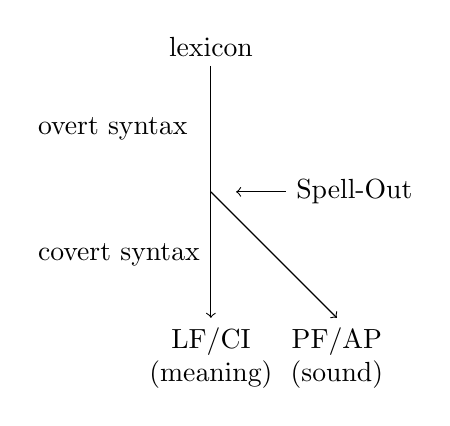
\begin{tikzpicture}[scale=.8]
%\draw (-2.9,-5.8) to[grid with coordinates] (2.7,-0.6);
\draw[->] (0,-1) node[anchor=south] {lexicon} --(0,-5) node[anchor=north, align=center] {LF/CI\\(meaning)};
\draw[->] (0,-3)--(2,-5) node[anchor=north,align=center] {PF/AP\\(sound)};
\draw[<-] (.4,-3)--(1.2,-3) node[anchor=west] {Spell-Out};
%\draw (0,-0.5) node {lexicon};
\draw (-2.9,-2) node[anchor=west] {overt syntax};
\draw (-2.9,-4) node[anchor=west] {covert syntax};
%\draw (0,-6.5) node[align=center] {LF/CI\\(meaning)};
%\draw (2,-5.5) node[align=center] {PF/AP\\(sound)};
\end{tikzpicture}
\end{itemize}

}

\frame{
\frametitle{Phases}

\begin{itemize}
\item Phases: \citet{Chomsky2008a}.
\item Phase is spelled out once it is combined with a head.

\ea
He believes that Peter comes.
\z
\end{itemize}

}


\subsubsection{Valenz, Merkmalsüberprüfung und Agree}
\label{sec-features-minimalism}



\frame{
\frametitle{DP vs.\ NP}


\begin{itemize}
\item Standardannahme im Minimalismus:\\
      \emph{this man} ist eine DP (weil D der Kopf ist, nicht N)

\ea
letters to this man
\z

\pause
\item \emph{him} hat Distribution wie DP, also dieselbe Kategorie:

\ea
letters to him
\z

\end{itemize}
}

\frame{
\frametitle{Valenzrepräsentation über uninterpretierbare Merkmale}


\begin{forest}
baseline
[N 
  [\emph{letters} {[N, pl, \st{\textit{u}P}]}]
  [P
    [\emph{to} {[P, \st{\textit{u}D}]}]
    [\emph{him} {[D]}]]]
\end{forest}

\begin{itemize}
\item \textit{u}D bedeutet, dass ein D gefunden werden muss.
\pause
\item \st{\textit{u}D} bedeutet, dass ein D gefunden wurde.
\end{itemize}

}

\frame{
\frametitle{Valenzrepräsentation und Crash}

\begin{forest}
baseline
[N 
  [\emph{letters} {[N, pl, \st{\textit{u}P}]}]
  [\emph{to} {[P, \textit{u}D]}]]
\end{forest}

\begin{itemize}
\item Objekt ist nicht wohlgeformt, weil \textit{u}D übrig ist.
\item Derivation "`crasht"' an den Interfaces
\end{itemize}

}



\frame[shrink=10]{
\frametitle{Merkmalsüberprüfung mittels Agree}

\eal
\ex[*]{
letters to he
}
\ex[]{
letters to him
}
\zl

\centerline{
\begin{forest}
baseline
[N 
  [\emph{letters} {[N, pl, \st{\textit{u}P}]}]
  [P
    [\emph{to} {[P, \st{\textit{u}D}, \st{acc}]}]
    [\emph{him} {[D, \st{acc}]}]]]
\end{forest}
}

\begin{itemize}
\item Selektionsmerkmale sind atomar, \dash man kann nicht DP[\type{acc}] verlangen.
\item weiterer Mechanismus, der andere Merkmale überprüfen kann: \emph{Agree}
\item über Agree geprüfte Merkmale müssen nicht unbedingt am obersten Knoten präsent sein.
\end{itemize}

}



\subsubsection{Phrasenstruktur und \xbart}

\frame{
\frametitle{Phrasenstruktur und \xbart}

\centerline{
\begin{forest}
%where n children=0{}{},
%sm edges
%for tree={parent anchor=south, child anchor=north,align=center,base=bottom}
[XP
  [specifier]
  [\xbar
    [specifier]
    [\xbar
      [complement] [X] ] ] ]
\end{forest}
}

\begin{itemize}
\item Ob etwas \xbar oder XP ist, hängt davon ab, ob es als Argument benutzt wird oder nicht.
\item vermeidet unschöne unären Verzweigungen der \xbart
\item Probleme: \citew[Abschnitt~2.1]{Brosziewski2003a-u}. 
\end{itemize}

}


\subsubsection{Little \textit{v}}
\label{sec-little-v}

\frame{

\frametitle{Little \textit{v}}

\eal
\ex[*]{
Emily showed himself Benjamin in the mirror.
}
\ex[]{
Peter showed himself Benjamin in the mirror.
}
\zl

\begin{itemize}
\item \emph{himself} kann sich auf Emily, aber nicht auf Benjamin beziehen.

\item \emph{himself} muss höher im Baum sein.
\end{itemize}

}

\frame{
\frametitle{c-command-Anforderungen und ditransitive Verben}

\ea
A node A c-commands B if, and only if A's sister either:\\
\begin{tabular}[t]{@{}l@{~}l@{}}
a. & is B, or\\
b. & contains B
\end{tabular}
\z

\oneline{
\begin{forest}
baseline
[\vbar
 [\textit{show}]
 [\textit{himself}]
 [\textit{Benjamin}]]
\end{forest}
\hfill
\begin{forest}
baseline
[\vbar
   [\vbar
     [\textit{show}]
     [\textit{himself}] ]
 [\textit{Benjamin}]]
\end{forest}
\hfill\hfill
\begin{forest}
baseline
[\littlevbar
 [\textit{show}]
 [VP
   [\textit{himself}]
   [\vbar
    [V]
    [\textit{Benjamin}]]]]
\end{forest}
}
}

\frame{
\frametitle{Ditransitive Verben}

\ea[]{
Peter showed himself Benjamin in the mirror.
}
\z


\begin{itemize}
\item Analyse mit zusätzlichem leeren Verb geht zurück auf \citet{Larson88a}
\item \citet[\page 70]{HK93a-u}: Leeres Verb steuert Kausativsemantik bei.
\item \emph{show} steht in der V-Position und bewegt sich dann zu \textit{v}.
\item \emph{show} bedeutet \emph{see} und bei \littlev kommt dann die kausative Bedeutung dazu,
  woraus sich \relation{cause-see} ergibt \citep[\page 133]{Adger2003a}. 
\end{itemize}

}

\frame{
\frametitle{Ditransitive Verben}
\centerline{
\begin{forest}
baseline
[\vP
  [\textit{Peter}]
  [\littlevbar
   [\textit{v} $+$ \textit{show}]
   [VP
     [\textit{himself}]
     [\vbar
      [\phonliste{ show } {[V]}]
      [\textit{Benjamin}]]]]]
\end{forest}
}
}


\subsubsection{Linking}

\frame{
\frametitle{Little \textit{v} everywhere}

\begin{itemize}
\item Verb-Shell-Analyse ursprünglich nur für ditransitive Verben \citep{Larson88a},\\
 jetzt aber auch für strikt transitive Verben und intransitive Verben verwendet.

\item \citet[Abschnitt~4.5]{Adger2003a}: semantische Rollen einheitlich vergeben:
\eal
\ex DP Tochter von \vP $\to$ interpretiert als agent
\ex DP Tochter von VP $\to$ interpretiert als theme
\ex PP Tochter von \littlevbar $\to$ interpretiert als goal
\zl
\item Adger: einheitlich zugewiesene Rollen helfen bei Spracherwerb,\\
      also \littlev auch bei strikt transitiven und intransitiven Verben.

\item Frage: Involviert \emph{schlafen} eine kausative Komponente? Ein Agens?

\end{itemize}
}

\frame{
\frametitle{Transitive und intransitive Verben}

\vfill
\hfill\begin{forest}
baseline
[\vP
  [Agent]
  [\littlevbar~{[\st{\textit{u}D}]}
   [\textit{v}]
   [VP
      [\textit{burn} {[V, \st{\textit{u}D}]}]
      [Theme]]]]]
\end{forest}
\hfill
\begin{forest}
baseline
[\vP
  [Agent]
  [\littlevbar~{[\st{\textit{u}D}]}
   [\textit{v} ]
   [ \textit{laugh} {[V]} ]]]
\end{forest}
\hfill\mbox{}

\vfill
\begin{itemize}
\item \citet[\page 164]{Adger2003a}:\\
      Auch intransitive und transitive Verben bewegen sich von V nach \textit{v}.
\end{itemize}
\vfill
}

\subsubsection{CP, TP, \vP, VP}
\label{sec-CP-TP-vP-VP}


\subsubsubsection{Merkmale als Auslöser von Bewegungen: Das EPP-Merkmal von T}
\label{sec-epp-features}

\frame{
\frametitle{Merkmale als Auslöser von Bewegung: EPP-Merkmal bei T}

\begin{itemize}
\item In GB waren die Subjekte Spezifikatoren von IP.
\item Jetzt sind sie Spezifikatoren von \vP.
\item Kombiniert man Modalverben mit \vP, steht Subjekt an falscher Stelle.
\eal
\ex[*]{
Will Ann read the book.
}
\ex[]{
Anna will read the book.
}
\zl

\item Annahme eines starken, uninterpretierbaren Merkmals D beim T-Kopf.

\item Starke Merkmale lösen Bewegung aus, weil die Überprüfung lokal erfolgen muss. 
      Sie werden durch ein `*' gekennzeichnet.

\item Da das Merkmal stark ist, muss ein passendes D in die Spezifikatorposition von T bewegt werden
  und das D checken.


\end{itemize}

}

\frame{
\frametitle{Merkmale als Auslöser von Bewegung: EPP-Merkmal bei T}

\centerline{
\scalebox{.8}{%
\begin{forest}
baseline
[TP
 [\textit{Anna} {[D]}]
 [\tbar{[\st{\textit{u}D*}]}
   [\textit{will} T{[pres]}]
   [\vP
     [\phonliste{ Anna }]
     [\littlevbar~{[\st{\textit{u}D}]}
       [\textit{v}
         [\textit{read}] [\textit{v}]]
       [VP
         [\phonliste{ read } {[V, \st{\textit{u}D}]}]
         [DP [\textit{the book}, roof]]]]]]]
\end{forest}
}
}

}

\frame{
\frametitle{EPP: Extended Projection Principle}

\begin{itemize}

\item Das Merkmal wird EPP-Merkmal genannt.\\
      EPP steht für Extended Projection Principle.
\pause

\item EPP gab es schon in der GB: Jeder Satz muss ein Subjekt haben.
\pause

\item Das ist für das Deutsche falsch:
\eal
\ex Mir ist schlecht.
\ex weil noch gearbeitet wurde
\zl

\pause
\item Man kann behaupten, dass in (\mex{0}) leere Subjekte vorliegen,\\das Prinzip wird dadurch aber entwertet.
\end{itemize}
}


\frame{
\frametitle{Komplette Analyse eines Deklarativsatzes mit CP}

\centerline{
\scalebox{.75}{%
\begin{forest}
baseline
[CP
 [C{[Decl]}]
 [TP
 [\textit{Anna} {[D]}]
 [\tbar{[\st{\textit{u}D*}]}
   [\textit{will} T{[pres]}]
   [\vP
     [\phonliste{ Anna }]
     [\littlevbar~{[\st{\textit{u}D}]}
       [\textit{v}
         [\textit{read}] [\textit{v}]]
       [VP
         [\phonliste{ read } {[V, \st{\textit{u}D}]}]
         [DP [\textit{the book}, roof]]]]]]]]
\end{forest}
}
}

}

\frame{
\frametitle{Fragen}

\begin{itemize}
\item Für (\mex{1}) braucht man ein unvalued Satztypen-Merkmal bei T für den Satztyp \emph{question}. 
\ea
What will Anna read?
\z
\item Der leere Komplementierer C hat ein Q-Merkmal, das dem Satztyp-Merkmal bei T einen Wert
  zuweisen kann. (value the feature)
\item Da das Satztypmerkmal bei T strong ist, muss sich das T-Element zu C bewegen, um das Merkmal
  lokal checken zu können.

\item \emph{wh}-Element muss auch bewegt werden. Das wird durch starkes \emph{wh}-Merkmal bei C
  erzwungen.

\end{itemize}

}

\frame{
\frametitle{Fragen: \emph{What will Anna read?}}

\centerline{
\scalebox{.7}{
\begin{forest}
baseline
[CP
 [\textit{what} {[D, wh]}]
 [\cbar{[\st{\textit{u}wh*}]}
   [C
     [\textit{will} T{[\st{Q*}]}]
     [C{[Q]}] ]
   [TP
   [\textit{Anna} {[D]}]
   [\tbar{[\st{\textit{u}D*}]}
     [\phonliste{ will } {[T]}]
     [\vP
       [\phonliste{ Anna }]
       [\littlevbar~{[\st{\textit{u}D}]}
         [\textit{v}
           [\textit{read}] [\textit{v}]]
         [VP
           [\phonliste{ read } {[V, \st{\textit{u}D}]}]
           [\phonliste{what}]]]]]]]]
\end{forest}
}
}
}

\subsubsection{Kasuszuweisung}


\frame{
\frametitle{Kasuszuweisung}

\begin{itemize}
\item Die DPs \emph{Anna} und \emph{the book} haben zu Beginn uninterpretierbare Kasusmerkmale:
[\textit{u}case:]. 
\pause
\item Die Merkmale werden valuiert durch T und \textit{v}.
\pause
\item Nur ein Merkmal wird durch Merge gecheckt. Bei T das D-Merkmal. 
\pause
\item Kasusmerkmal muss mittels eines anderen Checking-Mechanismuses gecheckt werden: Agree.
\pause
\item Agree kann Merkmale in Schwesterknoten checken oder auch weiter weg im Baum.
\pause
\item Knoten muss den Knoten, mit dem es eine Agree-Relation geben soll, c-kommandieren.

\end{itemize}

}

\frame[shrink]{
\frametitle{Kasuszuweisung}

\centerline{
\scalebox{.7}{
\begin{forest}
baseline
[TP
 [\textit{Anna} {[D, \st{nom}]}]
 [\tbar{[\st{\textit{u}D*}, \st{nom}]}
   [T{[pres]}]
   [\vP
     [\phonliste{ Anna }]
     [\littlevbar~{[\st{\textit{u}D}]}
       [\textit{v}
         [\textit{read}] [\textit{v} {[\st{acc}]}]]
       [VP
         [\phonliste{ read } {[V, \st{\textit{u}D}]}]
         [DP{[\st{acc}]} [\textit{the book}, roof]]]]]]]
\end{forest}
}}

\begin{itemize}
\item \textit{v} c-kommandiert VP, V, die DP \emph{the book} und alle Knoten in dieser DP.
\item Da Agree Merkmale von c-kommandierten Knoten valuieren kann,\\
      kann der Akkusativ bei \textit{v} das Kasus-Merkmal der DP \emph{the book} valuen.
\end{itemize}

}


\frame[shrink]{
\frametitle{Nichtlokalität von Agree}

\begin{itemize}
\item Agree kann nicht-lokal Merkmale überprüfen. Aber was ist mit (\mex{1})?
\ea[*]{
\label{ex-him-likes-she}
Him likes she.
}
\z
Der Akkusativ von \textit{v} könnte mit dem Subjekt abgeglichen werden und der Nominativ von T mit
dem Objekt von \emph{likes}.

\centerline{
\scalebox{.7}{
\begin{forest}
baseline
[TP
 [\textit{him} {[D, \st{acc}]}]
 [\tbar{[\st{\textit{u}D*}, \st{nom}]}
   [T{[pres]}]
   [\vP
     [\phonliste{ him }]
     [\littlevbar~{[\st{\textit{u}D},\st{acc}]}
       [\textit{v}
         [\textit{read}] [\textit{v} {[\st{acc}]}]]
       [VP
         [\phonliste{ read } {[V, \st{\textit{u}D}]}]
         [DP{[\st{nom}]} [\textit{she}]]]]]]]
\end{forest}
}}


\end{itemize}
}

\frame{
\frametitle{Nichtlokalität von Agree}

\begin{itemize}
\item Anforderung an Agree: Nimm das nächstmögliche Element.
\item \citet[\page 218]{Adger2003a}:
\ea
\label{principle-locality-of-matching}
Locality of matching\is{locality!of matching}: Agree holds between a feature F on X and a matching feature F on Y if and only
if there is no intervening Z[F].
\z
Intervention ist wie folgt definiert:
\ea
\label{def-intervention}
Intervention\is{intervention}: In a structure [X \ldots{} Z \ldots{} Y], Z intervenes between X and Y iff X
c-commands\is{c"=command} Z and Z c-commands Y.
\z
\item Weil T mit \emph{Anna} Agreen kann, darf es nicht mit \emph{the book} Agreen.
\end{itemize}
}

\subsubsection{Adjunkte}

\frame{
\frametitle{Adjunkte}

\begin{itemize}
\item \citet[Section~4.2.3]{Adger2003a} nimmt an, dass Adjunkte sich mit XP verbinden und eine neue XP
bilden.
\item Er nennt diese Operation \emph{Adjoin}.

\item Operation konsumiert keine Merkmale, ist also anders als External Merge.

\item Das heißt, neue zusätzliche Operation in der Theorie (nicht nur die beiden Merges!).

\item Es gibt Vorschläge, Adjunkte als Elemente innerhalb spezieller adverbieller Phrasen mit leeren
  Köpfen zu behandeln.

\item Ich finde Adgers Lösung besser.\\
      Entspricht dem, was in vielen anderen Frameworks auch gemacht wird.
\end{itemize}

}


\subsection{Verbstellung}
\label{sec-verb-position-MP}

\frame{
\frametitle{Verbstellung}

\begin{itemize}
\item Finites Verb bewegt sich von V zu \textit{v} zu T und dann zu C.
\item Die Bewegung zu T wird durch ein starkes Tense-Merkmal von T erzwungen.
\item Die Bewegung des T-Komplexes nach C wird durch ein Satztypmerkmal ausgelöst, das durch ein
  starkes Interrogativ-Merkmal (Int) bzw. durch ein Deklarativ-Merkmal (Decl) valuiert wird.
\end{itemize}


%% \ea
%% Kennt jeder diesen Roman?
%% \z

}

\frame{
\frametitle{Verbstellung: \emph{Kennt jeder diesen Roman?}}


\scalebox{.7}{
\begin{forest}
[CP
    [C
      [T{[\st{Int*}]}
        [\textit{kennt} {[\st{Pres*}]}]
        [T{[Pres]}]]
      [C{[Int]}]]
    [TP
      [\textit{jeder}]
      [\tbar{[\st{\textit{u}D*}]}
        [\vP
          [\phonliste{ jeder }]
          [\littlevbar
            [VP
              [DP [\textit{diesen Roman}, roof] ]
              [\phonliste{ kennt }]]
            [\textit{v}
              [\phonliste{ kennt }]
              [\textit{v}]]]]
        [\phonliste{ kennt T }]]]]
\end{forest}
}
}


\subsection{Fernabhängigkeiten}

\frame{
\frametitle{Fernabhängigkeiten}

\begin{itemize}
\item Decl bei C löst Verbumstellung aus.
\item Merkmal top löst Bewegung nach SpecCP aus.
\end{itemize}
}

\frame{
\frametitle{Fernabhängigkeiten \emph{Diesen Roman kennt jeder.}}

\scalebox{.7}{
\begin{forest}
[CP
  [\emph{diesen Roman} {[top] }]
  [\cbar{[\st{\textit{u}top*}]}
    [C
      [T{[\st{Decl*}]}
        [\textit{kennt} {[\st{Pres*}]}]
        [T{[Pres]}]]
      [C{[Decl]}]]
    [TP
      [\textit{jeder}]
      [\tbar{[\st{\textit{u}D*}]}
        [\vP
          [\phonliste{ jeder }]
          [\littlevbar
            [VP
              [\phonliste{ diesen Roman }{[D]}]
              [\phonliste{ kennt }]]
            [\textit{v}
              [\phonliste{ kennt }]
              [\textit{v}]]]]
        [\phonliste{ kennt T }]]]]]
\end{forest}
}
}


\subsection{Passiv}

\frame{
\frametitle{Passiv}


\begin{itemize}
\item Wie bei GB weist Verb keinen Akk zu: \littlev hat kein acc-Merkmal.
\item Dafür spezielle Version von \littlev, das auch bei den unakkusativischen Verben eine Rolle spielt \citep{Perlmutter78}.

\citet[\page 140]{Adger2003a}: \vPs für unakkusativische Verben \emph{fall}, \emph{collapse}, \emph{wilt}:

\vfill

\begin{forest}
[\vP
  [\textit{v}]
  [VP
    [\textit{fall}{[V, \textit{u}D]}]
    [Theme]]]
\end{forest}

\vfill

\item Unakkusativisches \littlev spielt auch bei Analyse des Passivs eine Rolle.
\item Es gibt ein Subjekt, das irgendwie Objekteigenschaften hat.
\item Das spezielle \littlev wird von einem Passivkopf \emph{werden} gefordert und\\
      bildet eine Passive Phrase.

\end{itemize}

}

\frame{
\frametitle{Passiv: \emph{dass er geschlagen wurde}}

\centerfit{
%\begin{sideways}  
\begin{forest}
for tree={fit=rectangle}
[TP
     [PassP
       [\vP
         [VP
           [pronoun {[\st{nom}]} ]
           [\phonliste{schlagen}]]
         [\textit{v}
           [\textit{schlagen}]
           [{\textit{v}[\st{\textit{u}Infl}:Pass]}]]]
       [\phonliste{werden}]]
     [{T[past,\st{nom}]}
       [\textit{werden} {[Pass,\st{\textit{u}Infl}:past*]}]
       [{T[past]}]]]
\end{forest}
%\end{sideways}
}

\begin{itemize}
\item Pass-Kopf verlangt Infl-Merkmal von \littlev mit Wert Pass.
\item Partizip-Morphologie bei Spell-Out.
\item Hilfsverb bewegt sich zu T, um starkes Infl zu checken.
\item Weil Infl-Wert past ist, muss Form \emph{wurde} ausgesprochen werden
\item Es gibt keine Bewegung! Kasus wird über Agree vergeben.
\end{itemize}


}

\frame{
\frametitle{Passiv: Aber}

\begin{itemize}
\item Das ist besser als bei der GB-Analyse mit IP.
\item Aber: \citet[\page 332]{Adger2003a} nimmt für Deutsch an, dass es ein starkes EPP-Merkmal
  gibt.
\item Daraus ergeben ich dieselben Probleme wie beim GB-Ansatz.
\item Alle Objekte müssen sich zu T bewegen, auch wenn es keine Umstellung im Satz gibt.
\item Unpersönliche Passive sind problematisch, da es nichts gibt,\\
      was sich zu T bewegen könnte.
\ea
weil getanzt wurde
\z
\end{itemize}
}


\subsection{Lokale Umstellung}

\frame{
\frametitle{Lokale Umstellung}

\begin{itemize}
\item \citet{Adger2003a} behandelt Scrambling nicht.
\item Alle Umordnungen sind merkmalsgesteuert, also muss es irgendein Merkmal geben, das
  Umstellungen wie in (\mex{1}b) auslöst:
\eal
\ex 
{}[weil] jeder diesen Roman kennt
\ex 
{}[weil] diesen Roman jeder kennt
\zl
\item Diverse Vorschläge in der Literatur mit so genannten funktionalen Projektionen:
\begin{itemize}
\item Topic Phrase \citep[\page 222]{Laenzlinger2004a} 
\item AgrS und AgrO \citep[Kapitel~4]{Meinunger2000a}
\end{itemize}
\item Bessere Lösung von G.\ \citet[Abschnitt~3.5]{GMueller2014a-u}:
      Objekt bewegt sich zu zweiter Spezifikatorposition von \littlev. 
\item Dazu werden optionale Merkmale bei \textit{v} und V angenommen (S.\,48).
\end{itemize}
} 

\frame{
\frametitle{Lokale Umstellung \emph{dass diesen Roman jeder kennt}}

\scalebox{.8}{
\begin{forest}
[CP
    [C
      [dass]]
    [TP
        [\vP
          [\emph{diesen Roman}]
          [\littlevbar
            [ \emph{jeder}]
            [\littlevbar
                [VP
                  [\phonliste{ diesen Roman } {[D]}] 
                  [\phonliste{ kennt }]]
                [\textit{v}
                  [\phonliste{ kennt }]
                  [\textit{v}]]]] ]
        [\textit{kennt} {[T]}]]]
\end{forest}
}

}

\frame{
\frametitle{Überblick über Stipulationen}

\begin{itemize}
\item Annahmen in Adgers Analyse:
\begin{itemize}
\item Kategorie eines Knotens hängt davon ab, wie er verwendet wird (noch erweitert oder nicht).
\item Bei Merge kann immer genau ein Merkmal überprüft werden.
\item Andere Merkmale werden mit Agree überprüft.
\item Agree kann Merkmale überprüfen, wenn c-Kommando vorliegt.
\item Agree kann nur dann Merkmale überprüfen, wenn kein anderes Merkmal interveniert.
\item Es gibt starke und schwache Merkmale.
\item Derivationen, die noch Merkmale übrig haben, crashen an den Interfaces.
\end{itemize}
\pause
\item Es gibt ein Spracherwerbsproblem.
\pause
\item Zum Vergleich CG und HPSG:
\begin{itemize}
\item Es gibt einen Funktor mit einer Beschreibung des abhängigen Elements.
\item Abhängiges Element muss passen.
\end{itemize}
\pause
\item Adgers Analyse ist die MP-Analyse mit den wenigsten Stipulationen.
\end{itemize}


}

\subsection{Varianten und Argumentation für Theorien}

\frame{
\frametitle{Varianten und Argumentation für Theorien}

\begin{itemize}
\item Es gibt viele Varianten und Sub-Schulen.
\item Kartographie (Crypto-Konstruktivismus): Probleme mit der Syntax-Semantik-Trennung werden durch
  Syntaktifizierung der Semantik umgangen \citep{Rizzi2014a}
\item Kaynesche Ansätze mit zugrundeliegender Specifier-Head-Complement-Anordnung für alle Sprachen.
\item \ldots
\end{itemize}


}

\frame{
\frametitle{Varianten: \citet{Rizzi97a-u}}

\scalebox{.5}{%
\newlength\mytextheight
\settototalheight{\mytextheight}{XpX$^0$X$'$}
\begin{forest}
  delay={
    where content={}{
      content={\phantom{X}}
    }{},
  },
  for tree={
    text height=\mytextheight,
    fit=band,
    parent anchor=south,
    child anchor=north,
  }
[ForceP
	[]
	[Force$'$
		[Force$^0$]
		[TopP*
			[]
			[Top$'$
				[Top$^0$]
				[FocP
					[]
					[Foc$'$
						[Foc$^0$]
						[TopP*
							[]
							[Top$'$
								[Top$^0$]
								[FinP
									[]
									[Fin$'$
										[Fin$^0$]
										[IP]]]]]]]]]]]
\end{forest}
}

}


\frame{
\frametitle{Evidence from a single language and UG}


\begin{itemize}
\item What does it mean for other languages\\
      that a rule/morpheme is present in one particular language?
\pause
\item Possible answer:\\
      If we have a certain structure in language X,\\
      it must be present in all languages.
\pause
\item Example:
      \begin{itemize}
      \item Basque: Tree positions for object agreement (AgrO, AgrIO)\nocite{Chomsky93b-u,Stechow96a,Grewendorf2002a,Meinunger2000a}
      \item Japanese/Gungbe: Tree position for topic marker\nocite{CR2010a} %\citet[\page 62]{CR2010a}
      \end{itemize}

\pause
\item German and Dutch neither have object agreement nor topic morphemes.

\pause
\item Conclusion:\\
      If such inferences regarding properties of particular languages are made,\\
      one has to assume (very specific!) innate linguistic knowledge.

\end{itemize}

% Parameter
\nocite{Newmeyer2005a}
}

%% \frame[shrink]{
%% \frametitle{AgrS, AgrIO und AgrO nach \citew[S.\,101]{Meinunger2000a}}

%% \begin{columns}[T]

%% \begin{column}{65mm}
%% \scalebox{0.4}{\begin{pspicture}(1.6,0)(17.4,16.3)
%% %\psgrid
%% %% \only<handout>{\psline[linewidth=5mm,linecolor=red](3,14)(16,1)
%% %% \psline[linewidth=5mm,linecolor=red](3,1)(16,14)}
%% \rput[B](3,0){\rnode{die Firma}{die Firma Müller}}
%% \rput[B](6,0){\rnode{meinem Onkel}{meinem Onkel}}
%% \rput[B](9,0){\rnode{diese Moebel}{diese Möbel}}
%% \rput[B](12,0){\rnode{erst gestern}{erst gestern}}
%% \rput[B](15,0){\rnode{zugestellt}{zugestellt}}
%% \rput[B](17,0){\rnode{hat}{hat}}
%% %
%% \rput[B](14,2){\rnode{tdo}{t\sub{DO}}}
%% \rput[B](15,2){\rnode{v}{V}}
%% \rput[B](14.5,3){\rnode{vp1}{VP}}
%% %
%% \rput[B](13.5,3){\rnode{tio}{t\sub{IO}}}
%% \rput[B](14,4){\rnode{vs}{V'}}
%% %
%% \rput[B](13,4){\rnode{tsu}{t\sub{SU}}}
%% \rput[B](13.5,5){\rnode{vp2}{VP}}
%% %
%% \rput[B](12,5){\rnode{adv}{Adv}}
%% \rput[B](13,6){\rnode{vp3}{VP}}
%% %
%% \rput[B](15,6){\rnode{agro0}{AgrO$^0$}}
%% \rput[B](14,7){\rnode{agros}{AgrO'}}
%% %
%% \rput[B](9,7){\rnode{do}{DO}}
%% \rput[B](11.5,9){\rnode{agrop}{AgrOP}}
%% %
%% \rput[B](13.5,9){\rnode{agrio0}{AgrIO$^0$}}
%% \rput[B](12.5,10){\rnode{agrios}{AgrIO'}}
%% %
%% \rput[B](6,10){\rnode{io}{IO}}
%% \rput[B](9.25,12){\rnode{agriop}{AgrIOP}}
%% %
%% \rput[B](17,12){\rnode{agrs0}{AgrS$^0$}}
%% \rput[B](13.125,14){\rnode{agrss}{AgrS'}}
%% %
%% \rput[B](3,14){\rnode{su}{SU}}
%% \rput[B](8.06125,16){\rnode{agrsp}{AgrSP}}
%% %
%% \psset{angleA=-90,angleB=90,arm=0pt}
%% %
%% \ncdiag{vp1}{v}
%% \ncdiag{vp1}{tdo}
%% %
%% \ncdiag{vs}{tio}
%% \ncdiag{vs}{vp1}
%% %
%% \ncdiag{vp2}{vs}
%% \ncdiag{vp2}{tsu}
%% %
%% \ncdiag{vp3}{vp2}
%% \ncdiag{vp3}{adv}
%% %
%% \ncdiag{agros}{vp3}
%% \ncdiag{agros}{agro0}
%% %
%% \ncdiag{agrop}{agros}
%% \ncdiag{agrop}{do}
%% %
%% \ncdiag{agrios}{agrop}
%% \ncdiag{agrios}{agrio0}
%% %
%% \ncdiag{agriop}{agrios}
%% \ncdiag{agriop}{io}
%% %
%% \ncdiag{agrss}{agriop}
%% \ncdiag{agrss}{agrs0}
%% %
%% \ncdiag{agrsp}{agrss}
%% \ncdiag{agrsp}{su}
%% %
%% \pstriangle(3,0.4)(2.6,13.5)
%% \pstriangle(6,0.4)(2.3,9.5)
%% \pstriangle(9,0.4)(1.9,6.5)
%% \pstriangle(12,0.4)(1.7,4.5)
%% \ncdiag{v}{zugestellt}
%% \ncdiag{agrs0}{hat}
%% %% \only<beamer>{\only<3->{\psline[linewidth=5mm,linecolor=red](3,14)(16,1)
%% %% \psline[linewidth=5mm,linecolor=red](3,1)(16,14)}}
%% \end{pspicture}}
%% \end{column}
%% \begin{column}{55mm}
%% {\footnotesize
%% \begin{itemize}
%% \item Objektkongruenz im Baskischen.

%%       Wir modellieren das mit Baumkonfigurationen. $\to$

%%       Es muss die Konfigurationen in allen Sprachen geben.
%% \pause
%% \item Wenn wir den Baum schon mal haben, können
%%       wir ihn für die Modellierung d.\ Informationsstruktur im Deutschen benutzen.
%% \pause
%% \item Nein! Kongruenz ist eine Eigenschaft der beteiligten Objekte:\\
%%       die Gleichheit von Werten.

%%       Konfigurationale Aspekte sind dabei irrelevant.
%% \end{itemize}
%% }
%% \end{column}
%% \end{columns}

%% }



\frame{
\frametitlefit{Deutsch ist Englisch/Romanisch (SVO, Laenzlinger nach Kayne)}

\nocite{Laenzlinger2004a,Kayne94a-u}
\begin{columns}[T]

\begin{column}{80mm}
\mode<beamer>{%
\scalebox{0.5}{
\small
\psset{xunit=10mm,yunit=6mm}
%
\begin{pspicture}(-0.4,3)(16.2,20.8)
\rput[B](2,20){\rnode{CP}{CP}}
\rput[B](0,18){\rnode{C}{\cnull}}
\rput[B](4,18){\rnode{SubjP}{SubjP}}
\rput[B](2,16){\rnode{SpecSubjP}{\alt<32->{DP}{XP}}}
\rput[B](6,16){\rnode{ObjP}{\ldots ObjP}}
\rput[B](4,14){\rnode{SpecObjP}{\alt<15->{DP}{XP}}}
\rput[B](8,14){\rnode{AuxP}{\ldots AuxP}}
\rput[B](6,12){\rnode{SpecAuxP}{\alt<49->{VP}{XP}}}
\rput[B](10,12){\rnode{AuxPlus}{Aux+}}
\rput[B](8,10){\rnode{Aux}{Aux}}
\rput[B](12,10){\rnode{vP}{$\nu$P}}
\rput[B](10,8){\rnode{SpecvP}{DP}}
\rput[B](14,8){\rnode{VP}{VP}}
\rput[B](12,6){\rnode{V}{\visible<beamer| beamer:-36>{V}}}
\rput[B](16,6){\rnode{ObjDP}{\visible<beamer| beamer:-36>{DP}}}
%
\psset{angleA=-90,angleB=90,arm=0pt}
%
\ncdiag{CP}{C}\ncdiag{CP}{SubjP}
\ncdiag{SubjP}{SpecSubjP}\ncdiag{SubjP}{ObjP}
\ncdiag{ObjP}{SpecObjP}\ncdiag{ObjP}{AuxP}
\ncdiag{AuxP}{SpecAuxP}\ncdiag{AuxP}{AuxPlus}
\ncdiag{AuxPlus}{Aux}\ncdiag{AuxPlus}{vP}
\ncdiag{vP}{SpecvP}\ncdiag{vP}{VP}
%
\rput[B](0,4){\rnode{weil}{weil}}
\rput[B](2,4){\rnode{er-vorn}{\visible<beamer| beamer:-32>{[ \_ ]}}}
\rput[B](4,4){\rnode{ihn-vorn}{\visible<beamer| beamer:-15>{[ \_ ]}}}
\rput[B](6,4){\rnode{gelesen-vorn}{\visible<beamer| beamer:-49>{[ \_ ]}}}
\rput[B](8,4){\rnode{hat}{hat}}
\rput[B](10,4){\rnode{er}{\visible<beamer| beamer:-18>{er}}}
\rput[B](12,4){\rnode{gelesen}{\visible<beamer| beamer:-35>{gelesen}}}
\rput[B](14,4){\rnode{trace-VP}{\visible<beamer| beamer:37->{[ \_ ]$_k$}}}
\rput[B](16,4){\rnode{ihn}{\visible<beamer| beamer:1>{ihn$_j$}}}
%
\ncdiag{C}{weil}
\ncdiag{SpecSubjP}{er-vorn}
\ncdiag{SpecObjP}{ihn-vorn}
\visible<beamer| beamer:-49>{\ncdiag{SpecAuxP}{gelesen-vorn}}
\ncdiag{Aux}{hat}
\ncdiag{SpecvP}{er}

\alt<-36>{
\ncdiag{VP}{V}\ncdiag{VP}{ObjDP}
\ncdiag{V}{gelesen}
\ncdiag{ObjDP}{ihn}
}{
\ncdiag{VP}{trace-VP}
}

\visible<beamer| beamer:50->{\pstriangle(6,4.6)(2,7.2)}
%\pscircle(12,8.5){1.9}
%\psline{->}(12,5.4)(12,5)(6,5)(6,5.6)
%\psline{->}(14,7.8)(14,4)(4,4)(4,5.6)
% 16 * .75 = 12
%  4 * .6  = 2.4
%
% 10 * .75 = 7.5 
%  2 * .75 = 1.5
\tmove<2-17>(16cm,2.4cm)(4cm,2.4cm){ihn$_j$}{\visible<beamer| beamer:-36>{[ \_ ]$_j$}}
\tmove<19-34>(10cm,2.4cm)(2cm,2.4cm){er$_i$}{[ \_ ]$_i$}
% The whole VP is the trace.
\tmove<36-51>(12cm,2.4cm)(6cm,2.4cm){[gelesen [ \_ ]$_j$ ]$_k$}{}
%\psgrid
%
\end{pspicture}
}
}
\mode<handout>{%
\scalebox{0.5}{
\small
\psset{xunit=9mm,yunit=6mm}
%
\begin{pspicture}(-0.4,1)(16.2,20.8)
\rput[B](2,20){\rnode{CP}{CP}}
\rput[B](0,18){\rnode{C}{\cnull}}
\rput[B](4,18){\rnode{SubjP}{SubjP}}
\rput[B](2,16){\rnode{SpecSubjP}{DP}}
\rput[B](6,16){\rnode{ObjP}{\ldots ObjP}}
\rput[B](4,14){\rnode{SpecObjP}{DP}}
\rput[B](8,14){\rnode{AuxP}{\ldots AuxP}}
\rput[B](6,12){\rnode{SpecAuxP}{VP}}
\rput[B](10,12){\rnode{AuxPlus}{Aux+}}
\rput[B](8,10){\rnode{Aux}{Aux}}
\rput[B](12,10){\rnode{vP}{$\nu$P}}
\rput[B](10,8){\rnode{SpecvP}{DP}}
\rput[B](14,8){\rnode{VP}{VP}}
\rput[B](12,6){\rnode{V}{{V}}}
\rput[B](16,6){\rnode{ObjDP}{{DP}}}
%
\psset{angleA=-90,angleB=90,arm=0pt}
%
\ncdiag{CP}{C}\ncdiag{CP}{SubjP}
\ncdiag{SubjP}{SpecSubjP}\ncdiag{SubjP}{ObjP}
\ncdiag{ObjP}{SpecObjP}\ncdiag{ObjP}{AuxP}
\ncdiag{AuxP}{SpecAuxP}\ncdiag{AuxP}{AuxPlus}
\ncdiag{AuxPlus}{Aux}\ncdiag{AuxPlus}{vP}
\ncdiag{vP}{SpecvP}\ncdiag{vP}{VP}
%
\rput[B](0,4){\rnode{weil}{weil}}
\rput[B](2,4){\rnode{er-vorn}{er}}
\rput[B](4,4){\rnode{ihn-vorn}{ihn}}
\rput[B](6,4){\rnode{gelesen-vorn}{gelesen}}
\rput[B](8,4){\rnode{hat}{hat}}
%\rput[B](10,4){\rnode{er}{\visible<beamer| beamer:-18>{er}}}
%\rput[B](12,4){\rnode{gelesen}{\visible<beamer| beamer:-35>{gelesen}}}
%\rput[B](14,4){\rnode{trace-VP}{\visible<beamer| beamer:37->{[ \_ ]$_k$}}}
%\rput[B](16,4){\rnode{ihn}{\visible<beamer| beamer:1>{ihn$_j$}}}
%
\ncdiag{C}{weil}
\ncdiag{SpecSubjP}{er-vorn}
\ncdiag{SpecObjP}{ihn-vorn}
\ncdiag{SpecAuxP}{gelesen-vorn}
\ncdiag{Aux}{hat}
\ncdiag{SpecvP}{er}

\ncdiag{VP}{V}\ncdiag{VP}{ObjDP}
\ncdiag{V}{gelesen}
\ncdiag{ObjDP}{ihn}

\visible<beamer| beamer:50->{\pstriangle(6,4.6)(2,7.2)}
\pscircle(14,6.5){2.3}
\psline{->}(10,7.8)(10,3)(2,3)(2,3.6)
\psline{->}(14,2.6)(14,2)(6,2)(6,3.6)
\psline{->}(16,5.8)(16,1)(4,1)(4,3.6)
%\psgrid
%
\end{pspicture}
}
}
\end{column}
\begin{column}{40mm}
\footnotesize
\begin{itemize}
\item All languages are Spr-H-Comp underlyingly.
\item<2-> The object is moved out of the VP.
\item<19-> The subject is fronted.
\item<36-> The empty VP is fronted.
\item<52-> There are further empty heads \citep{Cinque99a-u}.
\item<53-> Innateness has to be assumed.
\end{itemize}
\end{column}
\end{columns}

\pause
\pause
\pause
\pause
\only<54>{}


\nocite{Haider2000a}
% against remnant movement
\nocite{Fanselow2002a}


}


\frame{
\frametitle{Deutsch ist Deutsch (GB-Varianten, CG, LFG, HPSG, \ldots)}


\centerline{%
\begin{forest}
sm edges
[CP
 [C [weil]]
 [VP
   [NP [er]]
   [V$'$
     [NP [ihn]]
     [V
       [V [gelesen]]
       [V [hat]]]]]]
\end{forest}
\hfill
\begin{forest}
sm edges
[CP
 [C [weil]]
 [VP
   [NP [er]]
   [NP [ihn]]
   [V [gelesen]]
   [V [hat]]]]
\end{forest}
}

\nocite{Fanselow2001a,CJ2005a,BvN98a}

}

%\fi

\frame{
\frametitle{English, German, \ldots{} are Hungarian}
\begin{columns}[T]

\begin{column}{35mm}
\scalebox{0.65}{
\psset{xunit=5mm,yunit=5mm}
\begin{pspicture}(-1.6,0)(8.6,11)
\rput[B](1.5,10){\rnode{AgrP}{\alert<beamer| beamer:1>{AgrP}}}
\rput[B](-1,8){\rnode{SpecAgrP}{\alt<34->{DP}{XP}}}
\rput[B](-1,0){\rnode{mir}{\visible<beamer| beamer:35->{mir$_j$}}}
\rput[B](4,8){\rnode{Agrs}{\alert<beamer| beamer:1>{Agr$'$}}}
\rput[B](2,6){\rnode{Agr}{\alert<beamer| beamer:1>{Agr}}}
\rput[B](2,0){\rnode{Agrw}{\visible<beamer| beamer:-14>{\trace}}}
\rput[B](6,6){\rnode{PP}{PP}}
\rput[B](6,4){\rnode{Ps}{P$'$}}
\rput[B](4,2){\rnode{P}{P}}
\rput[B](4,0){\rnode{in}{\visible<beamer| beamer:-1>{hinter}}}
\rput[B](8,2){\rnode{DP}{DP}}
\rput[B](8,0){\rnode{dS}{\visible<beamer| beamer:-19>{mir}}}
%
\psset{angleA=-90,angleB=90,arm=0pt}
%
\alert<1>{\ncdiag{AgrP}{SpecAgrP}\ncdiag{AgrP}{Agrs}%
\ncdiag{Agrs}{Agr}\ncdiag{Agrs}{PP}%
\ncdiag{Agr}{Agrw}}%
\ncdiag{PP}{Ps}%
\ncdiag{Ps}{P}\ncdiag{Ps}{DP}%
\ncdiag{P}{in}
\ncdiag{DP}{dS}
\visible<33->{\ncdiag{SpecAgrP}{mir}}
%\psgrid
\tmove<2-17>(2cm,0cm)(1cm,0cm){hinter$_i$}{\trace$_i$}
\tmove<19-34>(4cm,0cm)(-0.5cm,0cm){mir$_j$}{\trace$_j$}
\end{pspicture}

}
\end{column}
\begin{column}{85mm}
\begin{itemize}
\item<1-> \citet*[p.\,124]{HNG2005a}: agreement head for the checking of case features
\item<2-> Preposition is moved there.
\item<19-> DP is put into the specifier position of this head.
\item<36-> Evidence for this:\\ Agreement in Hungarian postpositional phrases
\item<37-> English is like Hungarian,\\
      but the movement is invisible.
\end{itemize}
\end{column}
\end{columns}
}


%\if 0
\frame{
\frametitle{Deutsch ist Deutsch, \ldots{} Ungarisch ist Ungarisch}

\begin{columns}[T]

\begin{column}{35mm}
\scalebox{0.7}{
\psset{xunit=5mm,yunit=5mm}
\begin{pspicture}(-1,0)(4.6,5)
\rput[B](2,4){\rnode{PP}{PP}}
\rput[B](0,2){\rnode{P}{P}}
\rput[B](4,2){\rnode{DP}{DP}}
\rput[B](0,0){\rnode{hinter}{hinter}}
\rput[B](4,0){\rnode{mir}{mir}}
%
\psset{angleA=-90,angleB=90,arm=0pt}
%
\ncdiag{PP}{P}\ncdiag{PP}{DP}
\ncdiag{P}{hinter}\ncdiag{DP}{mir}
%\psgrid
\end{pspicture}
}
\end{column}
\begin{column}{85mm}
\begin{itemize}[<+->]
\item A PP is a P together with an NP (or DP).
\item No movement instead of two movements.
\item Structure has five nodes less.
\item Truly minimal!
\item Question: What constitutes an explanation?\\
      Where and how is complexity of language represented?
\end{itemize}
\end{column}
\end{columns}


}


\frame{
\frametitle{Der Schweizer Käse}

\begin{columns}[T]
\begin{column}{55mm}
\scalebox{.8}{%
\begin{forest}
sm edges without translation
[pP
   [p
	[P [with]]
	[p [$\varnothing$]]]
   [AgrOP
	[D [\textbf{me}]]
	[$\overline{\mbox{AgrO}}$
		[AgrO
			[P [t$'$]]
			[AgrO [,phantom  ]]]
		[PP
			[P [t]]
			[D [\textbf{t}]]]]]]
\end{forest}}
\end{column}
\begin{column}{65mm}
\begin{itemize}
\item from another text book:\\
      \citet[\page 452]{Radford97a-u}
\item \citet[\page 549--550]{Sternefeld2006a-u} calls this a Swiss Cheese analysis, but there are more holes (5) than cheese (2).
\end{itemize}
\end{column}
\end{columns}
}


\subsection{Fundamentale Probleme}

\frame{
\frametitle{Fundamentale Probleme: Kopflose Strukturen}


\begin{itemize}
\item Annahme: Es gibt immer einen Kopf und Strukturen sind binär.
\item Problematisch sind NPN-Konstruktionen \citep{Jackendoff2008a,Bargmann2015a,MuellerCxG}:

\eal
\ex Student after student left the room.
\ex
\label{ex-npn-iteration}
Day after day after day went by, but I never found the courage to talk to
her. \citep{Bargmann2015a}
\zl

\item Jackendoff: 
\begin{itemize}
\item Weder N noch P kann sinnvoll als Kopf bezeichnet werden. 
\item \xbart nicht anwendbar.
\item Semantik nicht kompositional.
\end{itemize}

\end{itemize}



}


\frame{
\frametitle{Fundamentale Probleme: Kopflose Strukturen}


\begin{itemize}

\item G.\,\citet{GMueller2011a} schlägt vor, NPN als Reduplikation zu analysieren: Besondere Form der
  Präposition löst Verdopplung aus.

\item Behauptung: Im Deutschen gäbe es keine NPN-Konstruktionen mit Adjektiven. Ist falsch:
\ea
Die beiden tauchten nämlich geradewegs wieder aus dem heimischen Legoland auf, wo sie im
Wohnzimmer, schwarzen Stein um schwarzen Stein, vermeintliche Schusswaffen nachgebaut
hatten.\footnote{
  taz, 05.09.2018, S.\,20
}
\z
\item Außerdem funktioniert Reduplikation nicht für Iteration wie in (\mex{1}).
\ea
Day after day after day went by, but I never found the courage to talk to
her. \citep{Bargmann2015a}
\z


\end{itemize}



}

%      <!-- Local IspellDict: en_US-w_accents -->

% %\include{formgram-psycho}
% %% -*- coding:utf-8 -*-


\section{Zusammenfassung}


\frame{
\frametitle{Kopflose, idiosynkratische Strukturen}

\begin{itemize}
\item Es gibt Strukturen, die nicht der \xbart entsprechen.

\citet{Matsuyama2004a} und \citet{Jackendoff2008a}:
\eal
\ex Student after student left the room.
\ex
\label{ex-npn-iteration}
Day after day after day went by, but I never found the courage to talk to
her. \citep{Bargmann2015a}
\zl

\pause

\item Diese sind problematisch für CG, DG und Minimalismus, weil diese Theorien einen Kopf/Funktor
  verlangen.

\pause
\item GPSG, LFG, HPSG, CxG, TAG haben damit kein Problem, weil man beliebige Strukturen mit einer
  Bedeutung kombinieren kann.

\end{itemize}


}

\frame{
\frametitle{Übersicht}


\oneline{%
\begin{tabular}{@{}lllll@{}}
Theorie & V1                & V2                     & Passiv       & Scrambling\\
GB      & Bewegung          & Bewegung               & lexikalisch  & Bewegung/Basisgenerierung\\
GPSG    & ID/LP flach       & \slasch                & Metaregel    & ID/LP flach\\
LFG     & co-heads          & functional uncertainty & Lexikonregel & Unterspezifikation von Kasus\\
CG      & direkt/leerer Kopf & Typanhebung \ldots    & Lexikonregel & direkte Kombination\\
HPSG    & \dsl (Kopfbewegung) & \slasch (X(P)-Bewegung) & Lexikonregel  & direkte Kombination\\     
SBCG    & ist HPSG-Variante\\
CxG     & flach?            & flach?                 & Allostruktion & ? Unterspezifikation ID/LP?\\
Minimalism & Bewegung       & Bewegung               & alternatives \textit{v} & Bewegung/Basisgenerierung\\
\end{tabular}}


}

\frame{
\frametitle{Zusammenfassung der gesamten Veranstaltung}

\begin{itemize}
\item Irgendwie machen wir alle dasselbe.
\item Irgendwie dann aber doch nicht.
\end{itemize}



}



\appendix
% muß immer geladen werden, wegen Referenzen
%\section<presentation>*{Literatur}

%% \frame{
%%   \frametitle<presentation>{Literatur}
  
%%   \beamertemplatebookbibitems

%% \bibliography{biblio}
%% \bibliographystyle{natbib.myfullname}
%% }
%\beamertemplatebookbibitems

% there seems to be a bug. These things are only set on the first literature slide
%
% The bug is still there, but the fix does not work any longer. 
\def\insertsectionhead{\refname}
\def\insertsubsectionhead{}

\huberlinjustbarfootline

\ifpdf
\else
\ifxetex
\else
\let\url=\burl
\fi
\fi
\begin{multicols}{2}
{\renewcommand*{\bibfont}{\tiny}

%\beamertemplatearticlebibitems

%\bibliography{bib-abbr,biblio,crossrefs}
%\bibliographystyle{unified}

% biblatex

%\addbibresource{bib-abbr.bib,biblio.bib}

% no book icon please
\setbeamertemplate{bibliography item}{}

%\printbibliography
\printbibliography[heading=bibliography,notkeyword=this] 

}
\end{multicols}




\end{document}


% Local variables:
% mode: lazy-lock
% End:
